\documentclass{book}

\title{
  Zelig: Everyone's Statistical Software\thanks{The current version of
  this software is available at 
  \url{http://gking.harvard.edu/zelig}, free of charge and open-source
  (under the terms of the GNU GPL, v2)}
}
\author{
  Matt Owen\thanks{Statistical Programmer, Institute for Quantitative Social
  Sciences, Harvard University; \url{http://people.iq.harvard.edu/\~mowen/},
  \texttt{mowen@iq.harvard.edu}}
  \and
  Kosuke Imai\thanks{Assistant Professor, Department of Politics,
  Princeton University
  (Corwin Hall, Department of Politics, Princeton University, Princeton NJ 08544;
  \url{http://imai.princeton.edu/}, \texttt{kimai@princeton.edu})}
  \and
  Gary King\thanks{Albert J. Weatherhead III University Professor, Harvard
  University (Institute for Quantitative Social Sciences, 1737 Cambridge 
  Street, Harvard University, Cambridge MA 02138;
  \texttt{http://gking.harvard.edu}, \texttt{king@harvard.edu},
  (617) 495-2027).}
  \and
  Olivia Lau\thanks{Ph.D. Candidate, Department of Government, Harvard
  University (1737 Cambridge Street, Cambridge MA 02138;
  \texttt{http://www.people.fas.harvard.edu/\~\,olau},
  \texttt{olau@fas.harvard.edu}).}
}
\date{\today
}
% packages
\usepackage{Code}
\usepackage{bibentry}
\usepackage{graphicx}
\usepackage{natbib}
\usepackage{amsmath}
\usepackage{url}
\usepackage{Zelig}
\usepackage{Sweave}
\usepackage{upquote}
\usepackage{amssymb}
\usepackage{amsfonts}
\usepackage{verbatim}
\usepackage{epsf}
\usepackage{html}
\usepackage{dcolumn}
\usepackage{multirow}
\usepackage{fullpage}
\usepackage{lscape}

\begin{document}
\maketitle
\tableofcontents

% Part: INTRO
\part{Introduction}
\label{part:Introduction}

\chapter[Introduction]{Introduction to Zelig}
\label{chapter:Intro}
\chapter{Introduction}

\section{What Zelig and R Do}

Zelig\footnote{Zelig is named after a Woody Allen movie about a man
  who had the strange ability to become the physical reflection of
  anyone he met --- Scottish, African-American, Indian, Chinese, thin,
  obese, medical doctor, Hassidic rabbi, anything --- and thus to fit
  well in any situation.} is an easy-to-use program that can estimate
and help interpret the results of an enormous and growing range of
statistical models.  It literally \emph{is} ``everyone's statistical
software'' because Zelig's unified framework incorporates everyone
else's (R) code.  We also hope it will \emph{become} ``everyone's
statistical software'' for applications, and we have designed Zelig so
that anyone can use it or add their models to it.

When you are using Zelig, you are also using
\hlink{R}{http://www.r-project.com}, a powerful statistical software
language.  You do not need to learn R separately, however, since this
manual introduces you to R through Zelig, which simplifies
R and reduces the amount of programming knowledge you need to
get started.  Because so many individuals contribute different
packages to R (each with their own syntax and documentation),
estimating a statistical model can be a frustrating experience.  Users
need to know which package contains the model, find the modeling
command within the package, and refer to the manual page for the
model-specific arguments.  In contrast, Zelig users can skip these
start-up costs and move directly to data analyses.  Using Zelig's
unified command syntax, you gain the convenience of a packaged
program, without losing any of the power of R's underlying statistical
procedures.

In addition to generalizing R packages and making existing methods
easier to use, Zelig includes infrastructure that can improve all
existing methods and R programs.  Even if you know R, using Zelig
greatly simplifies your work.  It mimics the popular
\hlink{Clarify}{http://gking.harvard.edu/stats.shtml\#clarify} program
for Stata (and thus the suggestions of \hlink{King, Tomz, and
  Wittenberg,
  2000}{http://gking.harvard.edu/files/abs/making-abs.shtml})
\nocite{KinTomWit00} by translating the raw output of existing statistical
procedures into quantities that are of direct
interest to researchers.  Instead of trying to interpret coefficients
parameterized for modeling convenience, Zelig makes it easy to compute
quantities of real interest: probabilities, predicted values, expected
values, first differences, and risk ratios, along with confidence
intervals, standard errors, or full posterior (or sampling) densities
for all quantities.  Zelig extends Clarify by seamlessly integrating
an option for bootstrapping into the simulation of quantities of
interest.  It also integrates a full suite of nonparametric matching
methods as a preprocessing step to improve the performance of any
parametric model for causal inference (see
\hlink{MatchIt}{http://gking.harvard.edu/matchit}).  For missing data,
Zelig accepts multiply imputed datasets created by
\hlink{Amelia}{http://gking.harvard.edu/stats.shtml\#amelia} (see
\hlink{King, Honaker, Joseph, and Scheve,
  2001}{http://gking.harvard.edu/files/abs/evil-abs.shtml})\nocite{KinHonJos01}
and other programs, allowing users to analyze them as if they were a
single, fully observed dataset.  Zelig outputs replication data sets
so that you (and if you wish, anyone else) will always be able to
replicate the results of your analyses (see \hlink{King,
  1995}{http://gking.harvard.edu/files/abs/replication-abs.shtml}).\nocite{King95}
Several powerful Zelig commands also make running multiple analyses
and recoding variables simple.

Using R in combination with Zelig has several advantages over
commercial statistical software.  R and Zelig are part of the open
source movement, which is roughly based on the principles of science.
That is, anyone who adds functionality to open source software or
wishes to redistribute it (legally) must provide the software
accompanied by its source free of charge.\footnote{As specified in the
  \hlink{GNU General License v.  2}{http://www.gnu.org/copyleft}
  \url{http://www.gnu.org/copyleft}.}  If you find a bug in open
source software and post a note to the appropriate mailing list, a
solution you can use will likely be posted quickly by one of the
thousands of people using the program all over the world.  Since you
can see the source code, you might even be able to fix it yourself.
In contrast, if something goes wrong with commercial software, you
have to wait for the programmers at the company to fix it (and
speaking with them is probably out of the question), and wait for a
new version to be released.

We find that Zelig makes students and colleagues more amenable to
using R, since the startup costs are lower, and since the manual and
software are relatively self-contained.  This manual even includes an
appendix devoted to the basics of advanced R programming, although you
will not need it to run most procedures in Zelig.  A large and growing
fraction of the world's quantitative methodologists and statisticians
are moving to R, and the base of programs available for R is quickly
surpassing all alternatives.  In addition to built-in functions, R is
a complete programming language, which allows you to design new
functions to suit your needs.  R has the dual advantage that you do
not need to understand how to program to use it, but if it turns out
that you want to do something more complicated, you do not need to
learn another program.  In addition, methodologists all over the world
add new functions all the time, so if the function you need wasn't
there yesterday, it may be available today.

\section{Getting Help}

You may find documentation for Zelig on-line (and hence must be
on-line to access it).  If you are unable to connect to the Internet,
we recommend that you print the pdf version of this document for your
reference.

If you are on-line, you may access comprehensive help files for Zelig
commands and for each of the models.  For example, load the Zelig
library and then type at the R prompt:
\begin{verbatim}
> help.zelig(command)                # For help with all zelig commands.
> help.zelig(logit)                  # For help with the logit model.  
\end{verbatim}
\label{Rhelp}In addition, {\tt help.zelig()} searches the manual pages 
for R in addition to the Zelig specific pages.  On certain rare
occasions, the name of the help topic in Zelig and in R are identical.
In these cases, {\tt help.zelig()} will return the Zelig help page by
default.  If you wish to access the R help page, you should use {\tt
  help(topic)}.

In addition, built-in examples with sample data and plots are
available for each model.  For example, type {\tt demo(logit)} to view
the demo for the logit model.  Commented code for each model is
available under the examples section of each model reference page.

Please direct inquiries and problems about Zelig to our listserv at
\hlink{zelig@lists.gking.harvard.edu}{mailto:zelig@lists.gking.harvard.edu}.  We
suggest you subscribe to this mailing list while learning and using
Zelig: go to \hlink{\url{http://lists.hmdc.harvard.edu/index.cgi?info=zelig}}{http://lists.hmdc.harvard.edu/index.cgi?info=zelig}.  (You can choose to receive email
in digest form, so that you will never receive more than one message
per day.)  You can also browse or search our
\hlink{archive}{http://lists.hmdc.harvard.edu/lists/zelig/} of
previous messages before posting your query.

\section{How to Cite Zelig}

\input{citeZelig}

To refer to a particular Zelig model, please refer to the ``how to
cite'' portion at the end of each model documentation section.

%%% Local Variables: 
%%% mode: latex
%%% TeX-master: "zelig"
%%% End: 


\chapter[Installing Zelig]{Installing Zelig}
\label{chapter:Install}
\section{Installation}

To use Zelig, you must install the statistical program R (if it is not
already installed), the Zelig package, and some R libraries (coda,
MCMCpack, sandwich, VGAM, and zoo).  

Note: In this document, {\tt >} denotes the R prompt.  

\subsubsection{If You Know R} 

We recommend that you launch R and type 
\begin{verbatim}
> install.packages("Zelig", repos="http://r.iq.harvard.edu/", type="source")
> library(Zelig)
\end{verbatim}
then proceed to \Sref{overview}.  For Windows R, you may edit the 
{\tt Rprofile} file to load Zelig automatically at launch (after which you
will no longer need to type {\tt library(Zelig)} at startup).  Simply
add the line:
\begin{verbatim}
options(defaultPackages = c(getOption("defaultPackages"), "Zelig"))
\end{verbatim}

\subsubsection{If You Are New to R}

If you are new to R, we recommend that you read the following section
on installation procedures as well as the overview of R syntax and
usage in \Sref{a:R}.

This distribution works on a variety of platforms, including Windows
(see \Sref{ss:win}), MacOSX (see \Sref{ss:osx}), and Linux (see
\Sref{ss:unix}).  Alternatively, you may access R from your PC using a
terminal window or an X-windows tunnel to a Linux or Unix server (see
\Sref{ss:unix}).  Most servers have R installed; if not, contact your
network administrator.

There are advantages and disadvantages to each type of installation.
On a personal computer, R is easier to install and launch.  Using R
remotely on a server requires a bit more set-up, but does not tie up
your local CPU, and allows you to take advantage of the server's speed.

\section{Windows}\label{ss:win}

\subsubsection{Installing R}

Go to the Comprehensive R Archive Network website
\url{(http://www.r-project.org)} and download the latest
\hlink{installer for
  Windows}{http://cran.us.r-project.org/bin/windows/base/} at
\hlink{\url{http://cran.us.r-project.org/bin/windows/base/}}{http://cran.us.r-project.org/bin/windows/base/}
Double-click the {\tt .exe} file to launch the R installer.  We recommend
that you accept the default installation options if this your first
installation.

\subsubsection{Installing Zelig}

Once R is installed, you must install the Zelig and VGAM packages.  There
are three ways to do this.  
\begin{enumerate}
\item We recommend that you start R and then type:
\begin{verbatim}
> install.packages("Zelig", repos="http://r.iq.harvard.edu/", type="source")
> library(Zelig)
\end{verbatim}
\item Alternatively, you may install each component package individually 
in R:
\begin{verbatim}
> install.packages("Zelig", type="source")
> install.packages("zoo")
> install.packages("sandwich")
> install.packages("MCMCpack")
> install.packages("coda")
> install.packages("lattice")
> install.packages("mvtnorm")
> install.packages("VGAM")
> install.packages("sna")
> install.packages("systemfit")
> install.packages("nnet")
> install.packages("gee")
> install.packages("mgcv")
> library(Zelig)
\end{verbatim}
Zelig will load the optional libraries whenever their functions are
needed; it is not necessary to load any package other than Zelig at startup.  

\item \label{manual.windows}Alternatively, you may use the drop down
  menus to install Zelig.  This requires four steps.
\begin{enumerate}
\item \label{win.zelig} Go to \hlink{the Zelig
    website}{http://gking.harvard.edu/bin/windows/contrib/\rvers/} and
  and download the latest release of Zelig.  The VGAM, MCMCpack,
coda, zoo, and sandwich packages are available from
\hlink{CRAN}{http://cran.r-project.org/src/contrib/PACKAGES.html}.  Store these
  \texttt{.zip} files in your R program directory.  For example, the
  default R program directory is {\tt C:$\backslash$Program
  Files$\backslash$R$\backslash$\rwvers$\backslash$}.\footnote{Note
  that when updating R to the latest release, the installer does not
  delete previous versions from your {\tt C:$\backslash$Program
  Files$\backslash$R$\backslash$} directory.  In this example, the
  subdirectory {\tt $\backslash$\rwvers$\backslash$} stores R version
  \fullrvers.  Thus, if you have a different version of R installed,
  you should change the last part of the R program directory file path
  accordingly.}
\item Start R.  From the drop-down menus, select the ``Packages'' menu
  and then the ``Install Files from Local Zip Files'' option.
\item A window will pop up, allowing you to select one of the
  downloaded files for installation.  There is no need to unzip the
  files prior to installation.  Repeat and select the other downloaded
  file for installation.
\item At the R prompt, type \texttt{library(Zelig)} to load the
  functionality described in this manual.  Note that Zelig will
  automatically load the other libraries as necessary.
\end{enumerate}

\item An additional \emph{recommended but optional step} is to set up
  R to load Zelig automatically at launch.  (If you skip this step,
  you must type {\tt library(Zelig)} at the beginning of every R
  session.)  To automate this process, edit the {\tt Rprofile} file
  located in the R program subdirectory ({\tt C:$\backslash$Program
    Files$\backslash$R$\backslash$\rwvers$\backslash$etc$\backslash$}
  in our example).  Using a text editor such as Windows notepad, add
  the following line to the {\tt Rprofile} file:
\begin{verbatim}
options(defaultPackages = c(getOption("defaultPackages"), "Zelig"))
\end{verbatim}
\end{enumerate}

Zelig is distributed under the \hlink{GNU General Public License,
  Version 2}{http://www.gnu.org/licenses/gpl.txt}.  After
installation, the source code is located in your R library directory,
which is by default {\tt C:$\backslash$Program
  Files$\backslash$R$\backslash$\rwvers$\backslash$library$\backslash$Zelig$\backslash$}.

\subsubsection{Updating Zelig}

There are two ways to update Zelig.
\begin{enumerate}
\item We recommend that you periodically update Zelig at the R prompt
  by typing:
\begin{verbatim}
> update.packages()
> library(Zelig)
\end{verbatim}
\item Alternatively, you may use the procedure outlined in
  \Sref{win.zelig} to periodically update Zelig.  Simply download the
  latest {\tt .zip} file and follow the four steps.
\end{enumerate}

\section{MacOS X}\label{ss:osx}

\subsubsection{Installing R}  

If you are using MacOS X, you may install the latest version of R
(\fullrvers\ at this time) from the CRAN website \hlink{
  http://cran.us.r-project.org/bin/macosx/}{http://cran.us.r-project.org/bin/macosx/}.
At this time, Zelig is not supported for R on MacOS 8.6 through 9.x.

\subsubsection{Installing Zelig}\label{osx.manual}

Once R is installed, you must install the Zelig and VGAM packages.
There are several ways to do this.
\begin{enumerate}
\item {\bf For RAqua}:
  \begin{enumerate}
    
  \item We recommend that you start R, and then type:
\begin{verbatim}
> install.packages("Zelig", repos="http://r.iq.harvard.edu/", type="source")
> library(Zelig)
\end{verbatim}
(You may ignore the warning messages, unless they say ``Non-zero exit 
status''.)
\item Alternatively, to avoid the warning messages, you need to install 
each package individually and specify the specific installation path:
\begin{verbatim}
> install.packages(
                   "Zelig",
                   lib = "~/Library/R/library",
                   type="source"
                   )
> install.packages("zoo", lib = "~/Library/R/library")
> install.packages("sandwich", lib = "~/Library/R/library")
> install.packages("MCMCpack", lib = "~/Library/R/library")
> install.packages("coda", lib = "~/Library/R/library")
> install.packages("lattice", lib = "~/Library/R/library")
> install.packages("mvtnorm", lib = "~/Library/R/library")
> install.packages("VGAM", lib = "~/Library/R/library")
> install.packages("sna", lib = "~/Library/R/library")
> install.packages("systemfit", lib = "~/Library/R/library")
> install.packages("nnet", lib = "~/Library/R/library")
> install.packages("gee", lib = "~/Library/R/library")
> install.packages("mgcv", lib = "~/Library/R/library")
> library(Zelig)
\end{verbatim}
    where \texttt{\~{}/Library/R/library} is the default local library
    directory. Zelig will load the other libraries whenever their functions
    are needed; it is not necessary to load these packages at startup.
    
  \item Alternatively, you may use the drop down menus to install
    Zelig.  This requires three steps.  
  \begin{enumerate} 
  \item Go to \hlink{the Zelig
      website}{http://gking.harvard.edu/src/contrib/} and 
    download the latest release of Zelig.  The VGAM, MCMCpack,
coda, zoo, and sandwich packages are available from
\hlink{CRAN}{http://cran.r-project.org/src/contrib/PACKAGES.html}.
Save these \texttt{.tar.gz} files in a convenient place.
  \item Start R.  From the drop-down menus, select the ``Packages''
    menu and then the ``Install Files from Local Files'' option.
  \item A window will pop up, allowing you to select the one of the
    downloaded files for installation.  There is no need to unzip
    the files prior to installation.  Repeat and select the other
    downloaded file for installation.
  \end{enumerate} 
  
\end{enumerate}

\item {\bf For command line R:} 
  \begin{enumerate}
  \item Before installing command line R, you need to create a local R
    library directory.  If you have done so already, you may skip to
    the next step.  Otherwise, at the terminal prompt in your home
    directory, type:
\begin{verbatim}
% mkdir ~/Library/R ~/Library/R/library
\end{verbatim}
  \item Modify your configuration file to identify {\tt
      \~{}/Library/R/library} as your R library directory.  There are
    two ways of doing this:
    \begin{enumerate}
    \item Open the {\tt .Renviron} file (or create one, if you don't
      have one) and add the following line:
\begin{verbatim} 
R_LIBS = "~/Library/R/library"
\end{verbatim}
    \item {\it Alternatively}, you may modify your shell configuration
      file.  For a Bash shell, open your {\tt .bashrc} file and add
      the following line:
\begin{verbatim}
export R_LIBS="$HOME/Library/R/library"
\end{verbatim} %$
      \end{enumerate}
    \item Start R and at the prompt, type:
\begin{verbatim}
> install.packages("Zelig", repos="http://r.iq.harvard.edu/", type="source")
> library(Zelig)
\end{verbatim}
(You may ignore the warning messages, unless they say ``Non-zero exit 
status''.)
\item Alternatively, to avoid the warning messages, you need to install 
each component package separately and specify the installation path:
\begin{verbatim}
> install.packages(
                   "Zelig",
                   lib = "~/Library/R/library",
                   repos="http://r.iq.harvard.edu/",
                   type="source"
                   )
> install.packages("zoo", lib = "~/Library/R/library")
> install.packages("sandwich", lib = "~/Library/R/library")
> install.packages("MCMCpack", lib = "~/Library/R/library")
> install.packages("coda", lib = "~/Library/R/library")
> install.packages("lattice", lib = "~/Library/R/library")
> install.packages("mvtnorm", lib = "~/Library/R/library")
> install.packages("VGAM", lib = "~/Library/R/library")
> install.packages("sna", lib = "~/Library/R/library")
> install.packages("systemfit", lib = "~/Library/R/library")
> install.packages("nnet", lib = "~/Library/R/library")
> install.packages("gee", lib = "~/Library/R/library")
> install.packages("mgcv", lib = "~/Library/R/library")
> library(Zelig)
\end{verbatim}
      Although the {\tt lib} argument is optional, we recommend that
      you set it to the default RAqua directory
      (\verb|"~/Library/R/library"|), in case you later decide to
      install the RAqua GUI (which has a different default directory).
      \end{enumerate}
\end{enumerate}
  
At the R prompt, type \texttt{library(Zelig)} to load the
functionality described in this manual.  Note that Zelig will
automatically load the other packages as necessary.
  
Zelig is distributed under the \hlink{GNU General Public License,
  Version 2}{http://www.gnu.org/licenses/gpl.txt}.  After
installation, the source code is located in your R library directory,
{\tt \~{}/Library/R/library/Zelig/}.

\subsubsection{Updating Zelig}
  
There are two ways to update Zelig.
\begin{enumerate}

\item We recommend that you start R and, at the R prompt, type:
\begin{verbatim}
> update.packages()
\end{verbatim}
  
\item Alternatively, you may remove an old version by command by
  typing {\tt R CMD REMOVE Zelig} at the terminal prompt.  Then
  download and reinstall the package using the installation
  procedures~\Sref{osx.manual} outlined above.
\end{enumerate}

\section{UNIX and Linux}\label{ss:unix}

\subsubsection{Installing R}
Type {\tt R} at the terminal prompt (which we denote as {\tt \%} in
this section) to see if R is available. (Typing \texttt{q()} will
enable you to quit.)  If it is installed, proceed to the next section.
If it is not installed and you are not the administrator, contact that
individual, kindly request that they install R on the server, and
continue to the next section. If you have administrator privileges,
you may download the latest release at the
\hlink{CRAN}{http://cran.r-project.org} website.  Although
installation varies according to your Linux distribution, we provide
an example for Red Hat Linux 9.0 as a guide:

\begin{enumerate}

\item Log in as root.

\item Download the appropriate binary file for Red Hat 9 from CRAN.
  For example, for Red Hat 9 running on the Intel 386 platform, go to
  \url{http://cran.r-project.org/bin/linux/}. 

\item Type the following command at the terminal prompt:\newline {\tt
    \% rpm -ivh R-\fullrvers-1.i386.rpm}

\end{enumerate}

\subsubsection{Installing Zelig}\label{sss:unix.library}

Before installing Zelig, you need to create a local R library
directory. If you have done so already, you can skip to
\Sref{unix.zelig}. If not, you must do so before proceeding because
most users do not have authorization to install programs globally.
Suppose we want the directory to be {\tt \~{}/.R/library}.  At the
terminal prompt in your home directory, type:
\begin{verbatim}
% mkdir ~/.R ~/.R/library
\end{verbatim}
Now you are ready to install Zelig.\label{unix.zelig} There are two
ways to proceed.

\begin{enumerate}
\item Recommended procedure: 
  \begin{enumerate}
  \item Open the {\tt \~\,/.Renviron} file (or create it if it does
    not exist) and add the following line:
\begin{verbatim}
R_LIBS = "~/.R/library"
\end{verbatim}
    You only need to perform this step once.
  \item Start R.  At the R prompt, type:
\begin{verbatim}
> install.packages("Zelig", repos="http://r.iq.harvard.edu/", type="source")
> library(Zelig)
\end{verbatim}
(You may ignore the warning messages, unless they say ``Non-zero exit 
status''.)
\item Alternatively, you can avoid the warning messages by installing each 
component package separately and specifying the installation path:  
\begin{verbatim}
> install.packages(
                   "Zelig",
                   lib = "~/Library/R/library",
                   repos="http://r.iq.harvard.edu/",
                   type="source"
                   )
> install.packages("zoo", lib = "~/Library/R/library")
> install.packages("sandwich", lib = "~/Library/R/library")
> install.packages("MCMCpack", lib = "~/Library/R/library")
> install.packages("coda", lib = "~/Library/R/library")
> install.packages("lattice", lib = "~/Library/R/library")
> install.packages("mvtnorm", lib = "~/Library/R/library")
> install.packages("VGAM", lib = "~/Library/R/library")
> install.packages("sna", lib = "~/Library/R/library")
> install.packages("systemfit", lib = "~/Library/R/library")
> install.packages("nnet", lib = "~/Library/R/library")
> install.packages("gee", lib = "~/Library/R/library")
> install.packages("mgcv", lib = "~/Library/R/library")
> library(Zelig)
\end{verbatim}
\item Finally, create a {\tt .Rprofile} file in your home directory, containing the line:
\begin{verbatim}
library(Zelig)
\end{verbatim}
This will load Zelig every time you start R.  
  \end{enumerate}  

\item \label{unix.manual} Alternatively: 
  \begin{enumerate}
  \item Add the local R library directory that you created above ({\tt
      \~\,/.R/library} in the example) to the environmental variable
    {\tt R\_LIBS}.
%  If you do not know how to
%    define an environmental variable, download the script {\tt
%      Rloclib} from the \hlink{Zelig download
%      directory}{http://gking.harvard.edu/R/CRAN/src/contrib/}, and
%    run it by typing at the terminal prompt:
%\begin{verbatim}
% bash Rloclib [path]
%\end{verbatim}
%    where {\rm [path]} is an optional input for the local library
%    directory path. If you don't specify a path, the default value is
%    {\tt \~\,/.R/library}.
  \item Download the latest bundles for Unix from the \hlink{Zelig
      website}{http://gking.harvard.edu/src/contrib/}, and (for
    the VGAM, MCMCpack, coda, sandwich, and zoo packages) from the
    \hlink{CRAN}{http://cran.r-project.org/src/contrib/PACKAGES.html}
    website.
  \item If {\tt XX} is the current version number, at the terminal
    prompt, type:
\begin{verbatim}
% R CMD INSTALL Zelig_XX.tar.gz
% R CMD INSTALL zoo_XX.tar.gz
% R CMD INSTALL sandwich_XX.tar.gz
% R CMD INSTALL MCMCpack_XX.tar.gz
% R CMD INSTALL coda_XX.tar.gz
% R CMD INSTALL lattice_XX.tar.gz
% R CMD INSTALL mvtnorm_XX.tar.gz
% R CMD INSTALL VGAM_XX.tar.gz
% R CMD INSTALL sna_XX.tar.gz
% R CMD INSTALL systemfit_XX.tar.gz
% R CMD INSTALL nnet_XX.tar.gz
% R CMD INSTALL gee_XX.tar.gz
% R CMD INSTALL mgcv_XX.tar.gz

% rm Zelig_XX.tar.gz zoo_XX.tar.gz sandwich_XX.tar.gz MCMCpack_XX.tar.gz coda_XX.tar.gz lattice_XX.tar.gz mvtnorm_XX.tar.gz mvtnorm_XX.tar.gz VGAM_XX.tar.gz sna_XX.tar.gz systemfit_XX.tar.gz nnet_XX.tar.gz  gee_XX.tar.gz mgcv_XX.tar.gz
\end{verbatim}
\item Create a {\tt .Rprofile} file in your home directory, containing the line:  
\begin{verbatim}
library(Zelig)
\end{verbatim}
This will load Zelig every time you start R.  
  \end{enumerate}
\end{enumerate}

Zelig is distributed under the \hlink{GNU General Public License,
  Version 2}{http://www.gnu.org/licenses/gpl.txt}.  After
installation, the source code is located in your R library directory.
If you followed the example above, this is {\tt ~/.R/library/Zelig/}.

\subsubsection{Updating Zelig} \label{sss:unix.updating}

There are two ways to update Zelig.  

\begin{enumerate}

\item We recommend that you start R and, at the R prompt, type:
\begin{verbatim}
> update.packages()
\end{verbatim}
  
\item Alternatively, you may remove an old version by command by
  typing {\tt R CMD REMOVE Zelig} at the terminal prompt.  Then
  download and reinstall the package using the installation
  procedure Section \ref{sss:unix.library} outlined above.

\end{enumerate}

\section{Version Compatability}

In addition to R itself, Zelig also depends on several R packages
maintained by other development teams.  Although we make every effort
to keep the latest version of Zelig up-to-date with the latest version
of those packages, there may occasionally be incompatabilities.  See
\ref{table.compat} in the Appendix for a list of packages tested to be
compatabile with a given Zelig release.  You may obtain older versions
of most packages at \url{http://www.r-project.org}.  


% Part: BASIC R
\part{Basic R Commands}
\label{part:Basic R Commands}

\chapter[Programming Statements]{Programming Statements}
\label{chapter:Programmingstatements}
\chapter{Programming Statements}

This chapter introduces the main programming commands.  These include
functions, if-else statements, for-loops, and special procedures for
managing the inputs to statistical models.  

\section{Functions}

Functions are either built-in or user-defined sets of encapsulated
commands which may take any number of arguments.  Preface a function
with the {\tt function} statement and use the {\tt <-}
operator to assign functions to objects in your workspace.  

You may use functions to run the same procedure on different objects
in your workspace.  For example, 
\begin{verbatim}
check <- function(p, q) { 
 result <- (p - q)/q
 result
 }
\end{verbatim}
is a simple function with arguments {\tt p} and {\tt q} which
calculates the difference between the $i$th elements of the vector
{\tt p} and the $i$th element of the vector {\tt q} as a proportion of
the $i$th element of {\tt q}, and returns the resulting vector.  For
example, {\tt check(p = 10, q = 2)} returns 4.  You may omit the
descriptors as long as you keep the arguments in the correct order:
{\tt check(10, 2)} also returns 4.  You may also use other objects as
inputs to the function.  If {\tt again = 10} and {\tt really = 2},
then {\tt check(p = again, q = really)} and {\tt check(again, really)}
also returns 4.

Because functions run commands as a set, you should make sure that
each command in your function works by testing each line of the
function at the R prompt.

\section{If-Statements}

Use {\tt if} (and optionally, {\tt else}) to control the flow of R
functions.  For example, let {\tt x} and {\tt y} be scalar numerical
values:  
\begin{verbatim}
if (x == y) {                # If the logical statement in the ()'s is true,  
  x <- NA                    #  then `x' is changed to `NA' (missing value). 
}
else {                       # The `else' statement tells R what to do if  
  x <- x^2                   #  the if-statement is false.  
} 
\end{verbatim}
As with a function, use {\tt \{} and {\tt \}} to define the set of commands associated
with each if and else statement.  (If you include if
statements inside functions, you may have multiple sets of nested
curly braces.)

\section{For-Loops}

Use {\tt for} to repeat (loop) operations.  Avoiding loops by using matrix
or vector commands is usually faster and more elegant, but loops are
sometimes necessary to assign values.  If you are using a loop to
assign values to a data structure, you must first initialize an empty
data structure to hold the values you are assigning.

Select a data structure compatible with the type of output your loop
will generate.  If your loop generates a scalar, store it in a vector
(with the $i$th value in the vector corresponding to the the $i$th run
of the loop).  If your loop generates vector output, store them as
rows (or columns) in a matrix, where the $i$th row (or column)
corresponds to the $i$th iteration of the loop.  If your output
consists of matrices, stack them into an array.  For list output (such
as regression output) or output that changes dimensions in each
iteration, use a list.  To initialize these data structures, use:
\begin{verbatim}
> x <- vector()                          # An empty vector of any length.
> x <- list()                            # An empty list of any length.  
\end{verbatim}
The {\tt vector()} and {\tt list()} commands create a vector or list
of any length, such that assigning {\tt x[5] <- 15} automatically
creates a vector with 5 elements, the first four of which are empty
values ({\tt NA}).  In contrast, the {\tt matrix()} and {\tt array()}
commands create data structures that are restricted to their original
dimensions.  
\begin{verbatim}
> x <- matrix(nrow = 5, ncol = 2)  # A matrix with 5 rows and 2 columns.
> x <- array(dim = c(5,2,3))       # A 3D array of 3 stacked 5 by 2 matrices.
\end{verbatim}
If you attempt to assign a value at $(100, 200, 20)$ to either of
these data structures, R will return an error message (``subscript is
out of bounds'').  R does not automatically extend the
dimensions of either a matrix or an array to accommodate additional
values.  

\paragraph{Example 1: Creating a vector with a logical statement} 
\begin{verbatim}
x <- array()             # Initializes an empty data structure.  
for (i in 1:10) {        # Loops through every value from 1 to 10, replacing
  if (is.integer(i/2)) { #  the even values in `x' with i+5.
    x[i] <- i + 5 
  }      
}                        # Enclose multiple commands in {}.  
\end{verbatim}
You may use {\tt for()} inside or outside of functions.  

\paragraph{Example 2: Creating dummy variables by hand}  

\label{dummy}You may also use a loop to create a matrix of dummy
variables to append to a data frame.  For example, to generate fixed
effects for each state, let's say that you have {\tt mydata} which
contains {\tt y}, {\tt x1}, {\tt x2}, {\tt x3}, and {\tt state}, with
{\tt state} a character variable with 50 unique values.  There are
three ways to create dummy variables: 1) with a built-in R command; 2)
with one loop; or 3) with 2 for loops.  
\begin{enumerate}
\item R will create dummy variables on the fly from a single variable
with distinct values.  
\begin{verbatim}
> z.out <- zelig(y ~ x1 + x2 + x3 + as.factor(state), 
                 data = mydata, model = "ls")
\end{verbatim}
This method returns $k - 1$ indicators for $k$ states.  

\item Alternatively, you can use a loop to create dummy variables by
hand.  There are two ways to do this, but both start with the same
initial commands. Using vector commands, first create an index of for
the states, and initialize a matrix to hold the dummy variables:
\begin{verbatim}  
idx <- sort(unique(mydata$state))
dummy <- matrix(NA, nrow = nrow(mydata), ncol = length(idx))
\end{verbatim}  %$
Now choose between the two methods.  
\begin{enumerate}
\item The first method is computationally inefficient, but more intuitive for users not
accustomed to vector operations.  The first loop uses {\tt i} as in
index to loop through all the rows, and the second loop uses {\tt j}
to loop through all 50 values in the vector {\tt idx}, which
correspond to columns 1 through 50 in the matrix {\tt dummy}.
\begin{verbatim}
for (i in 1:nrow(mydata)) {
  for (j in 1:length(idx)) {
    if (mydata$state[i,j] == idx[j]) {
      dummy[i,j] <- 1
    }
    else {
      dummy[i,j] <- 0
    }
  }
}
\end{verbatim}  % $
Then add the new matrix of dummy variables to your data frame:
\begin{verbatim}
names(dummy) <- idx
mydata <- cbind(mydata, dummy) 
\end{verbatim}  

\item As you become more comfortable with vector operations, you can
replace the double loop procedure above with one loop:   
\begin{verbatim}
for (j in 1:length(idx)) { 
  dummy[,j] <- as.integer(mydata$state == idx[j])
}
\end{verbatim} %$
The single loop procedure evaluates each element in {\tt idx} against the vector {\tt mydata\$state}.  This creates a vector of $n$ {\tt
    TRUE}/{\tt FALSE} observations, which you may transform to {\tt
    1}'s and {\tt 0}'s using {\tt as.integer()}.  Assign the resulting
  vector to the appropriate column in {\tt dummy}.  Combine the {\tt
dummy} matrix with the data frame as above to complete the procedure.
\end{enumerate}
\end{enumerate}

\paragraph{Example 3: Weighted regression with subsets}  

Selecting the {\tt by} option in {\tt zelig()} partitions the data
frame and then automatically loops the specified model through each
partition.  Suppose that {\tt mydata} is a data frame with variables
{\tt y}, {\tt x1}, {\tt x2}, {\tt x3}, and {\tt state}, with {\tt
state} a factor variable with 50 unique values.  Let's say that you
would like to run a weighted regression where each observation is
weighted by the inverse of the standard error on {\tt x1}, estimated
for that observation's state.  In other words, we need 
to first estimate the model for each of the 50 states, calculate 1 /
{\sc se}({\tt x1}$_j$) for each state $j = 1, \dots, 50$, and then
assign these weights to each observation in {\tt mydata}.    
\begin{itemize}
\item Estimate the model separate for each state using the {\tt by}
option in {\tt zelig()}:  
\begin{verbatim}
z.out <- zelig(y ~ x1 + x2 + x3, by = "state", data = mydata, model = "ls")
\end{verbatim}
Now {\tt z.out} is a list of 50 regression outputs.  
\item Extract the standard error on {\tt x1} for each of the state
level regressions.  
\begin{verbatim}
se <- array()                          # Initalize the empty data structure.
for (i in 1:50) {                      # vcov() creates the variance matrix
  se[i] <- sqrt(vcov(z.out[[i]])[2,2]) # Since we have an intercept, the 2nd 
}                                      # diagonal value corresponds to x1.
\end{verbatim}
\item Create the vector of weights.  
\begin{verbatim}
wts <- 1 / se
\end{verbatim}
This vector {\tt wts} has 50 values that correspond to the 50 sets of
state-level regression output in {\tt z.out}.  
\item To assign the vector of weights to each observation, we need to
match each observation's state designation to the appropriate state.
For simplicity, assume that the states are numbered 1 through 50.
\begin{verbatim}
mydata$w <- NA            # Initalizing the empty variable
for (i in 1:50) { 
  mydata$w[mydata$state == i] <- wts[i]
} 
\end{verbatim} %$
We use {\tt mydata\$state} as the index (inside the square brackets)
to assign values to {\tt mydata\$w}.  Thus, whenever state equals 5
for an observation, the loop assigns the fifth value in the vector
{\tt wts} to the variable {\tt w} in {\tt mydata}.  If we had 500
observations in {\tt mydata}, we could use this method to match each
of the 500 observations to the appropriate {\tt wts}.

If the states are character strings instead of integers, we can use a
slightly more complex version
\begin{verbatim}
mydata$w <- NA
idx <- sort(unique(mydata$state))
for (i in 1:length(idx) { 
  mydata$w[mydata$state == idx[i]] <- wts[i]
}
\end{verbatim}   

\item Now we can run our weighted regression:  
\begin{verbatim}
z.wtd <- zelig(y ~ x1 + x2 + x3, weights = w, data = mydata, 
               model = "ls")
\end{verbatim}

\end{itemize}  



\chapter[R Syntax]{R Syntax}
\label{chapter:Syntax}
\chapter{Data Analysis Commands}\label{c:R}

\section{Command Syntax}

Once R is installed, you only need to know a few basic elements to get
started.  It's important to remember that R, like any spoken
language, has rules for proper syntax.  Unlike English, however, the
rules for intelligible R are small in number and quite precise (see
\Sref{s:syntax}).

\subsection{Getting Started}

\begin{enumerate}
\item To start R under Linux or Unix, type R at the terminal prompt or
  M-x R under ESS.
\item The R prompt is {\tt >}.
\item Type commands and hit enter to execute.  (No additional
  characters, such as semicolons or commas, are necessary at the end
  of lines.)
\item To quit from R, type \texttt{q()} and press enter.
\item The {\tt \#} character makes R ignore the rest of the line, and
  is used in this document to comment R code.
\item We highly recommend that you make a separate working directory
  or folder for each project.
\item Each R session has a workspace, or working memory, to store the
  \emph{objects} that you create or input.  These objects may be:
\begin{enumerate} 
\item \emph{values}, which include numerical, integer, character, and
  logical values;
\item \emph{data structures} made up of variables (vectors), matrices,
  and data frames; or
\item \emph{functions} that perform the desired tasks on
  user-specified values or data structures.
\end{enumerate}
\end{enumerate}

After starting R, you may at any time use Zelig's built-in help
function to access on-line help for any command.  To see help for all
Zelig commands, type {\tt help.zelig(command)}, which will take you
to the help page for all Zelig commands.  For help with a specific
Zelig or R command substitute the name of the command for the generic
{\tt command}.  For example, type {\tt help.zelig(logit)} to view
help for the logit model.

\subsection{Details}\label{s:syntax}.

Zelig uses the syntax of R, which has several essential elements:
\begin{enumerate}
\item R is case sensitive.  \texttt{Zelig}, the package or library, is
  not the same as \texttt{zelig}, the command.
  
\item R functions accept user-defined arguments: while some arguments
  are required, other optional arguments modify the function's default
  behavior.  Enclose arguments in parentheses and separate multiple
  arguments with commas.  For example, {\tt print(x)} or {\tt print(x,
    digits = 2)} prints the contents of the object {\tt x} using the
  default number of digits or rounds to two digits to the right of the decimal
  point, respectively.  You may nest commands as long as each has its
  own set of parentheses: \texttt{log(sqrt(5))} takes the square root
  of 5 and then takes the natural log.
  
\item The {\tt <-} operator takes the output of the function on the
  right and saves them in the named object on the left.  For example,
  {\tt z.out <- zelig(\dots)} stores the output from {\tt zelig()} as
  the object {\tt z.out} in your working memory.  You may use {\tt
    z.out} as an argument in other functions, view the output by
  typing {\tt z.out} at the R prompt, or save {\tt z.out} to a file
  using the procedures described in \Sref{s:save}.
  
\item You may name your objects anything, within a few constraints:
    \begin{itemize}
    \item You may only use letters (in upper or lower case) and
      periods to punctuate your variable names.
    \item You may \emph{not} use any special characters (aside from the
      period) or spaces to punctuate your variable names.
    \item Names cannot begin with numbers.  For example, R will not
      let you save an object as \texttt{1997.election} but will let
      you save \texttt{election.1997}.
    \end{itemize}
    
  \item Use the {\tt names()} command to see the contents of R
    objects, and the {\tt \$} operator to extract elements from R
    objects.  For example:
\begin{verbatim}
# Run least squares regression and save the output in working memory:  
> z.out <- zelig(y ~ x1 + x2, model = "ls", data = mydata)
# See what's in the R object: 
> names(z.out)
 [1] "coefficients"  "residuals"  "effects"  "rank"
# Extract and display the coefficients in z.out: 
> z.out$coefficients 
\end{verbatim} %$
    
  \item All objects have a class designation which tells R how to
    treat it in subsequent commands.  An object's class is generated
    by the function or mathematical operation that created it.
    
  \item To see a list of all objects in your current workspace, type:
    \texttt{ls()}.  You can remove an object permanently from memory
    by typing \texttt{remove(goo)} (which deletes the object {\tt
      goo}), or remove all the objects with {\tt remove(list = ls())}.
  
  \item To run commands in a batch, use a text editor (such as the
  Windows R script editor or emacs) to compose your R commands, and
  save the file with a {\tt .R} file extension in your working
  directory.  To run the file, type \texttt{source("Code.R")} at the R
  prompt.
\end{enumerate}

If you encounter a syntax error, check your spelling, case,
parentheses, and commas.  These are the most common syntax errors, and
are easy to detect and correct with a little practice.  If you
encounter a syntax error in batch mode, R will tell you the line on
which the syntax error occurred.

\section{Data Sets}

\subsection{Data Structures}

Zelig uses only three of R's many data structures: 
\begin{enumerate}
\item A {\bf variable} is a one-dimensional vector of length $n$.
\item A {\bf data frame} is a rectangular matrix with $n$ rows and $k$
  columns.  Each column represents a variable and each row an
  observation.  Each variable may have a different class.  (See
  \Sref{variable.classes} for a list of classes.)  You may refer to
  specific variables from a data frame using, for example, {\tt
    data\$variable}.
\item A {\bf list} is a combination of different data structures.  For
  example, {\tt z.out} contains both {\tt coefficients} (a vector) and
  {\tt data} (a data frame).  Use {\tt names()} to view the elements
  available within a list, and the {\tt \$} operator to refer to an
  element in a list.
\end{enumerate}

For a more comprehensive introduction, including ways to manipulate
these data structures, please refer to Chapter \ref{a:R}.

\subsection{Loading Data}\label{load.data}

Datasets in Zelig are stored in ``data frames.'' In this section, we
explain the standard ways to load data from disk into memory, how to
handle special cases, and how to verify that the data you loaded is
what you think it is.

\subsubsection*{Standard Ways to Load Data}

Make sure that the data file is saved in your working directory.  You
can check to see what your working directory is by starting R, and
typing {\tt getwd()}.  If you wish to use a different directory as
your starting directory, use \verb|setwd("dirpath")|, where
\verb|"dirpath"| is the full directory path of the directory you would
like to use as your working directory.  

After setting your working directory, load data using one of the
following methods:  

\begin{enumerate}
\item If your dataset is in a \textbf{tab- or space-delimited .txt
    file}, use \texttt{read.table("mydata.txt")}
\item If your dataset is \textbf{a comma separated table}, use
  \texttt{read.csv("mydata.csv")}.
\item To import {\bf SPSS, Stata, and other data files}, use the
  foreign package, which automatically preserves field characteristics
  for each variable.  Thus, variables classed as dates in Stata are
  automatically translated into values in the date class for R.  For
  example:
\begin{verbatim}
> library(foreign)                           # Load the foreign package.  
> stata.data <- read.dta("mydata.dta")       # For Stata data.
> spss.data <- read.spss("mydata.sav", to.data.frame = TRUE) # For SPSS.
\end{verbatim}
\item To load data in R format, use {\tt load("mydata.RData")}.  
\item For sample data sets included with R packages such as Zelig, you
  may use the {\tt data()} command, which is a shortcut for loading
  data from the sample data directories.  Because the locations of
  these directories vary by installation, it is extremely difficult to
  locate sample data sets and use one of the three preceding methods;
  {\tt data()} searches all of the currently used packages and loads
  sample data automatically.  For example:
\begin{verbatim}
> library(Zelig)                              # Loads the Zelig library. 
> data(turnout)                               # Loads the turnout data.
\end{verbatim}
\end{enumerate}

\subsubsection*{Special Cases When Loading Data}

These procedures apply to any of the above {\tt read} commands:
\begin{enumerate}
\item If your file uses the \textbf{first row to identify variable
    names}, you should use the option \texttt{header = TRUE} to import
  those field names.  For example,
\begin{verbatim}  
> read.csv("mydata.csv", header = TRUE)
\end{verbatim}
  will read the words in the first row as the variable names and the
  subsequent rows (each with the same number of values as the first)
  as observations for each of those variables. If you have additional
  characters on the last line of the file or fewer values in one of
  the rows, you need to edit the file before attempting to read the
  data.
\item The R missing value code is \texttt{NA}.  If this value is in
  your data, R will recognize your missing values as such.  If you
  have instead used a place-holder value (such as -9) to represent
  missing data, you need to tell R this on loading the data:
\begin{verbatim}
> read.table("mydata.tab", header = TRUE, na.strings = "-9")
\end{verbatim}
  Note: You must enclose your place holder values in quotes.
\item Unlike Windows, the file extension in R does not determine the
  default method for dealing with the file.  For example, if your data
  is tab-delimited, but saved as a {\tt .sav} file,
  \texttt{read.table("mydata.sav")} will load your data into R.
\end{enumerate}

\subsubsection*{Verifying You Loaded The Data Correctly}

Whichever method you use, try the \texttt{names()}, \texttt{dim()},
and \texttt{summary()} commands to verify that the data was properly
loaded.  For example,
\begin{verbatim}
> data <- read.csv("mydata.csv", header = TRUE)             # Read the data.
> dim(data)                    # Displays the dimensions of the data frame
[1] 16000  8                   #  in rows then columns.   
> data[1:10,]                  # Display rows 1-10 and all columns.
> names(data)                  # Check the variable names.
[1] "V1" "V2" "V3"             # These values indicate that the variables  
                               #  weren't named, and took default values.
> names(data) <- c("income", "educate", "year")     # Assign variable names. 
> summary(data)                # Returning a summary for each variable.  
\end{verbatim}
In this case, the {\tt summary()} command will return the maximum,
minimum, mean, median, first and third quartiles, as well as the
number of missing values for each variable.

\subsection{Saving Data}\label{s:save}

Use \texttt{save()} to write data or any object to a file in your
working directory.  For example,
\begin{verbatim}
> save(mydata, file = "mydata.RData")     # Saves `mydata' to `mydata.RData'
                                          #  in your working directory.  
> save.image()                            # Saves your entire workspace to
                                          #  the default `.RData' file.
\end{verbatim}
R will also prompt you to save your workspace when you use the
\texttt{q()} command to quit.  When you start R again, it will load
the previously saved workspace.  Restarting R will not, however, load
previously used packages.  You must remember to load Zelig at the
beginning of every R session.

Alternatively, you can recall individually saved objects from .RData
files using the {\tt load()} command.  For example,
\begin{verbatim}
> load("mydata.RData") 
\end{verbatim}
loads the objects saved in the {\tt mydata.RData} file.  You may save
a data frame, a data frame and associated functions, or other R
objects to file.

\section{Variables}

\subsection{Classes of Variables}

R variables come in several types.  Certain Zelig models require
dependent variables of a certain class of variable.  (These are
documented under the manual pages for each model.)  Use {\tt
  class(variable)} to determine the class of a variable or {\tt
  class(data\$variable)} for a variable within a data frame.  %$

\subsubsection*{Types of Variables} \label{variable.classes}

For all types of variable (vectors), you may use the {\tt c()} command
to ``concatenate'' elements into a vector, the {\tt :} operator to
generate a sequence of integer values, the {\tt seq()} command to
generate a sequence of non-integer values, or the {\tt rep()} function
to repeat a value to a specified length.  In addition, you may use the
{\tt <-} operator to save variables (or any other objects) to the
workspace.  For example:
\begin{verbatim}
> logic <- c(TRUE, FALSE, TRUE, TRUE, TRUE) # Creates `logic' (5 T/F values).
> var1 <- 10:20                             # All integers between 10 and 20.  
> var2 <- seq(from = 5, to = 10, by = 0.5)  # Sequence from 5 to 10 by 
                                            #  intervals of 0.5. 
> var3 <- rep(NA, length = 20)              # 20 `NA' values.  
> var4 <- c(rep(1, 15), rep(0, 15))         # 15 `1's followed by 15 `0's.  
\end{verbatim} 
For the {\tt seq()} command, you may alternatively specify {\tt
  length} instead of {\tt by} to create a variable with a specific
number (denoted by the {\tt length} argument) of evenly spaced
elements.

\begin{enumerate}
\item \textbf{Numeric} variables are real numbers and the default
  variable class for most dataset values.  You can perform any type of
  math or logical operation on numeric values.  If {\tt var1} and {\tt
    var2} are numeric variables, we can compute
\begin{verbatim}
> var3 <- log(var2) - 2*var1      # Create `var3' using math operations.
\end{verbatim} 
  \texttt{Inf} (infinity), \texttt{-Inf} (negative infinity),
  \texttt{NA} (missing value), and \texttt{NaN} (not a number) are
  special numeric values on which most math operations will fail.
  (Logical operations will work, however.)  Use {\tt as.numeric()} to
  transform variables into numeric variables.  Integers are a special
  class of numeric variable.
  
\item \textbf{Logical} variables contain values of either
  \texttt{TRUE} or \texttt{FALSE}.  R supports the following logical
  operators: {\tt ==}, exactly equals; {\tt >}, greater than; {\tt <},
  less than; {\tt >=}, greater than or equals; {\tt <=}, less than or
  equals; and {\tt !=}, not equals.  The {\tt =} symbol is \emph{not}
  a logical operator.  Refer to \Sref{logical} for more detail on
  logical operators.  If {\tt var1} and {\tt var2} both have $n$
  observations, commands such as
\begin{verbatim}
> var3 <- var1 < var2
> var3 <- var1 == var2
\end{verbatim}
  create $n$ {\tt TRUE}/{\tt FALSE} observations such that the $i$th
  observation in {\tt var3} evaluates whether the logical statement is
  true for the $i$th value of {\tt var1} with respect to the $i$th
  value of {\tt var2}.  Logical variables should usually be converted
  to integer values prior to analysis; use the {\tt as.integer()}
  command.
  
\item \textbf{Character} variables are sets of text strings.  Note
  that text strings are always enclosed in quotes to denote that the
  string is a value, not an object in the workspace or an argument for
  a function (neither of which take quotes).  Variables of class
  character are not normally used in data analysis, but used as
  descriptive fields.  If a character variable is used in a
  statistical operation, it must first be transformed into a factored
  variable.
  
\item \textbf{Factor} variables may contain values consisting of
  either integers or character strings.  Use {\tt factor()} or {\tt
    as.factor()} to convert character or integer variables into factor
  variables.  Factor variables separate unique values into levels.
  These levels may either be ordered or unordered.  In practice, this
  means that including a factor variable among the explanatory
  variables is equivalent to creating dummy variables for each level.
  In addition, some models (ordinal logit, ordinal probit, and
  multinomial logit), require that the dependent variable be a factor
  variable.
\end{enumerate}

\subsection{Recoding Variables}

Researchers spend a significant amount of time cleaning and recoding
data prior to beginning their analyses.  R has several procedures to
facilitate the process.

\subsubsection*{Extracting, Replacing, and Generating New Variables}

While it is not difficult to recode variables, the process is prone to
human error.  Thus, we recommend that before altering the data, you
save your existing data frame using the procedures described
in~\Sref{s:save}, that you only recode one variable at a time, and
that you recode the variable outside the data frame and then return it
to the data frame.

To extract the variable you wish to recode, type:
\begin{verbatim}
> var <- data$var1               # Copies `var1' from `data', creating `var'.
\end{verbatim} %$
Do \emph{not} sort the extracted variable or delete observations from
it.  If you do, the $i$th observation in {\tt var} will no longer
match the $i$th observation in {\tt data}.

To replace the variable or generate a new variable in the data frame,
type: \label{insert}
\begin{verbatim}
> data$var1 <- var                # Replace `var1' in `data' with `var'.  
> data$new.var <- var             # Generate `new.var' in `data' using `var'. 
\end{verbatim}

To remove a variable from a data frame (rather than replacing one
variable with another): 
\begin{verbatim}
> data$var1 <- NULL
\end{verbatim} %$

\subsubsection*{Logical Operators}\label{logical}

R has an intuitive method for recoding variables, which relies on
logical operators that return statements of {\tt TRUE} and {\tt
  FALSE}.  A mathematical operator (such as {\tt ==}, {\tt !=}, {\tt
  >}, {\tt >=} {\tt <}, and {\tt <=}) takes two objects of equal
dimensions (scalars, vectors of the same length, matrices with the
same number of rows and columns, or similarly dimensioned arrays) and
compares every element in the first object to its counterpart in the
second object.

\begin{itemize}
\item {\tt ==}: checks that one variable ``exactly equals'' another in
  a list-wise manner.  For example:
\begin{verbatim}
> x <- c(1, 2, 3, 4, 5)                # Creates the object `x'.
> y <- c(2, 3, 3, 5, 1)                # Creates the object `y'.  
> x == y                               # Only the 3rd `x' exactly equals
  [1] FALSE FALSE  TRUE FALSE FALSE    #  its counterpart in `y'.  
\end{verbatim} 
(The {\tt =} symbol is \emph{not} a logical operator.)

\item {\tt !=}: checks that one variable does not equal the other in a
  list-wise manner. Continuing the example:
\begin{verbatim}
> x != y
  [1]  TRUE  TRUE FALSE  TRUE  TRUE
\end{verbatim}
  
\item {\tt >} ({\tt >=}): checks whether each element in the left-hand
  object is greater than (or equal to) every element in the right-hand
  object.  Continuing the example from above:
\begin{verbatim}
> x > y                                   # Only the 5th `x' is greater
  [1] FALSE FALSE FALSE FALSE  TRUE       #  than its counterpart in `y'.
> x >= y                                  # The 3rd `x' is equal to the    
  [1] FALSE FALSE  TRUE FALSE  TRUE       #  3rd `y' and becomes TRUE.  
\end{verbatim}
  
\item {\tt <} ({\tt <=}): checks whether each element in the left-hand
  object is less than (or equal to) every object in the right-hand
  object.  Continuing the example from above:
\begin{verbatim}
> x < y                           # The elements 1, 2, and 4 of `x' are 
[1]  TRUE  TRUE FALSE  TRUE FALSE #  less than their counterparts in `y'. 
> x <= y                          # The 3rd `x' is equal to the 3rd `y'
[1]  TRUE  TRUE  TRUE  TRUE FALSE #  and becomes TRUE.  
\end{verbatim}
\end{itemize}
For two vectors of five elements, the mathematical operators compare
the first element in {\tt x} to the first element in {\tt y}, the
second to the second and so forth.  Thus, a mathematical comparison of
{\tt x} and {\tt y} returns a vector of five {\tt TRUE}/{\tt FALSE}
statements.  Similarly, for two matrices with 3 rows and 20 columns
each, the mathematical operators will return a $3 \times 20$ matrix of
logical values.

There are additional logical operators which allow you to combine and
compare logical statements:
\begin{itemize}
\item {\tt \&}: is the logical equivalent of ``and'', and evaluates
one array of logical statements against another in a list-wise manner,
returning a {\tt TRUE} only if both are true in the same location.  For example:
\begin{verbatim}
> a <- matrix(c(1:12), nrow = 3, ncol = 4)      # Creates a matrix `a'.  
> a
     [,1] [,2] [,3] [,4]
[1,]    1    4    7   10
[2,]    2    5    8   11
[3,]    3    6    9   12
> b <- matrix(c(12:1), nrow = 3, ncol = 4)      # Creates a matrix `b'.  
> b
     [,1] [,2] [,3] [,4]
[1,]   12    9    6    3
[2,]   11    8    5    2
[3,]   10    7    4    1
> v1 <- a > 3                    # Creates the matrix `v1' (T/F values). 
> v2 <- b > 3                    # Creates the matrix `v2' (T/F values). 
> v1 & v2                        # Checks if the (i,j) value in `v1' and 
      [,1] [,2] [,3]  [,4]       #  `v2' are both TRUE.  Because columns 
[1,] FALSE TRUE TRUE FALSE       #  2-4 of `v1' are TRUE, and columns 1-3
[2,] FALSE TRUE TRUE FALSE       #  of `var2' are TRUE, columns 2-3 are
[3,] FALSE TRUE TRUE FALSE       #  TRUE here.  
> (a > 3) & (b > 3)              # The same, in one step.  
\end{verbatim}
  For more complex comparisons, parentheses may be necessary to
  delimit logical statements.
  
\item {\tt |}: is the logical equivalent of ``or'', and evaluates in a
list-wise manner whether either of the
  values are {\tt TRUE}.  Continuing the example from above:
\begin{verbatim}
> (a < 3) | (b < 3)                # (1,1) and (2,1) in `a' are less
      [,1]  [,2]  [,3]  [,4]       #  than 3, and (2,4) and (3,4) in
[1,]  TRUE FALSE FALSE FALSE       #  `b' are less than 3; | returns
[2,]  TRUE FALSE FALSE  TRUE       #  a matrix with `TRUE' in (1,1),
[3,] FALSE FALSE FALSE  TRUE       #  (2,1), (2,4), and (3,4).  
\end{verbatim}
\end{itemize}
The {\tt \&\&} (if and only if) and {\tt ||} (either or) operators are
used to control the command flow within functions.  The {\tt \&\&}
operator returns a {\tt TRUE} only if every element in the comparison
statement is true; the {\tt ||} operator returns a {\tt TRUE} if any
of the elements are true.  Unlike the {\tt \&} and {\tt |} operators,
which return arrays of logical values, the {\tt \&\&} and {\tt ||}
operators return only one logical statement irrespective of the
dimensions of the objects under consideration.  Hence, {\tt \&\&} and
{\tt ||} are logical operators which are \emph{not} appropriate for
recoding variables.

\subsubsection*{Coding and Recoding Variables}

R uses vectors of logical statements to indicate how a variable should
be coded or recoded.  For example, to create a new variable {\tt var3}
equal to 1 if {\tt var1} $<$ {\tt var2} and 0 otherwise:
\begin{verbatim}
> var3 <- var1 < var2               # Creates a vector of n T/F observations.
> var3 <- as.integer(var3)          # Replaces the T/F values in `var3' with 
                                    #  1's for TRUE and 0's for FALSE.  
> var3 <- as.integer(var1 < var2)   # Combine the two steps above into one.
\end{verbatim}

In addition to generating a vector of dummy variables, you can also
refer to specific values using logical operators defined in
\Sref{logical}.  For example:
\begin{verbatim}
> v1 <- var1 == 5                     # Creates a vector of T/F statements.
> var1[v1] <- 4                       # For every TRUE in `v1', replaces the 
                                      #  value in `var1' with a 4.  
> var1[var1 == 5] <- 4                # The same, in one step.  
\end{verbatim}
The index (inside the square brackets) can be created with reference
to other variables.  For example,
\begin{verbatim}
> var1[var2 == var3] <- 1  
\end{verbatim}
replaces the $i$th value in {\tt var1} with a 1 when the $i$th value
in {\tt var2} equals the $i$th value in {\tt var3}.  If you use {\tt
  =} in place of {\tt ==}, however, you will replace all the values in
{\tt var1} with 1's because {\tt =} is another way to assign
variables.  Thus, the statement {\tt var2 = var3} is of course true.

Finally, you may also replace any (character, numerical, or logical)
values with special values (most commonly, {\tt NA}).
\begin{verbatim}
> var1[var1 == "don't know"] <- NA   # Replaces all "don't know"'s with NA's.
\end{verbatim}

After recoding the {\tt var1} replace the old {\tt data\$var1} with
the recoded {\tt var1}: {\tt data\$var1 <- var1}.  You may combine the
recoding and replacement procedures into one step.  For example:
\begin{verbatim}
> data$var1[data$var1 =< 0] <- -1
\end{verbatim}

Alternatively, rather than recoding just specific values in variables,
you may calculate new variables from existing variables.  For example,
\begin{verbatim}
> var3 <- var1 + 2 * var2   
> var3 <- log(var1)         
\end{verbatim}
After generating the new variables, use the assignment mechanism {\tt
  <-} to insert the new variable into the data frame.

In addition to generating vectors of dummy variables, you may
transform a vector into a matrix of dummy indicator variables.  For
example, see \Sref{dummy} to transform a vector of $k$ unique values
(with $n$ observations in the complete vector) into a $n \times k$
matrix.

\subsubsection*{Missing Data} 

To deal with missing values in some of your variables:
\begin{enumerate}
\item You may generate multiply imputed datasets using
  \hlink{Amelia}{http://gking.harvard.edu/stats.shtml\#amelia} (or
  other programs).
\item You may omit missing values.  Zelig models automatically apply
  list-wise deletion, so no action is required to run a model.  To
  obtain the total number of observations or produce other summary
  statistics using the analytic dataset, you may manually omit
  incomplete observations.  To do so, first create a data frame
  containing only the variables in your analysis.  For example:
\begin{verbatim}
> new.data <- cbind(data$dep.var, data$var1, data$var2, data$var3)
\end{verbatim}
  The {\tt cbind()} command ``column binds'' variables into a data
  frame.  (A similar command {\tt rbind()} ``row binds'' observations
  with the same number of variables into a data frame.)  To omit
  missing values from this new data frame:
\begin{verbatim}
> new.data <- na.omit(new.data)
\end{verbatim}
  If you perform {\tt na.omit()} on the full data frame, you risk
  deleting observations that are fully observed in your experimental
  variables, but missing values in other variables.  Creating a new
  data frame containing only your experimental variables usually
  increases the number of observations retained after {\tt na.omit()}.
\end{enumerate}

%%% Local Variables: 
%%% mode: latex
%%% TeX-master: "zelig"
%%% End: 


\chapter[R Objects]{R Objects}
\label{chapter:Robjects}
In R, objects can have one or more classes, consisting of the class of
the scalar value and the class of the data structure holding the
scalar value.  Use the {\tt is()} command to determine what an object
\emph{is}.  If you are already familiar with R objects, you may skip
to \Sref{load.data} for loading data.

\section{Scalar Values}\label{variables}

R uses several classes of scalar values, from which it constructs 
larger data structures.  R is highly class-dependent: certain
operations will only work on certain types of values or certain types
of data structures.  We list the three basic types of scalar values
here for your reference:  

\begin{enumerate}
\item \textbf{Numeric} is the default value type for most numbers.  An
  \texttt{integer} is a subset of the \texttt{numeric} class, and may
  be used as a \texttt{numeric} value.  You can perform
  any type of math or logical operation on numeric values,
  including:
\begin{verbatim}
> log(3 * 4 * (2 + pi))         # Note that pi is a built-in constant, 
   [1] 4.122270                 #   and log() the natural log function.
> 2 > 3                         # Basic logical operations, including >,
   [1] FALSE                    #   <, >= (greater than or equals), 
                                #   <= (less than or equals), == (exactly 
                                #   equals), and != (not equals). 
> 3 >= 2 && 100 == 1000/10      # Advanced logical operations, including
   [1] TRUE                     #   & (and), && (if and only if), | (or), 
                                #   and || (either or).
\end{verbatim}
  Note that \texttt{Inf} (infinity), \texttt{-Inf} (negative
  infinity), \texttt{NA} (missing value), and \texttt{NaN} (not a
  number) are special numeric values on which most math operations
  will fail.  (Logical operations will work, however.)

\item \textbf{Logical} operations create logical values of either
  \texttt{TRUE} or \texttt{FALSE}.  To convert logical values to
  numerical values, use the \texttt{as.integer()} command:
\begin{verbatim}
> as.integer(TRUE)
   [1] 1 
> as.integer(FALSE)
   [1] 0
\end{verbatim}
\item \textbf{Character} values are text strings.  For example, 
\begin{verbatim}
> text <- "supercalafragilisticxpaladocious"
> text
[1] "supercalafragilisticxpaladocious"
\end{verbatim}
  assigns the text string on the right-hand side of the \texttt{<-} to
  the named object in your workspace.  Text strings are primarily used
  with data frames, described in the next section.  R always returns
  character strings in quotes.
\end{enumerate}

\section{Data Structures}

\subsection{Arrays}

Arrays are data structures that consist of only one type of scalar
value (e.g., a vector of character strings, or a matrix of numeric
values).  The most common versions, one-dimensional and
two-dimensional arrays, are known as \emph{vectors} and
\emph{matrices}, respectively.  

\subsubsection*{Ways to create arrays}
\begin{enumerate}
\item Common ways to create {\bf vectors} (or one-dimensional arrays)
include:  
\begin{verbatim}
> a <- c(3, 7, 9, 11)    # Concatenates numeric values into a vector
> a <- c("a", "b", "c")  # Concatenates character strings into a vector
> a <- 1:5               # Creates a vector of integers from 1 to 5 inclusive  
> a <- rep(1, times = 5) # Creates a vector of 5 repeated `1's
\end{verbatim}
To manipulate a vector:  
\begin{verbatim}
> a[10]                # Extracts the 10th value from the vector `a'
> a[5] <- 3.14         # Inserts 3.14 as the 5th value in the vector `a'
> a[5:7] <- c(2, 4, 7) # Replaces the 5th through 7th values with 2, 4, and 7
\end{verbatim}
\emph{Unlike} larger arrays, vectors can be extended without first
creating another vector of the correct length.  Hence, 
\begin{verbatim}
> a <- c(4, 6, 8) 
> a[5] <- 9       # Inserts a 9 in the 5th position of the vector,
                  #  automatically inserting an `NA' values position 4 
\end{verbatim}

\item \label{factors} A {\bf factor vector} is a special type of
vector that allows users to create $j$ indicator variables in one
vector, rather than using $j$ dummy variables (as in Stata or SPSS).  R
creates this special class of vector from a pre-existing vector {\tt x}
using the {\tt factor()} command, which separates {\tt x} into levels
based on the discrete values observed in {\tt x}.  These values may be
either integer value or character strings.  For example,
\begin{verbatim}
> x <- c(1, 1, 1, 1, 1, 2, 2, 2, 2, 9, 9, 9, 9)
> factor(x)
   [1] 1 1 1 1 1 2 2 2 2 9 9 9 9
   Levels: 1 2 9
\end{verbatim}
By default, {\tt factor()} creates unordered factors, which are
  treated as discrete, rather than ordered, levels.  Add the optional
  argument {\tt ordered = TRUE} to order the factors in the vector:
\begin{verbatim}  
> x <- c("like", "dislike", "hate", "like", "don't know", "like", "dislike")
> factor(x, levels = c("hate", "dislike", "like", "don't know"),
+        ordered = TRUE)
  [1] like    dislike    hate    like   don't know   like   dislike   
Levels: hate < dislike < like < don't know
\end{verbatim}
  The {\tt factor()} command orders the levels according to the order in
  the optional argument {\tt levels}.  If you omit the levels command,
  R will order the values as they occur in the vector.  Thus, omitting
  the {\tt levels} argument sorts the levels as {\tt like < dislike <
    hate < don't know} in the example above.  If you omit one or more
  of the levels in the list of levels, R returns levels values of {\tt
    NA} for the missing level(s):
\begin{verbatim}
> factor(x, levels = c("hate", "dislike", "like"), ordered = TRUE)
  [1] like    dislike hate    like    <NA>    like    dislike
Levels: hate < dislike < like
\end{verbatim}
Use factored vectors within data frames for plotting (see
\Sref{ss:draw}), to set the values of the explanatory variables using
{\tt setx}.  

\item Build {\bf matrices} (or two-dimensional arrays) from vectors
(one-dimensional arrays).  You can create a matrix in two ways:   
\begin{enumerate}
\item From a vector: Use the command \texttt{matrix(vector, nrow
    =} $k$\texttt{, ncol =} $n$\texttt{)} to create a $k \times n$
    matrix from the vector by filling in the columns from left to
    right.  For example,
\begin{verbatim}
> matrix(c(1,2,3,4,5,6), nrow = 2, ncol = 3)
        [,1] [,2] [,3]       # Note that when assigning a vector to a
   [1,]    1    3    5       #  matrix, none of the rows or columns 
   [2,]    2    4    6       #  have names.  
\end{verbatim}
\item From two or more vectors of length $k$: Use \texttt{cbind()} to
  combine $n$ vectors vertically to form a $k \times n$ matrix, 
  or \texttt{rbind()} to combine $n$ vectors horizontally to form a
  $n \times k$ matrix.  For example:
\begin{verbatim}
> x <- c(11, 12, 13)         # Creates a vector `x' of 3 values.
> y <- c(55, 33, 12)         # Creates another vector `y' of 3 values.  
> rbind(x, y)                # Creates a 2 x 3 matrix.  Note that row
     [,1] [,2] [,3]          #  1 is named x and row 2 is named y, 
   x   11   12   13          #  according to the order in which the
   y   55   33   12          #  arguments were passed to rbind().
> cbind(x, y)                # Creates a 3 x 2 matrix.  Note that the
         x  y                #  columns are named according to the
   [1,] 11 55                #  order in which they were passed to
   [2,] 12 33                #  cbind().  
   [3,] 13 12
\end{verbatim}
\end{enumerate}
R supports a variety of matrix functions, including: \texttt{det()},
which returns the matrix's determinant; \texttt{t()}, which transposes
the matrix; \texttt{solve()}, which inverts the the matrix; and
\texttt{\%*\%}, which multiplies two matricies.  In addition, the
\texttt{dim()} command returns the dimensions of your matrix.  As with
vectors, square brackets extract specific values from a matrix and the
assignment mechanism \texttt{<-} replaces values.  For example:
\begin{verbatim}
> loo[,3]     		  # Extracts the third column of loo.  
> loo[1,]      		  # Extracts the first row of loo.  
> loo[1,3] <- 13          # Inserts 13 as the value for row 1, column 3.  
> loo[1,] <- c(2,2,3)     # Replaces the first row of loo.  
\end{verbatim}
If you encounter problems replacing rows or columns, make sure that
the \texttt{dims()} of the vector matches the \texttt{dims()} of the
matrix you are trying to replace.  

\item An \textbf{n-dimensional array} is a set of stacked matrices of identical
  dimensions.  For example, you may create a three dimensional array
  with dimensions $(x, y, z)$ by stacking $z$ matrices each with $x$
  rows and $y$ columns.  
\begin{verbatim}
> a <- matrix(8, 2, 3)       # Creates a 2 x 3 matrix populated with 8's.
> b <- matrix(9, 2, 3)       # Creates a 2 x 3 matrix populated with 9's.
> array(c(a, b), c(2, 3, 2)) # Creates a 2 x 3 x 2 array with the first
   , , 1                     #  level [,,1] populated with matrix a (8's),
                             #  and the second level [,,2] populated 
        [,1] [,2] [,3]       #  with matrix b (9's).  
   [1,]    8    8    8       
   [2,]    8    8    8       # Use square brackets to extract values.  For
                             #  example, [1, 2, 2] extracts the second
   , , 2                     #  value in the first row of the second level.
                             # You may also use the <- operator to 
        [,1] [,2] [,3]       #  replace values.  
   [1,]    9    9    9
   [2,]    9    9    9
\end{verbatim}
If an array is a one-dimensional vector or two-dimensional matrix, R
  will treat the array using the more specific method.  
\end{enumerate}

Three functions especially helpful for
arrays:  
\begin{itemize}
\item {\tt is()} returns both the type of scalar value that populates
the array, as well as the specific type of array (vector, matrix, or
array more generally).
\item {\tt dims()} returns the size of an array, where 
\begin{verbatim}
> dims(b) 
 [1]  33  5
\end{verbatim}
indicates that the array is two-dimensional (a matrix), and has 33
rows and 5 columns.  
\item The single bracket \verb|[ ]| indicates specific values in the
array.  Use commas to indicate the index of the specific values you
would like to pull out or replace:  
\begin{verbatim}
> dims(a)
 [1]  14
> a[10]       # Pull out the 10th value in the vector `a'
> dims(b) 
 [1]  33  5
> b[1:12, ]   # Pull out the first 12 rows of `b' 
> c[1, 2]     # Pull out the value in the first row, second column of `c'
> dims(d)
 [1]  1000  4  5
> d[ , 3, 1]  # Pulls out a vector of 1,000 values 
\end{verbatim}
\end{itemize} 

\subsection{Lists}

Unlike arrays, which contain only one type of scalar value, lists
are flexible data structures that can contain heterogeneous value types
and heterogeneous data structures.  Lists are so flexible that one list
can contain another list.  For example, the list {\tt output} can
contain {\tt coef}, a vector of regression coefficients; {\tt
variance}, the variance-covariance matrix; and another list {\tt terms}
that describes the data using character strings.  Use the {\tt
names()} function to view the named elements in a list, and to extract
a named element, use
\begin{verbatim}
> names(output)
 [1] coefficients   variance   terms
> output$coefficients
\end{verbatim}
For lists where the elements are not named, use double square brackets
\verb|[[ ]]| to extract elements:  
\begin{verbatim}
> L[[4]]      # Extracts the 4th element from the list `L'
> L[[4]] <- b # Replaces the 4th element of the list `L' with a matrix `b'
\end{verbatim}

Like vectors, lists are flexible data structures that can be extended
without first creating another list of with the correct number of
elements:  
\begin{verbatim}
> L <- list()                      # Creates an empty list
> L$coefficients <- c(1, 4, 6, 8)  # Inserts a vector into the list, and 
                                   #  names that vector `coefficients' 
				   #  within the list
> L[[4]] <- c(1, 4, 6, 8)          # Inserts the vector into the 4th position
                                   #  in the list.  If this list doesn't 
                                   #  already have 4 elements, the empty 
                                   #  elements will be `NULL' values
\end{verbatim}
Alternatively, you can easily create a list using objects that already
exist in your workspace:  
\begin{verbatim}
> L <- list(coefficients = k, variance = v) # Where `k' is a vector and
                                            #   `v' is a matrix
\end{verbatim}

\subsection{Data Frames}

A data frame (or data set) is a special type of list in which each
variable is constrained to have the same number of observations.  A
data frame may contain variables of different types (numeric,
integer, logical, character, and factor), so long as each variable has
the same number of observations. 

Thus, a data frame can use both matrix commands and list commands to
manipulate variables and observations.  
\begin{verbatim}
> dat[1:10,]         # Extracts observations 1-10 and all associated variables  
> dat[dat$grp == 1,] # Extracts all observations that belong to group 1 
> group <- dat$grp   # Saves the variable `grp' as a vector `group' in
                     #   the workspace, not in the data frame
> var4 <- dat[[4]]   # Saves the 4th variable as a `var4' in the workspace
\end{verbatim}

For a comprehensive introduction to data frames and recoding data, see
\Sref{load.data}.

\subsection{Identifying Objects and Data Structures}

Each data structure has several \emph{attributes} which describe it.
Although these attributes are normally invisible to users (e.g., not
printed to the screen when one types the name of the object), there are
several helpful functions that display particular attributes:  
\begin{itemize}
\item For arrays, {\tt dims()} returns the size of each dimension.  
\item For arrays, {\tt is()} returns the scalar value type and
specific type of array (vector, matrix, array).  For more complex data
structures, {\tt is()} returns the default methods (classes) for that object. 
\item For lists and data frames, {\tt names()} returns the variable
names, and {\tt str()} returns the variable names and a short
description of each element.  
\end{itemize}  
For almost all data types, you may use {\tt summary()} to get summary
statistics.  



%%% Local Variables: 
%%% mode: latex
%%% TeX-master: "zelig"
%%% End: 


% Part: BASIC ZELIG
\part{Basic Zelig Commands}
\label{part:R Basics}

\chapter[Zelig Commands]{Zelig Commands}
\label{chapter:Zcommands}
\section{Zelig Commands}\label{Zcommands}
  
\subsection{Quick Overview}\label{overview}
  
For any statistical model, Zelig does its work with a combination of
three commands.  
\begin{figure}[h!]
\caption{Main Zelig commands (solid arrows) and some options (dashed arrows)}
\label{3steps}
\begin{center}
\begin{displaymath}
\SelectTips{eu}{12} \UseTips 
\xymatrix@!C{\quad {\rm Imputation}
\ar@{-->}[dr] & & {\rm Matching} \ar@{-->}[dl] \\ 
{\rm Validation } \ar@{<--}[r] & *+[F-:<10pt>]{{\tt zelig()}} \ar@{->}[d] \ar@{-->}[r] &
{\tt summary()}\\ 
 & *+[F-:<10pt>]{{\tt setx()}}  \ar@{-->}[r] \ar@{->}[d] & {\tt whatif()}\\ 
& *+[F-:<10pt>]{{\tt sim()}} \ar@{-->}[dr] \ar@{-->}[dl] & \\
{\tt summary()} & &{\tt plot()} } 
\end{displaymath}
\end{center}
\end{figure}

\begin{enumerate}
\item Use \texttt{zelig()} to run the chosen statistical model on a
given data set, with a specific set of variables.  For standard
likelihood models, for example, this step estimates the coefficients,
other model parameters, and a variance-covariance matrix.  In
addition, you may choose from a variety of options:
\begin{itemize} 
\item Pre-process data:  Prior to calling {\tt zelig()}, you may
  choose from a variety of data pre-processing commands (matching or
  multiple imputation, for example) to make your statistical
  inferences more accurate. 
\item Summarize model: After calling {\tt zelig()}, you may summarize
  the fitted model output using {\tt summary()}.
\item Validate model: After calling {\tt zelig()}, you may choose to
  validate the fitted model. This can be done, for example, by using
  cross-validation procedures and diagnostics tools.
\end{itemize}
\item Use \texttt{setx()} to set each of the explanatory variables to
  chosen (actual or counterfactual) values in preparation for
  calculating quantities of interest.  After calling {\tt setx()}, you
  may use \hlink{WhatIf}{/whatif/} to evaluate these choices by
  determining whether they involve interpolation (i.e., are inside the
  convex hull of the observed data) or extrapolation, as well as how
  far these counterfactuals are from the data.  Counterfactuals chosen
  in \texttt{setx()} that involve extrapolation far from the data can
  generate considerably more model dependence (see \cite{KinZen06},
  \cite{KinZen07}, \cite{StoKinZen05}).
\item Use \texttt{sim()} to draw simulations of your quantity of
  interest (such as a predicted value, predicted probability, risk
  ratio, or first difference) from the model.  (These simulations may
  be drawn using an asymptotic normal approximation (the default),
  bootstrapping, or other methods when available, such as directly
  from a Bayesian posterior.)  After calling {\tt sim()}, use any of
the following to summarize the simulations:
\begin{itemize}
\item The {\tt summary()} function gives a numerical display. For
multiple {\tt setx()} values, {\tt summary()} lets you summarize
simulations by choosing one or a subset of observations.
\item If the {\tt setx()} values consist of only one observation, {\tt
plot()} produces density plots for each quantity of interest.  
\end{itemize}
\end{enumerate}
Whenever possible, we use {\tt z.out} as the {\tt zelig()} output
object, \texttt{x.out} as the \texttt{setx()} output object, and {\tt
s.out} as the {\tt sim()} output object, but you may choose other
names.

\subsection{Examples}
\label{mi.ex}
\begin{itemize}
\item Use the \texttt{turnout} data set included with Zelig to
  estimate a logit model of an individual's probability of voting as
  function of race and age. Simulate the predicted probability of
  voting for a white individual, with age held at its mean:
\begin{verbatim}
> data(turnout)
> z.out <- zelig(vote ~ race + age, model = "logit", data = turnout)
> x.out <- setx(z.out, race = "white")
> s.out <- sim(z.out, x = x.out)
> summary(s.out)
\end{verbatim}
\item Compute a first difference and risk ratio, changing education
  from 12 to 16 years, with other variables held at their means in the
  data:
\begin{verbatim}
> data(turnout)
> z.out <- zelig(vote ~ race + educate, model = "logit", data = turnout)
> x.low <- setx(z.out, educate = 12)
> x.high <- setx(z.out, educate = 16)
> s.out <- sim(z.out, x = x.low, x1 = x.high)
> summary(s.out)                                     # Numerical summary.
> plot(s.out)                                        # Graphical summary.
\end{verbatim}
\item Calculate expected values for every observation in your
  data set:
\begin{verbatim}
> data(turnout)
> z.out <- zelig(vote ~ race + educate, model = "logit", data = turnout)
> x.out <- setx(z.out, fn = NULL)
> s.out <- sim(z.out, x = x.out)
> summary(s.out)
\end{verbatim}

\item Use five multiply imputed data sets from \cite{SchSla01} in an
  ordered logit model:
\begin{verbatim}
> data(immi1, immi2, immi3, immi4, immi5)
> z.out <- zelig(as.factor(ipip) ~ wage1992 + prtyid + ideol,
                 model = "ologit",
                 data = mi(immi1, immi2, immi3, immi4, immi5))
\end{verbatim}

\item Use the nearest propensity score matching via {\it MatchIt}
  package, and then calculate the conditional average treatment effect
  of the job training program based on the linear regression model:
\begin{verbatim}
> library(MatchIt)
> data(lalonde)
> m.out <- matchit(treat ~ re74 + re75 + educ + black + hispan + age, 
                   data = lalonde, method = "nearest")
> m.data <- match.data(m.out)
> z.out <- zelig(re78 ~ treat + distance + re74 + re75 + educ + black +
                 hispan + age, data = m.data, model = "ls")
> x.out0 <- setx(z.out, fn = NULL, treat = 0)
> x.out1 <- setx(z.out, fn = NULL, treat = 1)
> s.out <- sim(z.out, x=x.out0, x1=x.out1)
> summary(s.out)
\end{verbatim}

\item Validate the fitted model using the leave-one-out cross
  validation procedure and calculating the average squared prediction
  error via {\it boot} package.  For example:
\begin{verbatim}
> library(boot)
> data(turnout)
> z.out <- zelig(vote ~ race + educate, model = "logit", data = turnout)
> cv.out <- cv.glm(z.out, data = turnout)
> print(cv.out$delta)
\end{verbatim}

\end{itemize}

\subsection{Details}

\begin{enumerate}
\item {\tt z.out <- zelig(formula, model, data, by = NULL, \dots)}
 
  The {\tt zelig()} command estimates a selected statistical model
  given the specified data.  You may name the output object
  (\texttt{z.out} above) anything you desire.  You must include three
  required arguments, in the following order:

  \begin{enumerate}

  \item \texttt{formula} takes the form {\tt y \~\, x1 + x2}, where
    {\tt y} is the dependent variable and {\tt x1} and {\tt x2} are
    the explanatory variables, and {\tt y}, {\tt x1}, and {\tt x2} are
    contained in the same dataset.  The {\tt +} symbol means
    ``inclusion'' not ``addition.''  You may include interaction terms
    in the form of {\tt x1*x2} without having to compute them in prior
    steps or include the main effects separately.  For example, R
    treats the formula {\tt y \~\, x1*x2} as {\tt y \~\, x1 + x2 +
      x1*x2}.  To prevent R from automatically including the separate
    main effect terms, use the {\tt I()} function, thus: {\tt y \~\,
      I(x1 * x2)}.

  \item \texttt{model} lets you choose which statistical model to run.
    You must put the name of the model in quotation marks, in the form
    {\tt model = "ls"}, for example.  See \Sref{s:models} for a list
    of currently supported models.

  \item \texttt{data} specifies the data frame containing the
    variables called in the formula, in the form {\tt data = mydata}.
    Alternatively, you may input multiply imputed datasets in the form
    {\tt data = mi(data1, data2, \dots)}.\footnote{Multiple
      imputation is a method of dealing with missing values in your
      data which is more powerful than the usual list-wise deletion
      approach.  You can create multiply imputed datasets with a
      program such as
      \hlink{Amelia}{http://gking.harvard.edu/stats.shtml\#amelia};
      see \hlink{King, Honaker, Joseph, Scheve
        (2000)}{http://gking.harvard.edu/files/abs/evil-abs.shtml}.
    \label{mi}}  If you are working with matched data created using
  \hlink{MatchIt}{http://gking.harvard.edu/matchit/}, you may create a
  data frame within the {\tt zelig()} statement by using {\tt data =
    match.data(\dots)}.  In all cases, the data frame or MatchIt
  object must have been previously loaded into the working memory.
  
\item {\tt by} (an optional argument which is by default {\tt NULL})
  allows you to choose a factor variable (see \Sref{factors}) in the
  data frame as a subsetting variable.  For each of the unique
  strata defined in the {\tt by} variable, {\tt zelig()} does a
  separate run of the specified model.  The variable chosen should
  \emph{not} be in the formula, because there will be no variance in
  the {\tt by} variable in the subsets.  If you have one data set for
  all 191 countries in the UN, for example, you may use the {\tt by}
  option to run the same model 191 times, once on each country, all
  with a single {\tt zelig()} statement.  You may also use the {\tt
    by} option to run models on
  \hlink{MatchIt}{http://gking.harvard.edu/matchit/} subclasses.
  
\item The output object, {\tt z.out}, contains all of the options
  chosen, including the name of the data set.  Because data sets may
  be large, Zelig does not store the full data set, but only the name
  of the dataset.  Every time you use a Zelig function, it looks for
  the dataset with the appropriate name in working memory.  (Thus, it
  is critical that you do \emph{not} change the name of your data set,
  or perform any additional operations on your selected variables
  between calling {\tt zelig()} and {\tt setx()}, or between {\tt
    setx()} and {\tt sim()}.)
  
\item If you would like to view the regression output at this
  intermediate step, type {\tt summary(z.out)} to return the
  coefficients, standard errors, $t$-statistics and $p$-values.  We
  recommend instead that you calculate quantities of interest;
  creating {\tt z.out} is only the first of three steps in this task.
  \end{enumerate}
  
\item {\tt x.out <- setx(z.out, fn = list(numeric = mean, ordered =
    median, others = mode), data = NULL, cond = FALSE, \dots)}
 
  The {\tt setx()} command lets you choose values for the explanatory
  variables, with which {\tt sim()} will simulate quantities of
  interest.  There are two types of {\tt setx()} procedures:
\begin{itemize}
\item You may perform the usual \emph{unconditional} prediction (by
  default, {\tt cond = FALSE}), by explicitly choosing the values of
  each explanatory variable yourself or letting {\tt setx()} compute
  them, either from the data used to create {\tt z.out} or from a new
  data set specified in the optional {\tt data} argument.  You may
  also compute predictions for all observed values of your explanatory
  variables using {\tt fn = NULL}.
  
\item Alternatively, for advanced uses, you may perform
  \emph{conditional} prediction ({\tt cond = TRUE}), which predicts
  certain quantities of interest by conditioning on the observed value
  of the dependent variable.  In a simple linear regression model,
  this procedure is not particularly interesting, since the
  conditional prediction is merely the observed value of the dependent
  variable for that observation.  However, conditional prediction is
  extremely useful for other models and methods, including the
  following:
  \begin{itemize}
  \item In a matched sampling design, the sample average treatment
    effect for the treated can be estimated by computing the
    difference between the observed dependent variable for the treated
    group and their expected or predicted values of the dependent
    variable under no treatment \citep{HoImaKin07}.
  \item With censored data, conditional prediction will ensure that
    all predicted values are greater than the censored observed
    values \citep{KinAltBur90}.  
  \item In ecological inference models, conditional prediction
    guarantees that the predicted values are on the tomography line
    and thus restricted to the known bounds
    \citep{King97,AdoKinHer03}.
  \item The conditional prediction in many linear random effects (or
  Bayesian hierarchical) models is a weighted average of the
  unconditional prediction and the value of the dependent variable for
  that observation, with the weight being an estimable function of the
  accuracy of the unconditional prediction \citep[see][]{GelKin94}.
  When the unconditional prediction is highly certain, the weight on
  the value of the dependent variable for this observation is very
  small, hence reducing inefficiency; when the unconditional
  prediction is highly uncertain, the relative weight on the
  unconditional prediction is very small, hence reducing bias.
  Although the simple weighted average expression no longer holds in
  nonlinear models, the general logic still holds and the mean square
  error of the measurement is typically reduced
  \citep[see][]{KinMurSal04}.
  \end{itemize}
  In these and other models, conditioning on the observed value of the
  dependent variable can vastly increase the accuracy of prediction
  and measurement.  
\end{itemize}
  
  The {\tt setx()} arguments for \textbf{unconditional} prediction are
  as follows:

   \begin{enumerate}

   \item {\tt z.out}, the {\tt zelig()} output object, must be
     included first.

   \item You can set particular explanatory variables to specified
   values.  For example:
\begin{verbatim}
> z.out <- zelig(vote ~ age + race, model = "logit", data = turnout)
> x.out <- setx(z.out, age = 30)
\end{verbatim}
   \texttt{setx()} sets the variables \emph{not} explicitly listed to
   their mean if numeric, and their median if ordered factors, and
   their mode if unordered factors, logical values, or character
   strings.  Alternatively, you may specify one explanatory variable
   as a range of values, creating one observation for every unique
   value in the range of values:\footnote{If you allow more than one variable to 
vary at a time, you risk confounding the predictive effect of the variables in 
question.} \begin{verbatim}
> x.out <- setx(z.out, age = 18:95)   
\end{verbatim}
   This creates 78 observations with with age set to 18 in the first
   observation, 19 in the second observation, up to 95 in the 78th
   observation.  The other variables are set to their default values,
   but this may be changed by setting {\tt fn}, as described next.
   
 \item Optionally, \texttt{fn} is a list which lets you to choose a different
   function to apply to explanatory variables of class
  \begin{itemize} 
    \item {\tt numeric}, which is {\tt mean} by default,
    \item {\tt ordered} factor, which is {\tt median} by default, and
    \item {\tt other} variables, which consist of logical variables,
      character string, and unordered factors, and are set to their
      {\tt mode} by default.
  \end{itemize}
  While any function may be applied to numeric variables, {\tt mean}
  will default to median for ordered factors, and mode is the only
  available option for other types of variables. In the special case,
  {\tt fn = NULL}, {\tt setx()} returns all of the observations.
   
 \item You cannot perform other math operations within the {\tt fn}
   argument, but can use the output from one call of {\tt setx} to
   create new values for the explanatory variables.  For example, to
   set the explanatory variables to one standard deviation below their
   mean:
\begin{verbatim}
> X.sd <- setx(z.out, fn = list(numeric = sd))     
> X.mean <- setx(z.out, fn = list(numeric = mean)) 
> x.out <- X.mean - X.sd           
\end{verbatim}
   
 \item Optionally, \texttt{data} identifies a new data frame (rather
   than the one used to create {\tt z.out}) from which the {\tt
     setx()} values are calculated.  You can use this argument to set
   values of the explanatory variables for hold-out or out-of-sample
   fit tests.
 \item The {\tt cond} is always {\tt FALSE} for unconditional
   prediction.
 \end{enumerate}
   
 If you wish to calculate risk ratios or first differences, call {\tt
   setx()} a second time to create an additional set of the values for
 the explanatory variables.  For example, continuing from the example
 above, you may create an alternative set of explanatory variables
 values one standard deviation above their mean:
\begin{verbatim}
> x.alt <- X.mean + X.sd
\end{verbatim}
 
 The required arguments for \textbf{conditional} prediction are as
 follows:
 \begin{enumerate}
 \item {\tt z.out}, the {\tt zelig()} output object, must be included
   first.
   
 \item {\tt fn}, which equals {\tt NULL} to indicate that all of the
   observations are selected.  You may only perform conditional
   inference on actual observations, not the mean of observations or
   any other function applied to the observations.  Thus, if {\tt fn}
   is missing, but {\tt cond = TRUE}, {\tt setx()} coerces {\tt fn =
     NULL}.

 \item {\tt data}, the data for conditional prediction.  
   
 \item {\tt cond}, which equals {\tt TRUE} for conditional prediction.
 \end{enumerate}
 Additional arguments, such as any of the variable names, are ignored
 in conditional prediction since the actual values of that observation
 are used.
 
\item {\tt s.out <- sim(z.out, x = x.out, x1 = NULL, num = c(1000,
    100), bootstrap = FALSE, bootfn = NULL, \dots)}
 
  The {\tt sim()} command simulates quantities of interest given the
  output objects from \texttt{zelig()} and \texttt{setx()}.  This
  procedure uses only the assumptions of the statistical model.  The
  {\tt sim()} command performs either unconditional or conditional
  prediction depending on the options chosen in {\tt setx()}.
  
  The arguments are as follows for \textbf{unconditional} prediction:
  \begin{enumerate}
  \item {\tt z.out}, the model output from {\tt zelig()}.
  \item {\tt x}, the output from the {\tt setx()} procedure performed
    on the model output.
  \item Optionally, you may calculate first differences by specifying
    {\tt x1}, an additional {\tt setx()} object.  For example, using
    the {\tt x.out} and {\tt x.alt}, you may generate first
    differences using:
\begin{verbatim}
> s.out <- sim(z.out, x = x.out, x1 = x.alt)
\end{verbatim}
    
  \item By default, the number of simulations, {\tt num}, equals 1000
    (or 100 simulations if bootstrap is selected), but this may be
    decreased to increase computational speed, or increased for
    additional precision.
    
  \item Zelig simulates parameters from classical \emph{maximum
      likelihood} models using asymptotic normal approximation to the
    log-likelihood.  This is the same assumption as used for
    frequentist hypothesis testing (which is of course equivalent to
    the asymptotic approximation of a Bayesian posterior with improper
    uniform priors).  See \hlink{King, Tomz, and Wittenberg
      (2000)}{http://gking.harvard.edu/files/abs/making-abs.shtml}.
    For \emph{Bayesian models}, Zelig simulates quantities of interest
    from the posterior density, whenever possible.  For \emph{robust
      Bayesian models}, simulations are drawn from the identified
    class of Bayesian posteriors.
  
  \item Alternatively, you may set {\tt bootstrap = TRUE} to simulate
    parameters using bootstrapped data sets.  If your dataset is
    large, bootstrap procedures will usually be more memory intensive
    and time-consuming than simulation using asymptotic normal
    approximation.  The type of bootstrapping (including the sampling
    method) is determined by the optional argument {\tt bootfn},
    described below.
  
  \item If {\tt bootstrap = TRUE} is selected, {\tt sim()} will
    bootstrap parameters using the default {\tt bootfn}, which
    re-samples from the data frame with replacement to create a
    sampled data frame of the same number of observations, and then
    re-runs {\tt zelig()} (inside {\tt sim()}) to create one set of
    bootstrapped parameters.  Alternatively, you may create a function
    outside the {\tt sim()} procedure to handle different bootstrap
    procedures.  Please consult {\tt help(boot)} for more
    details.\footnote{If you choose to create your own {\tt bootfn},
      it must include the the following three arguments: {\tt data},
      the original data frame; one of the sampling methods described
      in {\tt help(boot)}; and {\tt object}, the original {\tt
        zelig()} output object.  The alternative bootstrapping
      function must sample the data, fit the model, and extract the
      model-specific parameters.}
  \end{enumerate}
  
  For \textbf{conditional} prediction, {\tt sim()} takes only two
  required arguments:
  \begin{enumerate}
  \item {\tt z.out}, the model output from {\tt zelig()}.
  \item {\tt x}, the conditional output from {\tt setx()}.  
  \item Optionally, for duration models, {\tt cond.data}, which is the
    {\tt data} argument from {\tt setx()}.  For models for duration
    dependent variables (see \Sref{duration}), {\tt sim()} must impute
    the uncensored dependent variables before calculating the average
    treatment effect.  Inputting the {\tt cond.data} allows {\tt
      sim()} to generate appropriate values.
  \end{enumerate}
  Additional arguments are ignored or generate error messages.  

\end{enumerate}

\subsubsection*{Presenting Results}
\begin{enumerate}
\item Use {\tt summary(s.out)} to print a summary of your simulated
  quantities.  You may specify the number of significant digits as:
\begin{verbatim}
> print(summary(s.out), digits = 2)   
\end{verbatim}
\item Alternatively, you can plot your results using
  \texttt{plot(s.out)}.
\item You can also use \texttt{names(s.out)} to see the names and a
  description of the elements in this object and the {\tt \$} operator
  to extract particular results.  For most models, these are: {\tt
    s.out\$qi\$pr} (for predicted values), {\tt s.out\$qi\$ev} (for
  expected values), and {\tt s.out\$qi\$fd} (for first differences in
  expected values).  For the logit, probit, multinomial logit, ordinal
  logit, and ordinal probit models, quantities of interest also
  include {\tt s.out\$qi\$rr} (the risk ratio).
\end{enumerate} 

\section{Supported Models}\label{s:models}

We list here all models implemented in Zelig, organized by the nature
of the dependent variable(s) to be predicted, explained, or described.

\begin{enumerate}
\item {\bf Continuous Unbounded} dependent variables can take any
real value in the range $(-\infty, \infty)$. While most of these
models take a continuous dependent variable, Bayesian factor analysis takes multiple
continuous dependent variables.  

   \begin{enumerate}
   \item {\tt "ls"}: The {\it linear least-squares} (see \Sref{ls})
     calculates the coefficients that minimize the sum of squared
     residuals.  This is the usual method of computing linear
     regression coefficients, and returns unbiased estimates of
     $\beta$ and $\sigma^2$ (conditional on the specified model).

   \item {\tt "normal"}: The {\it Normal} (see \Sref{normal}) model
     computes the maximum-likelihood estimator for a Normal
     stochastic component and linear systematic component.  The
     coefficients are identical to \texttt{ls}, but the
     maximum likelihood estimator for $\sigma^2$ is consistent
     but biased.
   \end{enumerate}
 \item {\bf Dichotomous} dependent variables consist of two discrete
values, usually $(0,1)$.  
   \begin{enumerate}
   \item {\tt "logit"}: {\it Logistic regression} (see \Sref{logit})
     specifies $\Pr(Y=1)$ to be a(n inverse) logistic transformation
     of a linear function of a set of explanatory variables.
   \item {\tt "probit"}: {\it Probit regression} (see \Sref{probit})
     Specifies $\Pr(Y=1)$ to be a(n inverse) CDF normal transformation
     as a linear function of a set of explanatory variables.

   \item {\tt "blogit"}: The {\it bivariate logistic} model models $\Pr(Y_{i1} = y_1, Y_{i2} = y_2)$ for
$(y_1, y_2) = {(0,0), (0,1), (1,0), (1,1)}$ according 
to a bivariate logistic density.
   \item {\tt "bprobit"}: The {\it bivariate probit} model
      models $\Pr(Y_{i1} = y_1, Y_{i2} = y_2)$ for
$(y_1, y_2) = {(0,0), (0,1), (1,0), (1,1)}$ according to a bivariate normal density.  
\end{enumerate} 
 \item {\bf  Ordinal} are used to model
   ordered, discrete dependent variables.  The values of the outcome
   variables (such as kill, punch, tap, bump) are ordered, but the
   distance between any two successive categories is not known
   exactly.  Each dependent variable may be thought of as linear, with
one continuous, unobserved dependent variable observed through a mechanism
   that only returns the ordinal choice.
   \begin{enumerate}
   \item {\tt "ologit"}: The {\it ordinal logistic} model (see
     \Sref{ologit}) specifies the stochastic component of the
     unobserved variable to be a standard logistic distribution.
   \item {\tt "oprobit"}: The {\it ordinal probit} distribution (see
     \Sref{oprobit}) specifies the stochastic component of the
     unobserved variable to be standardized normal.
   \end{enumerate}
 \item {\bf Multinomial} dependent variables are unordered, discrete
   categorical responses.  For example, you could model an
   individual's choice among brands of orange juice or among
   candidates in an election.
    \begin{enumerate}
    \item {\tt "mlogit"}: The {\it multinomial logistic} model (see
      specifies categorical responses distributed
      according to the multinomial stochastic component and logistic
      systematic component.
% \item {\tt "mprobit"}: The {\it multinomial probit} model (see
%      \Sref{mprobit}) specifies categorical responses distributed
%      according to the multinomial stochastic component and Normal
%      systematic component.
    \end{enumerate}
  \item {\bf Count} dependent variables are non-negative integer
values, such as the number of presidential vetoes or the number of
photons that hit a detector. 
    \begin{enumerate}
    \item {\tt "poisson"}: The {\it Poisson} model (see
      \Sref{poisson}) specifies the expected number of events that
      occur in a given observation period to be an exponential
      function of the explanatory variables.  The Poisson stochastic
      component has the property that, $\lambda = \textrm{E}(Y_i|X_i)
      = \textrm{V}(Y_i|X_i)$.
    \item {\tt "negbin"}: The {\it negative binomial} model (see
      \Sref{chapter:Negbinom}) has the same systematic component as the Poisson,
      but allows event counts to be over-dispersed, such that
      $\textrm{V}(Y_i|X_i) > \textrm{E}(Y_i|X_i)$.
    \end{enumerate}

  \item {\bf Continuous Bounded}\label{duration} dependent variables
that are continuous only over a certain range, usually $(0, \infty)$.
In addition, some models (exponential, lognormal, and
Weibull) are also censored for values greater than some censoring
point, such that the dependent variable has some units fully observed
and others that are only partially observed (censored).  

 \begin{enumerate}

   \item {\tt "gamma"}: The {\it Gamma} model (see \Sref{gamma}) for
     positively-valued, continuous dependent variables that are fully
observed (no censoring).  

\end{enumerate}

\item {\bf Mixed} dependent variables include models that take more
than one dependent variable, where the dependent variables come from
two or more of categories above.  (They do not need
to be of a homogeneous type.)
\begin{enumerate}
\item The {\it Bayesian mixed factor analysis} model, in contrast to the Bayesian factor
analysis model and ordinal factor analysis model, can model both types
of dependent variables as a function of latent explanatory variables.
\end{enumerate}

\item {\bf Ecological inference} models estimate unobserved internal
cell values given contingency tables with observed row and column
marginals.  

%  \item {\bf Models for Contingency Tables}
%     \begin{enumerate}
%     \item {\tt "mloglm"}: Use a {\it multinomial log-linear} model (see
%       \Sref{mloglm}) to estimate log-linear models for contingency
%       tables.  These models use raw counts in tables as the dependent
%       variable and apply a Poisson regression model.  Many of the rich
%       set of models that result are asymptotically equavlent to
%       multinomial logit models.  
%     \end{enumerate}
\end{enumerate}

\section{Replication Procedures} 

A large part of any statistical analysis is documenting your work such
that given the same data, anyone may replicate your results.  In
addition, many journals require the creation and dissemination of
``replication data sets'' in order that others may replicate your
results (see \hlink{King,
1995}{http://gking.harvard.edu/data.shtml\#repl}\nocite{King95}).
Whether you wish to create replication materials for your own records,
or contribute data to others as a companion to your published work,
Zelig makes this process easy.

\subsection{Saving Replication Materials}

Let {\tt mydata} be your final data set, {\tt z.out} be your {\tt
  zelig()} output, and {\tt s.out} your {\tt sim()} output.  To save
all of this in one file, type:
\begin{verbatim}
> save(mydata, z.out, s.out, file = "replication.RData")
\end{verbatim}
This creates the file replication.RData in your working directory.
You may compress this file using zip or gzip tools.

If you have run several specifications, all of these estimates may be
saved in one .RData file.  Even if you only created quantities of
interest from one of these models, you may still save all the
specifications in one file.  For example:
\begin{verbatim}
> save(mydata, z.out1, z.out2, s.out, file = "replication.RData")
\end{verbatim}

Although the .RData format can contain data sets as well as output
objects, it is not the most space-efficient way of saving large data
sets.  In an uncompressed format, ASCII text files take up less space
than data in .RData format.  (When compressed, text-formatted data is
still smaller than .RData-formatted data.)  Thus, if you have more
than 100,000 observations, you may wish to save the data set
separately from the Zelig output objects.  To do this, use the {\tt
  write.table()} command.  For example, if {\tt mydata} is a data
frame in your workspace, use {\tt write.table(mydata, file =
  "mydata.tab")} to save this as a tab-delimited ASCII text file.  You
may specify other delimiters as well; see {\tt
  help.zelig("write.table")} for options.

\subsection{Replicating Analyses}

If the data set and analyses are all saved in one .RData file, located
in your working directory, you may simply type:
\begin{verbatim}
> load("replication.RData")                   # Loads the replication file.  
> z.rep <- repl(z.out)                        # To replicate the model only. 
> s.rep <- repl(s.out)                        # To replicate the model and 
                                              #  quantities of interest.  
\end{verbatim}
By default, {\tt repl()} uses the same options used to create the
original output object.  Thus, if the original {\tt s.out} object used
bootstrapping with 245 simulations, the {\tt s.rep} object will
similarly have 245 bootstrapped simulations.  In addition, you may use
the {\tt prev} option when replicating quantities of interest to reuse
rather than recreate simulated parameters.  Type {\tt
  help.zelig("repl")} to view the complete list of options for
{\tt repl()}.

If the data were saved in a text file, use {\tt read.table()} to load
the data, and then replicate the analysis:
\begin{verbatim}
> dat <- read.table("mydata.tab", header = TRUE)  # Where `dat' is the same
> load("replication.RData")                       #   as the name used in 
> z.rep <- repl(z.out)                            #   `z.out'.
> s.rep <- repl(s.out)  
\end{verbatim}
If you have problems loading the data, please refer to \Sref{load.data}.

Finally, you may use the {\tt identical()} command to ensure that the
replicated regression output is in every way identical to the original
{\tt zelig()} output.\footnote{The {\tt identical()} command checks
  that numeric values are identical to the maximum number of decimal
  places (usually 16), and also checks that the the two objects have
  the same class (numeric, character, integer, logical, or factor).
  Refer to {\tt help(identical)} for more information.}  For example:
\begin{verbatim}
> identical(z.out$coef, z.rep$coef)              # Checks the coefficients.
\end{verbatim}
Simulated quantities of interest will vary from the original
quantities if parameters are re-simulated or re-sampled.  If you wish to
use {\tt identical()} to verify that the quantities of interest are
identical, you may use
\begin{verbatim}
# Re-use the parameters simulated (and stored) in the original sim() output.
> s.rep <- repl(s.out, prev = s.out$par) 

# Check that the expected values are identical.  You may do this for each qi.
> identical(s.out$qi$ev, s.rep$qi$ev) 
\end{verbatim}



%%% Local Variables: 
%%% mode: latex
%%% TeX-master: "zelig"
%%% End: 


\chapter[Graphing Commands]{Graphing Commands}
\label{chapter:Graphs}
R, and thus Zelig, can produce exceptionally beautiful plots.  Many
built-in plotting functions exist, including scatter plots, line
charts, histograms, bar charts, pie charts, ternary diagrams, contour
plots, and a variety of three-dimensional graphs.  If you desire, you
can exercise a high degree of control to generate just the right
graphic.  Zelig includes several default plots for one-observation
simulations for each model.  To view these plots on-screen, simply
type {\tt plot(s.out)}, where {\tt s.out} is the output from {\tt
  sim()}.  Depending on the model chosen, {\tt plot()} will return
different plots.

If you wish to create your own plots, this section reviews the most
basic procedures for creating and saving two-dimensional plots.  R
plots material in two steps:  
\begin{enumerate}
\item You must call an output device (discussed in \Sref{ss:output}),
  select a type of plot, draw a plotting region, draw axes, and plot
  the given data.  At this stage, you may also define axes labels, the
  plot title, and colors for the plotted data.  Step one is described
  in \Sref{ss:draw} below.
\item Optionally, you may add points, lines, text, or a legend to the
  existing plot.  These commands are described in \Sref{ss:add}.
\end{enumerate}

\section{Drawing Plots}\label{ss:draw}

The most generic plotting command is \texttt{plot()}, which
automatically recognizes the type of R object(s) you are trying to
plot and selects the best type of plot.  The most common graphs
returned by \texttt{plot()} are as follows:
\begin{enumerate}
\item If \texttt{X} is a variable of length $n$, \texttt{plot(X)}
  returns a scatter plot of $(x_i, i)$ for $i = 1, \dots n$.  If X is
  unsorted, this procedure produces a messy graph.  Use
  \texttt{plot(sort(X))} to arrange the plotted values of $(x_i, i)$
  from smallest to largest.
\item With two numeric vectors \texttt{X} and \texttt{Y}, both of
  length $n$, \texttt{plot(X, Y)} plots a scatter plot of each point
  $(x_i, y_i)$ for $i = 1, \dots n$.  Alternatively, if Z is an object
  with two vectors, \texttt{plot(Z)} also creates a scatter plot.
\end{enumerate}

Optional arguments specific to \texttt{plot} include:
\begin{itemize}
\item \texttt{main} creates a title for the graph, and \texttt{xlab}
  and \texttt{ylab} label the x and y axes, respectively. For
  example,
\begin{verbatim}
plot(x, y, main = "My Lovely Plot", xlab = "Explanatory Variable", 
     ylab = "Dependent Variable")
\end{verbatim}
  
\item \texttt{type} controls the type of plot you request.  The
  default is \texttt{plot(x, y, type = "p")}, but you may choose among
  the following types:
    \begin{table}[!h]
    \begin{quote}
    \begin{tabular}{cl}
    {\tt "p"} & points\\
    {\tt "l"} & lines\\
    {\tt "b"} & both points and lines\\
    {\tt "c"} & lines drawn up to but not including the points\\
    {\tt "h"} & histogram\\
    {\tt "s"} & a step function\\
    {\tt "n"} & a blank plotting region ( with the axes specified)
    \end{tabular}
    \end{quote}
    \end{table}
\item If you choose {\tt type = "p"}, R plots open circles by default.
  You can change the type of point by specifying the {\tt pch}
  argument.  For example, \texttt{plot(x, y, type = "p", pch = 19)}
  creates a scatter-plot of filled circles.  Other options for {\tt
    pch} include:
    \begin{table}[!h]
    \begin{quote}
    \begin{tabular}{cl}
    19 & solid circle (a disk) \\
    20 & smaller solid circle \\
    21 & circle\\
    22 & square\\
    23 & diamond \\
    24 & triangle pointed up\\
    25 & triangle pointed down\\
    \end{tabular}
    \end{quote}
    \end{table}

In addition, you can specify your own symbols by using, for example,
{\tt pch = "*"} or {\tt pch = "."}.  

\item If you choose {\tt type = "l"}, R plots solid lines by default.
  Use the optional {\tt lty} argument to set the line type.  For
  example, {\tt plot(x, y, type = "l", lty = "dashed")} plots a dashed
  line.  Other options are dotted, dotdash, longdash, and twodash.
  
\item \texttt{col} sets the color of the points, lines, or bars.  For
  example, \texttt{plot(x, y, type = "b", pch = 20, lty = "dotted",
    col = "violet")} plots small circles connected by a dotted line,
  both of which are violet.  (The axes and labels remain black.)  Use
  \texttt{colors()} to see the full list of available colors.
  
\item \texttt{xlim} and {\tt ylim} set the limits to the $x$-axis and
  $y$-axis.  For example, \texttt{plot(x, y, xlim = c(0, 25), ylim =
    c(-15, 5))} sets range of the $x$-axis to [0, 25] and the range of
  the $y$-axis to $[-15, 5]$.
\end{itemize}
For additional plotting options, refer to {\tt help(par)}.

\section{Adding Points, Lines, and Legends to Existing Plots}\label{ss:add}

Once you have created a plot, you can \emph{add} points, lines, text,
or a legend.  To place each of these elements, R uses coordinates
defined in terms of the x-axes and y-axes of the plot area, not
coordinates defined in terms of the the plotting window or device.
For example, if your plot has an x-axis with values between $[0,
100]$, and a y-axis with values between $[50, 75]$, you may add a
point at $(55,55)$.  

\begin{itemize}
\item \textbf{points()} plots one or more sets of points.  Use
  \texttt{pch} with \texttt{points} to add points to an existing plot.
  For example, \texttt{points(P, Q, pch = ".", col = "forest green")}
  plots each $(p_i, q_i)$ as tiny green dots.
\item \textbf{lines()} joins the specified points with line segments.
  The arguments \texttt{col} and \texttt{lty} may also be used.  For
  example, \texttt{lines(X, Y, col = "blue", lty = "dotted")} draws a
  blue dotted line from each set of points $(x_i, y_i)$ to the next.
  Alternatively, \texttt{lines} also takes command output which
  specifies $(x, y)$ coordinates.  For example, \texttt{density(Z)}
  creates a vector of $x$ and a vector of $y$, and {\tt
    plot(density(Z))} draws the kernel density function.  
\item \textbf{text()} adds a character string at the specified set of
  $(x,y)$ coordinates.  For example, {\tt text(5, 5, labels = "Key
    Point")} adds the label ``Key Point'' at the plot location
  $(5,5)$.  You may also choose the font using the {\tt font} option,
  the size of the font relative to the axis labels using the {\tt cex}
  option, and choose a color using the {\tt col} option.  The full
  list of options may be accessed using {\tt help(text)}.   
\item \textbf{legend()} places a legend at a specified set of $(x,y)$
  coordinates.  Type {\tt demo(vertci)} to see an example for {\tt
    legend()}.  
\end{itemize}

\section{Saving Graphs to Files}\label{ss:output}

By default, R displays graphs in a window on your screen.  To save R
plots to file (to include them in a paper, for example), preface your
plotting commands with:
\begin{verbatim}
> ps.options(family = c("Times"), pointsize = 12)
> postscript(file = "mygraph.eps", horizontal = FALSE, paper = "special",
             width = 6.25, height = 4)
\end{verbatim}
where the \texttt{ps.options()} command sets the font type and size in
the output file, and the \texttt{postscript} command allows you to
specify the name of the file as well as several additional options.
Using {\tt paper = special} allows you to specify the width and height
of the encapsulated postscript region in inches (6.25 inches long and
4 inches high, in this case), and the statement \texttt{horizontal =
  FALSE} suppresses R's default landscape orientation.  Alternatively,
you may use {\tt pdf()} instead of {\tt postscript()}.  If you wish to
select postscript options for .pdf output, you may do so using options
in {\tt pdf()}.  For example:
\begin{verbatim}
> pdf(file = "mygraph.pdf", width = 6.25, height = 4, family = "Times", 
+     pointsize = 12)
\end{verbatim}

At the end of every plot, you should close your output device.  The
command \texttt{dev.off()} stops writing and saves the \texttt{.eps}
or {\tt .pdf} file to your working directory.  If you forget to close
the file, you will write all subsequent plots to the same file,
overwriting previous plots.  You may also use \texttt{dev.off()} to close
on-screen plot windows.

To write multiple plots to the same file, you can use the following
options:  
\begin{itemize}
\item For plots on separate pages in the same {\tt .pdf} document, use
\begin{verbatim}
> pdf(file = "mygraph.pdf", width = 6.25, height = 4, family = "Times", 
+     pointsize = 12, onefile = TRUE)
\end{verbatim}
\item For multiple plots on one page, initialize either a {\tt .pdf}
or {\tt .eps} file, then (before any plotting commands) type:  
\begin{verbatim}
par(mfrow = c(2, 4))
\end{verbatim}
This creates a grid that has two rows and four columns.  Your plot
statements will populate the grid going across the first row, then the
second row, from left to right.  
\end{itemize}

\newpage

\section{Examples}

\subsection{Descriptive Plots: Box-plots}

\begin{center}
\includegraphics{figs/sample1}
\end{center}
Using the sample \texttt{turnout} data set included with Zelig, the
following commands will produce the graph above.
\begin{verbatim}
> library(Zelig)                             # Loads the Zelig package.
> data (turnout)                             # Loads the sample data.
> boxplot(income ~ educate,                  # Creates a boxplot with income
+  data = turnout, col = "grey", pch = ".",  #  as a function of education.  
+  main = "Income as a Function of Years of Education", 
+  xlab = "Education in Years", ylab = "Income in \$10,000s")
\end{verbatim}

\newpage

\subsection{Density Plots: A Histogram}

Histograms are easy ways to evaluate the density of a quantity of
interest.  

\begin{center}
\includegraphics{figs/sample2}
\end{center}

Here's the code to create this graph:
\begin{verbatim}
> library(Zelig)                              # Loads the Zelig package.
> data(turnout)                               # Loads the sample data set.
> truehist(turnout$income,  col = "wheat1",   # Calls the main plot, with   
+      xlab = "Annual Income in $10,000s",    #  options.  
+      main = "Histogram of Income") 
> lines(density(turnout$income))              # Adds the kernel density line.  
\end{verbatim}

\newpage

\subsection{Advanced Examples} 

The examples above are simple examples which only skim the surface of
R's plotting potential.  We include more advanced, model-specific
plots in the Zelig demo scripts, and have created functions that
automate some of these plots, including:  

\begin{enumerate}
  
\item {\bf Ternary Diagrams} describe the predicted probability of a
  categorical dependent variable that has three observed outcomes.
  You may choose to use this plot with the multinomial logit, the
  ordinal logit, or the ordinal probit models (Katz and King,
  1999).\nocite{KatKin99}. 

\begin{center}
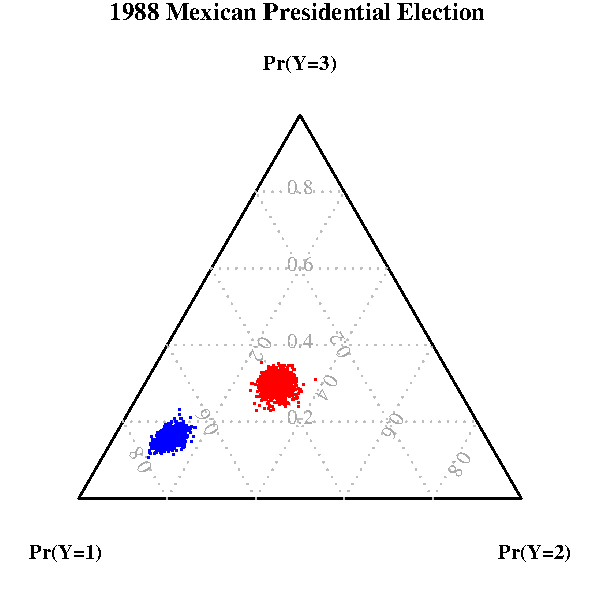
\includegraphics{figs/ternary}
\end{center}

\newpage

\item {\bf ROC Plots} summarize how well models for binary dependent
  variables (logit and probit) fit the data.  The ROC plot
  evaluates the fraction of 0's and 1's correctly predicted for every
  possible threshold value at which the continuous Prob$(Y = 1)$ may
  be realized as a dichotomous prediction.  The closer the ROC curve
  is to the upper right corner of the plot, the better the fit of the
  model specification (King and Zeng, 2002\emph{b})\nocite{KinZen02}.
  See Section \ref{ROC} for the sample code, and type {\tt demo(roc)} at the
  R prompt to run the example.

\begin{center}
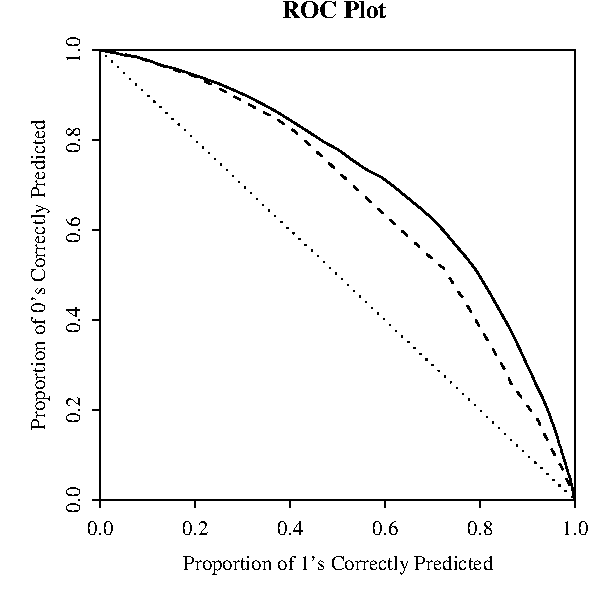
\includegraphics{figs/roc}
\end{center}

\newpage

\item {\bf Vertical Confidence Intervals} may be used for almost any
  model, and describe simulated confidence intervals for any quantity
  of interest while allowing one of the explanatory variables to vary
  over a given range of values (King, Tomz and Wittenberg,
  2000)\nocite{KinTomWit00}. Type {\tt demo(vertci)} at the R prompt to
  run the example, and {\tt help.zelig(plot.ci)} for the manual page.

\begin{center}
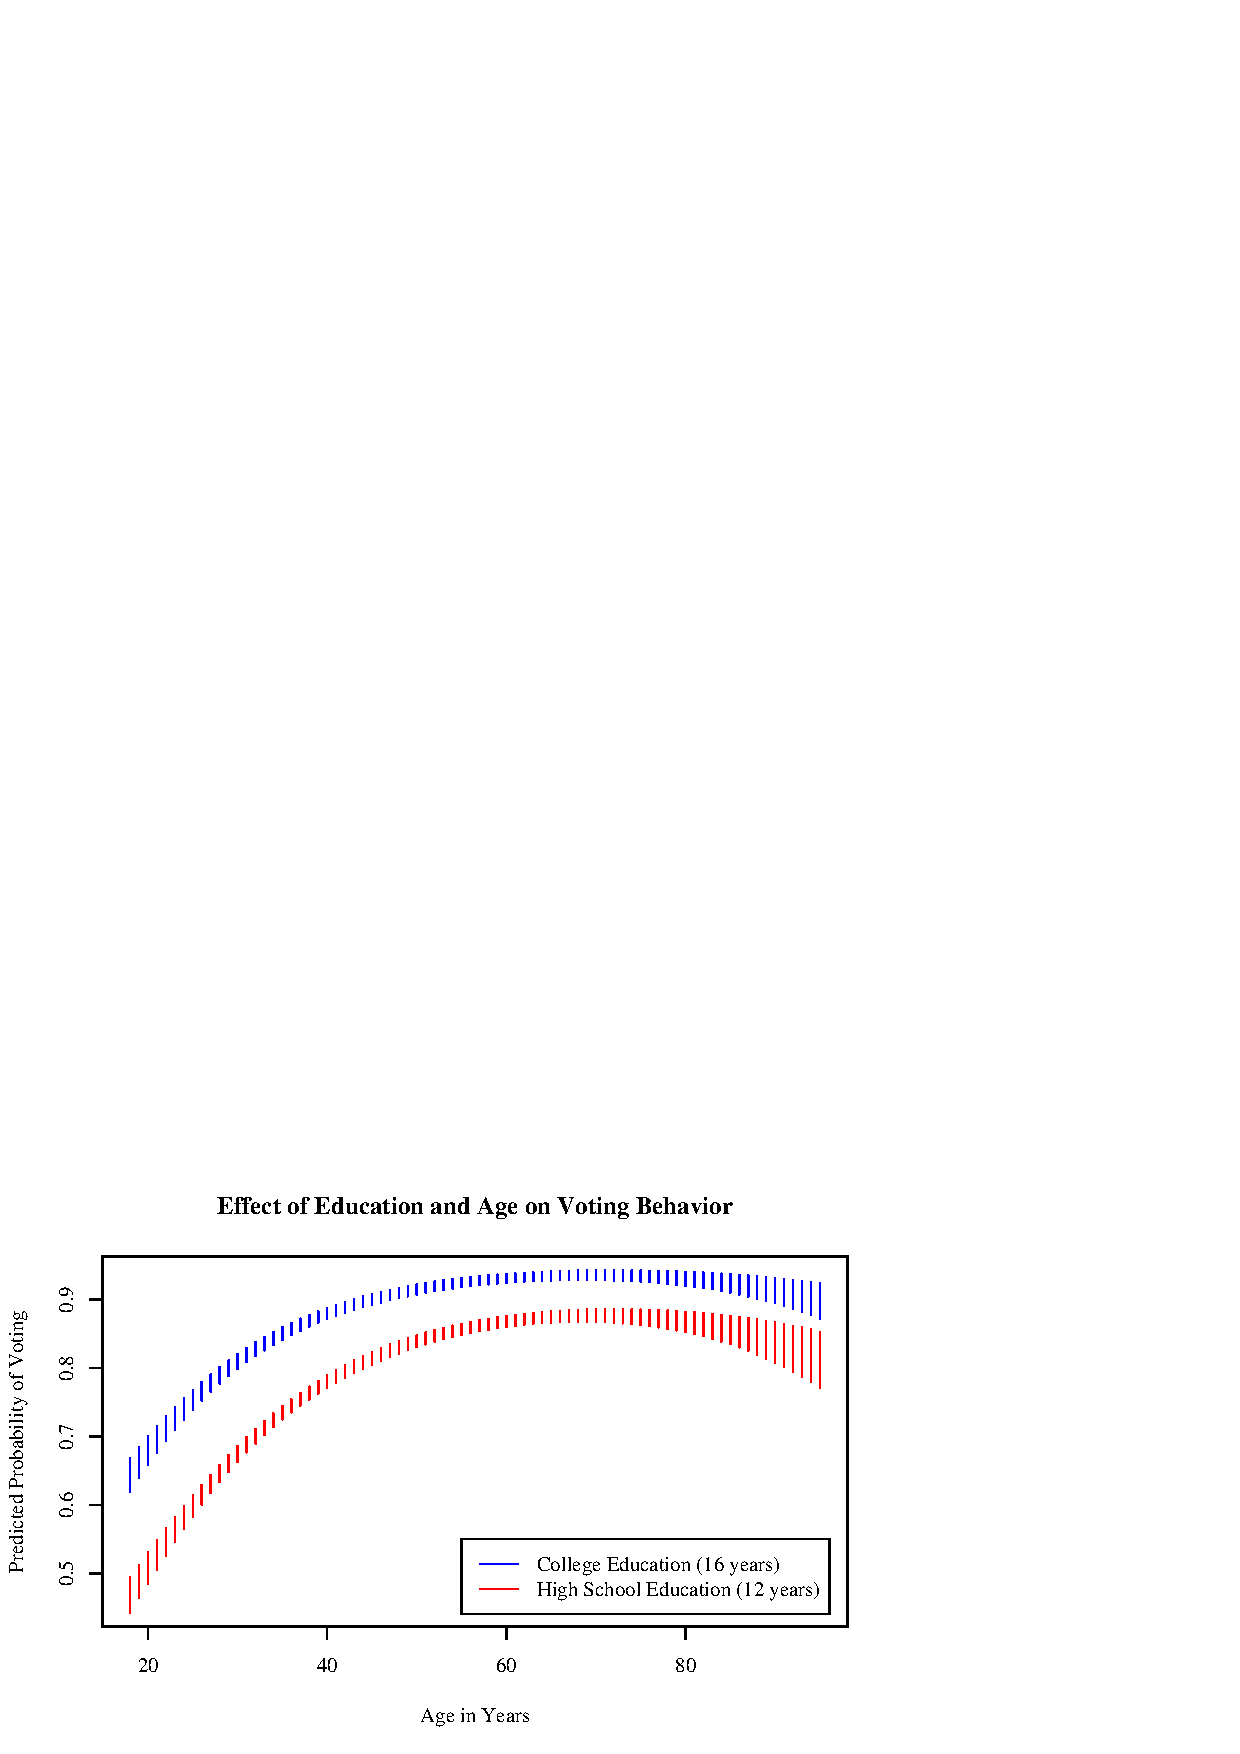
\includegraphics{figs/vertci}
\label{plot.vertci}
\end{center}

\end{enumerate}

%%% Local Variables: 
%%% mode: LaTeX
%%% TeX-master: "zelig"
%%% End:



% Part: ZELIG API
\part{The Zelig Developers' API}
\label{part:The Zelig API}

\chapter[Development Guide]{Rapid Development Guide}
\label{chapter:Quickstart}

% Section: introduction
% Modified:7/6/2011
% By: Matt Owen
% This section gives an introduction to Zelig

\section{Introduction}\label{section:introduction}

Programming a Zelig module is a simple procedure. By following several simple steps, any statistical model can be implemented in the Zelig software suite. The following document places emphasis on speed and practicality, rather than the numerous, technical details involved in developing statistical models. That is, this guide will explain how to quickly and most simply include existing statistical software in the Zelig suite.


% Section: overview
% Modified:7/6/2011
% By: Matt Owen
% This section gives an overview of Zelig's necessary components

\section{Overview}\label{section:overview}

In order for a Zelig model to function correctly, four components need to exist:

\begin{description}

	\item[\emph{a statistical model}:] This can be any statistical model of the developer's choosing, though it is suggested that it be written in R. Examples of statistical models already implemented in Zelig include: Brian Ripley's \code{glm} and Kosuke Imai's \code{MNP} models.

	\item[\code{zelig2}\emph{model}] This method acts as a bridge between the external statistical model and the Zelig software suite

	\item[\code{param.}\emph{model}] This method specifies the simulated parameters used to compute quantities of interest

	\item[\code{qi.}\emph{model}] This method computes - using the fitted statistical model, simulated parameters, and explanatory data - the \emph{quantities of interest}. Compared with the \code{zelig2} and \code{param} methods, 

\end{description}

In the above description, replace the italicized \emph{model} text with the name of the developer's model. For example, if the model's name is ``logit'', then the corresponding methods will be titled \code{zelig2logit}, \code{param.logit}, and \code{qi.logit}.


% Section: zelig.skeleton
% Modified:7/6/2011
% By: Matt Owen
% This section gives details concerning zelig.skeleton

\section{\code{zelig.skeleton}: Automating Zelig Model Creation}\label{zelig.skeleton}

The fastest way to setup and begin programming a Zelig model is the use the \code{zelig.skeleton} function, available within the \code{Zelig} package. This function allows a fast, simple way to create the \code{zelig2}, \code{describe}, \code{param}, and \code{qi} methods with the necessary boilerplate. As a result, \code{zelig.skeleton} closely mirrors the \code{package.skeleton} method included in core R.

\subsection{A Demonstrative Example}

\begin{verbatim}
library(Zelig)  # [1]

zelig.skeleton(
               "my.zelig.package",                # [2]
               models = c("gamma", "logit"),      # [3]
               author = "Your Name",              # [4]
               email = "your.email@someplace.com" # [5]
               )
\end{verbatim}

\subsection{Explanation of the \code{zelig.skeleton} Example}

The above numbered comments correspond to the following:

\begin{description}

	\item[{[1]}] The Zelig package must be imported when using \code{zelig.skeleton}.

	\item[{[2]}] The first parameter of \code{zelig.skeleton} specifies the name of the package

	\item[{[3]}] The \code{models} parameter specifies the titles of the Zelig models to be included in the package. In the above example, all necessary files and methods for building the ``gamma'' and ``logit'' models will be included in Zelig package.

	\item[{[4]}] Specify the author's name

	\item[{[5]}] Specify the email address of the software maintainer

\end{description}

\subsection{Conclusion}

The \code{zelig.skeleton} function provides a way to automatically generate the necessary methods and file to create an arbitrary Zelig package. The method body, however, will be incomplete, save for some light documentation additions and programming boilerplate. For a detailed specification of the \code{zelig.skeleton} method, refer to Zelig help file by typing:

\begin{verbatim}
library(Zelig)

?zelig.skeleton
\end{verbatim}

{\noindent}in an interactive R-session.
 

\section{\emph{zelig2}: Interacting with Existing Statistical Models in Zelig}
\label{section:zelig2}

The \code{zelig2} function acts as the bridge between the Zelig module and the existing statistical model. That is, the results of this function specify the parameters to be passed to a \emph{previously completed} statistical model-fitting function. In this sense, there is nothing tricky about the \code{zelig2} function. Simply construct a list with key-value pairs in the following fashion:

\begin{itemize}

  \item {\bf Keys} (names on the lefthand-side of an equal sign) represent
        parameters that are submitted to the existing model function

  \item {\bf Values} (variables, etc. on the righthand-side of an equal sign)
        represent values to set the corresponding the parameter to.
        
  \item {\bf Keys with leading periods} are typically reserved for specific
        \code{zelig2} purposes. In particular, the key \code{.function}
        specifies the name of the function that calls the existing statistical
        model.
	\item[an ellipsis (\dots)] specifies that all additional, optional parameters not specified in the signature of the \code{zelig2model\_function} method, will be included in the external method's call, despite not being specifically set.


\end{itemize}

\subsection{A Simple Example}

\noindent For example, if a developer wanted to call an existing model
\code{"SomeModel"} with the parameter \code{weights} set to \code{1},
the appropriate return-value (a list) for the \code{zelig2} function would be:


% SHORT EXAMPLE
\begin{verbatim}
zelig2some.model <- function(formula, data) {
    list(.function = "SomeModel",
         formula   = formula,
         weights   = 1
         )
}
\end{verbatim}


% ....
\subsection{A More Detailed Example}

\noindent A more typical example would be the case of fitting a basic logistic
regression. The following code, already implemented in Zelig, acts as an
interface between Zelig packages and R's built-in \code{glm} function:


% LONG EXAMPLE
\begin{verbatim}
zelig2logit <- function (formula, weights = NULL, ..., data) {
  list(.function = "glm",    # [1]
       
       formula = formula,    # [2]
       weights = weights,    # ...
       data    = data,       # ...

       family  =             # [3]
                 binomial(link="logit"),
       model   = FALSE       # ...
       )
}
\end{verbatim}

\noindent The comments in the above code correspond to the following:

\begin{description}
	\item[{[1]}] Pass all parameters to the \code{glm} function

	\item[{[2]}] Specify that the parameters \code{formula}, \code{weights}, and \code{data} be given the same values as those passed into the \code{zelig2} function itself. That is, whichever values the end-user passes to \code{zelig} will be passed to the \code{glm} function

	\item[{[3]}] Specify that the parameters \code{family} and \code{model} \emph{always} be given the corresponding values - \code{binomial(link="logit")} and \code{FALSE} - regardless of what the end-user passes as a parameter.
	
\end{description}

Note that the parameters - \code{formula}, \code{weights}, \code{data}, \code{family}, \code{model} - correspond to those of the \code{glm} function. In general, this will be the case for any \code{zelig2} method. That is, every \code{zelig2} method should return a list containing the parameters belonging to the external model, as well as, the reserved keyword \code{.function}.

If you are unsure about the parameters that are passed to an existing statistical model, simply use the \code{args} or \code{formals} functions (included in R). For example, to get a list of acceptable parameters to the \code{glm} function, simply type:

\begin{verbatim}
args(glm)
\end{verbatim}


\subsection{An Even-More Detailed Example}

{\noindent}Occasionally the statistical model and the standard style of Zelig input differ. In these instances, it may be necessary to manipulate information about the \code{formula} and \code{constraints}. This additional step in building the \code{zelig2} method is common only amongst multivariate models, as seen below in the \code{bprobit} model (bivariate probit regression for Zelig).

% Complex example of a Zelig 2 Function
%

\begin{verbatim}
zelig2bprobit <- function(formula, ..., data) {

  # [1]
  formula <- parse.formula(formula, "bprobit")
  
  # [2]
  tmp <- cmvglm(formula, "bprobit", 3)

  
  # return list
  list(
       .function = "vglm",    # [3]
       
       formula = tmp$formula, # [4]
       family  = bprobit,     # [5]
       data = data,
       # [6]
       constraints = tmp$constraints
       )
}
\end{verbatim}

{\noindent \bf The following is an explanation of the above code:}

% Describe the above code
%

\begin{description}

	\item[{[1]}] Convert Zelig-style \code{formula} data-types into the style that the \code{vglm} function understands

	\item[{[2]}] Extract constraint information from the \code{formula} object, as is the style commonly supported by Zelig

	\item[{[3]}] Specify the \code{vglm} as the statistical model fitting function

	\item[{[4]}] Specify the formula to be used by the \code{vglm} function when performing the model fitting. Note that this object is created by using both the \code{parse\.formula} and \code{cmvglm} functions 

	\item[{[5]}] Specify the \code{family} of the model

	\item[{[6]}] Specify the constraints to be used by the \code{vglm} function when performing the model fitting. Note that this object is created by using both the \code{parse\.formula} and \code{cmvglm} functions

\end{description}

% Explain how to look up information on the cmvglm and parse.formula functions
%

\noindent Note that the functions \code{parse.formula} and \code{cmvglm} are included in the core Zelig software package. Information concerning these functions can be found by typing:

\begin{verbatim}
library(Zelig)

?parase.formula
?cmvglm
\end{verbatim}

in an interactive R-session.


\subsection{Summary and More Information aboput \code{zelig2} Methods}

\code{zelig2} functions can be of varying difficulty - from simple parameter passing to reformatting and creating new data objects to be used by the external model-fitting function. To see more examples of this usage, please refer to the \code{survey.zelig} and \code{multinomial.zelig} packages. Regardless of the model's complexity, it ends with a simple list specifying which parameters to pass to a preexisting statistical model.

For more information on the \code{zelig2} function's full features, see
the \emph{Advanced zelig2 Manual}, or type:

\begin{verbatim}
library(Zelig)

?zelig2
\end{verbatim}

within an interactive R-session.


% Section:  param
% Modified: 6/29/2011
% By: Matt Owen
% This section explains how to use the param API

\section{\emph{param}: Simulating Parameters}\label{section:param}


The \code{param} function simulates and specifies parameters necessary for computing
\emph{quantities of interest}. That is, the \code{param} function is the ideal place
to specify information necessary for the \code{qi} method. This includes:

\begin{description}

	\item[Ancillary parameters] These parameters specifying information about the
		underlying probability distribution. For example, in the case of the Normal
		Distribution, $\sigma$ (standard deviation) and $\mu$ (mean) would be considered ancillary parameters.
	
	\item[Link function] That is, the function providing the relationship between
		the predictors and the mean of the distribution function. This is typically of
		very little importance (compared to the inverse link function), but is frequently included for completeness. For Gamma distribution, the link function is the inverse function: $ f(x) = \frac{1}{x} $
	
	\item[Inverse link function] Typically crucial for simulating \emph{quantities of
		interest} of \emph{Generalized Linear Models}. For the binomial distribution, the inverse-link function is the logit function: $ f(x) = \frac{e^x}{1+e^x} $
	
	\item[Simulated Parameters] These random draws simulate the parameters of the fitted statistical model. Typically, the \code{qi} method uses these to simulate \emph{quantities of interest} for the given model. As a result, these are of paramount importance.

\end{description}

\noindent The following sections describe how these ideas correspond to the structure of a well-written
\code{param} function.

\subsection{The Function Signature}

The \code{param} function takes only two parameters, but outputs a wealth of information important in computing \emph{quantities of interest}. The following is the function signature:

\begin{verbatim}
  param.logit <- function (obj, num)
\end{verbatim}

\noindent The above parameters are:

\begin{description}
	\item[obj] An object of class \code{zelig}
		\footnote{
		%
		%
		For a detailed specification of the \code{zelig} class, type: \code{?zelig} within a interactive Zelig-session.
		}. This contains the fitted statistical model and associated information.	
			
	\item[num] An integer specifying the number of simulations to be drawn. This value is specified by the end-user, and defaults to \code{1000} if no value is specified.

\end{description}

% For full technical documen

\subsection{The Function Return Value}

In similar fashion to the \code{zelig2} method, the \code{param} method takes return values as a list of key-value pairs. However, the options are not as diverse. That is, the list can only be given a set of specific values: \code{ancillary}, \code{coef}, \code{simulations}, \code{link}, \code{linkinv}, and \code{family}.

In most cases, however, the parameters \code{ancillary}, \code{simulations}, and \code{linkinv} are sufficient. The following is an example take from Zelig's \code{gamma} model:

\pagebreak
\begin{verbatim}
# Simulate Parameters for the gamma Model
param.gamma <- function(obj, num) {

# NOTE: gamma.shape is a method belonging to the
#       GLM class, specifying maximum likelihood
#       estimates of the distribution's shape
#       parameter. It is a list containing two
#       values: 'alpha' and 'SE'

  shape <- gamma.shape(obj)
	
  # simulate ancillary parameters
  alpha <- rnorm(n=num, mean=shape$alpha, sd=shape$SE)
  
  # simulate maximum
  sims <- mvrnorm(n = num, mu = coef(obj), Sigma = vcov(obj))

	# return results  
  list(
       alpha = alpha,       # [1]
       simulations  = sims, # [2]
                            # ...
                               
                            # [3]
       linkinv = function (x) 1/x
       )
}

\end{verbatim}

The above code does the following:

\begin{description}

	\item[{[1]}] Specify the ancillary parameters, typically referred to as the greek letter $\alpha$. In the above example, \code{alpha} is the \emph{shape} of the model's underlying gamma distribution.
	
	\item[{[2]}] Specify the parameter simulations, typically referred to as the greek letter $\beta$, to be used in the \code{qi} function.
	
	\item[{[3]}] Specify the inverse-link function
		\footnote{The ``inverse-link'' function is also commonly referred to as the ``mean'' function. Typically, this function specifies the relationship between linear predictors and the mean of a distribution function. As a result, it is only used in describing \emph{generalized linear models} },
		used to compute \emph{expected values} and a variety of other \emph{quantities of interest}, once samples are extracted from the model's statistical distribution.

\end{description}


\subsection{Summary and More Information \code{param} Methods}

The \code{param} method's basic purpose is to describe the statistical and systematic variables of the Zelig model's underlying distribution. Defining this method is an important step towards simplifying the \code{sim} method. That is, by specifying features of the model - coefficients, systematic components, inverse link functions, etc. - and simulating specific parameters, the \code{sim} method can focus entirely on simulating \emph{quantities of interest}.
	


% Section:  qi
% Modified: 6/29/2011
% By: Matt Owen
% This section explains how to use the qi API

\section{qi: Simulating Quantities of Interest}\label{section:qi}

The \code{qi} function of any Zelig model simulates \emph{quantities of interest}
using the fitted statistical model, taken from the \code{zelig2} function,
and the simulated parameters, taken from the \code{param} function. As a result,
the \code{qi} function is the most important component of a Zelig model.

\subsection{The \code{qi} Function Signature}

While the implementation of the \code{qi} function can differ greatly from one
model to another, the signature always remains the same and closely parallels the 
signature of the \code{sim} function.


\begin{verbatim}
qi.logit <- function(obj, x=NULL, x1=NULL, y=NULL, param=NULL)
\end{verbatim}



\subsection{The \code{qi} Function Return Values}

Similar to the return values of both the \code{zelig2} and \code{param} function,
the \code{qi} function takes an list of key-value pairs as a return value. The keys,
however, follow a much simpler convention, and a single rule: the key (left-side
of the equal sign) is a \emph{quoted} character-string naming the \emph{quantity of
interest} and the value (right-side of the equal sign) are the actual simulations.

The following is a short example:

\begin{verbatim}
  list(
       "Expected Value"  = ev,
       "Predicted Value" = pv
       )
\end{verbatim}

\noindent where \code{ev} and \code{pv} are respectively simulations of the model's
\emph{expected values} and \emph{predicted values}.

\subsection{Coding Conventions for the \code{qi} Function}

While the following is unnecessary, it provides a few simple guidelines to simplifying
and improving readability of a model's \code{qi} function:

\begin{itemize}

	\item Divide repetitive work amongst other functions. For example, if you simulate
		an \emph{expected value} for both the \code{x} and \code{x1}, it is better to 
		write a \code{.compute.ev} function and simply call it twice
		
	\item Always compute an \emph{expected values} and \emph{predicted values} independently
		and before writing code to create \emph{first differences}, \emph{risk ratios}, and
		\emph{average treatment effects}
		
	\item Write code for \emph{average treatment effects} only after all the other code has
		been debugged and completed

\end{itemize}

\pagebreak
\subsection{A Simplified Example}

The following is a simplified example of the \code{qi} function for the logit model. Note that the example is divided into two sections: one specifying the return values and titles of the \emph{quantities of interest} (see Section~\ref{example:qi.logit}) and one computing the simulated \emph{expected values} of the model (see Section~\ref{example:.compute.ev}).


\subsubsection{\code{qi.logit} Function}\label{example:qi.logit}
\begin{verbatim}
#' simulate quantities of interest for the logit models
qi.logit <- function(obj, x=NULL, x1=NULL, y=NULL, num=1000,
                     param=NULL) {
  # [1]
  ev1 <- .compute.ev(obj, x, num, param)
  ev2 <- .compute.ev(obj, x1, num, param)

  # [2]
  list(
       "Expected Values: E(Y|X)"  = ev1,
       "Expected Values (for X1)" = ev2,
       
  # [3]
       "First Differences: E(Y|X1) - E(Y|X)" = ev2 - ev1
       )
}
\end{verbatim}


\subsubsection{\code{.compute.ev} Function}\label{example:.compute.ev}
\begin{verbatim}
.compute.ev <- function(obj, x=NULL, num=1000, param=NULL) {
  # values of NA are ignored by the summary function
  if (is.null(x))
    return(NA)

  # extract simulations
  coef <- coef(param)
  
  link.inverse <- linkinv(param)

  eta <- coef %*% t(x)

  # invert link function
  theta <- matrix(link.inverse(eta), nrow = nrow(coef))
  ev <- matrix(theta, ncol=ncol(theta))

  ev
}  
\end{verbatim}

\noindent The above code illustrates a few of the ideas:

\begin{description}

	\item[{[1]}] Compute \emph{quantities of interest} using re-usable functions that express the idea clearly. This both reduces the amount of code necessary to produce the simulations, and improves readability of the source code.
	
	\item[{[2]}] Return \emph{quantities of interest} as a list. Note: titles of
		\emph{quantities of interest} are on the left of the equal signs, while
		simulated values are on the right.
		
	\item[{[3]}] Simulate \emph{first differences} by using two previous computed \emph{quantities of interest}.
	  
	\item[{[4]}] Define an additional function that simulates \emph{expected values}, rather than placing such code in the actual \code{qi} method.

\end{description}

\noindent In addition, this function two \emph{generic functions} that are
defined in the Zelig software suite, and are particularly used with the \code{param} class:

\begin{description}

	\item[coef] Extract the simulations of the parameters. Specifically, this returns the simulations produced in the \code{param} function
	
	\item[linkinv] Return the inverse of the link function. Specifically, this returns the inverse-link functions specified in the \code{param} function

\end{description}

\subsection{Summary and More Information about \code{qi} Methods}

The \code{qi} function offers a simple template for computing \emph{quantities of interest}. Particularly, if a few a coding conventions are followed, the \code{qi} function can provide transparent, easy-to-read simulation methods.

\section{Conclusion}

The above sections detail the fastest way to develop Zelig models. For the vast majority of applications and external statistical packages, this should suffice. However, at times, more elaborate measures may need to be taken. If this is the case, the API specifications for each particular methods should be read, since a wealth of information has been omitted in order to simplify this tutorial.

For more detailed information, consult the \code{zelig2}, \code{param}, and \code{qi} sections of the Zelig Development manual.


\chapter[zelig2]{zelig2: Interfacing External Methods with Zelig}
\label{chapter:Zelig2}
\documentclass[11pt]{article}
\usepackage{ZeligDoc}
\begin{document}

% TITLE INFORMATION
\title{Making the Model Compatible with Zelig: Writing the \emph{zelig2} Function}
\author{Matthew Owen}
\maketitle


% INTRODUCTION
\section{Introduction}
Developers can develop a model, write the model-fitting function, and test it
within the Zelig framework without explicit intervention from the Zelig team. 
This modularity relies on two R programming conventions:


\begin{enumerate}

	\item {\bf wrappers}, which pass arguments from R functions to other R functions
		or foreign function calls (such as in C, C++, or Fortran).  This step is
		facilitated by - as will be explained in detail in the upcoming chapter -
		the {\tt zelig2} function.
		
	\item {\bf classes}, which tell generic functions how to handle objects of a given
		class.  For a statistical model to be compliant with Zelig, the model-fitting
		function \emph{must} return a classed object.
		
\end{enumerate}

Zelig implements a unique and simple method for incorporating existing statistical
models which lets developers test \emph{within} the Zelig framework \emph{without} any
modification of both their own code or the {\tt zelig} function itself.  The heart of
this procedure is the {\tt zelig2} function, which acts as an interface between the
{\tt zelig} function and the existing statistical model.  That is, the {\tt zelig2}
function maps the user-input from the {\tt zelig} function into input for the existing
statistical model's constructor function.  Specifically, a Zelig model requires:

% !!
%
\begin{enumerate}

	\item An existing statistical model, which is invoked through a function call and
		returns an object

	\item A {\tt zelig2} function which maps user-input from the {\tt zelig} function to
		the existing statistical model
		
	\item A name for the {\tt \bf zelig} model, which can differ from the original name of
		the statistical model.
		
\end{enumerate}


% THE ZELIG2 FUNCTION
\section{The \emph{zelig2} Function}
The following sections explain how to write a {\tt zelig2} function, given an arbitrary
statistical model.  In the illustrative examples, the following conventions are used:



\begin{description}

	\item[model] will refer to the name of the \emph{Zelig} model, not the name of the
		existing model - though these two names are not necessarily different.  If the developer
		names his model ``logit'' then model refers to ``logit''.

	\item[model\_function] will refer to the name of function that produces the existing
		statistical model.  If the developer is writing a wrapper for R's built-in logit function,
		then \emph{model\_function} refers to ``glm''.
		
	\item[zelig2model] will refer to the name of the {\tt zelig2} function.  If the developer
		names his model ``logit'', then \emph{zelig2model} refers to ``zelig2logit''.
		
\end{description}


% WRITING THE ZELIG2 FUNCTION
\subsection{Writing the \emph{zelig2} Function}

The {\tt zelig2} function should follow several specific conventions:

\begin{enumerate}

	\item The {\tt zelig2model} function should be simply named \emph{zelig2model}, where
		\emph{model} is the chosen name for the zelig package

	\item The {\tt zelig2model} function itself should have arguments that list entirety of
		possible inputs to the {\tt model\_function}

	\item The {\tt zelig2model} function should return a list of key-value pairs that represent
		the map from {\tt zelig} input to {\tt model\_function} input

\end{enumerate}


% EXAMPLE USING zelig2logit
\pagebreak
\subsection{Example of a \emph{zelig2} Function}

\begin{verbatim}
zelig2logit <- function(formula, ..., data, weights=NULL)
  list(
       .function = "glm",
        
       formula = formula,
       data    = data,
       weights = weights,
        
       family = binomial(link="logit"),
       model  = FALSE
       )
\end{verbatim}


% EXPLANATION
\subsection{Explanation of \code{zelig2} Return Values}

A {\tt zelig2model} function must always return a list as its return value.

The entries of the returned list have the following format:

\begin{description}

	\item[\code{.function}] specifies, with a character string, {\tt model\_function} used to fit the data
	
	\item[key-value pairs] represent an explicit mapping specified by the developer for the
		parameter that matches ``key''. Value are specified typically in one of two ways:

		\begin{itemize}
		
			\item As a variable based on some information from the user. In the above example, this
				corresponds to the \code{formula}, \code{data}, and \code{weights} keys in the returned
				list. \emph{Note how all the parameters make use of variables specified in the function
				signature}

			\item As a variable that is statically set. This is useful for parameters that do not require
				user-input. In the above example, this corresponds to the \code{family} and \code{model}
				parameters, as their values are specified to specific values regardless of user-input.
				\emph{Note how neither parameter make no use of the parameters in the function signature}
						
		\end{itemize}
	
	\item[an ellipsis (\dots)] specifies that all additional, optional parameters not specified in the signature of the \code{zelig2model\_function} method, will be included in the external method's call, despite not being specifically set.
				
	
\end{description}


\end{document}
























\chapter[param]{param:Generalizing Common Components of Fitted Statistical Models}
\label{chapter:Parameters}
\section{Introduction}
\label{section:param-intro}

Several general features - sampling distribution, link function,
systematic component, ancillary parameters, etc. - comprise
statistical models.  These features, while vastly differing between
any two given specific models, share features that are easily
classifiable, and usually necessary in the simulation of
\emph{quantities of interest}.  That is, all statistical models have
similar traits, and can be simulated using similar methods.  Using
this fact, the \emph{parameters} class provides a set of functions
and data-structures to aid in the planning and implementation of 
the statistical model.

\section{Method Signature of \code{param}}

The signature of the \code{param} method is straightforward and does not vary between differ Zelig models.

\begin{Code}
param.logit <- function (obj, num, ...) {
  # ...
}
\end{Code}

\section{Return Value of \code{param}}

The return value of a \code{param} method is simply a list containing several entries:

\begin{description}
	\item[simulations] A vector or matrix of random draws taken from
		the model's distribution function.  For example, a logit model
		will take random draws from a Multivariate Normal distribution.
		
	\item[alpha] A vector specifying parameters to be passed into
		the distribution function.  Values for this range from scaling
		factors to statistical means.
	
	\item[fam] An optional parameter.  \emph{fam} must be an object
		of class ``family''.  This allows for the implicit specification
		of the link and link-inverse function.  It is recommend that the
		developer set either this, the link, or the linkinv parameter
		explicitly.  Setting the family object implicitly defines
		\emph{link} and \emph{linkinv}.
		
	\item[link] An optional parameter.  \emph{link} must be a function.
		Setting the link function explicitly is useful for defining
		arbitrary statistical models.  \emph{link} is used primarily to
		numerically approximate its inverse - a necessary step for
		simulating \emph{quantities of interest}.
		
	\item[linkinv] An optional parameter.  \emph{linkinv} must be a
		function.  Setting the link's inverse explicitly allows for faster
		computations than a numerical approximation provides.  If the
		inverse function is known, it is recommended that this function
		is explicitly defined.
		
\end{description}

%\section{Methods of the \code{parameters} Object}
%\begin{description}
%	\item[alpha] Extracts the contents of alpha
%	\item[coef] Extracts the simulated parameters specified in the key \code{simulations}
%	\item[link] Extracts the link function from the parameter.  This value exists as long as \emph{fam} or \emph{link} are explicitly set
%	\item[linkinv] Extracts the link-inverse function from the parameters. This value exists as long as \emph{fam}, \emph{link} or \emph{linkinv} are explicitly set.  If \emph{linkinv} is not explicitly set, then a numerical approximation is used based on \emph{fam} or \emph{link}
%\end{description}


\section{Writing the \emph{param} Method}

The ``param'' function of an arbitrary Zelig model draws samples from the
model, and describes the statistical model.  In practice, this may be done
in a variety of fashions, depending upon the complexity of the model


% LIST METHODS
% ------------
% LOGIT EXAMPLE
\subsection{List Method: Returning an Indexed List of Parameters}

While the simple method of returning a vector or matrix from a \emph{param} function is extremely simple, it has no method for setting link or link-inverse functions for use within the actual simulation process.  That is, it does not provide a clear, easy-to-read method for simulating \emph{quantities of interest}.  By returning an indexed list - or a parameters object - the developer can provide clearly labeled and stored link and link-inverse functions, as well as, ancillary parameters.


\subsubsection{Example of Indexed List Method with \emph{fam} Object Set}

\begin{verbatim}
param.logit <- function(z, x, x1=NULL, num=num)
  list(
       coef  = mvrnorm(n=num, mu=coef(z), Sigma=vcov(z)),
       alpha = NULL,
       fam   = binomial(link="logit")
       )
\end{verbatim}

% warum kommst du nicht herueber?

\subsubsection{Explanation of Indexed List with \emph{fam} Object Set Example}

The above example shows how link and link-inverse functions (for a ``logit'' model) can be set using a ``family'' object.  Family objects exist for most statistical models - logit, probit, normal, Gaussian, et cetera - and come preset with values for link and link-inverses.  This method does not differ immensely from the simple, vector-only method; however, it allows for the use of several API functions - \emph{link}, \emph{linkinv}, \emph{coef}, \emph{alpha} - that improve the readability and simplicity of the model's implementation.

The \emph{param} function and the \emph{parameters} class offer methods for automating and simplifying a large amount of repetitive and cumbersome code that may come with building the arbitrary statistical model.  While both are in principle entirely optional - so long as the \emph{qi} function is well-written - they serve as a means to quickly and elegantly implement Zelig models.


% POISSON EXAMPLE
\subsubsection{Example of Indexed List Method (with \emph{link} Function) Set}

\begin{verbatim}
param.poisson <- function(z, x, x1=NULL, num=num) {
  list(
       coef = mvrnorm(n=num, mu=coef(z), Sigma=vcov(z)),
       link = log,
             
       # because ``link'' is set,
       # the next line is purely optional
       linkinv = exp
       )
}
\end{verbatim}

\subsubsection{Explanation of Indexed List (with \emph{link} Function) Example}

The above example shows how a \emph{parameters} object can be created with by explicitly setting the statistical model's link function.  The \emph{linkinv} parameter is purely optional, since Zelig will create a numerical inverse if it is undefined.  However, the computation of the inverse is typically slower than non-iterative methods.  As a result of this, if the link-inverse is known, it should be set, using the \emph{linkinv} parameter.

The above example can also contain an \emph{alpha} parameter, in order to store important ancillary parameters - mean, standard deviation, gamma-scale, etc. - that would be necessary in the computation of \emph{quantities of interest}.


%
\section{Using a \emph{parameters} Object}

Typically, a \emph{parameters} object is used within a model's \emph{qi} function.  While the developer can typically omit the \emph{param} function and the \emph{parameters} object, it is not recommended.  This is because making use of this function can vastly improve readability and functionality of a Zelig model.  That is, \emph{param} and \emph{parameters} automate a large amount of repetitive, cumbersome code, and offer allow access to an easy-to-use API.

\subsection{Example \emph{param} Function}

\begin{Code}
qi.logit <- function(z, x, x1=NULL, sim.param=NULL, num=1000) {
  coef <- coef(sim.param)
  inverse <- linkinv(sim.param)

  eta <- coef %*% t(x)
  theta <- link.inverse(eta)

  # et cetera...
}

\end{Code}


\subsection{Explanation of Above \emph{qi} Code}

The above is a portion of the actual code used to simulate \emph{quantities of interest} for a ``logit'' model.  By using the sim.par object, which is automatically passed into the function if a \emph{param} function is written, \emph{quantities of interest} can be computed extremely generically.  The step-by-step process of the above function is as follows:

\begin{itemize}
	\item{Assign the simulations from \emph{param.logit} to the variable ``coef''}
	\item{Assign the link-inverse from \emph{param.logit} to the variable ``inverse''}
	\item{Compute $\eta$ (eta) by matrix-multiplying our simulations with our explanatory results}
	\item{Conclude ``simulating'' the \emph{quantities of interest} by applying the inverse of the link function.  The result is a vector whose median is an approximate value of the \emph{quantity of interest} and has a standard deviation that will define the confidence interval around this value}
	
\end{itemize}


\section{Future Improvements}

In future releases of Zelig, \emph{parameters} will have more API functions to facilitate common operations - sample drawing, matrix-multiplication, et cetera - so that the developer's focus can be exclusively on implementing important components of the model.

\chapter[qi]{qi: Simulating Quantities of Interest}
\label{chapter:Qi}
\section{Introduction}
% Introduction Material

For any Zelig module, the \emph{qi} function is ultimately the most
important piece of code that must be written; it describes the actual
process which simulates the \emph{quantities of interest}.  Because of
the nature of this process - and the gamut of statistical packages and
their underlying statistical model - it is rare that the simulation
process can be generalized for arbitrary fitted models.  Despite this,
it is possible to break down the simulation process into smaller steps.


%
%
\section{Notable Features of \emph{qi} Function}

The typical \emph{qi} function has several basic procedures:

\begin{enumerate}

	\item \emph{Call the param function}:  This is entirely optional but
		sometimes important for the clarity of your algorithm.  This step
		typically consists of taking random draws from the fitted model's
		underlying probability distribution.
		
	\item \emph{Compute the Quantity of Interest}: Depending on your model,
		there are several ways to compute necessary quantities of interest.
		Typical methods for computing quantities of interest include:
		\begin{enumerate}
			
			\item Using the sample provided by `param' to generate simulations
				of the \emph{quantities of interest}
			
			\item Using a Maximum-likelihood estimate on the fitted model
			
		\end{enumerate}
		
	\item \emph{Create a list of titles for your Quantities of Interest}: 
	
	\item \emph{Generate the Quantity of Interest Object}: Finally, with the
		computed Quantities of Interest, you must
		
\end{enumerate}


%
\section{Basic Layout of a \emph{qi} Function}
Now with the general outline of a \emph{qi} function defined, it is
important to discuss the expected procedures and specifics of
implementation.


\subsection{The Function's Signature}
% quick intro
The \emph{qi} function's signature accepts 4 parameters:


%
%
\begin{description}

	\item[obj:] An object of type \code{zelig}.  This wraps the fitted
		model in the slot ``result''
		
	\item[x:] An object of type \code{setx}.  This object is used to compute
		important coefficients, parameters, and features of the data.frame passed to
		the function call

	\item[x1:] Also an object of type ``\emph{setx}''.  This object is used in a
		similar fashion, however its presence allows a variety of \emph{quantities
		of interest} to be computed.  Notably, this is a necessary parameter to
		compute first-differences
	
	\item[num:] The number of simulations to compute

	\item[param:] An object of type \code{param}. This is the resulting object from
		the \code{param} function, typically containing a variety of important quantities
		- \code{simulations}, the \code{inverse link function}, \code{}

\end{description}


% code example
%
\subsection{Code Example: \emph{qi} Function Signature}
\begin{verbatim}
qi.your_model_name <- function(z, x=NULL, x1=NULL, num=1000) {
	# start typing your code here
	# ...
	# ...
\end{verbatim}


\noindent Note: In the above example, the function name ``qi.your\_model\_name'' is
merely a placeholder.  In order to register a \emph{qi} function with zelig, the
developer must follow the naming convention qi.\emph{your mode name}, where
\emph{your\_model\_name} is the name of the developer's module.  For example, if a
developer titled his or her zelig module ``logit'', then the corresponding \emph{qi}
function is titled ``\emph{qi.logit}''.

%
\subsection{The Function Body}
The function body of \emph{qi} function varies largely from model to model.  As a
result, it is impossible to create general guidelines to simulate \emph{quantities of
interest} - or even determine what the \emph{quantity of interest} is.  Typical methods
for computing \emph{quantities of interest} include:

\begin{itemize}

	\item Implementing sampling algorithms based on the underlying fitted model, or

	\item ``Predicting'' a large number of values from the fitted model

\end{itemize}


% return values
\subsection{The Return Value}
In order for Zelig to process the simulations, they must be returned in one of several formats:

\begin{itemize}
	% First Example
	\item \begin{Code}
		list(
		     "TITLE OF QI 1" = val1,
		     "TITLE OF QI 2" = val2,
		     # any number of title-val pairs
		     # ...
		     "TITLE OF QI N" = val.n
		     )
	\end{Code}

	% Second Example
	\item \begin{verbatim}
		make.qi(
		        titles = list(title1, title2),
		        stats  = list(val1, val2)
		        )
	\end{verbatim}
  \item
\end{itemize}


In the above example,\emph{val1, val2}are data.frames, matrices, or lists representing
the simulations of the \emph{quantities of interests}, and \emph{title1, title2} - and
any number of titles - are character-strings that will act as human-readable descriptions
of the \emph{quantities of interest}.  Once results are returned in this format, Zelig
will convert the results into a machine-readable format and summarize the simulations
into a comprehensible format.

NOTE: Because of its readability, it is suggested that the first method is used when
returning \emph{quantities of interest}.

% break
\pagebreak


% find better way to output this data
\section{Simple Example \code{qi} function (\code{qi.logit.R})}


\begin{verbatim}
#' simulate quantities of interest for the logit models
qi.logit <- function(z, x=NULL, x1=NULL, y=NULL, num=1000, param=NULL) {

  # compute expected values using the function ".compute.ev"
  ev1 <- .compute.ev(obj, x, num, param)
  ev2 <- .compute.ev(obj, x1, num, param)

  # return simulations of quantities of interest
  list(
       "Expected Values: E(Y|X)"  = ev1,
       "Expected Values (for X1): E(Y|X1)" = ev2,
       "First Differences: E(Y|X1) - E(Y|X)" = ev2 - ev1
       )
}
\end{verbatim}


% Part: Reference Manual
\part{Zelig Reference Manual}
\label{part:Zelig Reference Manual}

% CORE PACKAGES
\chapter[gamma]{gamma: Gamma Regression for Continuous, Positive Dependent Variables}
\label{chapter:Gamma}





\section{{\tt gamma}: Gamma Regression for Continuous, Positive Dependent Variables}\label{gamma}

Use the gamma regression model if you have a positive-valued dependent
variable such as the number of years a parliamentary cabinet endures,
or the seconds you can stay airborne while jumping.  The gamma
distribution assumes that all waiting times are complete by the end
of the study (censoring is not allowed).

\subsubsection{Syntax}

\begin{verbatim}
> z.out <- zelig(Y ~ X1 + X2, model = "gamma", data = mydata)
> x.out <- setx(z.out)
> s.out <- sim(z.out, x = x.out, x1 = NULL)
\end{verbatim}

\subsubsection{Additional Inputs} 

In addition to the standard inputs, {\tt zelig()} takes the following
additional options for gamma regression:  
\begin{itemize}
\item {\tt robust}: defaults to {\tt FALSE}.  If {\tt TRUE} is
selected, {\tt zelig()} computes robust standard errors via the {\tt
sandwich} package (see \cite{Zeileis04}).  The default type of robust
standard error is heteroskedastic and autocorrelation consistent (HAC),
and assumes that observations are ordered by time index.

In addition, {\tt robust} may be a list with the following options:  
\begin{itemize}
\item {\tt method}:  Choose from 
\begin{itemize}
\item {\tt "vcovHAC"}: (default if {\tt robust = TRUE}) HAC standard
errors. 
\item {\tt "kernHAC"}: HAC standard errors using the
weights given in \cite{Andrews91}. 
\item {\tt "weave"}: HAC standard errors using the
weights given in \cite{LumHea99}.  
\end{itemize}  
\item {\tt order.by}: defaults to {\tt NULL} (the observations are
chronologically ordered as in the original data).  Optionally, you may
specify a vector of weights (either as {\tt order.by = z}, where {\tt
z} exists outside the data frame; or as {\tt order.by = \~{}z}, where
{\tt z} is a variable in the data frame).  The observations are
chronologically ordered by the size of {\tt z}.
\item {\tt \dots}:  additional options passed to the functions 
specified in {\tt method}.   See the {\tt sandwich} library and
\cite{Zeileis04} for more options.   
\end{itemize}
\end{itemize}

\subsubsection{Example}

Attach the sample data: 
\begin{Schunk}
\begin{Sinput}
> data(coalition)
\end{Sinput}
\end{Schunk}
Estimate the model: 
\begin{Schunk}
\begin{Sinput}
> z.out <- zelig(duration ~ fract + numst2, model = "gamma", data = coalition)
\end{Sinput}
\begin{Soutput}
How to cite this model in Zelig:
  Kosuke Imai, Gary King, and Olivia Lau. 2011.
  "gamma: Gamma Regression for Continuous, Positive Dependent Variables"
  in Kosuke Imai, Gary King, and Olivia Lau, "Zelig: Everyone's Statistical Software,"
  http://gking.harvard.edu/zelig
\end{Soutput}
\end{Schunk}
View the regression output:  
\begin{Schunk}
\begin{Sinput}
> summary(z.out)
\end{Sinput}
\begin{Soutput}
Call:
glm(formula = duration ~ fract + numst2, family = Function, data = Data.frame, 
    model = FALSE)

Deviance Residuals: 
    Min       1Q   Median       3Q      Max  
-2.2510  -0.9112  -0.2278   0.4132   1.5360  

Coefficients:
              Estimate Std. Error t value Pr(>|t|)    
(Intercept) -1.296e-02  1.329e-02  -0.975  0.33016    
fract        1.149e-04  1.723e-05   6.668 1.19e-10 ***
numst2      -1.739e-02  5.881e-03  -2.957  0.00335 ** 
---
Signif. codes:  0 ‘***’ 0.001 ‘**’ 0.01 ‘*’ 0.05 ‘.’ 0.1 ‘ ’ 1 

(Dispersion parameter for Gamma family taken to be 0.6291004)

    Null deviance: 300.74  on 313  degrees of freedom
Residual deviance: 272.19  on 311  degrees of freedom
AIC: 2428.1

Number of Fisher Scoring iterations: 6
\end{Soutput}
\end{Schunk}
Set the baseline values (with the ruling coalition in the minority)
and the alternative values (with the ruling coalition in the majority)
for X:
\begin{Schunk}
\begin{Sinput}
> x.low <- setx(z.out, numst2 = 0)
> x.high <- setx(z.out, numst2 = 1)
\end{Sinput}
\end{Schunk}
Simulate expected values ({\tt qi\$ev}) and first differences ({\tt qi\$fd}):
\begin{Schunk}
\begin{Sinput}
> s.out <- sim(z.out, x = x.low, x1 = x.high)
\end{Sinput}
\end{Schunk}
\begin{Schunk}
\begin{Sinput}
> summary(s.out)
\end{Sinput}
\begin{Soutput}
Model:  gamma 
Number of simulations:  1000 

Values of X
     fract numst2
1 718.8121      0

Values of X1
     fract numst2
1 718.8121      1


Expected Values: E(Y|X) 
  mean    sd    50%   2.5% 97.5%
 14.47 1.069 14.401 12.577 16.73

Expected Values (for X1): E(Y|X1) 
   mean    sd    50%   2.5%  97.5%
 19.221 1.105 19.201 17.193 21.495

Predicted Values: Y|X 
   mean     sd    50%  2.5%  97.5%
 14.488 13.356 10.896 0.609 50.562

Predicted Values: Y|X1 
   mean     sd    50%  2.5%  97.5%
 19.198 16.407 14.441 1.266 62.279

First Differences: E(Y|X1) - E(Y|X) 
  mean    sd   50%  2.5% 97.5%
 4.751 1.526 4.716 2.001 7.759
\end{Soutput}
\end{Schunk}
\begin{center}
\begin{Schunk}
\begin{Sinput}
> plot(s.out)
\end{Sinput}
\end{Schunk}
\includegraphics{vigpics/gamma-ExamplePlot}
\end{center}

\subsubsection{Model}

\begin{itemize}
\item The Gamma distribution with scale parameter $\alpha$ has a
\emph{stochastic component}:
\begin{eqnarray*}
Y &\sim& \textrm{Gamma}(y_i \mid \lambda_i, \alpha) \\
f(y)  &=& \frac{1}{\alpha^{\lambda_i} \, \Gamma \lambda_i} \, y_i^{\lambda_i
  - 1} \exp -\left\{ \frac{y_i}{\alpha} \right\}
\end{eqnarray*}
for $\alpha, \lambda_i, y_i > 0$.  \\

\item The \emph{systematic component} is given by
\begin{equation*}
  \lambda_i = \frac{1}{x_i \beta}
\end{equation*}
\end{itemize}

\subsubsection{Quantities of Interest}

\begin{itemize}
\item The expected values ({\tt qi\$ev}) are simulations of the mean
  of the stochastic component given draws of $\alpha$ and
  $\beta$ from their posteriors:  $$E(Y) = \alpha \lambda_i.$$  
\item The predicted values ({\tt qi\$pr}) are draws from the gamma
  distribution for each given set of parameters $(\alpha, \lambda_i)$.
\item If {\tt x1} is specified, {\tt sim()} also returns the
  differences in the expected values ({\tt qi\$fd}), $$E(Y \mid x_1) -
  E(Y \mid x)$$.

\item In conditional prediction models, the average expected treatment
  effect ({\tt att.ev}) for the treatment group is 
    \begin{equation*} \frac{1}{\sum_{i=1}^n t_i}\sum_{i:t_i=1}^n \left\{ Y_i(t_i=1) -
      E[Y_i(t_i=0)] \right\},
    \end{equation*} 
    where $t_i$ is a binary explanatory variable defining the treatment
    ($t_i=1$) and control ($t_i=0$) groups.  Variation in the
    simulations are due to uncertainty in simulating $E[Y_i(t_i=0)]$,
    the counterfactual expected value of $Y_i$ for observations in the
    treatment group, under the assumption that everything stays the
    same except that the treatment indicator is switched to $t_i=0$.

\item In conditional prediction models, the average predicted treatment
  effect ({\tt att.pr}) for the treatment group is 
    \begin{equation*} \frac{1}{\sum_{i=1}^n t_i}\sum_{i:t_i=1}^n \left\{ Y_i(t_i=1) -
      \widehat{Y_i(t_i=0)} \right\},
    \end{equation*} 
    where $t_i$ is a binary explanatory variable defining the treatment
    ($t_i=1$) and control ($t_i=0$) groups.  Variation in the
    simulations are due to uncertainty in simulating
    $\widehat{Y_i(t_i=0)}$, the counterfactual predicted value of
    $Y_i$ for observations in the treatment group, under the
    assumption that everything stays the same except that the
    treatment indicator is switched to $t_i=0$.  

\end{itemize}

\subsubsection{Output Values}

The output of each Zelig command contains useful information which you
may view.  For example, if you run \texttt{z.out <- zelig(y \~\,
  x, model = "gamma", data)}, then you may examine the available
information in \texttt{z.out} by using \texttt{names(z.out)},
see the {\tt coefficients} by using {\tt z.out\$coefficients}, and
a default summary of information through \texttt{summary(z.out)}.
Other elements available through the {\tt \$} operator are listed
below.

\begin{itemize}
\item From the {\tt zelig()} output object {\tt z.out}, you may
  extract:
   \begin{itemize}
   \item {\tt coefficients}: parameter estimates for the explanatory
     variables.
   \item {\tt residuals}: the working residuals in the final iteration
     of the IWLS fit.
   \item {\tt fitted.values}: the vector of fitted values.
   \item {\tt linear.predictors}: the vector of $x_{i}\beta$.
   \item {\tt aic}: Akaike's Information Criterion (minus twice the
     maximized log-likelihood plus twice the number of coefficients).
   \item {\tt df.residual}: the residual degrees of freedom.
   \item {\tt df.null}: the residual degrees of freedom for the null
     model.
   \item {\tt zelig.data}: the input data frame if {\tt save.data = TRUE}.  
   \end{itemize}

\item From {\tt summary(z.out)}, you may extract: 
   \begin{itemize}
   \item {\tt coefficients}: the parameter estimates with their
     associated standard errors, $p$-values, and $t$-statistics.
   \item{\tt cov.scaled}: a $k \times k$ matrix of scaled covariances.
   \item{\tt cov.unscaled}: a $k \times k$ matrix of unscaled
     covariances.  
   \end{itemize}

\item From the {\tt sim()} output object {\tt s.out}, you may extract
  quantities of interest arranged as matrices indexed by simulation
  $\times$ {\tt x}-observation (for more than one {\tt x}-observation).
  Available quantities are:

   \begin{itemize}
   \item {\tt qi\$ev}: the simulated expected values for the specified
     values of {\tt x}.
   \item {\tt qi\$pr}: the simulated predicted values drawn from a
     distribution defined by $(\alpha, \lambda_i)$.
   \item {\tt qi\$fd}: the simulated first difference in the expected
     values for the specified values in {\tt x} and {\tt x1}.
   \item {\tt qi\$att.ev}: the simulated average expected treatment
     effect for the treated from conditional prediction models.  
   \item {\tt qi\$att.pr}: the simulated average predicted treatment
     effect for the treated from conditional prediction models.  
   \end{itemize}

\end{itemize}


\subsection*{How to Cite the Gamma Model}
\bibentry{ImaLauKin-logit11}

\subsection*{How to Cite the Zelig Software Package}
\CiteZelig


\subsection* {See also}
The gamma model is part of the stats package by \citet{VenRip02}.
Advanced users may wish to refer to \texttt{help(glm)} and
\texttt{help(family)}, as well as \cite{McCNel89}. Robust standard
errors are implemented via the sandwich package by \citet{Zeileis04}.
Sample data are from \cite{KinTomWit00}.







\chapter[logit]{logit: Logistic Regression for Dichotomous Dependent Variables}
\label{chapter:Logit}





\section{{\tt logit}: Logistic Regression for Dichotomous Dependent
Variables}\label{logit}

Logistic regression specifies a dichotomous dependent variable as a
function of a set of explanatory variables.
\subsubsection{Syntax}

\begin{verbatim}
> z.out <- zelig(Y ~ X1 + X2, model = "logit", data = mydata)
> x.out <- setx(z.out)
> s.out <- sim(z.out, x = x.out, x1 = NULL)
\end{verbatim}

\subsubsection{Additional Inputs} 

In addition to the standard inputs, {\tt zelig()} takes the following
additional options for logistic regression:  
\begin{itemize}
\item {\tt robust}: defaults to {\tt FALSE}.  If {\tt TRUE} is
selected, {\tt zelig()} computes robust standard errors via the {\tt
sandwich} package (see \cite{Zeileis04}).  The default type of robust
standard error is heteroskedastic and autocorrelation consistent (HAC),
and assumes that observations are ordered by time index.

In addition, {\tt robust} may be a list with the following options:  
\begin{itemize}
\item {\tt method}:  Choose from 
\begin{itemize}
\item {\tt "vcovHAC"}: (default if {\tt robust = TRUE}) HAC standard
errors. 
\item {\tt "kernHAC"}: HAC standard errors using the
weights given in \cite{Andrews91}. 
\item {\tt "weave"}: HAC standard errors using the
weights given in \cite{LumHea99}.  
\end{itemize}  
\item {\tt order.by}: defaults to {\tt NULL} (the observations are
chronologically ordered as in the original data).  Optionally, you may
specify a vector of weights (either as {\tt order.by = z}, where {\tt
z} exists outside the data frame; or as {\tt order.by = \~{}z}, where
{\tt z} is a variable in the data frame)  The observations are
chronologically ordered by the size of {\tt z}.
\item {\tt \dots}:  additional options passed to the functions 
specified in {\tt method}.   See the {\tt sandwich} library and
\cite{Zeileis04} for more options.   
\end{itemize}
\end{itemize}

\subsubsection{Examples}
\begin{enumerate}
\item {Basic Example}
 
Attaching the sample turnout dataset:
\begin{Schunk}
\begin{Sinput}
> data(turnout)
\end{Sinput}
\end{Schunk}
Estimating parameter values for the logistic regression:
\begin{Schunk}
\begin{Sinput}
> z.out1 <- zelig(vote ~ age + race, model = "logit", data = turnout)
\end{Sinput}
\end{Schunk}
Setting values for the explanatory variables:
\begin{Schunk}
\begin{Sinput}
> x.out1 <- setx(z.out1, age = 36, race = "white")
\end{Sinput}
\end{Schunk}
Simulating quantities of interest from the posterior distribution.
\begin{Schunk}
\begin{Sinput}
> s.out1 <- sim(z.out1, x = x.out1)
\end{Sinput}
\end{Schunk}
\begin{Schunk}
\begin{Sinput}
> summary(s.out1)
\end{Sinput}
\end{Schunk}
\begin{center}
\begin{Schunk}
\begin{Sinput}
> plot(s.out1)
\end{Sinput}
\end{Schunk}
\includegraphics{vigpics/logit-ExamplePlot}
\end{center}

\item {Simulating First Differences}

Estimating the risk difference (and risk ratio) between low education
(25th percentile) and high education (75th percentile) while all the
other variables held at their default values.
\begin{Schunk}
\begin{Sinput}
> z.out2 <- zelig(vote ~ race + educate, model = "logit", data = turnout)
> x.high <- setx(z.out2, educate = quantile(turnout$educate, prob = 0.75))
> x.low <- setx(z.out2, educate = quantile(turnout$educate, prob = 0.25))
\end{Sinput}
\end{Schunk}

\begin{Schunk}
\begin{Sinput}
> s.out2 <- sim(z.out2, x = x.high, x1 = x.low)
\end{Sinput}
\end{Schunk}
\begin{Schunk}
\begin{Sinput}
> summary(s.out2)
\end{Sinput}
\end{Schunk}
\begin{center}
\begin{Schunk}
\begin{Sinput}
> plot(s.out2)
\end{Sinput}
\end{Schunk}
\includegraphics{vigpics/logit-FirstDifferencesPlot}
\end{center} 


\item {Presenting Results: An ROC Plot}  \label{ROC}
  
  One can use an ROC plot to evaluate the fit of alternative model
  specifications.  (Use {\tt demo(roc)} to view this example, or see
  King and Zeng (2002)\nocite{KinZen02}.)  
\begin{Schunk}
\begin{Sinput}
> z.out1 <- zelig(vote ~ race + educate + age, model = "logit", 
+     data = turnout)
> z.out2 <- zelig(vote ~ race + educate, model = "logit", data = turnout)
\end{Sinput}
\end{Schunk}
\begin{center}
\begin{Schunk}
\begin{Sinput}
> rocplot(z.out1$y, z.out2$y, fitted(z.out1), fitted(z.out2))
\end{Sinput}
\end{Schunk}
\includegraphics{vigpics/logit-ROCPlot}
\end{center}
\end{enumerate}

\subsubsection{Model}
Let $Y_i$ be the binary dependent variable for observation $i$ which
takes the value of either 0 or 1.
\begin{itemize}

\item The \emph{stochastic component} is given by  
\begin{eqnarray*}
Y_i &\sim& \textrm{Bernoulli}(y_i \mid \pi_i) \\
    &=& \pi_i^{y_i} (1-\pi_i)^{1-y_i}
\end{eqnarray*}
where $\pi_i=\Pr(Y_i=1)$.

\item The \emph{systematic component} is given by: 
\begin{equation*}
\pi_i \; = \; \frac{1}{1 + \exp(-x_i \beta)}.
\end{equation*}
where $x_i$ is the vector of $k$ explanatory variables for observation $i$
and $\beta$ is the vector of coefficients.
\end{itemize}

\subsubsection{Quantities of Interest}
\begin{itemize}
\item The expected values ({\tt qi\$ev}) for the logit model are
  simulations of the predicted probability of a success: $$E(Y) =
  \pi_i= \frac{1}{1 + \exp(-x_i \beta)},$$ given draws of $\beta$ from
  its sampling distribution.

\item The predicted values ({\tt qi\$pr}) are draws from the Binomial
  distribution with mean equal to the simulated expected value $\pi_i$.  

\item The first difference ({\tt qi\$fd}) for the logit model is defined as
\begin{equation*}
\textrm{FD} = \Pr(Y = 1 \mid x_1) - \Pr(Y = 1 \mid x).
\end{equation*}

\item The risk ratio ({\tt qi\$rr}) is defined as
\begin{equation*}
\textrm{RR} = \Pr(Y = 1 \mid x_1) \ / \ \Pr(Y = 1 \mid x).
\end{equation*}

\item In conditional prediction models, the average expected treatment
  effect ({\tt att.ev}) for the treatment group is 
    \begin{equation*} \frac{1}{\sum_{i=1}^n t_i}\sum_{i:t_i=1}^n \left\{ Y_i(t_i=1) -
      E[Y_i(t_i=0)] \right\},
    \end{equation*} 
    where $t_i$ is a binary explanatory variable defining the treatment
    ($t_i=1$) and control ($t_i=0$) groups.  Variation in the
    simulations are due to uncertainty in simulating $E[Y_i(t_i=0)]$,
    the counterfactual expected value of $Y_i$ for observations in the
    treatment group, under the assumption that everything stays the
    same except that the treatment indicator is switched to $t_i=0$.

\item In conditional prediction models, the average predicted treatment
  effect ({\tt att.pr}) for the treatment group is 
    \begin{equation*} \frac{1}{\sum_{i=1}^n t_i}\sum_{i:t_i=1}^n \left\{ Y_i(t_i=1) -
      \widehat{Y_i(t_i=0)}\right\},
    \end{equation*} 
    where $t_i$ is a binary explanatory variable defining the
    treatment ($t_i=1$) and control ($t_i=0$) groups.  Variation in
    the simulations are due to uncertainty in simulating
    $\widehat{Y_i(t_i=0)}$, the counterfactual predicted value of
    $Y_i$ for observations in the treatment group, under the
    assumption that everything stays the same except that the
    treatment indicator is switched to $t_i=0$.
\end{itemize}

\subsubsection{Output Values}

The output of each Zelig command contains useful information which you
may view.  For example, if you run \texttt{z.out <- zelig(y \~\, x,
  model = "logit", data)}, then you may examine the available
information in \texttt{z.out} by using \texttt{names(z.out)},
see the {\tt coefficients} by using {\tt z.out\$coefficients}, and
a default summary of information through \texttt{summary(z.out)}.
Other elements available through the {\tt \$} operator are listed
below.

\begin{itemize}
\item From the {\tt zelig()} output object {\tt z.out}, you may
  extract:
   \begin{itemize}
   \item {\tt coefficients}: parameter estimates for the explanatory
     variables.
   \item {\tt residuals}: the working residuals in the final iteration
     of the IWLS fit.
   \item {\tt fitted.values}: the vector of fitted values for the
     systemic component, $\pi_i$.
   \item {\tt linear.predictors}: the vector of $x_{i}\beta$
   \item {\tt aic}: Akaike's Information Criterion (minus twice the
     maximized log-likelihood plus twice the number of coefficients).
   \item {\tt df.residual}: the residual degrees of freedom.
   \item {\tt df.null}: the residual degrees of freedom for the null
     model.
   \item {\tt data}: the name of the input data frame.  
   \end{itemize}

\item From {\tt summary(z.out)}, you may extract: 
   \begin{itemize}
   \item {\tt coefficients}: the parameter estimates with their
     associated standard errors, $p$-values, and $t$-statistics.
   \item{\tt cov.scaled}: a $k \times k$ matrix of scaled covariances.
   \item{\tt cov.unscaled}: a $k \times k$ matrix of unscaled
     covariances.  
   \end{itemize}

\item From the {\tt sim()} output object {\tt s.out}, you may extract
  quantities of interest arranged as matrices indexed by simulation
  $\times$ {\tt x}-observation (for more than one {\tt x}-observation).
  Available quantities are:

   \begin{itemize}
   \item {\tt qi\$ev}: the simulated expected probabilities for the
     specified values of {\tt x}.
   \item {\tt qi\$pr}: the simulated predicted values for the
     specified values of {\tt x}.
   \item {\tt qi\$fd}: the simulated first difference in the expected
     probabilities for the values specified in {\tt x} and {\tt x1}.
   \item {\tt qi\$rr}: the simulated risk ratio for the expected
     probabilities simulated from {\tt x} and {\tt x1}.
   \item {\tt qi\$att.ev}: the simulated average expected treatment
     effect for the treated from conditional prediction models.  
   \item {\tt qi\$att.pr}: the simulated average predicted treatment
     effect for the treated from conditional prediction models.  
   \end{itemize}
\end{itemize}






\subsection*{How to Cite the Logit Model}
\bibentry{ImaLauKin-logit11}

\subsection*{How to Cite the Zelig Software Package}
\CiteZelig


\subsection*{See also}
The logit model is part of the stats package by \citet{VenRip02}.
Advanced users may wish to refer to \texttt{help(glm)} and
\texttt{help(family)}, as well as \cite{McCNel89}. Robust standard
errors are implemented via the sandwich package by \citet{Zeileis04}.
Sample data are from \cite{KinTomWit00}.







\chapter[ls]{ls: Least Squares Regression for Continuous Dependent Variables}
\label{chapter:Ls}





\section{{\tt ls}: Least Squares Regression for Continuous
Dependent Variables}
\label{ls}

Use least squares regression analysis to estimate the best linear
predictor for the specified dependent variables.

\subsubsection{Syntax}

\begin{verbatim}
> z.out <- zelig(Y ~ X1 + X2, model = "ls", data = mydata)
> x.out <- setx(z.out)
> s.out <- sim(z.out, x = x.out)
\end{verbatim}

\subsubsection{Additional Inputs}  

In addition to the standard inputs, {\tt zelig()} takes the following
additional options for least squares regression:  
\begin{itemize}
\item {\tt robust}: defaults to {\tt FALSE}.  If {\tt TRUE} is
selected, {\tt zelig()} computes robust standard errors based on
sandwich estimators (see \cite{Zeileis04}, \cite{Huber81}, and
\cite{White80}).  The default type of robust standard error is
heteroskedastic consistent (HC), \emph{not} heteroskedastic and
autocorrelation consistent (HAC).  

In addition, {\tt robust} may be a list with the following options:  
\begin{itemize}
\item {\tt method}:  choose from 
\begin{itemize}
\item {\tt "vcovHC"}: (the default if {\tt robust = TRUE}), HC standard errors.
\item {\tt "vcovHAC"}: HAC standard errors without weights.  
\item {\tt "kernHAC"}: HAC standard errors using the weights given in
\cite{Andrews91}.   
\item {\tt "weave"}: HAC standard errors using the weights given in
\cite{LumHea99}.
\end{itemize} 
\item {\tt order.by}: only applies to the HAC methods above.  Defaults to
{\tt NULL} (the observations are chronologically ordered as in the
original data).  Optionally, you may specify a time index (either as
{\tt order.by = z}, where {\tt z} exists outside the data frame; or
as {\tt order.by = \~{}z}, where {\tt z} is a variable in the data
frame).  The observations are chronologically ordered by the size of
{\tt z}.
\item {\tt \dots}:  additional options passed to the functions
specified in {\tt method}.  See the {\tt sandwich} library and
\cite{Zeileis04} for more options.   
\end{itemize}
\end{itemize}

\subsubsection{Examples}\begin{enumerate}
\item Basic Example with First Differences

Attach sample data:
\begin{Schunk}
\begin{Sinput}
> data(macro)
\end{Sinput}
\end{Schunk}
Estimate model:
\begin{Schunk}
\begin{Sinput}
> z.out1 <- zelig(unem ~ gdp + capmob + trade, model = "ls", data = macro)
\end{Sinput}
\end{Schunk}
Summarize regression coefficients:
\begin{Schunk}
\begin{Sinput}
> summary(z.out1)
\end{Sinput}
\end{Schunk}
Set explanatory variables to their default (mean/mode) values, with
high (80th percentile) and low (20th percentile) values for the trade variable:
\begin{Schunk}
\begin{Sinput}
> x.high <- setx(z.out1, trade = quantile(macro$trade, 0.8))
> x.low <- setx(z.out1, trade = quantile(macro$trade, 0.2))
\end{Sinput}
\end{Schunk}
Generate first differences for the effect of high versus low trade on
GDP:
\begin{Schunk}
\begin{Sinput}
> s.out1 <- sim(z.out1, x = x.high, x1 = x.low)
\end{Sinput}
\end{Schunk}
\begin{Schunk}
\begin{Sinput}
> summary(s.out1)
\end{Sinput}
\end{Schunk}
\begin{center}
\begin{Schunk}
\begin{Sinput}
> plot(s.out1)
\end{Sinput}
\end{Schunk}
\includegraphics{vigpics/ls-ExamplesPlot}
\end{center}

\item Using Dummy Variables

Estimate a model with fixed effects for each country (see
\Sref{factors} for help with dummy variables).  Note that you do not
need to create dummy variables, as the program will automatically
parse the unique values in the selected variable into discrete levels.  
\begin{Schunk}
\begin{Sinput}
> z.out2 <- zelig(unem ~ gdp + trade + capmob + as.factor(country), 
+     model = "ls", data = macro)
\end{Sinput}
\end{Schunk}
Set values for the explanatory variables, using the default mean/mode
values, with country set to the United States and Japan, respectively:
\begin{Schunk}
\begin{Sinput}
> x.US <- setx(z.out2, country = "United States")
> x.Japan <- setx(z.out2, country = "Japan")
\end{Sinput}
\end{Schunk}
Simulate quantities of interest:
\begin{Schunk}
\begin{Sinput}
> s.out2 <- sim(z.out2, x = x.US, x1 = x.Japan)
\end{Sinput}
\end{Schunk}
\begin{center}
\begin{Schunk}
\begin{Sinput}
> plot(s.out2)
\end{Sinput}
\end{Schunk}
\includegraphics{vigpics/ls-DummyPlot}
\end{center}

%\item Multiple responses (least squares regression will be fitted
%  separately to each dependent variable)
%
%Two responses for data set macro: 
%<<Multiple.zelig>>=
% z.out3 <- zelig(cbind(unem, gdp) ~ capmob + trade,model = "ls", data = macro)
%@
%<<Multiple.zelig.summary>>=
%summary(z.out3)
%@    
%Set values for the explanatory variables, using the default mean/mode
%values, with country set to the United States and Japan, respectively:
%<<Multiple.setx>>=
% x.US <- setx(z.out3, country = "United States")
% x.Japan <- setx(z.out3, country = "Japan")
%@ 
%Simulate quantities of interest:
%<<Multiple.sim>>=
% s.out3 <- sim(z.out3, x = x.US, x1 = x.Japan)
%@
%Summary
%<<Example4.sim.summary>>=
%summary(s.out3)
%@  
%\begin{center}
%<<label=Example4Plot,fig=true,echo=true,  width=7.5, height=6>>= 
% plot(s.out3)
%@ 
%\end{center}
%
\end{enumerate}

\subsubsection{Model}
\begin{itemize}
\item The \emph{stochastic component} is described by a density
  with mean $\mu_i$ and the common variance $\sigma^2$
  \begin{equation*}
    Y_i \; \sim \; f(y_i \mid \mu_i, \sigma^2).
  \end{equation*}
\item The \emph{systematic component} models the conditional mean as
  \begin{equation*}
     \mu_i =  x_i \beta
  \end{equation*} 
  where $x_i$ is the vector of covariates, and $\beta$ is the vector
  of coefficients.
  
  The least squares estimator is the best linear predictor of a
  dependent variable given $x_i$, and minimizes the sum of squared
  residuals, $\sum_{i=1}^n (Y_i-x_i \beta)^2$.  
\end{itemize}

\subsubsection{Quantities of Interest} 
\begin{itemize}
\item The expected value ({\tt qi\$ev}) is the mean of simulations
  from the stochastic component,  
\begin{equation*}
E(Y) = x_i \beta,\end{equation*}
given a draw of $\beta$ from its sampling distribution.  

\item In conditional prediction models, the average expected treatment
  effect ({\tt att.ev}) for the treatment group is 
    \begin{equation*} \frac{1}{\sum_{i=1}^n t_i}\sum_{i:t_i=1}^n \left\{ Y_i(t_i=1) -
      E[Y_i(t_i=0)] \right\},
    \end{equation*} 
    where $t_i$ is a binary explanatory variable defining the treatment
    ($t_i=1$) and control ($t_i=0$) groups.  Variation in the
    simulations are due to uncertainty in simulating $E[Y_i(t_i=0)]$,
    the counterfactual expected value of $Y_i$ for observations in the
    treatment group, under the assumption that everything stays the
    same except that the treatment indicator is switched to $t_i=0$.

\end{itemize}

\subsubsection{Output Values}

The output of each Zelig command contains useful information which you
may view.  For example, if you run \texttt{z.out <- zelig(y \~\,
  x, model = "ls", data)}, then you may examine the available
information in \texttt{z.out} by using \texttt{names(z.out)},
see the {\tt coefficients} by using {\tt z.out\$coefficients}, and
a default summary of information through \texttt{summary(z.out)}.
Other elements available through the {\tt \$} operator are listed
below.

\begin{itemize}
  \item From the {\tt zelig()} output object {\tt z.out}, you may
  extract:
   \begin{itemize}
   \item {\tt coefficients}: parameter estimates for the explanatory
     variables.
   \item {\tt residuals}: the working residuals in the final iteration
     of the IWLS fit.
   \item {\tt fitted.values}: fitted values.
   \item {\tt df.residual}: the residual degrees of freedom.
   \item {\tt zelig.data}: the input data frame if {\tt save.data = TRUE}.  
   \end{itemize}
  
\item From {\tt summary(z.out)}, you may extract:
   \begin{itemize}
   \item {\tt coefficients}: the parameter estimates with their
     associated standard errors, $p$-values, and $t$-statistics.
     \begin{equation*}
       \hat{\beta} \; = \; \left(\sum_{i=1}^n x_i' x_i\right)^{-1} \sum x_i y_i
     \end{equation*}
   \item {\tt sigma}: the square root of the estimate variance of the
     random error $e$:
     \begin{equation*}
       \hat{\sigma} \; = \; \frac{\sum (Y_i-x_i\hat{\beta})^2}{n-k}
     \end{equation*}
   \item {\tt r.squared}: the fraction of the variance explained by
     the model. 
     \begin{equation*}
       R^2 \; = \; 1 - \frac{\sum (Y_i-x_i\hat{\beta})^2}{\sum (y_i -
         \bar{y})^2} 
     \end{equation*}
   \item {\tt adj.r.squared}: the above $R^2$ statistic, penalizing
     for an increased number of explanatory variables.  
   \item{\tt cov.unscaled}: a $k \times k$ matrix of unscaled
     covariances.  
   \end{itemize}
   
\item From the {\tt sim()} output object {\tt s.out}, you may extract
  quantities of interest arranged as matrices indexed by simulation
  $\times$ {\tt x}-observation (for more than one {\tt x}-observation).
  Available quantities are:

   \begin{itemize}
   \item {\tt qi\$ev}: the simulated expected values for the specified
     values of {\tt x}.
   \item {\tt qi\$fd}:  the simulated first differences (or
     differences in expected values) for the specified values of {\tt
       x} and {\tt x1}. 
   \item {\tt qi\$att.ev}: the simulated average expected treatment
     effect for the treated from conditional prediction models.  
   \end{itemize}
\end{itemize}

\subsection*{How to Cite the Least Squares Model}
\bibentry{ImaLauKin-ls11}

\subsection*{How to Cite the Zelig Software Package}
\CiteZelig


\subsection* {See also}
The least squares regression is part of the stats package by William N.
Venables and Brian D. Ripley \citep{VenRip02}.In addition, advanced users may wish to refer to \texttt{help(lm)} and \texttt{help(lm.fit)}.Robust standard errors are implemented via the sandwich package by Achim Zeileis \citep{Zeileis04}.Sample data are from \cite{KinTomWit00}.






\chapter[negbinom]{negbinom: Negative Binomial Regression for Event Count Dependent Variables}
\label{chapter:Negbinom}






\section{{\tt negbinom}: Negative Binomial Regression for Event
Count Dependent Variables}\label{negbinom}

Use the negative binomial regression if you have a count of events for
each observation of your dependent variable.  The negative binomial
model is frequently used to estimate over-dispersed event count
models.

\subsubsection{Syntax}

\begin{verbatim}
> z.out <- zelig(Y ~ X1 + X2, model = "negbinom", data = mydata)
> x.out <- setx(z.out)
> s.out <- sim(z.out, x = x.out)
\end{verbatim}

\subsubsection{Additional Inputs} 

In addition to the standard inputs, {\tt zelig()} takes the following
additional options for negative binomial regression:  
\begin{itemize}
\item {\tt robust}: defaults to {\tt FALSE}.  If {\tt TRUE} is
selected, {\tt zelig()} computes robust standard errors via the {\tt
sandwich} package (see \cite{Zeileis04}).  The default type of robust
standard error is heteroskedastic and autocorrelation consistent (HAC),
and assumes that observations are ordered by time index.

In addition, {\tt robust} may be a list with the following options:  
\begin{itemize}
\item {\tt method}:  Choose from 
\begin{itemize}
\item {\tt "vcovHAC"}: (default if {\tt robust = TRUE}) HAC standard
errors. 
\item {\tt "kernHAC"}: HAC standard errors using the
weights given in \cite{Andrews91}. 
\item {\tt "weave"}: HAC standard errors using the
weights given in \cite{LumHea99}.  
\end{itemize}  
\item {\tt order.by}: defaults to {\tt NULL} (the observations are
chronologically ordered as in the original data).  Optionally, you may
specify a vector of weights (either as {\tt order.by = z}, where {\tt
z} exists outside the data frame; or as {\tt order.by = \~{}z}, where
{\tt z} is a variable in the data frame).  The observations are
chronologically ordered by the size of {\tt z}.
\item {\tt \dots}:  additional options passed to the functions 
specified in {\tt method}.   See the {\tt sandwich} library and
\cite{Zeileis04} for more options.   
\end{itemize}
\end{itemize}

\subsubsection{Example}

Load sample data:  
\begin{Schunk}
\begin{Sinput}
> data(sanction)
\end{Sinput}
\end{Schunk}
Estimate the model:  
\begin{Schunk}
\begin{Sinput}
> z.out <- zelig(num ~ target + coop, model = "negbinom", data = sanction)
\end{Sinput}
\end{Schunk}
\begin{Schunk}
\begin{Sinput}
> summary(z.out)
\end{Sinput}
\end{Schunk}
Set values for the explanatory variables to their default mean values:  
\begin{Schunk}
\begin{Sinput}
> x.out <- setx(z.out)
\end{Sinput}
\end{Schunk}
Simulate fitted values:  
\begin{Schunk}
\begin{Sinput}
> s.out <- sim(z.out, x = x.out)
\end{Sinput}
\end{Schunk}
\begin{Schunk}
\begin{Sinput}
> summary(s.out)
\end{Sinput}
\end{Schunk}
\begin{center}
\begin{Schunk}
\begin{Sinput}
> plot(s.out)
\end{Sinput}
\end{Schunk}
\includegraphics{vigpics/negbin-Example1Plot}
\end{center}
\subsubsection{Model}
Let $Y_i$ be the number of independent events that occur during a
fixed time period. This variable can take any non-negative integer value.

\begin{itemize}
\item The negative binomial distribution is derived by letting the
  mean of the Poisson distribution vary according to a fixed
  parameter $\zeta$ given by the Gamma distribution. The
  \emph{stochastic component} is given by
   \begin{eqnarray*}
     Y_i \mid \zeta_i & \sim & \textrm{Poisson}(\zeta_i \mu_i),\\
     \zeta_i & \sim & \frac{1}{\theta}\textrm{Gamma}(\theta).
   \end{eqnarray*}
   The marginal distribution of $Y_i$ is then the negative binomial
   with mean $\mu_i$ and variance $\mu_i + \mu_i^2/\theta$:
   \begin{eqnarray*}
   Y_i & \sim & \textrm{NegBinom}(\mu_i, \theta), \\
       & = & \frac{\Gamma (\theta + y_i)}{y! \, \Gamma(\theta)} 
             \frac{\mu_i^{y_i} \, \theta^{\theta}}{(\mu_i + \theta)^{\theta + y_i}},
   \end{eqnarray*}
   where $\theta$ is the systematic parameter of the Gamma
   distribution modeling $\zeta_i$.  

 \item The \emph{systematic component} is given by
   \begin{equation*}
     \mu_i = \exp(x_i \beta)
   \end{equation*}
   where $x_i$ is the vector of $k$ explanatory variables and $\beta$ is
   the vector of coefficients.
 \end{itemize}

\subsubsection{Quantities of Interest}
\begin{itemize}
\item The expected values ({\tt qi\$ev}) are simulations of the mean
  of the stochastic component.  Thus, $$E(Y) = \mu_i = \exp(x_i
  \beta),$$ given simulations of $\beta$.  
  
\item The predicted value ({\tt qi\$pr}) drawn from the distribution
  defined by the set of parameters $(\mu_i, \theta)$.

\item The first difference ({\tt qi\$fd}) is
\begin{equation*}
\textrm{FD} \; = \; E(Y | x_1) - E(Y \mid x)
\end{equation*}
\item In conditional prediction models, the average expected treatment
  effect ({\tt att.ev}) for the treatment group is 
    \begin{equation*} \frac{1}{\sum_{i=1}^n t_i}\sum_{i:t_i=1}^n \left\{ Y_i(t_i=1) -
      E[Y_i(t_i=0)] \right\},
    \end{equation*} 
    where $t_i$ is a binary explanatory variable defining the treatment
    ($t_i=1$) and control ($t_i=0$) groups.  Variation in the
    simulations are due to uncertainty in simulating $E[Y_i(t_i=0)]$,
    the counterfactual expected value of $Y_i$ for observations in the
    treatment group, under the assumption that everything stays the
    same except that the treatment indicator is switched to $t_i=0$.

\item In conditional prediction models, the average predicted treatment
  effect ({\tt att.pr}) for the treatment group is 
    \begin{equation*} \frac{1}{\sum_{i=1}^n t_i}\sum_{i:t_i=1}^n \left\{ Y_i(t_i=1) -
      \widehat{Y_i(t_i=0)} \right\},
    \end{equation*} 
    where $t_i$ is a binary explanatory variable defining the
    treatment ($t_i=1$) and control ($t_i=0$) groups.  Variation in
    the simulations are due to uncertainty in simulating
    $\widehat{Y_i(t_i=0)}$, the counterfactual predicted value of
    $Y_i$ for observations in the treatment group, under the
    assumption that everything stays the same except that the
    treatment indicator is switched to $t_i=0$.
\end{itemize}

\subsubsection{Output Values}

The output of each Zelig command contains useful information which you
may view.  For example, if you run \texttt{z.out <- zelig(y \~\,
  x, model = "negbinom", data)}, then you may examine the available
information in \texttt{z.out} by using \texttt{names(z.out)},
see the {\tt coefficients} by using {\tt z.out\$coefficients}, and
a default summary of information through \texttt{summary(z.out)}.
Other elements available through the {\tt \$} operator are listed
below.

\begin{itemize}
\item From the {\tt zelig()} output object {\tt z.out}, you may extract:
   \begin{itemize}
   \item {\tt coefficients}: parameter estimates for the explanatory
     variables.
   \item {\tt theta}: the maximum likelihood estimate for the
     stochastic parameter $\theta$.  
   \item {\tt SE.theta}: the standard error for {\tt theta}.  
   \item {\tt residuals}: the working residuals in the final iteration
     of the IWLS fit.
   \item {\tt fitted.values}: a vector of the fitted values for the systemic
     component $\lambda$.  
   \item {\tt linear.predictors}: a vector of $x_{i} \beta$.  
   \item {\tt aic}: Akaike's Information Criterion (minus twice the
     maximized log-likelihood plus twice the number of coefficients).
   \item {\tt df.residual}: the residual degrees of freedom.
   \item {\tt df.null}: the residual degrees of freedom for the null
     model.
   \item {\tt zelig.data}: the input data frame if {\tt save.data = TRUE}.  
   \end{itemize}

\item From {\tt summary(z.out)}, you may extract: 
   \begin{itemize}
   \item {\tt coefficients}: the parameter estimates with their
     associated standard errors, $p$-values, and $t$-statistics.
   \item{\tt cov.scaled}: a $k \times k$ matrix of scaled covariances.
   \item{\tt cov.unscaled}: a $k \times k$ matrix of unscaled
     covariances.  
   \end{itemize}

\item From the {\tt sim()} output object {\tt s.out}, you may extract
  quantities of interest arranged as matrices indexed by simulation
  $\times$ {\tt x}-observation (for more than one {\tt x}-observation).
  Available quantities are:

   \begin{itemize}
   \item {\tt qi\$ev}: the simulated expected values given the specified
     values of {\tt x}.
   \item {\tt qi\$pr}: the simulated predicted values drawn from the
     distribution defined by $(\mu_i, \theta)$.  
   \item {\tt qi\$fd}: the simulated first differences in the
     simulated expected values given the specified values of {\tt x}
     and {\tt x1}.
   \item {\tt qi\$att.ev}: the simulated average expected treatment
     effect for the treated from conditional prediction models.  
   \item {\tt qi\$att.pr}: the simulated average predicted treatment
     effect for the treated from conditional prediction models.  
   \end{itemize}
\end{itemize}

\subsection*{How to Cite the Negative Binomial Model}
\bibentry{ImaLauKin-negbinom11}

\subsection*{How to Cite the Zelig Software Package}
\CiteZelig

\subsection* {See also}
The negative binomial model is part of the MASS package by William N. Venable and Brian D. Ripley \citep{VenRip02}. Advanced users may wish to refer to \texttt{help(glm.nb)} as well as \cite{McCNel89}. Robust standard errors are implemented via sandwich package by Achim Zeileis \citep{Zeileis04}.Sample data are from \cite{Martin92}.



 

\chapter[normal]{normal: Normal Regression for Continuous Dependent Variables}
\label{chapter:Normal}




\section{{\tt normal}: Normal Regression for Continuous Dependent Variables}
\label{normal}

The Normal regression model is a close variant of the more standard
least squares regression model (see \Sref{ls}). Both models specify a
continuous dependent variable as a linear function of a set of
explanatory variables.  The Normal model reports maximum likelihood
(rather than least squares) estimates.  The two models differ only in
their estimate for the stochastic parameter $\sigma$.

\subsubsection{Syntax}

\begin{verbatim}
> z.out <- zelig(Y ~ X1 + X2, model = "normal", data = mydata)
> x.out <- setx(z.out)
> s.out <- sim(z.out, x = x.out)
\end{verbatim}

\subsubsection{Additional Inputs} 

In addition to the standard inputs, {\tt zelig()} takes the following
additional options for normal regression:  
\begin{itemize}
\item {\tt robust}: defaults to {\tt FALSE}.  If {\tt TRUE} is
selected, {\tt zelig()} computes robust standard errors via the {\tt
sandwich} package (see \cite{Zeileis04}).  The default type of robust
standard error is heteroskedastic and autocorrelation consistent (HAC),
and assumes that observations are ordered by time index.

In addition, {\tt robust} may be a list with the following options:  
\begin{itemize}
\item {\tt method}:  Choose from 
\begin{itemize}
\item {\tt "vcovHAC"}: (default if {\tt robust = TRUE}) HAC standard
errors. 
\item {\tt "kernHAC"}: HAC standard errors using the
weights given in \cite{Andrews91}. 
\item {\tt "weave"}: HAC standard errors using the
weights given in \cite{LumHea99}.  
\end{itemize}  
\item {\tt order.by}: defaults to {\tt NULL} (the observations are
chronologically ordered as in the original data).  Optionally, you may
specify a vector of weights (either as {\tt order.by = z}, where {\tt
z} exists outside the data frame; or as {\tt order.by = \~{}z}, where
{\tt z} is a variable in the data frame).  The observations are
chronologically ordered by the size of {\tt z}.
\item {\tt \dots}:  additional options passed to the functions 
specified in {\tt method}.   See the {\tt sandwich} library and
\cite{Zeileis04} for more options.   
\end{itemize}
\end{itemize}

\subsubsection{Examples}

\begin{enumerate}
\item Basic Example with First Differences

Attach sample data: 
\begin{Schunk}
\begin{Sinput}
> data(macro)
\end{Sinput}
\end{Schunk}
Estimate model:  
\begin{Schunk}
\begin{Sinput}
> z.out1 <- zelig(unem ~ gdp + capmob + trade, model = "normal", 
+     data = macro)
\end{Sinput}
\end{Schunk}
Summarize of regression coefficients:  
\begin{Schunk}
\begin{Sinput}
> summary(z.out1)
\end{Sinput}
\end{Schunk}
Set explanatory variables to their default (mean/mode) values, with
high (80th percentile) and low (20th percentile) values for trade: 
\begin{Schunk}
\begin{Sinput}
> x.high <- setx(z.out1, trade = quantile(macro$trade, 0.8))
> x.low <- setx(z.out1, trade = quantile(macro$trade, 0.2))
\end{Sinput}
\end{Schunk}
Generate first differences for the effect of high versus low trade on
GDP: 
\begin{Schunk}
\begin{Sinput}
> s.out1 <- sim(z.out1, x = x.high, x1 = x.low)
\end{Sinput}
\end{Schunk}
\begin{Schunk}
\begin{Sinput}
> summary(s.out1)
\end{Sinput}
\end{Schunk}
%plot does not work 
A visual summary of quantities of interest:  
\begin{center}
\begin{Schunk}
\begin{Sinput}
> plot(s.out1)
\end{Sinput}
\end{Schunk}
\includegraphics{vigpics/normal-ExamplesPlot}
\end{center}

\item Using Dummy Variables
%the code in this section does not work well but there is no demo for this part either
 
Estimate a model with a dummy variable for each year and country (see
\ref{factors} for help with dummy variables).  Note that you do not
need to create dummy variables, as the program will automatically
parse the unique values in the selected variables into dummy
variables.    
\begin{Schunk}
\begin{Sinput}
> z.out2 <- zelig(unem ~ gdp + trade + capmob + as.factor(year) + 
+     as.factor(country), model = "normal", data = macro)
\end{Sinput}
\end{Schunk}
Set values for the explanatory variables, using the default mean/mode
variables, with country set to the United States and Japan,
respectively: 
Simulate quantities of interest:  
%plot does not work 
\begin{center}
%<<label=DummyPlot,fig=true,echo=false>>= 
%# plot(s.out2)
%@ 
\end{center}
\end{enumerate}

\subsubsection{Model}
Let $Y_i$ be the continuous dependent variable for observation $i$.
\begin{itemize}
\item The \emph{stochastic component} is described by a univariate normal
  model with a vector of means $\mu_i$ and scalar variance $\sigma^2$:
  \begin{equation*}
    Y_i \; \sim \; \textrm{Normal}(\mu_i, \sigma^2). 
  \end{equation*}

\item The \emph{systematic component} is 
  \begin{equation*}
    \mu_i \;= \; x_i \beta,
  \end{equation*}
  where $x_i$ is the vector of $k$ explanatory variables and $\beta$ is
  the vector of coefficients.
\end{itemize}


\subsubsection{Quantities of Interest}

\begin{itemize}
\item The expected value ({\tt qi\$ev}) is the mean of simulations
  from the the stochastic component, $$E(Y) = \mu_i = x_i \beta,$$
  given a draw of $\beta$ from its posterior.  

\item The predicted value ({\tt qi\$pr}) is drawn from the distribution
  defined by the set of parameters $(\mu_i, \sigma)$.  

\item The first difference ({\tt qi\$fd}) is:
\begin{equation*}
\textrm{FD}\; = \;E(Y \mid x_1) -  E(Y \mid x)
\end{equation*}

\item In conditional prediction models, the average expected treatment
  effect ({\tt att.ev}) for the treatment group is 
    \begin{equation*} \frac{1}{\sum_{i=1}^n t_i}\sum_{i:t_i=1}^n \left\{ Y_i(t_i=1) -
      E[Y_i(t_i=0)] \right\},
    \end{equation*} 
    where $t_i$ is a binary explanatory variable defining the treatment
    ($t_i=1$) and control ($t_i=0$) groups.  Variation in the
    simulations are due to uncertainty in simulating $E[Y_i(t_i=0)]$,
    the counterfactual expected value of $Y_i$ for observations in the
    treatment group, under the assumption that everything stays the
    same except that the treatment indicator is switched to $t_i=0$.

\item In conditional prediction models, the average predicted treatment
  effect ({\tt att.pr}) for the treatment group is 
    \begin{equation*} \frac{1}{\sum_{i=1}^n t_i}\sum_{i:t_i=1}^n \left\{ Y_i(t_i=1) -
      \widehat{Y_i(t_i=0)} \right\},
    \end{equation*} 
    where $t_i$ is a binary explanatory variable defining the
    treatment ($t_i=1$) and control ($t_i=0$) groups.  Variation in
    the simulations are due to uncertainty in simulating
    $\widehat{Y_i(t_i=0)}$, the counterfactual predicted value of
    $Y_i$ for observations in the treatment group, under the
    assumption that everything stays the same except that the
    treatment indicator is switched to $t_i=0$.

\end{itemize}

\subsubsection{Output Values}

The output of each Zelig command contains useful information which you
may view.  For example, if you run \texttt{z.out <- zelig(y \~\,
  x, model = "normal", data)}, then you may examine the available
information in \texttt{z.out} by using \texttt{names(z.out)},
see the {\tt coefficients} by using {\tt z.out\$coefficients}, and
a default summary of information through \texttt{summary(z.out)}.
Other elements available through the {\tt \$} operator are listed
below.

\begin{itemize}
\item From the {\tt zelig()} output object {\tt z.out}, you may extract:
   \begin{itemize}
   \item {\tt coefficients}: parameter estimates for the explanatory
     variables.
   \item {\tt residuals}: the working residuals in the final iteration
     of the IWLS fit.
   \item {\tt fitted.values}: fitted values.  For the normal model,
     these are identical to the {\tt linear predictors}.
   \item {\tt linear.predictors}: fitted values.  For the normal
     model, these are identical to {\tt fitted.values}.
   \item {\tt aic}: Akaike's Information Criterion (minus twice the
     maximized log-likelihood plus twice the number of coefficients).
   \item {\tt df.residual}: the residual degrees of freedom.
   \item {\tt df.null}: the residual degrees of freedom for the null
     model.
   \item {\tt zelig.data}: the input data frame if {\tt save.data = TRUE}.  
   \end{itemize}

\item From {\tt summary(z.out)}, you may extract: 
   \begin{itemize}
   \item {\tt coefficients}: the parameter estimates with their
     associated standard errors, $p$-values, and $t$-statistics.
   \item{\tt cov.scaled}: a $k \times k$ matrix of scaled covariances.
   \item{\tt cov.unscaled}: a $k \times k$ matrix of unscaled
     covariances.  
   \end{itemize}

\item From the {\tt sim()} output object {\tt s.out}, you may extract
  quantities of interest arranged as matrices indexed by simulation
  $\times$ {\tt x}-observation (for more than one {\tt x}-observation).
  Available quantities are:

   \begin{itemize}
   \item {\tt qi\$ev}: the simulated expected values for the specified
     values of {\tt x}.
   \item {\tt qi\$pr}: the simulated predicted values drawn from the
     distribution defined by $(\mu_i, \sigma)$.
   \item {\tt qi\$fd}: the simulated first difference in the simulated
     expected values for the values specified in {\tt x} and {\tt x1}.
   \item {\tt qi\$att.ev}: the simulated average expected treatment
     effect for the treated from conditional prediction models.  
   \item {\tt qi\$att.pr}: the simulated average predicted treatment
     effect for the treated from conditional prediction models.  
   \end{itemize}
\end{itemize}






\subsection*{How to Cite the Normal Regression Model}
\bibentry{ImaLauKin-normal11}

\subsection*{How to Cite the Zelig Software Package}
\CiteZelig


\subsection* {See also}
The normal model is part of the stats package by \citet{VenRip02}.
Advanced users may wish to refer to \texttt{help(glm)} and
\texttt{help(family)}, as well as \cite{McCNel89}. Robust standard
errors are implemented via the sandwich package by \citet{Zeileis04}.
Sample data are from \cite{KinTomWit00}.



 

\chapter[poisson]{poisson: Poisson Regression for Event Count Dependent Variables}
\label{chapter:Poisson}



\section{{\tt poisson}: Poisson Regression for Event Count
Dependent Variables}\label{poisson}

Use the Poisson regression model if the observations of your dependent
variable represents the number of independent events that occur during
a fixed period of time (see the negative binomial model, \Sref{negbinom},
for over-dispersed event counts.).  

\subsubsection{Syntax}

\begin{verbatim}
> z.out <- zelig(Y ~ X1 + X2, model = "poisson", data = mydata)
> x.out <- setx(z.out)
> s.out <- sim(z.out, x = x.out)
\end{verbatim}

\subsubsection{Additional Inputs} 

In addition to the standard inputs, {\tt zelig()} takes the following
additional options for poisson regression:  
\begin{itemize}
\item {\tt robust}: defaults to {\tt FALSE}.  If {\tt TRUE} is
selected, {\tt zelig()} computes robust standard errors via the {\tt
sandwich} package (see \cite{Zeileis04}).  The default type of robust
standard error is heteroskedastic and autocorrelation consistent (HAC),
and assumes that observations are ordered by time index.

In addition, {\tt robust} may be a list with the following options:  
\begin{itemize}
\item {\tt method}:  Choose from 
\begin{itemize}
\item {\tt "vcovHAC"}: (default if {\tt robust = TRUE}) HAC standard
errors. 
\item {\tt "kernHAC"}: HAC standard errors using the
weights given in \cite{Andrews91}. 
\item {\tt "weave"}: HAC standard errors using the
weights given in \cite{LumHea99}.  
\end{itemize}  
\item {\tt order.by}: defaults to {\tt NULL} (the observations are
chronologically ordered as in the original data).  Optionally, you may
specify a vector of weights (either as {\tt order.by = z}, where {\tt
z} exists outside the data frame; or as {\tt order.by = \~{}z}, where
{\tt z} is a variable in the data frame).  The observations are
chronologically ordered by the size of {\tt z}.
\item {\tt \dots}:  additional options passed to the functions 
specified in {\tt method}.   See the {\tt sandwich} library and
\cite{Zeileis04} for more options.   
\end{itemize}
\end{itemize}

\subsubsection{Example}

Load sample data:  
\begin{Schunk}
\begin{Sinput}
> data(sanction)
\end{Sinput}
\end{Schunk}
Estimate Poisson model:  
\begin{Schunk}
\begin{Sinput}
> z.out <- zelig(num ~ target + coop, model = "poisson", data = sanction)
\end{Sinput}
\end{Schunk}
\begin{Schunk}
\begin{Sinput}
> summary(z.out)
\end{Sinput}
\end{Schunk}
Set values for the explanatory variables to their default mean values:  
\begin{Schunk}
\begin{Sinput}
> x.out <- setx(z.out)
\end{Sinput}
\end{Schunk}
Simulate fitted values:  
\begin{Schunk}
\begin{Sinput}
> s.out <- sim(z.out, x = x.out)
\end{Sinput}
\end{Schunk}
\begin{Schunk}
\begin{Sinput}
> summary(s.out)
\end{Sinput}
\end{Schunk}
\begin{center}
\begin{Schunk}
\begin{Sinput}
> plot(s.out)
\end{Sinput}
\end{Schunk}
\includegraphics{vigpics/poisson-ExamplePlot}
\end{center}

\subsubsection{Model}
Let $Y_i$ be the number of independent events that occur during a
fixed time period. This variable can take any non-negative integer.

\begin{itemize}
\item The Poisson distribution has \emph{stochastic component}
  \begin{equation*}
    Y_i \; \sim \; \textrm{Poisson}(\lambda_i),
  \end{equation*}
  where $\lambda_i$ is the mean and variance parameter.
  
\item The \emph{systematic component} is 
  \begin{equation*}
    \lambda_i \; = \; \exp(x_i \beta),
  \end{equation*}
  where $x_i$ is the vector of explanatory variables, and $\beta$ is
  the vector of coefficients.
\end{itemize}

\subsubsection{Quantities of Interest}

\begin{itemize}
  
\item The expected value ({\tt qi\$ev}) is the mean of simulations
  from the stochastic component, $$E(Y) = \lambda_i =  \exp(x_i
  \beta),$$ given draws of $\beta$ from its sampling distribution.  
  
\item The predicted value ({\tt qi\$pr}) is a random draw from the
  poisson distribution defined by mean $\lambda_i$.

\item The first difference in the expected values ({\tt qi\$fd}) is given by:
\begin{equation*}
\textrm{FD} \; = \; E(Y | x_1) - E(Y \mid x)
\end{equation*}
\item In conditional prediction models, the average expected treatment
  effect ({\tt att.ev}) for the treatment group is 
    \begin{equation*} \frac{1}{\sum_{i=1}^n t_i}\sum_{i:t_i=1}^n \left\{ Y_i(t_i=1) -
      E[Y_i(t_i=0)] \right\},
    \end{equation*} 
    where $t_i$ is a binary explanatory variable defining the treatment
    ($t_i=1$) and control ($t_i=0$) groups.  Variation in the
    simulations are due to uncertainty in simulating $E[Y_i(t_i=0)]$,
    the counterfactual expected value of $Y_i$ for observations in the
    treatment group, under the assumption that everything stays the
    same except that the treatment indicator is switched to $t_i=0$.

\item In conditional prediction models, the average predicted treatment
  effect ({\tt att.pr}) for the treatment group is 
    \begin{equation*} \frac{1}{\sum_{i=1}^n t_i}\sum_{i:t_i=1}^n \left\{ Y_i(t_i=1) -
      \widehat{Y_i(t_i=0)} \right\},
    \end{equation*} 
    where $t_i$ is a binary explanatory variable defining the
    treatment ($t_i=1$) and control ($t_i=0$) groups.  Variation in
    the simulations are due to uncertainty in simulating
    $\widehat{Y_i(t_i=0)}$, the counterfactual predicted value of
    $Y_i$ for observations in the treatment group, under the
    assumption that everything stays the same except that the
    treatment indicator is switched to $t_i=0$.
\end{itemize}

\subsubsection{Output Values}

The output of each Zelig command contains useful information which you
may view.  For example, if you run \texttt{z.out <- zelig(y \~\,
  x, model = "poisson", data)}, then you may examine the available
information in \texttt{z.out} by using \texttt{names(z.out)},
see the {\tt coefficients} by using {\tt z.out\$coefficients}, and
a default summary of information through \texttt{summary(z.out)}.
Other elements available through the {\tt \$} operator are listed
below.

\begin{itemize}
\item From the {\tt zelig()} output object {\tt z.out}, you may extract:
   \begin{itemize}
   \item {\tt coefficients}: parameter estimates for the explanatory
     variables.
   \item {\tt residuals}: the working residuals in the final iteration
     of the IWLS fit.
   \item {\tt fitted.values}: a vector of the fitted values for the systemic
     component $\lambda$.  
   \item {\tt linear.predictors}: a vector of $x_{i}\beta$.  
   \item {\tt aic}: Akaike's Information Criterion (minus twice the
     maximized log-likelihood plus twice the number of coefficients).
   \item {\tt df.residual}: the residual degrees of freedom.
   \item {\tt df.null}: the residual degrees of freedom for the null
     model.
   \item {\tt zelig.data}: the input data frame if {\tt save.data = TRUE}.  
   \end{itemize}

\item From {\tt summary(z.out)}, you may extract: 
   \begin{itemize}
   \item {\tt coefficients}: the parameter estimates with their
     associated standard errors, $p$-values, and $t$-statistics.
   \item{\tt cov.scaled}: a $k \times k$ matrix of scaled covariances.
   \item{\tt cov.unscaled}: a $k \times k$ matrix of unscaled
     covariances.  
   \end{itemize}

\item From the {\tt sim()} output object {\tt s.out}, you may extract
  quantities of interest arranged as matrices indexed by simulation
  $\times$ {\tt x}-observation (for more than one {\tt x}-observation).
  Available quantities are:

   \begin{itemize}
   \item {\tt qi\$ev}: the simulated expected values given the
     specified values of {\tt x}.
   \item {\tt qi\$pr}: the simulated predicted values drawn from the
     distributions defined by $\lambda_i$.
   \item {\tt qi\$fd}: the simulated first differences in the expected
     values given the specified values of {\tt x} and {\tt x1}.
   \item {\tt qi\$att.ev}: the simulated average expected treatment
     effect for the treated from conditional prediction models.  
   \item {\tt qi\$att.pr}: the simulated average predicted treatment
     effect for the treated from conditional prediction models.  
   \end{itemize}
\end{itemize}

\subsection*{How to Cite the Poisson Regression Model}
\bibentry{ImaLauKin-poisson11}

\subsection*{How to Cite the Zelig Software Package}
\CiteZelig


\subsection* {See also}
The poisson model is part of the stats package by \citet{VenRip02}.
Advanced users may wish to refer to \texttt{help(glm)} and
\texttt{help(family)}, as well as \cite{McCNel89}. Robust standard
errors are implemented via the sandwich package by \citet{Zeileis04}.
Sample data are from \cite{Martin92}.



 

\chapter[probit]{probit: Probit Regression for Dichotomous Dependent Variables}
\label{chapter:Probit}





\section{{\tt probit}: Probit Regression for Dichotomous Dependent Variables}\label{probit}

Use probit regression to model binary dependent variables
specified as a function of a set of explanatory variables.  

\subsubsection{Syntax}
\begin{verbatim}
> z.out <- zelig(Y ~ X1 + X2, model = "probit", data = mydata)
> x.out <- setx(z.out)
> s.out <- sim(z.out, x = x.out, x1 = NULL)
\end{verbatim}

\subsubsection{Additional Inputs} 

In addition to the standard inputs, {\tt zelig()} takes the following
additional options for probit regression:  
\begin{itemize}
\item {\tt robust}: defaults to {\tt FALSE}.  If {\tt TRUE} is
selected, {\tt zelig()} computes robust standard errors via the {\tt
sandwich} package (see \cite{Zeileis04}).  The default type of robust
standard error is heteroskedastic and autocorrelation consistent (HAC),
and assumes that observations are ordered by time index.

In addition, {\tt robust} may be a list with the following options:  
\begin{itemize}
\item {\tt method}:  Choose from 
\begin{itemize}
\item {\tt "vcovHAC"}: (default if {\tt robust = TRUE}) HAC standard
errors. 
\item {\tt "kernHAC"}: HAC standard errors using the
weights given in \cite{Andrews91}. 
\item {\tt "weave"}: HAC standard errors using the
weights given in \cite{LumHea99}.  
\end{itemize}  
\item {\tt order.by}: defaults to {\tt NULL} (the observations are
chronologically ordered as in the original data).  Optionally, you may
specify a vector of weights (either as {\tt order.by = z}, where {\tt
z} exists outside the data frame; or as {\tt order.by = \~{}z}, where
{\tt z} is a variable in the data frame).  The observations are
chronologically ordered by the size of {\tt z}.
\item {\tt \dots}:  additional options passed to the functions 
specified in {\tt method}.   See the {\tt sandwich} library and
\cite{Zeileis04} for more options.   
\end{itemize}
\end{itemize}

\subsubsection{Examples}
Attach the sample turnout dataset:
\begin{Schunk}
\begin{Sinput}
> data(turnout)
\end{Sinput}
\end{Schunk}
Estimate parameter values for the probit regression:
\begin{Schunk}
\begin{Sinput}
> z.out <- zelig(vote ~ race + educate, model = "probit", data = turnout)
\end{Sinput}
\end{Schunk}
\begin{Schunk}
\begin{Sinput}
> summary(z.out)
\end{Sinput}
\end{Schunk}
Set values for the explanatory variables to their default values.
\begin{Schunk}
\begin{Sinput}
> x.out <- setx(z.out)
\end{Sinput}
\end{Schunk}
Simulate quantities of interest from the posterior distribution.
\begin{Schunk}
\begin{Sinput}
> s.out <- sim(z.out, x = x.out)
\end{Sinput}
\end{Schunk}
\begin{Schunk}
\begin{Sinput}
> summary(s.out)
\end{Sinput}
\end{Schunk}

\subsubsection{Model}
Let $Y_i$ be the observed binary dependent variable for observation
$i$ which takes the value of either 0 or 1.
\begin{itemize}
\item The \emph{stochastic component} is given by  
\begin{equation*}
Y_i \; \sim \; \textrm{Bernoulli}(\pi_i), 
\end{equation*}
where $\pi_i=\Pr(Y_i=1)$.

\item The \emph{systematic component} is 
\begin{equation*}
  \pi_i \; = \; \Phi (x_i \beta)
\end{equation*}
where $\Phi(\mu)$ is the cumulative distribution function of the
Normal distribution with mean 0 and unit variance.
\end{itemize}

\subsubsection{Quantities of Interest}

\begin{itemize}

\item The expected value ({\tt qi\$ev}) is a simulation of predicted
  probability of success $$E(Y) = \pi_i = \Phi(x_i
  \beta),$$ given a draw of $\beta$ from its sampling distribution.  

\item The predicted value ({\tt qi\$pr}) is a draw from a Bernoulli
  distribution with mean $\pi_i$.  
  
\item The first difference ({\tt qi\$fd}) in expected values is
  defined as
\begin{equation*}
\textrm{FD} = \Pr(Y = 1 \mid x_1) - \Pr(Y = 1 \mid x).
\end{equation*}

\item The risk ratio ({\tt qi\$rr}) is defined as
\begin{equation*}
\textrm{RR} = \Pr(Y = 1 \mid x_1) / \Pr(Y = 1 \mid x).
\end{equation*}

\item In conditional prediction models, the average expected treatment
  effect ({\tt att.ev}) for the treatment group is 
    \begin{equation*} \frac{1}{\sum_{i=1}^n t_i}\sum_{i:t_i=1}^n \left\{ Y_i(t_i=1) -
      E[Y_i(t_i=0)] \right\},
    \end{equation*} 
    where $t_i$ is a binary explanatory variable defining the treatment
    ($t_i=1$) and control ($t_i=0$) groups.  Variation in the
    simulations are due to uncertainty in simulating $E[Y_i(t_i=0)]$,
    the counterfactual expected value of $Y_i$ for observations in the
    treatment group, under the assumption that everything stays the
    same except that the treatment indicator is switched to $t_i=0$.

\item In conditional prediction models, the average predicted treatment
  effect ({\tt att.pr}) for the treatment group is 
    \begin{equation*} \frac{1}{\sum_{i=1}^n t_i}\sum_{i:t_i=1}^n \left\{ Y_i(t_i=1) -
      \widehat{Y_i(t_i=0)} \right\},
    \end{equation*} 
    where $t_i$ is a binary explanatory variable defining the
    treatment ($t_i=1$) and control ($t_i=0$) groups.  Variation in
    the simulations are due to uncertainty in simulating
    $\widehat{Y_i(t_i=0)}$, the counterfactual predicted value of
    $Y_i$ for observations in the treatment group, under the
    assumption that everything stays the same except that the
    treatment indicator is switched to $t_i=0$.
\end{itemize}

\subsubsection{Output Values}

The output of each Zelig command contains useful information which you
may view.  For example, if you run \texttt{z.out <- zelig(y \~\,
  x, model = "probit", data)}, then you may examine the available
information in \texttt{z.out} by using \texttt{names(z.out)},
see the {\tt coefficients} by using {\tt z.out\$coefficients}, and
a default summary of information through \texttt{summary(z.out)}.
Other elements available through the {\tt \$} operator are listed
below.

\begin{itemize}
\item From the {\tt zelig()} output object {\tt z.out}, you may extract:
   \begin{itemize}
   \item {\tt coefficients}: parameter estimates for the explanatory
     variables.
   \item {\tt residuals}: the working residuals in the final iteration
     of the IWLS fit.
   \item {\tt fitted.values}: a vector of the in-sample fitted values.
   \item {\tt linear.predictors}: a vector of $x_{i}\beta$.  
   \item {\tt aic}: Akaike's Information Criterion (minus twice the
     maximized log-likelihood plus twice the number of coefficients).
   \item {\tt df.residual}: the residual degrees of freedom.
   \item {\tt df.null}: the residual degrees of freedom for the null
     model.
   \item {\tt data}: the name of the input data frame.  
   \end{itemize}

\item From {\tt summary(z.out)}, you may extract: 
   \begin{itemize}
   \item {\tt coefficients}: the parameter estimates with their
     associated standard errors, $p$-values, and $t$-statistics.
   \item{\tt cov.scaled}: a $k \times k$ matrix of scaled covariances.
   \item{\tt cov.unscaled}: a $k \times k$ matrix of unscaled
     covariances.  
   \end{itemize}

\item From the {\tt sim()} output object {\tt s.out}, you may extract
  quantities of interest arranged as matrices indexed by simulation
  $\times$ {\tt x}-observation (for more than one {\tt x}-observation).
  Available quantities are:

   \begin{itemize}
   \item {\tt qi\$ev}: the simulated expected values, or predicted
     probabilities, for the specified values of {\tt x}.
   \item {\tt qi\$pr}: the simulated predicted values drawn from the
     distributions defined by the predicted probabilities.  
   \item {\tt qi\$fd}: the simulated first differences in the predicted
     probabilities for the values specified in {\tt x} and {\tt x1}.
   \item {\tt qi\$rr}: the simulated risk ratio for the predicted
     probabilities simulated from {\tt x} and {\tt x1}.
   \item {\tt qi\$att.ev}: the simulated average expected treatment
     effect for the treated from conditional prediction models.  
   \item {\tt qi\$att.pr}: the simulated average predicted treatment
     effect for the treated from conditional prediction models.  
   \end{itemize}
\end{itemize}

\subsection*{How to Cite the Logit Model}
\bibentry{ImaLauKin-probit11}

\subsection*{How to Cite the Zelig Software Package}
\CiteZelig


\subsection* {See also}
The probit model is part of the stats package by \citet{VenRip02}.
Advanced users may wish to refer to \texttt{help(glm)} and
\texttt{help(family)}, as well as \cite{McCNel89}. Robust standard
errors are implemented via the sandwich package by \citet{Zeileis04}.
Sample data are from \cite{KinTomWit00}.



 

% GAM
\chapter[logit.gam]{logit.gam: Generalized Additive Model for Dichotomous Dependent Variables}
\label{chapter:logit.gam}


\section{{\tt logit.gam}: Generalized Additive Model for Dichotomous Dependent Variables}\label{gam.logit}

This function runs a nonparametric Generalized Additive Model (GAM) for dichotomous dependent variables. 

\subsubsection{Syntax}
\begin{verbatim}
> z.out <- zelig(y ~ x1 + s(x2), model = "logit.gam", data = mydata) 
> x.out <- setx(z.out)
> s.out <- sim(z.out, x = x.out)
\end{verbatim}
Where {\tt s()} indicates a variable to be estimated via nonparametric smooth. All variables for which  {\tt s()} is not specified, are estimated via standard parametric methods. 

\subsubsection{Additional Inputs}
In addition to the standard inputs, {\tt zelig()} takes the following additional options for GAM models.
\begin{itemize}
\item {\tt method}: Controls the fitting method to be used. Fitting methods are selected via a list environment within {\tt method=gam.method()}. See {\tt gam.method()} for details. 
\item {\tt scale}:  Generalized Cross Validation (GCV) is used if {\tt scale = 0} (see the ``Model'' section for details) except for Logit models where a Un-Biased Risk Estimator (UBRE) (also see the ``Model'' section for details) is used with a scale parameter assumed to be 1. If {\tt scale} is greater than 1, it is assumed to be the scale parameter/variance and UBRE is used. If {\tt scale} is negative GCV is used.
\item {\tt knots}: An optional list of knot values to be used for the construction of basis functions. 
\item {\tt H}: A user supplied fixed quadratic penalty on the parameters of the GAM can be supplied with this as its coefficient matrix. For example, ridge penalties can be added to the parameters of the GAM to aid in identification on the scale of the linear predictor.
\item {\tt sp}: A vector of smoothing parameters for each term.
\item {\tt \ldots}: additional options passed to the {\tt logit.gam} model. See the {\tt mgcv} library for details. 
\end{itemize}


\subsubsection{Examples}
\begin{enumerate}
\item Basic Example

Create some count data:

\begin{Schunk}
\begin{Sinput}
> set.seed(0);  n <- 400; sig <- 2; 
> x0 <- runif(n, 0, 1);  x1 <- runif(n, 0, 1)
> x2 <- runif(n, 0, 1);  x3 <- runif(n, 0, 1)
> g <- (f-5)/3
> g <- binomial()$linkinv(g)
> y <- rbinom(g,1,g)
> my.data <- as.data.frame(cbind(y, x0, x1, x2, x3))
\end{Sinput}
\end{Schunk}

Estimate the model, summarize the results, and plot nonlinearities:

\begin{Schunk}
\begin{Sinput}
> z.out <- zelig(y ~ s(x0) + s(x1) + s(x2) + s(x3), model = "logit.gam", 
+     data = my.data)
> summary(z.out)
> plot(z.out, pages = 1, residuals = TRUE)
\end{Sinput}
\end{Schunk}
Note that the {\tt plot()} function can be used after model estimation and before simulation to view the nonlinear relationships in the independent variables: 

\begin{figure}[here]
\centering
\includegraphics{vigpics/gam-004}
\label{fig:plotgam}
\end{figure}

Set values for the explanatory variables to their default (mean/mode) values, then simulate, summarize and plot quantities of interest:
\begin{Schunk}
\begin{Sinput}
> x.out <- setx(z.out)
> s.out <- sim(z.out, x = x.out)
> summary(s.out)
> plot(s.out)
\end{Sinput}
\end{Schunk}

\begin{figure}[here]
\centering
\includegraphics{vigpics/gam-006}
\label{fig:plotgam}
\end{figure}

\item Simulating First Differences

Estimating the risk difference (and risk ratio) between low values (20th percentile) and high values (80th percentile) of the explanatory variable {\tt x3} while all the other variables are held at their default (mean/mode) values. 

\begin{Schunk}
\begin{Sinput}
> x.high <- setx(z.out, x3 = quantile(my.data$x3, 0.8))
> x.low <- setx(z.out, x3 = quantile(my.data$x3, 0.2))
> s.out <- sim(z.out, x = x.high, x1 = x.low)
> summary(s.out)
> plot(s.out)
\end{Sinput}
\end{Schunk}
%\SweaveOpts{echo=false}
\begin{figure}[here]
\centering
\includegraphics{vigpics/gam-008}
\label{fig:plotgam}
\end{figure}

\item Variations in GAM model specification. Note that {\tt setx} and {\tt sim} work as shown in the above examples for any GAM model. As such, in the interest of parsimony, I will not re-specify the simulations of quantities of interest. 

An extra ridge penalty (useful with convergence problems):
\begin{Schunk}
\begin{Sinput}
> z.out <- zelig(y ~ s(x0) + s(x1) + s(x2) + s(x3), H = diag(0.5, 
+     37), model = "logit.gam", data = my.data)
> summary(z.out)
> plot(z.out, pages = 1, residuals = TRUE)
\end{Sinput}
\end{Schunk}
Set the smoothing parameter for the first term, estimate the rest:
\begin{Schunk}
\begin{Sinput}
> z.out <- zelig(y ~ s(x0) + s(x1) + s(x2) + s(x3), sp = c(0.01, 
+     -1, -1, -1), model = "logit.gam", data = my.data)
> summary(z.out)
> plot(z.out, pages = 1)
\end{Sinput}
\end{Schunk}
Set lower bounds on smoothing parameters:
\begin{Schunk}
\begin{Sinput}
> z.out <- zelig(y ~ s(x0) + s(x1) + s(x2) + s(x3), min.sp = c(0.001, 
+     0.01, 0, 10), model = "logit.gam", data = my.data)
> summary(z.out)
> plot(z.out, pages = 1)
\end{Sinput}
\end{Schunk}
A GAM with 3df regression spline term \& 2 penalized terms:
\begin{Schunk}
\begin{Sinput}
> z.out <- zelig(y ~ s(x0, k = 4, fx = TRUE, bs = "tp") + s(x1, 
+     k = 12) + s(x2, k = 15), model = "logit.gam", data = my.data)
> summary(z.out)
> plot(z.out, pages = 1)
\end{Sinput}
\end{Schunk}
\end{enumerate}



\subsubsection{Model}


GAM models use families the same way GLM models do: they specify the distribution and link function to use in model fitting.  In the case of {\tt logit.gam} a logistic link function is used. Specifically, let $Y_{i}$ be the binary dependent variable for observation $i$ which takes the value of either 0 or 1.
\begin{itemize}
\item The logistic distribution has \emph{stochastic component}  
\begin{eqnarray*}
Y_{i} & \sim \text{Bernoulli} (y_{i} | \pi_{i})\\
& = \pi_{i}^{y_{i}} (1 - \pi_{i})^{1 - y_{i}}
\end{eqnarray*}
where $\pi_{i} = \text{Pr}(Y_{i} = 1)$.
\item The \emph{systematic component} is given by:
\begin{equation*}
\pi_{i} = \frac{1}{1 + \exp \left(-x_{i}\beta + \sum_{j=1}^{J} f_j(Z_j) \right)},
\end{equation*}
where $x_{i}$ is the vector of covariates, $\beta$ is the vector of coefficients and $f_j(Z_j)$ for $j=1, \ldots J$ is the set of smooth terms..
\end{itemize}

Generalized additive models (GAMs) are similar in many respects to generalized linear models (GLMs). Specifically, GAMs are generally fit by penalized maximum likelihood estimation and GAMs have (or can have) a parametric component identical to that of a GLM. The difference is that GAMs also include in their linear predictors a specified sum of smooth functions. 

In this GAM implementation, smooth functions are represented using penalized regression splines. Two techniques may be used to estimate smoothing parameters: Generalized Cross Validation (GCV),
\begin{equation}
n \frac{D}{(n-DF)^2},
\end{equation}
or an Un-Biased Risk Estimator (UBRE) (which is effectively just a rescaled AIC),
\begin{equation}
\frac{D}{n} + 2 s \frac{DF}{n-s},
\end{equation}
where $D$ is the deviance, $n$ is the number of observations, $s$ is the scale parameter, and $DF$ is the effective degrees of freedom of the model. The use of GCV or UBRE can be set by the user with the {\tt scale} command described in the ``Additional Inputs'' section and in either case, smoothing parameters are chosen to minimize the GCV or UBRE score for the model. 

Estimation for GAM models proceeds as follows: first, basis functions and a set (one or more) of quadratic penalty coefficient matrices are constructed for each smooth term. Second, a model matrix is is obtained for the parametric component of the GAM. These matrices are combined to produce a complete model matrix and a set of penalty matrices for the smooth terms. Iteratively Reweighted Least Squares (IRLS) is then used to estimate the model; at each iteration of the IRLS, a penalized weighted least squares model is run and the smoothing parameters of that model are estimated by GCV or UBRE. This process is repeated until convergence is achieved. 

Further details of the GAM fitting process are given in Wood (2000, 2004, 2006). 




\subsubsection{Quantities of Interest}
The quantities of interest for the {\tt logit.gam} model are the same as those for the standard logistic regression. 
\begin{itemize}
\item The expected value ({\tt qi\$ev}) for the {\tt logit.gam} model is the mean of simulations from the stochastic component,  
\begin{equation*}
\pi_{i} = \frac{1}{1 + \exp \left(-x_{i}\beta + \sum_{j=1}^{J} f_j(Z_j) \right)},
\end{equation*}


\item The predicted values ({\tt qi\$pr}) are draws from the Binomial distribution with mean equal to the simulated expected value $\pi_{i}$.

\item The first difference ({\tt qi\$fd}) for the logit.gam model is defined as 
\begin{equation*}
FD = \text{Pr}(Y| w_{1}) - \text{Pr}(Y| w)
\end{equation*}
for $w=\{X, Z\}$.
\end{itemize}



\subsubsection{Output Values}



The output of each Zelig command contains useful information which you may view. For example, if you run {\tt z.out <- zelig(y \~{} x, model = "logit.gam", data)}, then you may examine the available information in {\tt z.out} by using {\tt names(z.out)}, see the coefficients by using {\tt coefficients(z.out)}, and a default summary of information through {\tt summary(z.out)}. Other elements available through the {\tt \$} operator are listed below. 
\begin{itemize}
\item From the {\tt zelig()} output stored in {\tt  z.out}, you may extract:
\begin{itemize}
\item {\tt coefficients}: parameter estimates for the explanatory variables.
\item {\tt fitted.values}: the vector of fitted values for the explanatory variables.
\item {\tt residuals}: the working residuals in the final iteration of the IRLS fit. 
\item {\tt linear.predictors}: the vector of $x_{i}\beta$.
\item {\tt aic}: Akaike's Information Criterion (minus twice the maximized log-likelihood plus twice the number of coefficients).
\item {\tt method}: the fitting method used.
\item {\tt converged}: logical indicating weather the model converged or not.
\item {\tt smooth}: information about the smoothed parameters.
\item {\tt df.residual}: the residual degrees of freedom.
\item {\tt df.null}: the residual degrees of freedom for the null model. 
\item {\tt data}: the input data frame. 
\item {\tt model}: the model matrix used.


\end{itemize}
\item From {\tt summary(z.out)}(as well as from {\tt zelig()}), you may extract:
\begin{itemize}
\item {\tt p.coeff}: the coefficients of the parametric components of the model. 
\item {\tt se}: the standard errors of the entire model. 
\item {\tt p.table}: the coefficients, standard errors, and associated $t$ statistics for the parametric portion of the model. 
\item {\tt s.table}: the table of estimated degrees of freedom, estimated rank, $F$ statistics, and $p$-values for the nonparametric portion of the model. 
\item {\tt cov.scaled}: a $k \times k$ matrix of scaled covariances.
\item {\tt cov.unscaled}: a $k \times k$ matrix of unscaled covariances. 
\end{itemize}


\item From the {\tt sim()} output stored in {\tt s.out}, you may extract:
\begin{itemize}
\item {\tt qi\$ev}: the simulated expected probabilities for the specified values of {\tt x}.
\item {\tt qi\$pr}: the simulated predicted values for the specified values of {\tt x}.
\item {\tt qi\$fd}: the simulated first differences in the expected probabilities simulated from {\tt x} and {\tt x1}.
\end{itemize}
\end{itemize}

\subsection*{How to Cite the Logitistic General Additive Model}
\bibentry{OwenCranmer-logit.gam11}

\subsection*{How to Cite the Zelig Software Package}
\CiteZelig

\subsection* {See also}
The {\tt logit.gam} model is adapted from the  {\tt mgcv} package by Simon N. Wood \citep{Wood06}. Advanced users may wish to refer to {\tt help(gam)},  \cite{Wood04}, \cite{Wood00}, and other documentation accompanying the {\tt mgcv} package. All examples are reproduced and extended from {\tt mgcv}'s {\tt gam()} help pages.





\chapter[normal.gam]{normal.gam: Generalized Additive Model for Continuous Dependent Variables}
\label{chapter:normal.gam}

\section{{\tt normal.gam}: Generalized Additive Model for Continuous Dependent Variables}\label{gam.normal}

This function runs a nonparametric Generalized Additive Model (GAM) for continuous dependent variables. 

\subsubsection{Syntax}
\begin{verbatim}
> z.out <- zelig(y ~ x1 + s(x2), model = "normal.gam", data = mydata) 
> x.out <- setx(z.out)
> s.out <- sim(z.out, x = x.out)
\end{verbatim}
Where {\tt s()} indicates a variable to be estimated via nonparametric smooth. All variables for which  {\tt s()} is not specified, are estimated via standard parametric methods. 

\subsubsection{Additional Inputs}
In addition to the standard inputs, {\tt zelig()} takes the following additional options for GAM models.
\begin{itemize}
\item {\tt method}: Controls the fitting method to be used. Fitting methods are selected via a list environment within {\tt method=gam.method()}. See {\tt gam.method()} for details. 
\item {\tt scale}:  Generalized Cross Validation (GCV) is used if {\tt scale = 0} (see the ``Model'' section for details) except for Normal models where a Un-Biased Risk Estimator (UBRE) (also see the ``Model'' section for details) is used with a scale parameter assumed to be 1. If {\tt scale} is greater than 1, it is assumed to be the scale parameter/variance and UBRE is used. If {\tt scale} is negative GCV is used.
\item {\tt knots}: An optional list of knot values to be used for the construction of basis functions. 
\item {\tt H}: A user supplied fixed quadratic penalty on the parameters of the GAM can be supplied with this as its coefficient matrix. For example, ridge penalties can be added to the parameters of the GAM to aid in identification on the scale of the linear predictor.
\item {\tt sp}: A vector of smoothing parameters for each term.
\item {\tt \ldots}: additional options passed to the {\tt normal.gam} model. See the {\tt mgcv} library for details. 
\end{itemize}


\subsubsection{Examples}
\begin{enumerate}
\item Basic Example:

Create some data:

\begin{Schunk}
\begin{Sinput}
> set.seed(0);  n <- 400; sig <- 2; 
> x0 <- runif(n, 0, 1);  x1 <- runif(n, 0, 1)
> x2 <- runif(n, 0, 1);  x3 <- runif(n, 0, 1)
> f0 <- function(x) 2 * sin(pi * x)
> f1 <- function(x) exp(2 * x)
> f2 <- function(x) 0.2 * x^11 * (10 * (1 - x))^6 + 10 * (10 * 
+     x)^3 * (1 - x)^10
> f3 <- function(x) 0 * x
> f <- f0(x0) + f1(x1) + f2(x2)
> e <- rnorm(n, 0, sig); y <- f + e
> my.data <- as.data.frame(cbind(y, x0, x1, x2, x3))
\end{Sinput}
\end{Schunk}

Estimate the model, summarize the results, and plot nonlinearities:

\begin{Schunk}
\begin{Sinput}
> z.out <- zelig(y ~ s(x0) + s(x1) + s(x2) + s(x3), model = "normal.gam", 
+     data = my.data)
> summary(z.out)
> plot(z.out, pages = 1, residuals = TRUE)
\end{Sinput}
\end{Schunk}
Note that the {\tt plot()} function can be used after model estimation and before simulation to view the nonlinear relationships in the independent variables: 

\begin{figure}[here]
\centering
\includegraphics{vigpics/gam-004}
\label{fig:plotgam}
\end{figure}

Set values for the explanatory variables to their default (mean/mode) values, then simulate, summarize and plot quantities of interest:
\begin{Schunk}
\begin{Sinput}
> x.out <- setx(z.out)
> s.out <- sim(z.out, x = x.out)
> summary(s.out)
> plot(s.out)
\end{Sinput}
\end{Schunk}

\begin{figure}[here]
\centering
\includegraphics{vigpics/gam-006}
\label{fig:plotgam}
\end{figure}

\item Simulating First Differences

Estimating the risk difference (and risk ratio) between low values (20th percentile) and high values (80th percentile) of the explanatory variable {\tt x3} while all the other variables are held at their default (mean/mode) values. 

\begin{Schunk}
\begin{Sinput}
> x.high <- setx(z.out, x3 = quantile(my.data$x3, 0.8))
> x.low <- setx(z.out, x3 = quantile(my.data$x3, 0.2))
> s.out <- sim(z.out, x = x.high, x1 = x.low)
> summary(s.out)
> plot(s.out)
\end{Sinput}
\end{Schunk}
%\SweaveOpts{echo=false}
\begin{figure}[here]
\centering
\includegraphics{vigpics/gam-008}
\label{fig:plotgam}
\end{figure}

\item Variations in GAM model specification. Note that {\tt setx} and {\tt sim} work as shown in the above examples for any GAM model. As such, in the interest of parsimony, I will not re-specify the simulations of quantities of interest. 

An extra ridge penalty (useful with convergence problems):
\begin{Schunk}
\begin{Sinput}
> z.out <- zelig(y ~ s(x0) + s(x1) + s(x2) + s(x3), H = diag(0.5, 
+     37), model = "normal.gam", data = my.data)
> summary(z.out)
> plot(z.out, pages = 1, residuals = TRUE)
\end{Sinput}
\end{Schunk}
Set the smoothing parameter for the first term, estimate the rest:
\begin{Schunk}
\begin{Sinput}
> z.out <- zelig(y ~ s(x0) + s(x1) + s(x2) + s(x3), sp = c(0.01, 
+     -1, -1, -1), model = "normal.gam", data = my.data)
> summary(z.out)
> plot(z.out, pages = 1)
\end{Sinput}
\end{Schunk}
Set lower bounds on smoothing parameters:
\begin{Schunk}
\begin{Sinput}
> z.out <- zelig(y ~ s(x0) + s(x1) + s(x2) + s(x3), min.sp = c(0.001, 
+     0.01, 0, 10), model = "normal.gam", data = my.data)
> summary(z.out)
> plot(z.out, pages = 1)
\end{Sinput}
\end{Schunk}
A GAM with 3df regression spline term \& 2 penalized terms:
\begin{Schunk}
\begin{Sinput}
> z.out <- zelig(y ~ s(x0, k = 4, fx = TRUE, bs = "tp") + s(x1, 
+     k = 12) + s(x2, k = 15), model = "normal.gam", data = my.data)
> summary(z.out)
> plot(z.out, pages = 1)
\end{Sinput}
\end{Schunk}
\end{enumerate}



\subsubsection{Model}


GAM models use families the same way GLM models do: they specify the distribution and link function to use in model fitting. In the case of {\tt normal.gam} a normal link function is used. Specifically, let $Y_{i}$ be the continuous dependent variable for observation $i$.  
\begin{itemize}
\item The \emph{stochastic component} is described by a univariate normal model with a vector of means $\mu_i$ and scalar variance $\sigma^2$: 
\begin{equation*}
Y_{i}  \sim \text{Normal} ( \mu_{i}, \sigma^2).\\
\end{equation*}
\item The \emph{systematic component} is given by:
\begin{equation*}
\mu_i = x_i\beta + \sum_{j=1}^{J} f_j (Z_j).
\end{equation*}
where $ x_i$ is the vector of $k$ explanatory variables, $\beta$ is the vector of coefficients and $f_j(Z_j)$ for $j=1, \ldots J$ is the set of smooth terms.
\end{itemize}


Generalized additive models (GAMs) are similar in many respects to generalized linear models (GLMs). Specifically, GAMs are generally fit by penalized maximum likelihood estimation and GAMs have (or can have) a parametric component identical to that of a GLM. The difference is that GAMs also include in their linear predictors a specified sum of smooth functions. 

In this GAM implementation, smooth functions are represented using penalized regression splines. Two techniques may be used to estimate smoothing parameters: Generalized Cross Validation (GCV),
\begin{equation}
n \frac{D}{(n-DF)^2},
\end{equation}
or an Un-Biased Risk Estimator (UBRE) (which is effectively just a rescaled AIC),
\begin{equation}
\frac{D}{n} + 2 s \frac{DF}{n-s},
\end{equation}
where $D$ is the deviance, $n$ is the number of observations, $s$ is the scale parameter, and $DF$ is the effective degrees of freedom of the model. The use of GCV or UBRE can be set by the user with the {\tt scale} command described in the ``Additional Inputs'' section and in either case, smoothing parameters are chosen to minimize the GCV or UBRE score for the model. 

Estimation for GAM models proceeds as follows: first, basis functions and a set (one or more) of quadratic penalty coefficient matrices are constructed for each smooth term. Second, a model matrix is is obtained for the parametric component of the GAM. These matrices are combined to produce a complete model matrix and a set of penalty matrices for the smooth terms. Iteratively Reweighted Least Squares (IRLS) is then used to estimate the model; at each iteration of the IRLS, a penalized weighted least squares model is run and the smoothing parameters of that model are estimated by GCV or UBRE. This process is repeated until convergence is achieved. 

Further details of the GAM fitting process are given in Wood (2000, 2004, 2006). 




\subsubsection{Quantities of Interest}
The quantities of interest for the {\tt normal.gam} model are the same as those for the standard Normal regression. 
\begin{itemize}
\item The expected value ({\tt qi\$ev}) for the {\tt normal.gam} model is the mean of simulations from the stochastic component,  
\begin{equation*}
E(Y) = \mu_{i} =  x_{i}\beta + \sum_{j=1}^{J} f_j (Z_j).
\end{equation*}
\item The predicted value ({\tt qi\$pr}) is a draw from the Normal distribution defined by the set of parameters $(\mu_i, \sigma^2)$.
\item The first difference ({\tt qi\$fd}) for the normal.gam model is defined as 
\begin{equation*}
FD = \text{Pr}(Y| w_{1}) - \text{Pr}(Y| w)
\end{equation*}
for $w=\{X, Z\}$.
\end{itemize}



\subsubsection{Output Values}



The output of each Zelig command contains useful information which you may view. For example, if you run {\tt z.out <- zelig(y \~{} x, model = "normal.gam", data)}, then you may examine the available information in {\tt z.out} by using {\tt names(z.out)}, see the coefficients by using {\tt coefficients(z.out)}, and a default summary of information through {\tt summary(z.out)}. Other elements available through the {\tt \$} operator are listed below. 
\begin{itemize}
\item From the {\tt zelig()} output stored in {\tt  z.out}, you may extract:
\begin{itemize}
\item {\tt coefficients}: parameter estimates for the explanatory variables.
\item {\tt fitted.values}: the vector of fitted values for the explanatory variables.
\item {\tt residuals}: the working residuals in the final iteration of the IRLS fit. 
\item {\tt linear.predictors}: the vector of $x_{i}\beta$.
\item {\tt aic}: Akaike's Information Criterion (minus twice the maximized log-likelihood plus twice the number of coefficients).
\item {\tt method}: the fitting method used.
\item {\tt converged}: logical indicating weather the model converged or not.
\item {\tt smooth}: information about the smoothed parameters.
\item {\tt df.residual}: the residual degrees of freedom.
\item {\tt df.null}: the residual degrees of freedom for the null model. 
\item {\tt data}: the input data frame. 
\item {\tt model}: the model matrix used.


\end{itemize}
\item From {\tt summary(z.out)}(as well as from {\tt zelig()}), you may extract:
\begin{itemize}
\item {\tt p.coeff}: the coefficients of the parametric components of the model. 
\item {\tt se}: the standard errors of the entire model. 
\item {\tt p.table}: the coefficients, standard errors, and associated $t$ statistics for the parametric portion of the model. 
\item {\tt s.table}: the table of estimated degrees of freedom, estimated rank, $F$ statistics, and $p$-values for the nonparametric portion of the model. 
\item {\tt cov.scaled}: a $k \times k$ matrix of scaled covariances.
\item {\tt cov.unscaled}: a $k \times k$ matrix of unscaled covariances. 
\end{itemize}


\item From the {\tt sim()} output stored in {\tt s.out}, you may extract:
\begin{itemize}
\item {\tt qi\$ev}: the simulated expected probabilities for the specified values of {\tt x}.
\item {\tt qi\$pr}: the simulated predicted values for the specified values of {\tt x}.
\item {\tt qi\$fd}: the simulated first differences in the expected probabilities simulated from {\tt x} and {\tt x1}.
\end{itemize}
\end{itemize}

\subsection*{How to Cite the Normal General Addtitive Model}
\bibentry{OwenCranmer-normal.gam11}

\subsection*{How to Cite the Zelig Software Package}
\CiteZelig

\subsection* {See also}
The {\tt gam.logit} model is adapted from the  {\tt mgcv} package by Simon N. Wood \citep{Wood06}. Advanced users may wish to refer to {\tt help(gam)},  \cite{Wood04}, \cite{Wood00}, and other documentation accompanying the {\tt mgcv} package. All examples are reproduced and extended from {\tt mgcv}'s {\tt gam()} help pages.






\chapter[poisson.gam]{poisson.gam: Generalized Additive Model for Count Dependent Variables}
\label{chapter:poisson.gam}

\section{{\tt poisson.gam}: Generalized Additive Model for Count Dependent Variables}\label{gam.poisson}

This function runs a nonparametric Generalized Additive Model (GAM) for count dependent variables. 

\subsubsection{Syntax}
\begin{verbatim}
> z.out <- zelig(y ~ x1 + s(x2), model = "poisson.gam", data = mydata) 
> x.out <- setx(z.out)
> s.out <- sim(z.out, x = x.out)
\end{verbatim}
Where {\tt s()} indicates a variable to be estimated via nonparametric smooth. All variables for which  {\tt s()} is not specified, are estimated via standard parametric methods. 

\subsubsection{Additional Inputs}
In addition to the standard inputs, {\tt zelig()} takes the following additional options for GAM models.
\begin{itemize}
\item {\tt method}: Controls the fitting method to be used. Fitting methods are selected via a list environment within {\tt method=gam.method()}. See {\tt gam.method()} for details. 
\item {\tt scale}:  Generalized Cross Validation (GCV) is used if {\tt scale = 0} (see the ``Model'' section for details) except for Poisson models where a Un-Biased Risk Estimator (UBRE) (also see the ``Model'' section for details) is used with a scale parameter assumed to be 1. If {\tt scale} is greater than 1, it is assumed to be the scale parameter/variance and UBRE is used. If {\tt scale} is negative GCV is used.
\item {\tt knots}: An optional list of knot values to be used for the construction of basis functions. 
\item {\tt H}: A user supplied fixed quadratic penalty on the parameters of the GAM can be supplied with this as its coefficient matrix. For example, ridge penalties can be added to the parameters of the GAM to aid in identification on the scale of the linear predictor.
\item {\tt sp}: A vector of smoothing parameters for each term.
\item {\tt \ldots}: additional options passed to the {\tt poisson.gam} model. See the {\tt mgcv} library for details. 
\end{itemize}


\subsubsection{Examples}
\begin{enumerate}
\item Basic Example

Create some count data:

\begin{Schunk}
\begin{Sinput}
> set.seed(0);  n <- 400; sig <- 2; 
> x0 <- runif(n, 0, 1);  x1 <- runif(n, 0, 1)
> x2 <- runif(n, 0, 1);  x3 <- runif(n, 0, 1)
> f0 <- function(x) 2 * sin(pi * x)
> f1 <- function(x) exp(2 * x)
> f2 <- function(x) 0.2 * x^11 * (10 * (1 - x))^6 + 10 * (10 * 
+     x)^3 * (1 - x)^10
> f3 <- function(x) 0 * x
> f <- f0(x0) + f1(x1) + f2(x2)
> g <- exp(f/4);  y <- rpois(rep(1, n), g)
> my.data <- as.data.frame(cbind(y, x0, x1, x2, x3))
\end{Sinput}
\end{Schunk}

Estimate the model, summarize the results, and plot nonlinearities:

\begin{Schunk}
\begin{Sinput}
> z.out <- zelig(y ~ s(x0) + s(x1) + s(x2) + s(x3), model = "poisson.gam", 
+     data = my.data)
> summary(z.out)
> plot(z.out, pages = 1, residuals = TRUE)
\end{Sinput}
\end{Schunk}
Note that the {\tt plot()} function can be used after model estimation and before simulation to view the nonlinear relationships in the independent variables: 

\begin{figure}[here]
\centering
\includegraphics{vigpics/gam-004}
\label{fig:plotgam}
\end{figure}

Set values for the explanatory variables to their default (mean/mode) values, then simulate, summarize and plot quantities of interest:
\begin{Schunk}
\begin{Sinput}
> x.out <- setx(z.out)
> s.out <- sim(z.out, x = x.out)
> summary(s.out)
> plot(s.out)
\end{Sinput}
\end{Schunk}

\begin{figure}[here]
\centering
\includegraphics{vigpics/gam-006}
\label{fig:plotgam}
\end{figure}

\item Simulating First Differences

Estimating the risk difference (and risk ratio) between low values (20th percentile) and high values (80th percentile) of the explanatory variable {\tt x3} while all the other variables are held at their default (mean/mode) values. 

\begin{Schunk}
\begin{Sinput}
> x.high <- setx(z.out, x3 = quantile(my.data$x3, 0.8))
> x.low <- setx(z.out, x3 = quantile(my.data$x3, 0.2))
> s.out <- sim(z.out, x = x.high, x1 = x.low)
> summary(s.out)
> plot(s.out)
\end{Sinput}
\end{Schunk}
%\SweaveOpts{echo=false}
\begin{figure}[here]
\centering
\includegraphics{vigpics/gam-008}
\label{fig:plotgam}
\end{figure}

\item Variations in GAM model specification. Note that {\tt setx} and {\tt sim} work as shown in the above examples for any GAM model. As such, in the interest of parsimony, I will not re-specify the simulations of quantities of interest. 

An extra ridge penalty (useful with convergence problems):
\begin{Schunk}
\begin{Sinput}
> z.out <- zelig(y ~ s(x0) + s(x1) + s(x2) + s(x3), H = diag(0.5, 
+     37), model = "poisson.gam", data = my.data)
> summary(z.out)
> plot(z.out, pages = 1, residuals = TRUE)
\end{Sinput}
\end{Schunk}
Set the smoothing parameter for the first term, estimate the rest:
\begin{Schunk}
\begin{Sinput}
> z.out <- zelig(y ~ s(x0) + s(x1) + s(x2) + s(x3), sp = c(0.01, 
+     -1, -1, -1), model = "poisson.gam", data = my.data)
> summary(z.out)
> plot(z.out, pages = 1)
\end{Sinput}
\end{Schunk}
Set lower bounds on smoothing parameters:
\begin{Schunk}
\begin{Sinput}
> z.out <- zelig(y ~ s(x0) + s(x1) + s(x2) + s(x3), min.sp = c(0.001, 
+     0.01, 0, 10), model = "poisson.gam", data = my.data)
> summary(z.out)
> plot(z.out, pages = 1)
\end{Sinput}
\end{Schunk}
A GAM with 3df regression spline term \& 2 penalized terms:
\begin{Schunk}
\begin{Sinput}
> z.out <- zelig(y ~ s(x0, k = 4, fx = TRUE, bs = "tp") + s(x1, 
+     k = 12) + s(x2, k = 15), model = "poisson.gam", data = my.data)
> summary(z.out)
> plot(z.out, pages = 1)
\end{Sinput}
\end{Schunk}
\end{enumerate}



\subsubsection{Model}


GAM models use families the same way GLM models do: they specify the distribution and link function to use in model fitting. In the case of {\tt poisson.gam} a Poisson link function is used. Specifically, let $Y_{i}$ be the dependent variable for observation $i$. $Y_i$ is thus the number of independent events that occur during a fixed time period. This variable can take any non-negative integer. 
\begin{itemize}
\item The Poisson distribution has \emph{stochastic component}  
\begin{equation*}
Y_{i}  \sim \text{Poisson} ( \lambda_{i}),\\
\end{equation*}
where $\lambda_{i}$ is the mean and variance parameter.
\item The \emph{systematic component} is given by:
\begin{equation*}
\lambda_i = \exp \left(x_i\beta + \sum_{j=1}^{J} f_j(Z_j) \right).
\end{equation*}
where $ x_i$ is the vector of explanatory variables, $\beta$ is the vector of coefficients and $f_j(Z_j)$ for $j=1, \ldots J$ is the set of smooth terms.
\end{itemize}

Generalized additive models (GAMs) are similar in many respects to generalized linear models (GLMs). Specifically, GAMs are generally fit by penalized maximum likelihood estimation and GAMs have (or can have) a parametric component identical to that of a GLM. The difference is that GAMs also include in their linear predictors a specified sum of smooth functions. 

In this GAM implementation, smooth functions are represented using penalized regression splines. Two techniques may be used to estimate smoothing parameters: Generalized Cross Validation (GCV),
\begin{equation}
n \frac{D}{(n-DF)^2},
\end{equation}
or an Un-Biased Risk Estimator (UBRE) (which is effectively just a rescaled AIC),
\begin{equation}
\frac{D}{n} + 2 s \frac{DF}{n-s},
\end{equation}
where $D$ is the deviance, $n$ is the number of observations, $s$ is the scale parameter, and $DF$ is the effective degrees of freedom of the model. The use of GCV or UBRE can be set by the user with the {\tt scale} command described in the ``Additional Inputs'' section and in either case, smoothing parameters are chosen to minimize the GCV or UBRE score for the model. 

Estimation for GAM models proceeds as follows: first, basis functions and a set (one or more) of quadratic penalty coefficient matrices are constructed for each smooth term. Second, a model matrix is is obtained for the parametric component of the GAM. These matrices are combined to produce a complete model matrix and a set of penalty matrices for the smooth terms. Iteratively Reweighted Least Squares (IRLS) is then used to estimate the model; at each iteration of the IRLS, a penalized weighted least squares model is run and the smoothing parameters of that model are estimated by GCV or UBRE. This process is repeated until convergence is achieved. 

Further details of the GAM fitting process are given in Wood (2000, 2004, 2006). 




\subsubsection{Quantities of Interest}
The quantities of interest for the {\tt poisson.gam} model are the same as those for the standard Poisson regression. 
\begin{itemize}
\item The expected value ({\tt qi\$ev}) for the {\tt poisson.gam} model is the mean of simulations from the stochastic component,  
\begin{equation*}
E(Y) = \lambda_{i} =  \exp \left(x_{i}\beta \sum_{j=1}^{J} f_j(Z_j) \right).
\end{equation*}


\item The predicted value ({\tt qi\$pr}) is a random draw from the Poisson distribution defined by mean $\lambda_i$. 

\item The first difference ({\tt qi\$fd}) for the poisson.gam model is defined as 
\begin{equation*}
FD = \text{Pr}(Y| w_{1}) - \text{Pr}(Y| w)
\end{equation*}
for $w=\{X, Z\}$.
\end{itemize}



\subsubsection{Output Values}



The output of each Zelig command contains useful information which you may view. For example, if you run {\tt z.out <- zelig(y \~{} x, model = "poisson.gam", data)}, then you may examine the available information in {\tt z.out} by using {\tt names(z.out)}, see the coefficients by using {\tt coefficients(z.out)}, and a default summary of information through {\tt summary(z.out)}. Other elements available through the {\tt \$} operator are listed below. 
\begin{itemize}
\item From the {\tt zelig()} output stored in {\tt  z.out}, you may extract:
\begin{itemize}
\item {\tt coefficients}: parameter estimates for the explanatory variables.
\item {\tt fitted.values}: the vector of fitted values for the explanatory variables.
\item {\tt residuals}: the working residuals in the final iteration of the IRLS fit. 
\item {\tt linear.predictors}: the vector of $x_{i}\beta$.
\item {\tt aic}: Akaike's Information Criterion (minus twice the maximized log-likelihood plus twice the number of coefficients).
\item {\tt method}: the fitting method used.
\item {\tt converged}: logical indicating weather the model converged or not.
\item {\tt smooth}: information about the smoothed parameters.
\item {\tt df.residual}: the residual degrees of freedom.
\item {\tt df.null}: the residual degrees of freedom for the null model. 
\item {\tt data}: the input data frame. 
\item {\tt model}: the model matrix used.


\end{itemize}
\item From {\tt summary(z.out)}(as well as from {\tt zelig()}), you may extract:
\begin{itemize}
\item {\tt p.coeff}: the coefficients of the parametric components of the model. 
\item {\tt se}: the standard errors of the entire model. 
\item {\tt p.table}: the coefficients, standard errors, and associated $t$ statistics for the parametric portion of the model. 
\item {\tt s.table}: the table of estimated degrees of freedom, estimated rank, $F$ statistics, and $p$-values for the nonparametric portion of the model. 
\item {\tt cov.scaled}: a $k \times k$ matrix of scaled covariances.
\item {\tt cov.unscaled}: a $k \times k$ matrix of unscaled covariances. 
\end{itemize}


\item From the {\tt sim()} output stored in {\tt s.out}, you may extract:
\begin{itemize}
\item {\tt qi\$ev}: the simulated expected probabilities for the specified values of {\tt x}.
\item {\tt qi\$pr}: the simulated predicted values for the specified values of {\tt x}.
\item {\tt qi\$fd}: the simulated first differences in the expected probabilities simulated from {\tt x} and {\tt x1}.
\end{itemize}
\end{itemize}

\subsection*{How to Cite the Poisson General Addtitive Model}
\bibentry{OwenCranmer-poisson.gam11}

\subsection*{How to Cite the Zelig Software Package}
\CiteZelig

\subsection* {See also}
The {\tt gam.logit} model is adapted from the  {\tt mgcv} package by Simon N. Wood \citep{Wood06}. Advanced users may wish to refer to {\tt help(gam)},  \cite{Wood04}, \cite{Wood00}, and other documentation accompanying the {\tt mgcv} package. All examples are reproduced and extended from {\tt mgcv}'s {\tt gam()} help pages.





\chapter[probit.gam]{probit.gam: Generalized Additive Model for Dichotomous Dependent Variables}
\label{chapter:probit.gam}

\section{{\tt probit.gam}: Generalized Additive Model for Dichotomous Dependent Variables}

This function runs a nonparametric Generalized Additive Model (GAM) for dichotomous dependent variables. 

\subsubsection{Syntax}
\begin{verbatim}
> z.out <- zelig(y ~ x1 + s(x2), model = "probit.gam", data = mydata) 
> x.out <- setx(z.out)
> s.out <- sim(z.out, x = x.out)
\end{verbatim}
Where {\tt s()} indicates a variable to be estimated via nonparametric smooth. All variables for which  {\tt s()} is not specified, are estimated via standard parametric methods. 

\subsubsection{Additional Inputs}
In addition to the standard inputs, {\tt zelig()} takes the following additional options for GAM models.
\begin{itemize}
\item {\tt method}: Controls the fitting method to be used. Fitting methods are selected via a list environment within {\tt method=gam.method()}. See {\tt gam.method()} for details. 
\item {\tt scale}:  Generalized Cross Validation (GCV) is used if {\tt scale = 0} (see the ``Model'' section for details) except for Logit models where a Un-Biased Risk Estimator (UBRE) (also see the ``Model'' section for details) is used with a scale parameter assumed to be 1. If {\tt scale} is greater than 1, it is assumed to be the scale parameter/variance and UBRE is used. If {\tt scale} is negative GCV is used.
\item {\tt knots}: An optional list of knot values to be used for the construction of basis functions. 
\item {\tt H}: A user supplied fixed quadratic penalty on the parameters of the GAM can be supplied with this as its coefficient matrix. For example, ridge penalties can be added to the parameters of the GAM to aid in identification on the scale of the linear predictor.
\item {\tt sp}: A vector of smoothing parameters for each term.
\item {\tt \ldots}: additional options passed to the {\tt probit.gam} model. See the {\tt mgcv} library for details. 
\end{itemize}


\subsubsection{Examples}
\begin{enumerate}
\item Basic Example

Create some count data:

\begin{Schunk}
\begin{Sinput}
> set.seed(0);  n <- 400; sig <- 2; 
> x0 <- runif(n, 0, 1);  x1 <- runif(n, 0, 1)
> x2 <- runif(n, 0, 1);  x3 <- runif(n, 0, 1)
> g <- (f-5)/3
> g <- binomial()$linkinv(g)
> y <- rbinom(g,1,g)
> my.data <- as.data.frame(cbind(y, x0, x1, x2, x3))
\end{Sinput}
\end{Schunk}

Estimate the model, summarize the results, and plot nonlinearities:

\begin{Schunk}
\begin{Sinput}
> z.out <- zelig(y ~ s(x0) + s(x1) + s(x2) + s(x3), model = "probit.gam", 
+     data = my.data)
> summary(z.out)
> plot(z.out, pages = 1, residuals = TRUE)
\end{Sinput}
\end{Schunk}
Note that the {\tt plot()} function can be used after model estimation and before simulation to view the nonlinear relationships in the independent variables: 

\begin{figure}[here]
\centering
\includegraphics{vigpics/gam-004}
\label{fig:plotgam}
\end{figure}

Set values for the explanatory variables to their default (mean/mode) values, then simulate, summarize and plot quantities of interest:
\begin{Schunk}
\begin{Sinput}
> x.out <- setx(z.out)
> s.out <- sim(z.out, x = x.out)
> summary(s.out)
> plot(s.out)
\end{Sinput}
\end{Schunk}

\begin{figure}[here]
\centering
\includegraphics{vigpics/gam-006}
\label{fig:plotgam}
\end{figure}

\item Simulating First Differences

Estimating the risk difference (and risk ratio) between low values (20th percentile) and high values (80th percentile) of the explanatory variable {\tt x3} while all the other variables are held at their default (mean/mode) values. 

\begin{Schunk}
\begin{Sinput}
> x.high <- setx(z.out, x3 = quantile(my.data$x3, 0.8))
> x.low <- setx(z.out, x3 = quantile(my.data$x3, 0.2))
> s.out <- sim(z.out, x = x.high, x1 = x.low)
> summary(s.out)
> plot(s.out)
\end{Sinput}
\end{Schunk}
%\SweaveOpts{echo=false}
\begin{figure}[here]
\centering
\includegraphics{vigpics/gam-008}
\label{fig:plotgam}
\end{figure}

\item Variations in GAM model specification. Note that {\tt setx} and {\tt sim} work as shown in the above examples for any GAM model. As such, in the interest of parsimony, I will not re-specify the simulations of quantities of interest. 

An extra ridge penalty (useful with convergence problems):
\begin{Schunk}
\begin{Sinput}
> z.out <- zelig(y ~ s(x0) + s(x1) + s(x2) + s(x3), H = diag(0.5, 
+     37), model = "probit.gam", data = my.data)
> summary(z.out)
> plot(z.out, pages = 1, residuals = TRUE)
\end{Sinput}
\end{Schunk}
Set the smoothing parameter for the first term, estimate the rest:
\begin{Schunk}
\begin{Sinput}
> z.out <- zelig(y ~ s(x0) + s(x1) + s(x2) + s(x3), sp = c(0.01, 
+     -1, -1, -1), model = "probit.gam", data = my.data)
> summary(z.out)
> plot(z.out, pages = 1)
\end{Sinput}
\end{Schunk}
Set lower bounds on smoothing parameters:
\begin{Schunk}
\begin{Sinput}
> z.out <- zelig(y ~ s(x0) + s(x1) + s(x2) + s(x3), min.sp = c(0.001, 
+     0.01, 0, 10), model = "probit.gam", data = my.data)
> summary(z.out)
> plot(z.out, pages = 1)
\end{Sinput}
\end{Schunk}
A GAM with 3df regression spline term \& 2 penalized terms:
\begin{Schunk}
\begin{Sinput}
> z.out <- zelig(y ~ s(x0, k = 4, fx = TRUE, bs = "tp") + s(x1, 
+     k = 12) + s(x2, k = 15), model = "probit.gam", data = my.data)
> summary(z.out)
> plot(z.out, pages = 1)
\end{Sinput}
\end{Schunk}
\end{enumerate}



\subsubsection{Model}


GAM models use families the same way GLM models do: they specify the distribution and link function to use in model fitting.  In the case of {\tt probit.gam} a normal link function is used. Specifically, let $Y_{i}$ be the binary dependent variable for observation $i$ which takes the value of either 0 or 1.
\begin{itemize}
\item The normal distribution has \emph{stochastic component}  
\begin{equation*}
Y_{i}  \sim \text{Bernoulli} ( \pi_{i})\\
\end{equation*}
where $\pi_{i} = \text{Pr}(Y_{i} = 1)$.
\item The \emph{systematic component} is given by:
\begin{equation*}
\pi_{i} = \pmb{\Phi} \left( x_{i}\beta + \sum_{j=1}^{J} f_j(Z_j) \right),
\end{equation*}
where $ \pmb{\Phi}(\mu)$ is the cumulative distribution function of the Normal distribution with mean 0 and unit variance and $f_j(Z_j)$ for $j=1, \ldots J$ is the set of smooth terms.
\end{itemize}

Generalized additive models (GAMs) are similar in many respects to generalized linear models (GLMs). Specifically, GAMs are generally fit by penalized maximum likelihood estimation and GAMs have (or can have) a parametric component identical to that of a GLM. The difference is that GAMs also include in their linear predictors a specified sum of smooth functions. 

In this GAM implementation, smooth functions are represented using penalized regression splines. Two techniques may be used to estimate smoothing parameters: Generalized Cross Validation (GCV),
\begin{equation}
n \frac{D}{(n-DF)^2},
\end{equation}
or an Un-Biased Risk Estimator (UBRE) (which is effectively just a rescaled AIC),
\begin{equation}
\frac{D}{n} + 2 s \frac{DF}{n-s},
\end{equation}
where $D$ is the deviance, $n$ is the number of observations, $s$ is the scale parameter, and $DF$ is the effective degrees of freedom of the model. The use of GCV or UBRE can be set by the user with the {\tt scale} command described in the ``Additional Inputs'' section and in either case, smoothing parameters are chosen to minimize the GCV or UBRE score for the model. 

Estimation for GAM models proceeds as follows: first, basis functions and a set (one or more) of quadratic penalty coefficient matrices are constructed for each smooth term. Second, a model matrix is is obtained for the parametric component of the GAM. These matrices are combined to produce a complete model matrix and a set of penalty matrices for the smooth terms. Iteratively Reweighted Least Squares (IRLS) is then used to estimate the model; at each iteration of the IRLS, a penalized weighted least squares model is run and the smoothing parameters of that model are estimated by GCV or UBRE. This process is repeated until convergence is achieved. 

Further details of the GAM fitting process are given in Wood (2000, 2004, 2006). 




\subsubsection{Quantities of Interest}
The quantities of interest for the {\tt probit.gam} model are the same as those for the standard normal regression. 
\begin{itemize}
\item The expected value ({\tt qi\$ev}) for the {\tt probit.gam} model is the mean of simulations from the stochastic component,  
\begin{equation*}
\pi_{i} = \pmb{\Phi} \left( x_{i}\beta + \sum_{j=1}^{J} f_j(Z_j) \right).
\end{equation*}


\item The predicted values ({\tt qi\$pr}) are draws from the Binomial distribution with mean equal to the simulated expected value $\pi_{i}$.

\item The first difference ({\tt qi\$fd}) for the probit.gam model is defined as 
\begin{equation*}
FD = \text{Pr}(Y| w_{1}) - \text{Pr}(Y| w)
\end{equation*}
for $w=\{X, Z\}$.
\end{itemize}



\subsubsection{Output Values}



The output of each Zelig command contains useful information which you may view. For example, if you run {\tt z.out <- zelig(y \~{} x, model = "probit.gam", data)}, then you may examine the available information in {\tt z.out} by using {\tt names(z.out)}, see the coefficients by using {\tt coefficients(z.out)}, and a default summary of information through {\tt summary(z.out)}. Other elements available through the {\tt \$} operator are listed below. 
\begin{itemize}
\item From the {\tt zelig()} output stored in {\tt  z.out}, you may extract:
\begin{itemize}
\item {\tt coefficients}: parameter estimates for the explanatory variables.
\item {\tt fitted.values}: the vector of fitted values for the explanatory variables.
\item {\tt residuals}: the working residuals in the final iteration of the IRLS fit. 
\item {\tt linear.predictors}: the vector of $x_{i}\beta$.
\item {\tt aic}: Akaike's Information Criterion (minus twice the maximized log-likelihood plus twice the number of coefficients).
\item {\tt method}: the fitting method used.
\item {\tt converged}: logical indicating weather the model converged or not.
\item {\tt smooth}: information about the smoothed parameters.
\item {\tt df.residual}: the residual degrees of freedom.
\item {\tt df.null}: the residual degrees of freedom for the null model. 
\item {\tt data}: the input data frame. 
\item {\tt model}: the model matrix used.


\end{itemize}
\item From {\tt summary(z.out)}(as well as from {\tt zelig()}), you may extract:
\begin{itemize}
\item {\tt p.coeff}: the coefficients of the parametric components of the model. 
\item {\tt se}: the standard errors of the entire model. 
\item {\tt p.table}: the coefficients, standard errors, and associated $t$ statistics for the parametric portion of the model. 
\item {\tt s.table}: the table of estimated degrees of freedom, estimated rank, $F$ statistics, and $p$-values for the nonparametric portion of the model. 
\item {\tt cov.scaled}: a $k \times k$ matrix of scaled covariances.
\item {\tt cov.unscaled}: a $k \times k$ matrix of unscaled covariances. 
\end{itemize}


\item From the {\tt sim()} output stored in {\tt s.out}, you may extract:
\begin{itemize}
\item {\tt qi\$ev}: the simulated expected probabilities for the specified values of {\tt x}.
\item {\tt qi\$pr}: the simulated predicted values for the specified values of {\tt x}.
\item {\tt qi\$fd}: the simulated first differences in the expected probabilities simulated from {\tt x} and {\tt x1}.
\end{itemize}
\end{itemize}

\subsection*{How to Cite the Probit General Addtitive Model}
\bibentry{OwenCranmer-probit.gam11}

\subsection*{How to Cite the Zelig Software Package}
\CiteZelig

\subsection* {See also}
The {\tt gam.logit} model is adapted from the  {\tt mgcv} package by Simon N. Wood \citep{Wood06}. Advanced users may wish to refer to {\tt help(gam)},  \cite{Wood04}, \cite{Wood00}, and other documentation accompanying the {\tt mgcv} package. All examples are reproduced and extended from {\tt mgcv}'s {\tt gam()} help pages.






% GEE
\chapter[gamma.gee]{gamma.gee: Generalized Estimating Equation for Gamma Regression}
\label{chapter:gamma.gee}



\section{\texttt{gamma.gee}: Generalized Estimating Equation for Gamma Regression}
\label{gamma.gee}

The GEE gamma is similar to standard gamma
regression (appropriate when you have an uncensored, positive-valued, continuous dependent variable such as the time until a parliamentary cabinet falls).  Unlike in gamma
regression, GEE gamma allows for dependence within clusters, such as
in longitudinal data, although its use is not limited to just
panel data.  GEE models make no distributional assumptions but require three specifications: a mean function, a variance function, and a ``working''
correlation matrix for the clusters, which models the dependence of each observation with other observations in the same cluster.  The ``working'' correlation matrix is a $T \times T$ matrix of correlations, where $T$ is the size of the largest cluster and the elements of the matrix are correlations between within-cluster observations.  The appeal of GEE models is that it gives consistent estimates of the parameters and consistent estimates of
the standard errors can be obtained using a robust ``sandwich''
estimator even if the ``working'' correlation matrix is incorrectly
specified.  If the ``working'' correlation matrix is correctly specified, GEE models will give more efficient estimates of the parameters.  GEE models measure  population-averaged effects as opposed to cluster-specific effects (See \citet{Zorn01}).     

\subsubsection{Syntax}

\begin{verbatim}
> z.out <- zelig(Y ~ X1 + X2, model = "gamma.gee",
                 id = "X3", data = mydata)
> x.out <- setx(z.out)
> s.out <- sim(z.out, x = x.out)
\end{verbatim}

\noindent where \texttt{id} is a variable which identifies the clusters.  The data should be sorted by \texttt{id} and should be ordered within each cluster when appropriate.

\subsubsection{Additional Inputs}

\begin{itemize}
\item \texttt{robust}: defaults to \texttt{TRUE}.  If \texttt{TRUE}, consistent standard errors are estimated using a ``sandwich'' estimator.
\end{itemize}
Use the following arguments to specify the structure of the ``working'' correlations within clusters:

\begin{itemize}
\item \texttt{corstr}: defaults to {\tt "independence"}.  It can take on the following arguments:
\begin{itemize}
\item Independence (\texttt{corstr = "independence"}): ${\rm
    cor}(y_{it}, y_{it'})=0$, $\forall t, t'$ with $t\ne t'$.  It assumes that there is no correlation within the clusters and the model becomes equivalent to standard gamma regression.  The ``working'' correlation matrix is the identity matrix.
\item Fixed (\texttt{corstr = "fixed"}): If selected, the user must define the ``working'' correlation matrix with the \texttt{R} argument rather than estimating it from the model.
\item Stationary $m$ dependent (\texttt{corstr = "stat\_M\_dep"}):
  $${\rm cor}(y_{it}, y_{it'})=\left\{\begin{array}{ccc}
      \alpha_{|t-t'|} & {\rm if} & |t-t'|\le m \\ 0 & {\rm if}
      & |t-t'| > m
    \end{array}\right.$$
  If (\texttt{corstr = "stat\_M\_dep"}), you must also specify \texttt{Mv} = $m$, where $m$
is the number of periods $t$ of dependence.  Choose this option when the correlations are assumed to be the same for observations of the same $|t-t'|$ periods apart for $|t-t'| \leq m$.
\begin{center}
Sample ``working'' correlation for Stationary 2 dependence ({\tt Mv}=2)\\
\bigskip
$\left( \begin{array}{ccccc}
1 & \alpha_1 & \alpha_2 & 0 & 0 \\
\alpha_1 & 1 & \alpha_1 & \alpha_2 & 0 \\
\alpha_2 & \alpha_1 & 1 & \alpha_1 & \alpha_2 \\
0 & \alpha_2 & \alpha_1 & 1 & \alpha_1 \\
0 & 0 & \alpha_2 & \alpha_1 & 1
\end{array} \right) $
\end{center}

\item Non-stationary $m$ dependent (\texttt{corstr =
    "non\_stat\_M\_dep"}):
$${\rm cor}(y_{it}, y_{it'})=\left\{\begin{array}{ccc}
      \alpha_{tt'} & {\rm if} & |t-t'|\le m \\ 0 & {\rm if}
      & |t-t'| > m
    \end{array}\right.$$
If (\texttt{corstr = "non\_stat\_M\_dep"}), you must also specify
\texttt{Mv} = $m$, where $m$ is the number of periods $t$ of
dependence.  This option relaxes the assumption that the
correlations are the same for all observations of the same $|t-t'|$
periods apart.
\begin{center}
Sample ``working'' correlation for Non-stationary 2 dependence ({\tt Mv}=2)\\
\bigskip
$\left( \begin{array}{ccccc}
1 & \alpha_{12} & \alpha_{13} & 0 & 0 \\
\alpha_{12} & 1 & \alpha_{23} & \alpha_{24} & 0 \\
\alpha_{13} & \alpha_{23} & 1 & \alpha_{34} & \alpha_{35} \\
0 & \alpha_{24} & \alpha_{34} & 1 & \alpha_{45} \\
0 & 0 & \alpha_{35} & \alpha_{45} & 1
\end{array} \right) $
\end{center}
\item Exchangeable (\texttt{corstr = "exchangeable"}): ${\rm
    cor}(y_{it}, y_{it'})=\alpha$, $\forall t, t'$ with $t\ne t'$.  Choose this option if the correlations are assumed to be the same for all observations within the cluster.
\begin{center}
Sample ``working'' correlation for Exchangeable\\
\bigskip
$\left( \begin{array}{ccccc}
1 & \alpha & \alpha & \alpha & \alpha \\
\alpha & 1 & \alpha & \alpha & \alpha \\
\alpha & \alpha & 1 & \alpha & \alpha \\
\alpha & \alpha & \alpha & 1 & \alpha \\
\alpha & \alpha & \alpha & \alpha & 1
\end{array} \right) $
\end{center}
\item Stationary $m$th order autoregressive (\texttt{corstr = "AR-M"}): If (\texttt{corstr = "AR-M"}), you must also specify \texttt{Mv} = $m$, where $m$
is the number of periods $t$ of dependence.  For example, the first order autoregressive model (AR-1) implies ${\rm cor}(y_{it},
  y_{it'})=\alpha^{|t-t'|}, \forall t, t'$ with $t\ne t'$.  In AR-1, observation 1 and observation 2 have a correlation of $\alpha$.  Observation 2 and observation 3 also have a correlation of $\alpha$.  Observation 1 and observation 3 have a correlation of $\alpha^2$, which is a function of how 1 and 2 are correlated ($\alpha$) multiplied by how 2 and 3 are correlated ($\alpha$).  Observation 1 and 4 have a correlation that is a function of the correlation between 1 and 2, 2 and 3, and 3 and 4, and so forth.
\begin{center}
Sample ``working'' correlation for Stationary AR-1 ({\tt Mv}=1)\\
\bigskip
$\left( \begin{array}{ccccc}
1 & \alpha & \alpha^2 & \alpha^3 & \alpha^4 \\
\alpha & 1 & \alpha & \alpha^2 & \alpha^3 \\
\alpha^2 & \alpha & 1 & \alpha & \alpha^2 \\
\alpha^3 & \alpha^2 & \alpha & 1 & \alpha \\
\alpha^4 & \alpha^3 & \alpha^2 & \alpha & 1
\end{array} \right) $
\end{center}
\item Unstructured (\texttt{corstr = "unstructured"}): ${\rm
    cor}(y_{it}, y_{it'})=\alpha_{tt'}$, $\forall t, t'$ with
  $t\ne t'$.  No constraints are placed on the correlations, which are then estimated from the data.
\end{itemize}
\item \texttt{Mv}: defaults to 1.  It specifies the number of periods of correlation and only needs to be specified when \texttt{corstr} is {\tt "stat\_M\_dep"}, {\tt "non\_stat\_M\_dep"}, or {\tt "AR-M"}.
\item \texttt{R}: defaults to \texttt{NULL}.  It specifies a user-defined correlation matrix rather than estimating it from the data.  The argument is used only when \texttt{corstr} is {\tt "fixed"}.  The input is a $T \times T$ matrix of correlations, where $T$ is the size of the largest cluster.
\end{itemize}

\subsubsection{Examples}
\begin{enumerate}
\item {Example with Exchangeable Dependence}

Attaching the sample turnout dataset:
\begin{Schunk}
\begin{Sinput}
> data(coalition)
\end{Sinput}
\end{Schunk}
Sorted variable identifying clusters
\begin{Schunk}
\begin{Sinput}
> coalition$cluster <- c(rep(c(1:62), 5), rep(c(63), 4))
> sorted.coalition <- coalition[order(coalition$cluster), ]
\end{Sinput}
\end{Schunk}
Estimating model and presenting summary:
\begin{Schunk}
\begin{Sinput}
> z.out <- zelig(duration ~ fract + numst2, model = "gamma.gee", 
+     id = "cluster", data = sorted.coalition, robust = TRUE, corstr = "exchangeable")
> summary(z.out)
\end{Sinput}
\end{Schunk}
Setting the explanatory variables at their default values
(mode for factor variables and mean for non-factor variables),
with numst2 set to the vector 0 = no crisis, 1 = crisis. 
\begin{Schunk}
\begin{Sinput}
> x.low <- setx(z.out, numst2 = 0)
> x.high <- setx(z.out, numst2 = 1)
\end{Sinput}
\end{Schunk}
Simulate quantities of interest
\begin{Schunk}
\begin{Sinput}
> s.out <- sim(z.out, x = x.low, x1 = x.high)
> summary(s.out)
\end{Sinput}
\end{Schunk}
Generate a plot of quantities of interest:
\begin{center}
\begin{Schunk}
\begin{Sinput}
> plot(s.out)
\end{Sinput}
\end{Schunk}
\includegraphics{vigpics/gamma_gee-ExamplePlot}
\end{center}
\end{enumerate}

\subsubsection{The Model}
Suppose we have a panel dataset, with $Y_{it}$ denoting the positive-valued, continuous dependent variable for unit $i$ at time $t$.  $Y_{i}$ is a vector or cluster of correlated data
where $y_{it}$ is correlated with $y_{it^\prime}$ for some or all
$t, t^\prime$.  Note that the model assumes correlations within $i$ but independence across $i$.  

\begin{itemize}

\item The \emph{stochastic component} is given by the joint and marginal distributions
\begin{eqnarray*}
Y_{i} &\sim& f(y_{i} \mid \lambda_{i})\\
Y_{it} &\sim& g(y_{it} \mid \lambda_{it})
\end{eqnarray*}
where $f$ and $g$ are unspecified distributions with means $\lambda_{i}$ and $\lambda_{it}$.  GEE models make no distributional assumptions and only require three specifications: a mean function, a variance function, and a correlation structure.

\item The \emph{systematic component} is the \textit{mean function}, given by:
\begin{equation*}
\lambda_{it} = \frac{1}{x_{it} \beta}
\end{equation*}
where $x_{it}$ is the vector of $k$ explanatory variables for unit $i$ at time $t$
and $\beta$ is the vector of coefficients.

\item The \textit{variance function} is given by: 
\begin{equation*}
V_{it} = \lambda_{it}^2 = \frac{1}{(x_{it} \beta)^2}
\end{equation*} 

\item The \textit{correlation structure} is defined by a $T \times T$ ``working'' correlation matrix, where $T$ is the size of the largest cluster.  Users must specify the structure of the ``working'' correlation matrix \textit{a priori}.  The ``working'' correlation matrix then enters the variance term for each $i$, given by:
\begin{equation*}
V_{i} = \phi \, A_{i}^{\frac{1}{2}} R_{i}(\alpha) A_{i}^{\frac{1}{2}}
\end{equation*}
where $A_{i}$ is a $T \times T$ diagonal matrix with the variance function $V_{it} = \lambda_{it}^2$ as the $t$th diagonal element, $R_{i}(\alpha)$ is the ``working'' correlation matrix, and $\phi$ is a scale parameter.  The parameters are then estimated via a quasi-likelihood approach.

\item In GEE models, if the mean is correctly specified, but the variance and correlation structure are incorrectly specified, then GEE models provide consistent estimates of the parameters and thus the mean function as well, while consistent estimates of the standard errors can be obtained via a robust ``sandwich'' estimator.  Similarly, if the mean and variance are correctly specified but the correlation structure is incorrectly specified, the parameters can be estimated consistently and the standard errors can be estimated consistently with the sandwich estimator.  If all three are specified correctly, then the estimates of the parameters are more efficient.

\item The robust ``sandwich'' estimator gives consistent estimates of the standard errors when the correlations are specified incorrectly only if the number of units $i$ is relatively large and the number of repeated periods $t$ is relatively small.  Otherwise, one should use the ``na\"{i}ve'' model-based standard errors, which assume that the specified correlations are close approximations to the true underlying correlations.

\end{itemize}



\subsubsection{Quantities of Interest}
\begin{itemize}
\item All quantities of interest are for marginal means rather than joint means.
\item The method of bootstrapping generally should not be used in GEE models.  If you must bootstrap, bootstrapping should be done within clusters, which is not currently supported in Zelig.  For conditional prediction models, data should be matched within clusters.
\item The expected values ({\tt qi\$ev}) for the GEE gamma model is the mean: $$E(Y) =
  \lambda_{c} = \frac{1}{x_c \beta},$$ given draws of $\beta$ from
  its sampling distribution, where $x_{c}$ is a vector of values, one for
each independent variable, chosen by the user.

\item The first difference ({\tt qi\$fd}) for the GEE gamma model is defined as
\begin{equation*}
\textrm{FD} = \Pr(Y = 1 \mid x_1) - \Pr(Y = 1 \mid x).
\end{equation*}

\item In conditional prediction models, the average expected treatment
  effect ({\tt att.ev}) for the treatment group is
    \begin{equation*} \frac{1}{\sum_{i=1}^n \sum_{t=1}^T tr_{it}}\sum_{i:tr_{it}=1}^n \sum_{t:tr_{it}=1}^T \left\{ Y_{it}(tr_{it}=1) -
      E[Y_{it}(tr_{it}=0)] \right\},
    \end{equation*}
    where $tr_{it}$ is a binary explanatory variable defining the treatment
    ($tr_{it}=1$) and control ($tr_{it}=0$) groups.  Variation in the
    simulations are due to uncertainty in simulating $E[Y_{it}(tr_{it}=0)]$,
    the counterfactual expected value of $Y_{it}$ for observations in the
    treatment group, under the assumption that everything stays the
    same except that the treatment indicator is switched to $tr_{it}=0$.

\end{itemize}

\subsubsection{Output Values}

The output of each Zelig command contains useful information which you
may view.  For example, if you run \texttt{z.out <- zelig(y \~\, x,
  model = "gamma.gee", id, data)}, then you may examine the available
information in \texttt{z.out} by using \texttt{names(z.out)},
see the {\tt coefficients} by using {\tt z.out\$coefficients}, and
a default summary of information through \texttt{summary(z.out)}.
Other elements available through the {\tt \$} operator are listed
below.

\begin{itemize}
\item From the {\tt zelig()} output object {\tt z.out}, you may
  extract:
   \begin{itemize}
   \item {\tt coefficients}: parameter estimates for the explanatory
     variables.
   \item {\tt residuals}: the working residuals in the final iteration
     of the fit.
   \item {\tt fitted.values}: the vector of fitted values for the
     systemic component.
   \item {\tt linear.predictors}: the vector of $x_{it}\beta$
   \item {\tt max.id}: the size of the largest cluster.
   \end{itemize}

\item From {\tt summary(z.out)}, you may extract:
   \begin{itemize}
   \item {\tt coefficients}: the parameter estimates with their
     associated standard errors, $p$-values, and $z$-statistics.
   \item {\tt working.correlation}: the ``working'' correlation matrix
   \end{itemize}

\item From the {\tt sim()} output object {\tt s.out}, you may extract
  quantities of interest arranged as matrices indexed by simulation
  $\times$ {\tt x}-observation (for more than one {\tt x}-observation).
  Available quantities are:

   \begin{itemize}
   \item {\tt qi\$ev}: the simulated expected values for the
     specified values of {\tt x}.
   \item {\tt qi\$fd}: the simulated first difference in the expected
     probabilities for the values specified in {\tt x} and {\tt x1}.
   \item {\tt qi\$att.ev}: the simulated average expected treatment
     effect for the treated from conditional prediction models.
   \end{itemize}
\end{itemize}

\subsection*{How to Cite the Gamma GEE Model}
\bibentry{Lam-gamma.gee11}

\subsection*{How to Cite the Zelig Software Package}
\CiteZelig

\subsection*{See also}
The gee function is part of the gee package by Vincent J. Carey, ported to R by Thomas Lumley and Brian Ripley.  Advanced users may wish to refer to \texttt{help(gee)} and \texttt{help(family)}.  Sample data are from \cite{KinAltBur90}.







\chapter[logit.gee]{logit.gee: Generalized Estimating Equation for Logit Regression}
\label{chapter:logit.gee}



\section{\texttt{logit.gee}: Generalized Estimating Equation for Logistic Regression}
\label{logit.gee}

The GEE logit estimates the same model as the standard logistic
regression (appropriate when you have a dichotomous dependent
variable and a set of explanatory variables).  Unlike in logistic
regression, GEE logit allows for dependence within clusters, such as
in longitudinal data, although its use is not limited to just
panel data.  The user must first specify a ``working''
correlation matrix for the clusters, which models the dependence of each observation with other observations in the same cluster.  The ``working'' correlation matrix is a $T \times T$ matrix of correlations, where $T$ is the size of the largest cluster and the elements of the matrix are correlations between within-cluster observations.  The appeal of GEE models is that it gives consistent estimates of the parameters and consistent estimates of
the standard errors can be obtained using a robust ``sandwich''
estimator even if the ``working'' correlation matrix is incorrectly
specified.  If the ``working'' correlation matrix is correctly specified, GEE models will give more efficient estimates of the parameters.  GEE models measure  population-averaged effects as opposed to cluster-specific effects (See \citet{Zorn01}).

\subsubsection{Syntax}

\begin{verbatim}
> z.out <- zelig(Y ~ X1 + X2, model = "logit.gee",
                 id = "X3", data = mydata)
> x.out <- setx(z.out)
> s.out <- sim(z.out, x = x.out)
\end{verbatim}

\noindent where \texttt{id} is a variable which identifies the clusters.  The data should be sorted by \texttt{id} and should be ordered within each cluster when appropriate.

\subsubsection{Additional Inputs}

\begin{itemize}
\item \texttt{robust}: defaults to \texttt{TRUE}.  If \texttt{TRUE}, consistent standard errors are estimated using a ``sandwich'' estimator.
\end{itemize}
Use the following arguments to specify the structure of the ``working'' correlations within clusters:

\begin{itemize}
\item \texttt{corstr}: defaults to {\tt "independence"}.  It can take on the following arguments:
\begin{itemize}
\item Independence (\texttt{corstr = "independence"}): ${\rm
    cor}(y_{it}, y_{it'})=0$, $\forall t, t'$ with $t\ne t'$.  It assumes that there is no correlation within the clusters and the model becomes equivalent to standard logistic regression.  The ``working'' correlation matrix is the identity matrix.
\item Fixed (\texttt{corstr = "fixed"}): If selected, the user must define the ``working'' correlation matrix with the \texttt{R} argument rather than estimating it from the model.
\item Stationary $m$ dependent (\texttt{corstr = "stat\_M\_dep"}):
  $${\rm cor}(y_{it}, y_{it'})=\left\{\begin{array}{ccc}
      \alpha_{|t-t'|} & {\rm if} & |t-t'|\le m \\ 0 & {\rm if}
      & |t-t'| > m
    \end{array}\right.$$
  If (\texttt{corstr = "stat\_M\_dep"}), you must also specify \texttt{Mv} = $m$, where $m$
is the number of periods $t$ of dependence.  Choose this option when the correlations are assumed to be the same for observations of the same $|t-t'|$ periods apart for $|t-t'| \leq m$.
\begin{center}
Sample ``working'' correlation for Stationary 2 dependence ({\tt Mv}=2)\\
\bigskip
$\left( \begin{array}{ccccc}
1 & \alpha_1 & \alpha_2 & 0 & 0 \\
\alpha_1 & 1 & \alpha_1 & \alpha_2 & 0 \\
\alpha_2 & \alpha_1 & 1 & \alpha_1 & \alpha_2 \\
0 & \alpha_2 & \alpha_1 & 1 & \alpha_1 \\
0 & 0 & \alpha_2 & \alpha_1 & 1
\end{array} \right) $
\end{center}

\item Non-stationary $m$ dependent (\texttt{corstr =
    "non\_stat\_M\_dep"}):
$${\rm cor}(y_{it}, y_{it'})=\left\{\begin{array}{ccc}
      \alpha_{tt'} & {\rm if} & |t-t'|\le m \\ 0 & {\rm if}
      & |t-t'| > m
    \end{array}\right.$$
If (\texttt{corstr = "non\_stat\_M\_dep"}), you must also specify
\texttt{Mv} = $m$, where $m$ is the number of periods $t$ of
dependence.  This option relaxes the assumption that the
correlations are the same for all observations of the same $|t-t'|$
periods apart.
\begin{center}
Sample ``working'' correlation for Non-stationary 2 dependence ({\tt Mv}=2)\\
\bigskip
$\left( \begin{array}{ccccc}
1 & \alpha_{12} & \alpha_{13} & 0 & 0 \\
\alpha_{12} & 1 & \alpha_{23} & \alpha_{24} & 0 \\
\alpha_{13} & \alpha_{23} & 1 & \alpha_{34} & \alpha_{35} \\
0 & \alpha_{24} & \alpha_{34} & 1 & \alpha_{45} \\
0 & 0 & \alpha_{35} & \alpha_{45} & 1
\end{array} \right) $
\end{center}
\item Exchangeable (\texttt{corstr = "exchangeable"}): ${\rm
    cor}(y_{it}, y_{it'})=\alpha$, $\forall t, t'$ with $t\ne t'$.  Choose this option if the correlations are assumed to be the same for all observations within the cluster.
\begin{center}
Sample ``working'' correlation for Exchangeable\\
\bigskip
$\left( \begin{array}{ccccc}
1 & \alpha & \alpha & \alpha & \alpha \\
\alpha & 1 & \alpha & \alpha & \alpha \\
\alpha & \alpha & 1 & \alpha & \alpha \\
\alpha & \alpha & \alpha & 1 & \alpha \\
\alpha & \alpha & \alpha & \alpha & 1
\end{array} \right) $
\end{center}
\item Stationary $m$th order autoregressive (\texttt{corstr = "AR-M"}): If (\texttt{corstr = "AR-M"}), you must also specify \texttt{Mv} = $m$, where $m$
is the number of periods $t$ of dependence.  For example, the first order autoregressive model (AR-1) implies ${\rm cor}(y_{it},
  y_{it'})=\alpha^{|t-t'|}, \forall t, t'$ with $t\ne t'$.  In AR-1, observation 1 and observation 2 have a correlation of $\alpha$.  Observation 2 and observation 3 also have a correlation of $\alpha$.  Observation 1 and observation 3 have a correlation of $\alpha^2$, which is a function of how 1 and 2 are correlated ($\alpha$) multiplied by how 2 and 3 are correlated ($\alpha$).  Observation 1 and 4 have a correlation that is a function of the correlation between 1 and 2, 2 and 3, and 3 and 4, and so forth.
\begin{center}
Sample ``working'' correlation for Stationary AR-1 ({\tt Mv}=1)\\
\bigskip
$\left( \begin{array}{ccccc}
1 & \alpha & \alpha^2 & \alpha^3 & \alpha^4 \\
\alpha & 1 & \alpha & \alpha^2 & \alpha^3 \\
\alpha^2 & \alpha & 1 & \alpha & \alpha^2 \\
\alpha^3 & \alpha^2 & \alpha & 1 & \alpha \\
\alpha^4 & \alpha^3 & \alpha^2 & \alpha & 1
\end{array} \right) $
\end{center}
\item Unstructured (\texttt{corstr = "unstructured"}): ${\rm
    cor}(y_{it}, y_{it'})=\alpha_{tt'}$, $\forall t, t'$ with
  $t\ne t'$.  No constraints are placed on the correlations, which are then estimated from the data.
\end{itemize}
\item \texttt{Mv}: defaults to 1.  It specifies the number of periods of correlation and only needs to be specified when \texttt{corstr} is {\tt "stat\_M\_dep"}, {\tt "non\_stat\_M\_dep"}, or {\tt "AR-M"}.
\item \texttt{R}: defaults to \texttt{NULL}.  It specifies a user-defined correlation matrix rather than estimating it from the data.  The argument is used only when \texttt{corstr} is {\tt "fixed"}.  The input is a $T \times T$ matrix of correlations, where $T$ is the size of the largest cluster.
\end{itemize}

\subsubsection{Examples}
\begin{enumerate}
\item {Example with Stationary 3 Dependence}

Attaching the sample turnout dataset:
\begin{Schunk}
\begin{Sinput}
> data(turnout)
\end{Sinput}
\end{Schunk}
Variable identifying clusters
\begin{Schunk}
\begin{Sinput}
> turnout$cluster <- rep(c(1:200), 10)
\end{Sinput}
\end{Schunk}
Sorting by cluster
\begin{Schunk}
\begin{Sinput}
> sorted.turnout <- turnout[order(turnout$cluster), ]
\end{Sinput}
\end{Schunk}
Estimating parameter values for the logistic regression:
\begin{Schunk}
\begin{Sinput}
> z.out1 <- zelig(vote ~ race + educate, model = "logit.gee", id = "cluster", 
+     data = sorted.turnout, robust = TRUE, corstr = "stat_M_dep", 
+     Mv = 3)
\end{Sinput}
\end{Schunk}
Setting values for the explanatory variables to their default values:
\begin{Schunk}
\begin{Sinput}
> x.out1 <- setx(z.out1)
\end{Sinput}
\end{Schunk}
Simulating quantities of interest:
\begin{Schunk}
\begin{Sinput}
> s.out1 <- sim(z.out1, x = x.out1)
\end{Sinput}
\end{Schunk}
\begin{Schunk}
\begin{Sinput}
> summary(s.out1)
\end{Sinput}
\end{Schunk}
\begin{center}
\begin{Schunk}
\begin{Sinput}
> plot(s.out1)
\end{Sinput}
\end{Schunk}
\includegraphics{vigpics/logit_gee-ExamplePlot}
\end{center}

\item {Simulating First Differences}

Estimating the risk difference (and risk ratio) between low education
(25th percentile) and high education (75th percentile) while all the
other variables held at their default values.

\begin{Schunk}
\begin{Sinput}
> x.high <- setx(z.out1, educate = quantile(turnout$educate, prob = 0.75))
> x.low <- setx(z.out1, educate = quantile(turnout$educate, prob = 0.25))
\end{Sinput}
\end{Schunk}

\begin{Schunk}
\begin{Sinput}
> s.out2 <- sim(z.out1, x = x.high, x1 = x.low)
\end{Sinput}
\end{Schunk}
\begin{Schunk}
\begin{Sinput}
> summary(s.out2)
\end{Sinput}
\end{Schunk}
\begin{center}
\begin{Schunk}
\begin{Sinput}
> plot(s.out2)
\end{Sinput}
\end{Schunk}
\includegraphics{vigpics/logit_gee-FirstDifferencePlot}
\end{center}

\item  Example with Fixed Correlation Structure

User-defined correlation structure
\begin{Schunk}
\begin{Sinput}
> corr.mat <- matrix(rep(0.5, 100), nrow = 10, ncol = 10)
> diag(corr.mat) <- 1
\end{Sinput}
\end{Schunk}
Generating empirical estimates:
\begin{Schunk}
\begin{Sinput}
> z.out2 <- zelig(vote ~ race + educate, model = "logit.gee", id = "cluster", 
+     data = sorted.turnout, robust = TRUE, corstr = "fixed", R = corr.mat)
\end{Sinput}
\end{Schunk}
Viewing the regression output:
\begin{Schunk}
\begin{Sinput}
> summary(z.out2)
\end{Sinput}
\end{Schunk}
\end{enumerate}

\subsubsection{The Model}
Suppose we have a panel dataset, with $Y_{it}$ denoting the binary dependent variable for unit $i$ at time $t$.  $Y_{i}$ is a vector or cluster of correlated data
where $y_{it}$ is correlated with $y_{it^\prime}$ for some or all
$t, t^\prime$.  Note that the model assumes correlations within $i$ but independence across $i$.  

\begin{itemize}

\item The \emph{stochastic component} is given by the joint and marginal distributions
\begin{eqnarray*}
Y_{i} &\sim& f(y_{i} \mid \pi_{i})\\
Y_{it} &\sim& g(y_{it} \mid \pi_{it})
\end{eqnarray*}
where $f$ and $g$ are unspecified distributions with means $\pi_{i}$ and $\pi_{it}$.  GEE models make no distributional assumptions and only require three specifications: a mean function, a variance function, and a correlation structure.

\item The \emph{systematic component} is the \textit{mean function}, given by:
\begin{equation*}
\pi_{it} = \frac{1}{1 + \exp(-x_{it} \beta)}
\end{equation*}
where  $x_{it}$ is the vector of $k$ explanatory variables for unit $i$ at time $t$
and $\beta$ is the vector of coefficients.

\item The \textit{variance function} is given by: 
\begin{equation*}
V_{it} = \pi_{it} (1-\pi_{it})
\end{equation*} 

\item The \textit{correlation structure} is defined by a $T \times T$ ``working'' correlation matrix, where $T$ is the size of the largest cluster.  Users must specify the structure of the ``working'' correlation matrix \textit{a priori}.  The ``working'' correlation matrix then enters the variance term for each $i$, given by:
\begin{equation*}
V_{i} = \phi \, A_{i}^{\frac{1}{2}} R_{i}(\alpha) A_{i}^{\frac{1}{2}}
\end{equation*}
where $A_{i}$ is a $T \times T$ diagonal matrix with the variance function $V_{it} = \pi_{it} (1-\pi_{it})$ as the $t$th diagonal element, $R_{i}(\alpha)$ is the ``working'' correlation matrix, and $\phi$ is a scale parameter.  The parameters are then estimated via a quasi-likelihood approach.

\item In GEE models, if the mean is correctly specified, but the variance and correlation structure are incorrectly specified, then GEE models provide consistent estimates of the parameters and thus the mean function as well, while consistent estimates of the standard errors can be obtained via a robust ``sandwich'' estimator.  Similarly, if the mean and variance are correctly specified but the correlation structure is incorrectly specified, the parameters can be estimated consistently and the standard errors can be estimated consistently with the sandwich estimator.  If all three are specified correctly, then the estimates of the parameters are more efficient.

\item The robust ``sandwich'' estimator gives consistent estimates of the standard errors when the correlations are specified incorrectly only if the number of units $i$ is relatively large and the number of repeated periods $t$ is relatively small.  Otherwise, one should use the ``na\"{i}ve'' model-based standard errors, which assume that the specified correlations are close approximations to the true underlying correlations.

\end{itemize}

\subsubsection{Quantities of Interest}
\begin{itemize}
\item All quantities of interest are for marginal means rather than joint means.
\item The method of bootstrapping generally should not be used in GEE models.  If you must bootstrap, bootstrapping should be done within clusters, which is not currently supported in Zelig.  For conditional prediction models, data should be matched within clusters.
\item The expected values ({\tt qi\$ev}) for the GEE logit model are
  simulations of the predicted probability of a success: $$E(Y) =
  \pi_{c}= \frac{1}{1 + \exp(-x_{c} \beta)},$$ given draws of $\beta$ from
  its sampling distribution, where $x_{c}$ is a vector of values, one for
each independent variable, chosen by the user.

\item The first difference ({\tt qi\$fd}) for the GEE logit model is defined as
\begin{equation*}
\textrm{FD} = \Pr(Y = 1 \mid x_1) - \Pr(Y = 1 \mid x).
\end{equation*}

\item The risk ratio ({\tt qi\$rr}) is defined as
\begin{equation*}
\textrm{RR} = \Pr(Y = 1 \mid x_1) \ / \ \Pr(Y = 1 \mid x).
\end{equation*}

\item In conditional prediction models, the average expected treatment
  effect ({\tt att.ev}) for the treatment group is
    \begin{equation*} \frac{1}{\sum_{i=1}^n \sum_{t=1}^T tr_{it}}\sum_{i:tr_{it}=1}^n \sum_{t:tr_{it}=1}^T \left\{ Y_{it}(tr_{it}=1) -
      E[Y_{it}(tr_{it}=0)] \right\},
    \end{equation*}
    where $tr_{it}$ is a binary explanatory variable defining the treatment
    ($tr_{it}=1$) and control ($tr_{it}=0$) groups.  Variation in the
    simulations are due to uncertainty in simulating $E[Y_{it}(tr_{it}=0)]$,
    the counterfactual expected value of $Y_{it}$ for observations in the
    treatment group, under the assumption that everything stays the
    same except that the treatment indicator is switched to $tr_{it}=0$.

\end{itemize}

\subsubsection{Output Values}

The output of each Zelig command contains useful information which you
may view.  For example, if you run \texttt{z.out <- zelig(y \~\, x,
  model = "logit.gee", id, data)}, then you may examine the available
information in \texttt{z.out} by using \texttt{names(z.out)},
see the {\tt coefficients} by using {\tt z.out\$coefficients}, and
a default summary of information through \texttt{summary(z.out)}.
Other elements available through the {\tt \$} operator are listed
below.

\begin{itemize}
\item From the {\tt zelig()} output object {\tt z.out}, you may
  extract:
   \begin{itemize}
   \item {\tt coefficients}: parameter estimates for the explanatory
     variables.
   \item {\tt residuals}: the working residuals in the final iteration
     of the fit.
   \item {\tt fitted.values}: the vector of fitted values for the
     systemic component, $\pi_{it}$.
   \item {\tt linear.predictors}: the vector of $x_{it}\beta$
   \item {\tt max.id}: the size of the largest cluster.
   \end{itemize}

\item From {\tt summary(z.out)}, you may extract:
   \begin{itemize}
   \item {\tt coefficients}: the parameter estimates with their
     associated standard errors, $p$-values, and $z$-statistics.
   \item {\tt working.correlation}: the ``working'' correlation matrix
   \end{itemize}

\item From the {\tt sim()} output object {\tt s.out}, you may extract
  quantities of interest arranged as matrices indexed by simulation
  $\times$ {\tt x}-observation (for more than one {\tt x}-observation).
  Available quantities are:

   \begin{itemize}
   \item {\tt qi\$ev}: the simulated expected probabilities for the
     specified values of {\tt x}.
   \item {\tt qi\$fd}: the simulated first difference in the expected
     probabilities for the values specified in {\tt x} and {\tt x1}.
   \item {\tt qi\$rr}: the simulated risk ratio for the expected
     probabilities simulated from {\tt x} and {\tt x1}.
   \item {\tt qi\$att.ev}: the simulated average expected treatment
     effect for the treated from conditional prediction models.
   \end{itemize}
\end{itemize}

\subsection*{How to Cite the Logit GEE Model}
\bibentry{Lam-logit.gee11}

\subsection*{How to Cite the Zelig Software Package}
\CiteZelig

\subsection*{See also}
The gee function is part of the gee package by Vincent J. Carey, ported to R by Thomas Lumley and Brian Ripley.  Advanced users may wish to refer to \texttt{help(gee)} and \texttt{help(family)}.  Sample data are from \cite{KinTomWit00}.








\chapter[normal.gee]{normal.gee: Generalized Estimating Equation for Normal Regression}
\label{chapter:normal.gee}



\section{\texttt{normal.gee}: Generalized Estimating Equation for Normal Regression}
\label{normal.gee}

The GEE normal estimates the same model as the standard normal
regression.  Unlike in normal
regression, GEE normal allows for dependence within clusters, such as
in longitudinal data, although its use is not limited to just
panel data.  The user must first specify a ``working''
correlation matrix for the clusters, which models the dependence of each observation with other observations in the same cluster.  The ``working'' correlation matrix is a $T \times T$ matrix of correlations, where $T$ is the size of the largest cluster and the elements of the matrix are correlations between within-cluster observations.  The appeal of GEE models is that it gives consistent estimates of the parameters and consistent estimates of
the standard errors can be obtained using a robust ``sandwich''
estimator even if the ``working'' correlation matrix is incorrectly
specified.  If the ``working'' correlation matrix is correctly specified, GEE models will give more efficient estimates of the parameters.  GEE models measure  population-averaged effects as opposed to cluster-specific effects (See \citet{Zorn01}).     

\subsubsection{Syntax}

\begin{verbatim}
> z.out <- zelig(Y ~ X1 + X2, model = "normal.gee",
                 id = "X3", data = mydata)
> x.out <- setx(z.out)
> s.out <- sim(z.out, x = x.out)
\end{verbatim}

\noindent where \texttt{id} is a variable which identifies the clusters.  The data should be sorted by \texttt{id} and should be ordered within each cluster when appropriate.

\subsubsection{Additional Inputs}

\begin{itemize}
\item \texttt{robust}: defaults to \texttt{TRUE}.  If \texttt{TRUE}, consistent standard errors are estimated using a ``sandwich'' estimator.
\end{itemize}
Use the following arguments to specify the structure of the ``working'' correlations within clusters:

\begin{itemize}
\item \texttt{corstr}: defaults to {\tt "independence"}.  It can take on the following arguments:
\begin{itemize}
\item Independence (\texttt{corstr = "independence"}): ${\rm
    cor}(y_{it}, y_{it'})=0$, $\forall t, t'$ with $t\ne t'$.  It assumes that there is no correlation within the clusters and the model becomes equivalent to standard normal regression.  The ``working'' correlation matrix is the identity matrix.
\item Fixed (\texttt{corstr = "fixed"}): If selected, the user must define the ``working'' correlation matrix with the \texttt{R} argument rather than estimating it from the model.
\item Stationary $m$ dependent (\texttt{corstr = "stat\_M\_dep"}):
  $${\rm cor}(y_{it}, y_{it'})=\left\{\begin{array}{ccc}
      \alpha_{|t-t'|} & {\rm if} & |t-t'|\le m \\ 0 & {\rm if}
      & |t-t'| > m
    \end{array}\right.$$
  If (\texttt{corstr = "stat\_M\_dep"}), you must also specify \texttt{Mv} = $m$, where $m$
is the number of periods $t$ of dependence.  Choose this option when the correlations are assumed to be the same for observations of the same $|t-t'|$ periods apart for $|t-t'| \leq m$.
\begin{center}
Sample ``working'' correlation for Stationary 2 dependence ({\tt Mv}=2)\\
\bigskip
$\left( \begin{array}{ccccc}
1 & \alpha_1 & \alpha_2 & 0 & 0 \\
\alpha_1 & 1 & \alpha_1 & \alpha_2 & 0 \\
\alpha_2 & \alpha_1 & 1 & \alpha_1 & \alpha_2 \\
0 & \alpha_2 & \alpha_1 & 1 & \alpha_1 \\
0 & 0 & \alpha_2 & \alpha_1 & 1
\end{array} \right) $
\end{center}

\item Non-stationary $m$ dependent (\texttt{corstr =
    "non\_stat\_M\_dep"}):
$${\rm cor}(y_{it}, y_{it'})=\left\{\begin{array}{ccc}
      \alpha_{tt'} & {\rm if} & |t-t'|\le m \\ 0 & {\rm if}
      & |t-t'| > m
    \end{array}\right.$$
If (\texttt{corstr = "non\_stat\_M\_dep"}), you must also specify
\texttt{Mv} = $m$, where $m$ is the number of periods $t$ of
dependence.  This option relaxes the assumption that the
correlations are the same for all observations of the same $|t-t'|$
periods apart.
\begin{center}
Sample ``working'' correlation for Non-stationary 2 dependence ({\tt Mv}=2)\\
\bigskip
$\left( \begin{array}{ccccc}
1 & \alpha_{12} & \alpha_{13} & 0 & 0 \\
\alpha_{12} & 1 & \alpha_{23} & \alpha_{24} & 0 \\
\alpha_{13} & \alpha_{23} & 1 & \alpha_{34} & \alpha_{35} \\
0 & \alpha_{24} & \alpha_{34} & 1 & \alpha_{45} \\
0 & 0 & \alpha_{35} & \alpha_{45} & 1
\end{array} \right) $
\end{center}
\item Exchangeable (\texttt{corstr = "exchangeable"}): ${\rm
    cor}(y_{it}, y_{it'})=\alpha$, $\forall t, t'$ with $t\ne t'$.  Choose this option if the correlations are assumed to be the same for all observations within the cluster.
\begin{center}
Sample ``working'' correlation for Exchangeable\\
\bigskip
$\left( \begin{array}{ccccc}
1 & \alpha & \alpha & \alpha & \alpha \\
\alpha & 1 & \alpha & \alpha & \alpha \\
\alpha & \alpha & 1 & \alpha & \alpha \\
\alpha & \alpha & \alpha & 1 & \alpha \\
\alpha & \alpha & \alpha & \alpha & 1
\end{array} \right) $
\end{center}
\item Stationary $m$th order autoregressive (\texttt{corstr = "AR-M"}): If (\texttt{corstr = "AR-M"}), you must also specify \texttt{Mv} = $m$, where $m$
is the number of periods $t$ of dependence.  For example, the first order autoregressive model (AR-1) implies ${\rm cor}(y_{it},
  y_{it'})=\alpha^{|t-t'|}, \forall t, t'$ with $t\ne t'$.  In AR-1, observation 1 and observation 2 have a correlation of $\alpha$.  Observation 2 and observation 3 also have a correlation of $\alpha$.  Observation 1 and observation 3 have a correlation of $\alpha^2$, which is a function of how 1 and 2 are correlated ($\alpha$) multiplied by how 2 and 3 are correlated ($\alpha$).  Observation 1 and 4 have a correlation that is a function of the correlation between 1 and 2, 2 and 3, and 3 and 4, and so forth.
\begin{center}
Sample ``working'' correlation for Stationary AR-1 ({\tt Mv}=1)\\
\bigskip
$\left( \begin{array}{ccccc}
1 & \alpha & \alpha^2 & \alpha^3 & \alpha^4 \\
\alpha & 1 & \alpha & \alpha^2 & \alpha^3 \\
\alpha^2 & \alpha & 1 & \alpha & \alpha^2 \\
\alpha^3 & \alpha^2 & \alpha & 1 & \alpha \\
\alpha^4 & \alpha^3 & \alpha^2 & \alpha & 1
\end{array} \right) $
\end{center}
\item Unstructured (\texttt{corstr = "unstructured"}): ${\rm
    cor}(y_{it}, y_{it'})=\alpha_{tt'}$, $\forall t, t'$ with
  $t\ne t'$.  No constraints are placed on the correlations, which are then estimated from the data.
\end{itemize}
\item \texttt{Mv}: defaults to 1.  It specifies the number of periods of correlation and only needs to be specified when \texttt{corstr} is {\tt "stat\_M\_dep"}, {\tt "non\_stat\_M\_dep"}, or {\tt "AR-M"}.
\item \texttt{R}: defaults to \texttt{NULL}.  It specifies a user-defined correlation matrix rather than estimating it from the data.  The argument is used only when \texttt{corstr} is {\tt "fixed"}.  The input is a $T \times T$ matrix of correlations, where $T$ is the size of the largest cluster.
\end{itemize}

\subsubsection{Examples}
\begin{enumerate}
\item {Example with AR-1 Dependence}

Attaching the sample turnout dataset:
\begin{Schunk}
\begin{Sinput}
> data(macro)
\end{Sinput}
\end{Schunk}
Estimating model and presenting summary:
\begin{Schunk}
\begin{Sinput}
> z.out <- zelig(unem ~ gdp + capmob + trade, model = "normal.gee", 
+     id = "country", data = macro, robust = TRUE, corstr = "AR-M", 
+     Mv = 1)
> summary(z.out)
\end{Sinput}
\end{Schunk}
Set explanatory variables to their default (mean/mode) values, with high (80th percentile) and low (20th percentile) values:
\begin{Schunk}
\begin{Sinput}
> x.high <- setx(z.out, trade = quantile(macro$trade, 0.8))
> x.low <- setx(z.out, trade = quantile(macro$trade, 0.2))
\end{Sinput}
\end{Schunk}
Generate first differences for the effect of high versus low trade on GDP:
\begin{Schunk}
\begin{Sinput}
> s.out <- sim(z.out, x = x.high, x1 = x.low)
\end{Sinput}
\end{Schunk}
\begin{Schunk}
\begin{Sinput}
> summary(s.out)
\end{Sinput}
\end{Schunk}
Generate a plot of quantities of interest:
\begin{center}
\begin{Schunk}
\begin{Sinput}
> plot(s.out)
\end{Sinput}
\end{Schunk}
\includegraphics{vigpics/normal_gee-ExamplePlot}
\end{center}
\end{enumerate}

\subsubsection{The Model}
Suppose we have a panel dataset, with $Y_{it}$ denoting the continuous dependent variable for unit $i$ at time $t$.  $Y_{i}$ is a vector or cluster of correlated data
where $y_{it}$ is correlated with $y_{it^\prime}$ for some or all
$t, t^\prime$.  Note that the model assumes correlations within $i$ but independence across $i$.  

\begin{itemize}

\item The \emph{stochastic component} is given by the joint and marginal distributions
\begin{eqnarray*}
Y_{i} &\sim& f(y_{i} \mid \mu_{i})\\
Y_{it} &\sim& g(y_{it} \mid \mu_{it})
\end{eqnarray*}
where $f$ and $g$ are unspecified distributions with means $\mu_{i}$ and $\mu_{it}$.  GEE models make no distributional assumptions and only require three specifications: a mean function, a variance function, and a correlation structure.

\item The \emph{systematic component} is the \textit{mean function}, given by:
\begin{equation*}
\mu_{it} = x_{it} \beta
\end{equation*}
where $x_{it}$ is the vector of $k$ explanatory variables for unit $i$ at time $t$
and $\beta$ is the vector of coefficients.

\item The \textit{variance function} is given by: 
\begin{equation*}
V_{it} = 1
\end{equation*} 

\item The \textit{correlation structure} is defined by a $T \times T$ ``working'' correlation matrix, where $T$ is the size of the largest cluster.  Users must specify the structure of the ``working'' correlation matrix \textit{a priori}.  The ``working'' correlation matrix then enters the variance term for each $i$, given by:
\begin{equation*}
V_{i} = \phi \, A_{i}^{\frac{1}{2}} R_{i}(\alpha) A_{i}^{\frac{1}{2}}
\end{equation*}
where $A_{i}$ is a $T \times T$ diagonal matrix with the variance function $V_{it} = 1$ as the $t$th diagonal element (in the case of GEE normal, $A_{i}$ is the identity matrix), $R_{i}(\alpha)$ is the ``working'' correlation matrix, and $\phi$ is a scale parameter.  The parameters are then estimated via a quasi-likelihood approach.

\item In GEE models, if the mean is correctly specified, but the variance and correlation structure are incorrectly specified, then GEE models provide consistent estimates of the parameters and thus the mean function as well, while consistent estimates of the standard errors can be obtained via a robust ``sandwich'' estimator.  Similarly, if the mean and variance are correctly specified but the correlation structure is incorrectly specified, the parameters can be estimated consistently and the standard errors can be estimated consistently with the sandwich estimator.  If all three are specified correctly, then the estimates of the parameters are more efficient.

\item The robust ``sandwich'' estimator gives consistent estimates of the standard errors when the correlations are specified incorrectly only if the number of units $i$ is relatively large and the number of repeated periods $t$ is relatively small.  Otherwise, one should use the ``na\"{i}ve'' model-based standard errors, which assume that the specified correlations are close approximations to the true underlying correlations.

\end{itemize}


\subsubsection{Quantities of Interest}
\begin{itemize}
\item All quantities of interest are for marginal means rather than joint means.
\item The method of bootstrapping generally should not be used in GEE models.  If you must bootstrap, bootstrapping should be done within clusters, which is not currently supported in Zelig.  For conditional prediction models, data should be matched within clusters.
\item The expected values ({\tt qi\$ev}) for the GEE normal model is the mean of simulations from the stochastic component: $$E(Y) =
  \mu_{c}= x_{c} \beta,$$ given draws of $\beta$ from
  its sampling distribution, where $x_{c}$ is a vector of values, one for
each independent variable, chosen by the user.

\item The first difference ({\tt qi\$fd}) for the GEE normal model is defined as
\begin{equation*}
\textrm{FD} = \Pr(Y = 1 \mid x_1) - \Pr(Y = 1 \mid x).
\end{equation*}

\item In conditional prediction models, the average expected treatment
  effect ({\tt att.ev}) for the treatment group is
    \begin{equation*} \frac{1}{\sum_{i=1}^n \sum_{t=1}^T tr_{it}}\sum_{i:tr_{it}=1}^n \sum_{t:tr_{it}=1}^T \left\{ Y_{it}(tr_{it}=1) -
      E[Y_{it}(tr_{it}=0)] \right\},
    \end{equation*}
    where $tr_{it}$ is a binary explanatory variable defining the treatment
    ($tr_{it}=1$) and control ($tr_{it}=0$) groups.  Variation in the
    simulations are due to uncertainty in simulating $E[Y_{it}(tr_{it}=0)]$,
    the counterfactual expected value of $Y_{it}$ for observations in the
    treatment group, under the assumption that everything stays the
    same except that the treatment indicator is switched to $tr_{it}=0$.

\end{itemize}

\subsubsection{Output Values}

The output of each Zelig command contains useful information which you
may view.  For example, if you run \texttt{z.out <- zelig(y \~\, x,
  model = "normal.gee", id, data)}, then you may examine the available
information in \texttt{z.out} by using \texttt{names(z.out)},
see the {\tt coefficients} by using {\tt z.out\$coefficients}, and
a default summary of information through \texttt{summary(z.out)}.
Other elements available through the {\tt \$} operator are listed
below.

\begin{itemize}
\item From the {\tt zelig()} output object {\tt z.out}, you may
  extract:
   \begin{itemize}
   \item {\tt coefficients}: parameter estimates for the explanatory
     variables.
   \item {\tt residuals}: the working residuals in the final iteration
     of the fit.
   \item {\tt fitted.values}: the vector of fitted values for the
     systemic component, $\mu_{it}$.
   \item {\tt linear.predictors}: the vector of $x_{it}\beta$
   \item {\tt max.id}: the size of the largest cluster.
   \end{itemize}

\item From {\tt summary(z.out)}, you may extract:
   \begin{itemize}
   \item {\tt coefficients}: the parameter estimates with their
     associated standard errors, $p$-values, and $z$-statistics.
   \item {\tt working.correlation}: the ``working'' correlation matrix
   \end{itemize}

\item From the {\tt sim()} output object {\tt s.out}, you may extract
  quantities of interest arranged as matrices indexed by simulation
  $\times$ {\tt x}-observation (for more than one {\tt x}-observation).
  Available quantities are:

   \begin{itemize}
   \item {\tt qi\$ev}: the simulated expected values for the
     specified values of {\tt x}.
   \item {\tt qi\$fd}: the simulated first difference in the expected
     probabilities for the values specified in {\tt x} and {\tt x1}.
   \item {\tt qi\$att.ev}: the simulated average expected treatment
     effect for the treated from conditional prediction models.
   \end{itemize}
\end{itemize}

\subsection*{How to Cite the Normal GEE Model}
\bibentry{Lam-normal.gee11}

\subsection*{How to Cite the Zelig Software Package}
\CiteZelig

\subsection*{See also}
The gee function is part of the gee package by Vincent J. Carey, ported to R by Thomas Lumley and Brian Ripley.  Advanced users may wish to refer to \texttt{help(gee)} and \texttt{help(family)}.  Sample data are from \cite{KinTomWit00}.









\chapter[poisson.gee]{poisson.gee: Generalized Estimating Equation for Gamma Regression}
\label{chapter:poisson.gee}




\section{\texttt{poisson.gee}: Generalized Estimating Equation for Poisson Regression}
\label{poisson.gee}

The GEE poisson estimates the same model as the standard poisson
regression (appropriate when your dependent variable represents
the number of independent events that occur during a fixed period of time).  Unlike in poisson
regression, GEE poisson allows for dependence within clusters, such as
in longitudinal data, although its use is not limited to just
panel data.  The user must first specify a ``working''
correlation matrix for the clusters, which models the dependence of each observation with other observations in the same cluster.  The ``working'' correlation matrix is a $T \times T$ matrix of correlations, where $T$ is the size of the largest cluster and the elements of the matrix are correlations between within-cluster observations.  The appeal of GEE models is that it gives consistent estimates of the parameters and consistent estimates of
the standard errors can be obtained using a robust ``sandwich''
estimator even if the ``working'' correlation matrix is incorrectly
specified.  If the ``working'' correlation matrix is correctly specified, GEE models will give more efficient estimates of the parameters.  GEE models measure  population-averaged effects as opposed to cluster-specific effects (See \citet{Zorn01}).     

\subsubsection{Syntax}

\begin{verbatim}
> z.out <- zelig(Y ~ X1 + X2, model = "poisson.gee",
                 id = "X3", data = mydata)
> x.out <- setx(z.out)
> s.out <- sim(z.out, x = x.out)
\end{verbatim}

\noindent where \texttt{id} is a variable which identifies the clusters.  The data should be sorted by \texttt{id} and should be ordered within each cluster when appropriate.

\subsubsection{Additional Inputs}

\begin{itemize}
\item \texttt{robust}: defaults to \texttt{TRUE}.  If \texttt{TRUE}, consistent standard errors are estimated using a ``sandwich'' estimator.
\end{itemize}
Use the following arguments to specify the structure of the ``working'' correlations within clusters:

\begin{itemize}
\item \texttt{corstr}: defaults to {\tt "independence"}.  It can take on the following arguments:
\begin{itemize}
\item Independence (\texttt{corstr = "independence"}): ${\rm
    cor}(y_{it}, y_{it'})=0$, $\forall t, t'$ with $t\ne t'$.  It assumes that there is no correlation within the clusters and the model becomes equivalent to standard poisson regression.  The ``working'' correlation matrix is the identity matrix.
\item Fixed (\texttt{corstr = "fixed"}): If selected, the user must define the ``working'' correlation matrix with the \texttt{R} argument rather than estimating it from the model.
\item Stationary $m$ dependent (\texttt{corstr = "stat\_M\_dep"}):
  $${\rm cor}(y_{it}, y_{it'})=\left\{\begin{array}{ccc}
      \alpha_{|t-t'|} & {\rm if} & |t-t'|\le m \\ 0 & {\rm if}
      & |t-t'| > m
    \end{array}\right.$$
  If (\texttt{corstr = "stat\_M\_dep"}), you must also specify \texttt{Mv} = $m$, where $m$
is the number of periods $t$ of dependence.  Choose this option when the correlations are assumed to be the same for observations of the same $|t-t'|$ periods apart for $|t-t'| \leq m$.
\begin{center}
Sample ``working'' correlation for Stationary 2 dependence ({\tt Mv}=2)\\
\bigskip
$\left( \begin{array}{ccccc}
1 & \alpha_1 & \alpha_2 & 0 & 0 \\
\alpha_1 & 1 & \alpha_1 & \alpha_2 & 0 \\
\alpha_2 & \alpha_1 & 1 & \alpha_1 & \alpha_2 \\
0 & \alpha_2 & \alpha_1 & 1 & \alpha_1 \\
0 & 0 & \alpha_2 & \alpha_1 & 1
\end{array} \right) $
\end{center}

\item Non-stationary $m$ dependent (\texttt{corstr =
    "non\_stat\_M\_dep"}):
$${\rm cor}(y_{it}, y_{it'})=\left\{\begin{array}{ccc}
      \alpha_{tt'} & {\rm if} & |t-t'|\le m \\ 0 & {\rm if}
      & |t-t'| > m
    \end{array}\right.$$
If (\texttt{corstr = "non\_stat\_M\_dep"}), you must also specify
\texttt{Mv} = $m$, where $m$ is the number of periods $t$ of
dependence.  This option relaxes the assumption that the
correlations are the same for all observations of the same $|t-t'|$
periods apart.
\begin{center}
Sample ``working'' correlation for Non-stationary 2 dependence ({\tt Mv}=2)\\
\bigskip
$\left( \begin{array}{ccccc}
1 & \alpha_{12} & \alpha_{13} & 0 & 0 \\
\alpha_{12} & 1 & \alpha_{23} & \alpha_{24} & 0 \\
\alpha_{13} & \alpha_{23} & 1 & \alpha_{34} & \alpha_{35} \\
0 & \alpha_{24} & \alpha_{34} & 1 & \alpha_{45} \\
0 & 0 & \alpha_{35} & \alpha_{45} & 1
\end{array} \right) $
\end{center}
\item Exchangeable (\texttt{corstr = "exchangeable"}): ${\rm
    cor}(y_{it}, y_{it'})=\alpha$, $\forall t, t'$ with $t\ne t'$.  Choose this option if the correlations are assumed to be the same for all observations within the cluster.
\begin{center}
Sample ``working'' correlation for Exchangeable\\
\bigskip
$\left( \begin{array}{ccccc}
1 & \alpha & \alpha & \alpha & \alpha \\
\alpha & 1 & \alpha & \alpha & \alpha \\
\alpha & \alpha & 1 & \alpha & \alpha \\
\alpha & \alpha & \alpha & 1 & \alpha \\
\alpha & \alpha & \alpha & \alpha & 1
\end{array} \right) $
\end{center}
\item Stationary $m$th order autoregressive (\texttt{corstr = "AR-M"}): If (\texttt{corstr = "AR-M"}), you must also specify \texttt{Mv} = $m$, where $m$
is the number of periods $t$ of dependence.  For example, the first order autoregressive model (AR-1) implies ${\rm cor}(y_{it},
  y_{it'})=\alpha^{|t-t'|}, \forall t, t'$ with $t\ne t'$.  In AR-1, observation 1 and observation 2 have a correlation of $\alpha$.  Observation 2 and observation 3 also have a correlation of $\alpha$.  Observation 1 and observation 3 have a correlation of $\alpha^2$, which is a function of how 1 and 2 are correlated ($\alpha$) multiplied by how 2 and 3 are correlated ($\alpha$).  Observation 1 and 4 have a correlation that is a function of the correlation between 1 and 2, 2 and 3, and 3 and 4, and so forth.
\begin{center}
Sample ``working'' correlation for Stationary AR-1 ({\tt Mv}=1)\\
\bigskip
$\left( \begin{array}{ccccc}
1 & \alpha & \alpha^2 & \alpha^3 & \alpha^4 \\
\alpha & 1 & \alpha & \alpha^2 & \alpha^3 \\
\alpha^2 & \alpha & 1 & \alpha & \alpha^2 \\
\alpha^3 & \alpha^2 & \alpha & 1 & \alpha \\
\alpha^4 & \alpha^3 & \alpha^2 & \alpha & 1
\end{array} \right) $
\end{center}
\item Unstructured (\texttt{corstr = "unstructured"}): ${\rm
    cor}(y_{it}, y_{it'})=\alpha_{tt'}$, $\forall t, t'$ with
  $t\ne t'$.  No constraints are placed on the correlations, which are then estimated from the data.
\end{itemize}
\item \texttt{Mv}: defaults to 1.  It specifies the number of periods of correlation and only needs to be specified when \texttt{corstr} is {\tt "stat\_M\_dep"}, {\tt "non\_stat\_M\_dep"}, or {\tt "AR-M"}.
\item \texttt{R}: defaults to \texttt{NULL}.  It specifies a user-defined correlation matrix rather than estimating it from the data.  The argument is used only when \texttt{corstr} is {\tt "fixed"}.  The input is a $T \times T$ matrix of correlations, where $T$ is the size of the largest cluster.
\end{itemize}

\subsubsection{Examples}
\begin{enumerate}
\item {Example with Exchangeable Dependence}

Attaching the sample turnout dataset:
\begin{Schunk}
\begin{Sinput}
> data(sanction)
\end{Sinput}
\end{Schunk}
Variable identifying clusters
\begin{Schunk}
\begin{Sinput}
> sanction$cluster <- c(rep(c(1:15), 5), rep(c(16), 3))
\end{Sinput}
\end{Schunk}
Sorting by cluster
\begin{Schunk}
\begin{Sinput}
> sorted.sanction <- sanction[order(sanction$cluster), ]
\end{Sinput}
\end{Schunk}
Estimating model and presenting summary:
\begin{Schunk}
\begin{Sinput}
> z.out <- zelig(num ~ target + coop, model = "poisson.gee", id = "cluster", 
+     data = sorted.sanction, robust = TRUE, corstr = "exchangeable")
> summary(z.out)
\end{Sinput}
\end{Schunk}
Set explanatory variables to their default values:
\begin{Schunk}
\begin{Sinput}
> x.out <- setx(z.out)
\end{Sinput}
\end{Schunk}
Simulate quantities of interest
\begin{Schunk}
\begin{Sinput}
> s.out <- sim(z.out, x = x.out)
> summary(s.out)
\end{Sinput}
\end{Schunk}
Generate a plot of quantities of interest:
\begin{center}
\begin{Schunk}
\begin{Sinput}
> plot(s.out)
\end{Sinput}
\end{Schunk}
\includegraphics{vigpics/poisson_gee-ExamplePlot}
\end{center}
\end{enumerate}

\subsubsection{The Model}
Suppose we have a panel dataset, with $Y_{it}$ denoting the dependent variable of the number of independent events for a fixed period of time for unit $i$ at time $t$.  $Y_{i}$ is a vector or cluster of correlated data
where $y_{it}$ is correlated with $y_{it^\prime}$ for some or all
$t, t^\prime$.  Note that the model assumes correlations within $i$ but independence across $i$.  

\begin{itemize}

\item The \emph{stochastic component} is given by the joint and marginal distributions
\begin{eqnarray*}
Y_{i} &\sim& f(y_{i} \mid \lambda_{i})\\
Y_{it} &\sim& g(y_{it} \mid \lambda_{it})
\end{eqnarray*}
where $f$ and $g$ are unspecified distributions with means $\lambda_{i}$ and $\lambda_{it}$.  GEE models make no distributional assumptions and only require three specifications: a mean function, a variance function, and a correlation structure.

\item The \emph{systematic component} is the \textit{mean function}, given by:
\begin{equation*}
\lambda_{it}  = \mathrm{exp}(x_{it} \beta)
\end{equation*}
where $x_{it}$ is the vector of $k$ explanatory variables for unit $i$ at time $t$
and $\beta$ is the vector of coefficients.

\item The \textit{variance function} is given by: 
\begin{equation*}
V_{it} = \lambda_{it} 
\end{equation*} 

\item The \textit{correlation structure} is defined by a $T \times T$ ``working'' correlation matrix, where $T$ is the size of the largest cluster.  Users must specify the structure of the ``working'' correlation matrix \textit{a priori}.  The ``working'' correlation matrix then enters the variance term for each $i$, given by:
\begin{equation*}
V_{i} = \phi \, A_{i}^{\frac{1}{2}} R_{i}(\alpha) A_{i}^{\frac{1}{2}}
\end{equation*}
where $A_{i}$ is a $T \times T$ diagonal matrix with the variance function $V_{it} = \lambda_{it}$ as the $t$th diagonal element, $R_{i}(\alpha)$ is the ``working'' correlation matrix, and $\phi$ is a scale parameter.  The parameters are then estimated via a quasi-likelihood approach.

\item In GEE models, if the mean is correctly specified, but the variance and correlation structure are incorrectly specified, then GEE models provide consistent estimates of the parameters and thus the mean function as well, while consistent estimates of the standard errors can be obtained via a robust ``sandwich'' estimator.  Similarly, if the mean and variance are correctly specified but the correlation structure is incorrectly specified, the parameters can be estimated consistently and the standard errors can be estimated consistently with the sandwich estimator.  If all three are specified correctly, then the estimates of the parameters are more efficient.

\item The robust ``sandwich'' estimator gives consistent estimates of the standard errors when the correlations are specified incorrectly only if the number of units $i$ is relatively large and the number of repeated periods $t$ is relatively small.  Otherwise, one should use the ``na\"{i}ve'' model-based standard errors, which assume that the specified correlations are close approximations to the true underlying correlations.

\end{itemize}



\subsubsection{Quantities of Interest}
\begin{itemize}
\item All quantities of interest are for marginal means rather than joint means.
\item The method of bootstrapping generally should not be used in GEE models.  If you must bootstrap, bootstrapping should be done within clusters, which is not currently supported in Zelig.  For conditional prediction models, data should be matched within clusters.
\item The expected values ({\tt qi\$ev}) for the GEE poisson model is the mean of simulations from the stochastic component: $$E(Y) =
  \lambda_{c} = \mathrm{exp}(x_{c} \beta),$$ given draws of $\beta$ from
  its sampling distribution, where $x_{c}$ is a vector of values, one for
each independent variable, chosen by the user.

\item The first difference ({\tt qi\$fd}) for the GEE poisson model is defined as
\begin{equation*}
\textrm{FD} = \Pr(Y = 1 \mid x_1) - \Pr(Y = 1 \mid x).
\end{equation*}

\item In conditional prediction models, the average expected treatment
  effect ({\tt att.ev}) for the treatment group is
    \begin{equation*} \frac{1}{\sum_{i=1}^n \sum_{t=1}^T tr_{it}}\sum_{i:tr_{it}=1}^n \sum_{t:tr_{it}=1}^T \left\{ Y_{it}(tr_{it}=1) -
      E[Y_{it}(tr_{it}=0)] \right\},
    \end{equation*}
    where $tr_{it}$ is a binary explanatory variable defining the treatment
    ($tr_{it}=1$) and control ($tr_{it}=0$) groups.  Variation in the
    simulations are due to uncertainty in simulating $E[Y_{it}(tr_{it}=0)]$,
    the counterfactual expected value of $Y_{it}$ for observations in the
    treatment group, under the assumption that everything stays the
    same except that the treatment indicator is switched to $tr_{it}=0$.
\end{itemize}

\subsubsection{Output Values}

The output of each Zelig command contains useful information which you
may view.  For example, if you run \texttt{z.out <- zelig(y \~\, x,
  model = "poisson.gee", id, data)}, then you may examine the available
information in \texttt{z.out} by using \texttt{names(z.out)},
see the {\tt coefficients} by using {\tt z.out\$coefficients}, and
a default summary of information through \texttt{summary(z.out)}.
Other elements available through the {\tt \$} operator are listed
below.

\begin{itemize}
\item From the {\tt zelig()} output object {\tt z.out}, you may
  extract:
   \begin{itemize}
   \item {\tt coefficients}: parameter estimates for the explanatory
     variables.
   \item {\tt residuals}: the working residuals in the final iteration
     of the fit.
   \item {\tt fitted.values}: the vector of fitted values for the
     systemic component, $\lambda_{it}$.
   \item {\tt linear.predictors}: the vector of $x_{it}\beta$
   \item {\tt max.id}: the size of the largest cluster.
   \end{itemize}

\item From {\tt summary(z.out)}, you may extract:
   \begin{itemize}
   \item {\tt coefficients}: the parameter estimates with their
     associated standard errors, $p$-values, and $z$-statistics.
   \item {\tt working.correlation}: the ``working'' correlation matrix
   \end{itemize}

\item From the {\tt sim()} output object {\tt s.out}, you may extract
  quantities of interest arranged as matrices indexed by simulation
  $\times$ {\tt x}-observation (for more than one {\tt x}-observation).
  Available quantities are:

   \begin{itemize}
   \item {\tt qi\$ev}: the simulated expected values for the
     specified values of {\tt x}.
   \item {\tt qi\$fd}: the simulated first difference in the expected
     probabilities for the values specified in {\tt x} and {\tt x1}.
   \item {\tt qi\$att.ev}: the simulated average expected treatment
     effect for the treated from conditional prediction models.
   \end{itemize}
\end{itemize}

\subsection*{How to Cite the Poisson GEE Model}
\bibentry{Lam-poisson.gee11}

\subsection*{How to Cite the Zelig Software Package}
\CiteZelig

\subsection*{See also}
The gee function is part of the gee package by Vincent J. Carey, ported to R by Thomas Lumley and Brian Ripley.  Advanced users may wish to refer to \texttt{help(gee)} and \texttt{help(family)}.  Sample data are from \cite{Martin92}.  Please inquire with Lisa Martin before publishing
results from these data, as this dataset includes errors that have since
been corrected.







\chapter[probit.gee]{probit.gee: General Estimating Equation for Probit Regression}
\label{chapter:}



\section{\texttt{probit.gee}: Generalized Estimating Equation for Probit Regression}
\label{probit.gee}

The GEE probit estimates the same model as the standard probit
regression (appropriate when you have a dichotomous dependent
variable and a set of explanatory variables).  Unlike in probit
regression, GEE probit allows for dependence within clusters, such as
in longitudinal data, although its use is not limited to just
panel data.  The user must first specify a ``working''
correlation matrix for the clusters, which models the dependence of each observation with other observations in the same cluster.  The ``working'' correlation matrix is a $T \times T$ matrix of correlations, where $T$ is the size of the largest cluster and the elements of the matrix are correlations between within-cluster observations.  The appeal of GEE models is that it gives consistent estimates of the parameters and consistent estimates of
the standard errors can be obtained using a robust ``sandwich''
estimator even if the ``working'' correlation matrix is incorrectly
specified.  If the ``working'' correlation matrix is correctly specified, GEE models will give more efficient estimates of the parameters.  GEE models measure  population-averaged effects as opposed to cluster-specific effects (See \citet{Zorn01}).    

\subsubsection{Syntax}

\begin{verbatim}
> z.out <- zelig(Y ~ X1 + X2, model = "probit.gee",
                 id = "X3", data = mydata)
> x.out <- setx(z.out)
> s.out <- sim(z.out, x = x.out)
\end{verbatim}

\noindent where \texttt{id} is a variable which identifies the clusters.  The data should be sorted by \texttt{id} and should be ordered within each cluster when appropriate.

\subsubsection{Additional Inputs}

\begin{itemize}
\item \texttt{robust}: defaults to \texttt{TRUE}.  If \texttt{TRUE}, consistent standard errors are estimated using a ``sandwich'' estimator.
\end{itemize}
Use the following arguments to specify the structure of the ``working'' correlations within clusters:

\begin{itemize}
\item \texttt{corstr}: defaults to {\tt "independence"}.  It can take on the following arguments:
\begin{itemize}
\item Independence (\texttt{corstr = "independence"}): ${\rm
    cor}(y_{it}, y_{it'})=0$, $\forall t, t'$ with $t\ne t'$.  It assumes that there is no correlation within the clusters and the model becomes equivalent to standard probit regression.  The ``working'' correlation matrix is the identity matrix.
\item Fixed (\texttt{corstr = "fixed"}): If selected, the user must define the ``working'' correlation matrix with the \texttt{R} argument rather than estimating it from the model.
\item Stationary $m$ dependent (\texttt{corstr = "stat\_M\_dep"}):
  $${\rm cor}(y_{it}, y_{it'})=\left\{\begin{array}{ccc}
      \alpha_{|t-t'|} & {\rm if} & |t-t'|\le m \\ 0 & {\rm if}
      & |t-t'| > m
    \end{array}\right.$$
  If (\texttt{corstr = "stat\_M\_dep"}), you must also specify \texttt{Mv} = $m$, where $m$
is the number of periods $t$ of dependence.  Choose this option when the correlations are assumed to be the same for observations of the same $|t-t'|$ periods apart for $|t-t'| \leq m$.
\begin{center}
Sample ``working'' correlation for Stationary 2 dependence ({\tt Mv}=2)\\
\bigskip
$\left( \begin{array}{ccccc}
1 & \alpha_1 & \alpha_2 & 0 & 0 \\
\alpha_1 & 1 & \alpha_1 & \alpha_2 & 0 \\
\alpha_2 & \alpha_1 & 1 & \alpha_1 & \alpha_2 \\
0 & \alpha_2 & \alpha_1 & 1 & \alpha_1 \\
0 & 0 & \alpha_2 & \alpha_1 & 1
\end{array} \right) $
\end{center}

\item Non-stationary $m$ dependent (\texttt{corstr =
    "non\_stat\_M\_dep"}):
$${\rm cor}(y_{it}, y_{it'})=\left\{\begin{array}{ccc}
      \alpha_{tt'} & {\rm if} & |t-t'|\le m \\ 0 & {\rm if}
      & |t-t'| > m
    \end{array}\right.$$
If (\texttt{corstr = "non\_stat\_M\_dep"}), you must also specify
\texttt{Mv} = $m$, where $m$ is the number of periods $t$ of
dependence.  This option relaxes the assumption that the
correlations are the same for all observations of the same $|t-t'|$
periods apart.
\begin{center}
Sample ``working'' correlation for Non-stationary 2 dependence ({\tt Mv}=2)\\
\bigskip
$\left( \begin{array}{ccccc}
1 & \alpha_{12} & \alpha_{13} & 0 & 0 \\
\alpha_{12} & 1 & \alpha_{23} & \alpha_{24} & 0 \\
\alpha_{13} & \alpha_{23} & 1 & \alpha_{34} & \alpha_{35} \\
0 & \alpha_{24} & \alpha_{34} & 1 & \alpha_{45} \\
0 & 0 & \alpha_{35} & \alpha_{45} & 1
\end{array} \right) $
\end{center}
\item Exchangeable (\texttt{corstr = "exchangeable"}): ${\rm
    cor}(y_{it}, y_{it'})=\alpha$, $\forall t, t'$ with $t\ne t'$.  Choose this option if the correlations are assumed to be the same for all observations within the cluster.
\begin{center}
Sample ``working'' correlation for Exchangeable\\
\bigskip
$\left( \begin{array}{ccccc}
1 & \alpha & \alpha & \alpha & \alpha \\
\alpha & 1 & \alpha & \alpha & \alpha \\
\alpha & \alpha & 1 & \alpha & \alpha \\
\alpha & \alpha & \alpha & 1 & \alpha \\
\alpha & \alpha & \alpha & \alpha & 1
\end{array} \right) $
\end{center}
\item Stationary $m$th order autoregressive (\texttt{corstr = "AR-M"}): If (\texttt{corstr = "AR-M"}), you must also specify \texttt{Mv} = $m$, where $m$
is the number of periods $t$ of dependence.  For example, the first order autoregressive model (AR-1) implies ${\rm cor}(y_{it},
  y_{it'})=\alpha^{|t-t'|}, \forall t, t'$ with $t\ne t'$.  In AR-1, observation 1 and observation 2 have a correlation of $\alpha$.  Observation 2 and observation 3 also have a correlation of $\alpha$.  Observation 1 and observation 3 have a correlation of $\alpha^2$, which is a function of how 1 and 2 are correlated ($\alpha$) multiplied by how 2 and 3 are correlated ($\alpha$).  Observation 1 and 4 have a correlation that is a function of the correlation between 1 and 2, 2 and 3, and 3 and 4, and so forth.
\begin{center}
Sample ``working'' correlation for Stationary AR-1 ({\tt Mv}=1)\\
\bigskip
$\left( \begin{array}{ccccc}
1 & \alpha & \alpha^2 & \alpha^3 & \alpha^4 \\
\alpha & 1 & \alpha & \alpha^2 & \alpha^3 \\
\alpha^2 & \alpha & 1 & \alpha & \alpha^2 \\
\alpha^3 & \alpha^2 & \alpha & 1 & \alpha \\
\alpha^4 & \alpha^3 & \alpha^2 & \alpha & 1
\end{array} \right) $
\end{center}
\item Unstructured (\texttt{corstr = "unstructured"}): ${\rm
    cor}(y_{it}, y_{it'})=\alpha_{tt'}$, $\forall t, t'$ with
  $t\ne t'$.  No constraints are placed on the correlations, which are then estimated from the data.
\end{itemize}
\item \texttt{Mv}: defaults to 1.  It specifies the number of periods of correlation and only needs to be specified when \texttt{corstr} is {\tt "stat\_M\_dep"}, {\tt "non\_stat\_M\_dep"}, or {\tt "AR-M"}.
\item \texttt{R}: defaults to \texttt{NULL}.  It specifies a user-defined correlation matrix rather than estimating it from the data.  The argument is used only when \texttt{corstr} is {\tt "fixed"}.  The input is a $T \times T$ matrix of correlations, where $T$ is the size of the largest cluster.
\end{itemize}

\subsubsection{Examples}
\begin{enumerate}
\item {Example with Stationary 3 Dependence}

Attaching the sample turnout dataset:
\begin{Schunk}
\begin{Sinput}
> data(turnout)
\end{Sinput}
\end{Schunk}
Variable identifying clusters
\begin{Schunk}
\begin{Sinput}
> turnout$cluster <- rep(c(1:200), 10)
\end{Sinput}
\end{Schunk}
Sorting by cluster
\begin{Schunk}
\begin{Sinput}
> sorted.turnout <- turnout[order(turnout$cluster), ]
\end{Sinput}
\end{Schunk}
Estimating parameter values:
\begin{Schunk}
\begin{Sinput}
> z.out1 <- zelig(vote ~ race + educate, model = "probit.gee", 
+     id = "cluster", data = sorted.turnout, robust = TRUE, corstr = "stat_M_dep", 
+     Mv = 3)
\end{Sinput}
\end{Schunk}
Setting values for the explanatory variables to their default values:
\begin{Schunk}
\begin{Sinput}
> x.out1 <- setx(z.out1)
\end{Sinput}
\end{Schunk}
Simulating quantities of interest:
\begin{Schunk}
\begin{Sinput}
> s.out1 <- sim(z.out1, x = x.out1)
\end{Sinput}
\end{Schunk}
\begin{Schunk}
\begin{Sinput}
> summary(s.out1)
\end{Sinput}
\end{Schunk}
\begin{center}
\begin{Schunk}
\begin{Sinput}
> plot(s.out1)
\end{Sinput}
\end{Schunk}
\includegraphics{vigpics/probit_gee-ExamplePlot}
\end{center}


\item {Simulating First Differences}

Estimating the risk difference (and risk ratio) between low education
(25th percentile) and high education (75th percentile) while all the
other variables held at their default values.

\begin{Schunk}
\begin{Sinput}
> x.high <- setx(z.out1, educate = quantile(turnout$educate, prob = 0.75))
> x.low <- setx(z.out1, educate = quantile(turnout$educate, prob = 0.25))
\end{Sinput}
\end{Schunk}

\begin{Schunk}
\begin{Sinput}
> s.out2 <- sim(z.out1, x = x.high, x1 = x.low)
\end{Sinput}
\end{Schunk}
\begin{Schunk}
\begin{Sinput}
> summary(s.out2)
\end{Sinput}
\end{Schunk}
\begin{center}
\begin{Schunk}
\begin{Sinput}
> plot(s.out2)
\end{Sinput}
\end{Schunk}
\includegraphics{vigpics/probit_gee-FirstDifferencePlot}
\end{center}


\item  Example with Fixed Correlation Structure

User-defined correlation structure
\begin{Schunk}
\begin{Sinput}
> corr.mat <- matrix(rep(0.5, 100), nrow = 10, ncol = 10)
> diag(corr.mat) <- 1
\end{Sinput}
\end{Schunk}
Generating empirical estimates:
\begin{Schunk}
\begin{Sinput}
> z.out2 <- zelig(vote ~ race + educate, model = "probit.gee", 
+     id = "cluster", data = sorted.turnout, robust = TRUE, 
+     corstr = "fixed", R = corr.mat)
\end{Sinput}
\end{Schunk}
Viewing the regression output:
\begin{Schunk}
\begin{Sinput}
> summary(z.out2)
\end{Sinput}
\end{Schunk}
\end{enumerate}

\subsubsection{The Model}
Suppose we have a panel dataset, with $Y_{it}$ denoting the binary dependent variable for unit $i$ at time $t$.  $Y_{i}$ is a vector or cluster of correlated data
where $y_{it}$ is correlated with $y_{it^\prime}$ for some or all
$t, t^\prime$.  Note that the model assumes correlations within $i$ but independence across $i$.  

\begin{itemize}

\item The \emph{stochastic component} is given by the joint and marginal distributions
\begin{eqnarray*}
Y_{i} &\sim& f(y_{i} \mid \pi_{i})\\
Y_{it} &\sim& g(y_{it} \mid \pi_{it})
\end{eqnarray*}
where $f$ and $g$ are unspecified distributions with means $\pi_{i}$ and $\pi_{it}$.  GEE models make no distributional assumptions and only require three specifications: a mean function, a variance function, and a correlation structure.

\item The \emph{systematic component} is the \textit{mean function}, given by:
\begin{equation*}
\pi_{it} = \Phi(x_{it} \beta)
\end{equation*}
where $\Phi(\mu)$ is the cumulative distribution function of the Normal distribution with mean 0 and unit variance, $x_{it}$ is the vector of $k$ explanatory variables for unit $i$ at time $t$
and $\beta$ is the vector of coefficients.

\item The \textit{variance function} is given by: 
\begin{equation*}
V_{it} = \pi_{it} (1-\pi_{it})
\end{equation*} 

\item The \textit{correlation structure} is defined by a $T \times T$ ``working'' correlation matrix, where $T$ is the size of the largest cluster.  Users must specify the structure of the ``working'' correlation matrix \textit{a priori}.  The ``working'' correlation matrix then enters the variance term for each $i$, given by:
\begin{equation*}
V_{i} = \phi \, A_{i}^{\frac{1}{2}} R_{i}(\alpha) A_{i}^{\frac{1}{2}}
\end{equation*}
where $A_{i}$ is a $T \times T$ diagonal matrix with the variance function $V_{it} = \pi_{it} (1-\pi_{it})$ as the $t$th diagonal element, $R_{i}(\alpha)$ is the ``working'' correlation matrix, and $\phi$ is a scale parameter.  The parameters are then estimated via a quasi-likelihood approach.

\item In GEE models, if the mean is correctly specified, but the variance and correlation structure are incorrectly specified, then GEE models provide consistent estimates of the parameters and thus the mean function as well, while consistent estimates of the standard errors can be obtained via a robust ``sandwich'' estimator.  Similarly, if the mean and variance are correctly specified but the correlation structure is incorrectly specified, the parameters can be estimated consistently and the standard errors can be estimated consistently with the sandwich estimator.  If all three are specified correctly, then the estimates of the parameters are more efficient.

\item The robust ``sandwich'' estimator gives consistent estimates of the standard errors when the correlations are specified incorrectly only if the number of units $i$ is relatively large and the number of repeated periods $t$ is relatively small.  Otherwise, one should use the ``na\"{i}ve'' model-based standard errors, which assume that the specified correlations are close approximations to the true underlying correlations.

\end{itemize}


\subsubsection{Quantities of Interest}
\begin{itemize}
\item All quantities of interest are for marginal means rather than joint means.
\item The method of bootstrapping generally should not be used in GEE models.  If you must bootstrap, bootstrapping should be done within clusters, which is not currently supported in Zelig.  For conditional prediction models, data should be matched within clusters.
\item The expected values ({\tt qi\$ev}) for the GEE probit model are
  simulations of the predicted probability of a success: $$E(Y) =
  \pi_{c}= \Phi(x_{c} \beta),$$ given draws of $\beta$ from
  its sampling distribution, where $x_{c}$ is a vector of values, one for
each independent variable, chosen by the user.

\item The first difference ({\tt qi\$fd}) for the GEE probit model is defined as
\begin{equation*}
\textrm{FD} = \Pr(Y = 1 \mid x_1) - \Pr(Y = 1 \mid x).
\end{equation*}

\item The risk ratio ({\tt qi\$rr}) is defined as
\begin{equation*}
\textrm{RR} = \Pr(Y = 1 \mid x_1) \ / \ \Pr(Y = 1 \mid x).
\end{equation*}

\item In conditional prediction models, the average expected treatment
  effect ({\tt att.ev}) for the treatment group is
    \begin{equation*} \frac{1}{\sum_{i=1}^n \sum_{t=1}^T tr_{it}}\sum_{i:tr_{it}=1}^n \sum_{t:tr_{it}=1}^T \left\{ Y_{it}(tr_{it}=1) -
      E[Y_{it}(tr_{it}=0)] \right\},
    \end{equation*}
    where $tr_{it}$ is a binary explanatory variable defining the treatment
    ($tr_{it}=1$) and control ($tr_{it}=0$) groups.  Variation in the
    simulations are due to uncertainty in simulating $E[Y_{it}(tr_{it}=0)]$,
    the counterfactual expected value of $Y_{it}$ for observations in the
    treatment group, under the assumption that everything stays the
    same except that the treatment indicator is switched to $tr_{it}=0$.

\end{itemize}

\subsubsection{Output Values}

The output of each Zelig command contains useful information which you
may view.  For example, if you run \texttt{z.out <- zelig(y \~\, x,
  model = "probit.gee", id, data)}, then you may examine the available
information in \texttt{z.out} by using \texttt{names(z.out)},
see the {\tt coefficients} by using {\tt z.out\$coefficients}, and
a default summary of information through \texttt{summary(z.out)}.
Other elements available through the {\tt \$} operator are listed
below.

\begin{itemize}
\item From the {\tt zelig()} output object {\tt z.out}, you may
  extract:
   \begin{itemize}
   \item {\tt coefficients}: parameter estimates for the explanatory
     variables.
   \item {\tt residuals}: the working residuals in the final iteration
     of the fit.
   \item {\tt fitted.values}: the vector of fitted values for the
     systemic component, $\pi_{it}$.
   \item {\tt linear.predictors}: the vector of $x_{it}\beta$
   \item {\tt max.id}: the size of the largest cluster.
   \end{itemize}

\item From {\tt summary(z.out)}, you may extract:
   \begin{itemize}
   \item {\tt coefficients}: the parameter estimates with their
     associated standard errors, $p$-values, and $z$-statistics.
   \item {\tt working.correlation}: the ``working'' correlation matrix
   \end{itemize}

\item From the {\tt sim()} output object {\tt s.out}, you may extract
  quantities of interest arranged as matrices indexed by simulation
  $\times$ {\tt x}-observation (for more than one {\tt x}-observation).
  Available quantities are:

   \begin{itemize}
   \item {\tt qi\$ev}: the simulated expected probabilities for the
     specified values of {\tt x}.
   \item {\tt qi\$fd}: the simulated first difference in the expected
     probabilities for the values specified in {\tt x} and {\tt x1}.
   \item {\tt qi\$rr}: the simulated risk ratio for the expected
     probabilities simulated from {\tt x} and {\tt x1}.
   \item {\tt qi\$att.ev}: the simulated average expected treatment
     effect for the treated from conditional prediction models.
   \end{itemize}
\end{itemize}

\subsection*{How to Cite the Gamma GEE Model}
\bibentry{Lam-gamma.gee11}

\subsection*{How to Cite the Zelig Software Package}
\CiteZelig

\subsection*{See also}
The gee function is part of the gee package by Vincent J. Carey, ported to R by Thomas Lumley and Brian Ripley.  Advanced users may wish to refer to \texttt{help(gee)} and \texttt{help(family)}.  Sample data are from \cite{KinTomWit00}.








% BIVARIATE
\chapter[bprobit]{bprobit: Bivariate Logistic Regression for Two Dichotomous Dependent Variables}
\label{chapter:Bprobit}





\section{{\tt bprobit}: Bivariate Logistic Regression for Two
Dichotomous Dependent Variables}\label{bprobit}

Use the bivariate probit regression model if you have two binaryrun
dependent variables $(Y_1, Y_2)$, and wish to model them jointly as a
function of some explanatory variables.  Each pair of dependent
variables $(Y_{i1}, Y_{i2})$ has four potential outcomes, $(Y_{i1}=1,
Y_{i2}=1)$, $(Y_{i1}=1, Y_{i2}=0)$, $(Y_{i1}=0, Y_{i2}=1)$, and
$(Y_{i1}=0, Y_{i2}=0)$.  The joint probability for each of these four
outcomes is modeled with three systematic components: the marginal
Pr$(Y_{i1} = 1)$ and Pr$(Y_{i2} = 1)$, and the correlation parameter
$\rho$ for the two marginal distributions.  Each of these systematic
components may be modeled as functions of (possibly different) sets of
explanatory variables.

\subsubsection{Syntax}

\begin{verbatim}
> z.out <- zelig(list(mu1 = Y1 ~ X1 + X2, 
                      mu2 = Y2 ~ X1 + X3,
                      rho = ~ 1),
                 model = "bprobit", data = mydata)
> x.out <- setx(z.out)
> s.out <- sim(z.out, x = x.out)
\end{verbatim}

\subsubsection{Input Values}

In every bivariate probit specification, there are three equations
which correspond to each dependent variable ($Y_1$, $Y_2$), and the
correlation parameter $\rho$.  Since the correlation parameter does
not correspond to one of the dependent variables, the model estimates
$\rho$ as a constant by default.  Hence, only two formulas (for
$\mu_1$ and $\mu_2$) are required.  If the explanatory variables for
$\mu_1$ and $\mu_2$ are the same and effects are estimated separately
for each parameter, you may use the following short hand:  
\begin{Schunk}
\begin{Sinput}
> fml <- list(cbind(Y1, Y2) ~ X1 + X2)
\end{Sinput}
\end{Schunk}
which has the same meaning as:  
\begin{Schunk}
\begin{Sinput}
> fml <- list(mu1 = Y1 ~ X1 + X2, mu2 = Y2 ~ X1 + X2, rho = ~1)
\end{Sinput}
\end{Schunk}
You may use the function {\tt tag()} to constrain variables across
equations.  The {\tt tag()} function takes a variable and a label for
the effect parameter.  Below, the constrained effect of {\tt
x3} in both equations is called the {\tt age} parameter:  
\begin{Schunk}
\begin{Sinput}
> fml <- list(mu1 = y1 ~ x1 + tag(x3, "age"), mu2 = y2 ~ x2 + tag(x3, 
+     "age"))
\end{Sinput}
\end{Schunk}
You may also constrain different variables across different equations
to have the same effect.  

\subsubsection{Examples}

\begin{enumerate}

\item {Basic Example} \label{basic.bp}

Load the data and estimate the model:  
\begin{Schunk}
\begin{Sinput}
> data(sanction)
\end{Sinput}
\end{Schunk}
\begin{Schunk}
\begin{Sinput}
> z.out1 <- zelig(cbind(import, export) ~ coop + cost + target, 
+     model = "bprobit", data = sanction)
\end{Sinput}
\end{Schunk}
By default, {\tt zelig()} estimates two effect parameters
for each explanatory variable in addition to the correlation coefficient;
this formulation is parametrically independent (estimating
unconstrained effects for each explanatory variable), but
stochastically dependent because the models share a correlation parameter.
\newline \newline Generate baseline values for the explanatory
variables (with cost set to 1, net gain to sender) and alternative
values (with cost set to 4, major loss to sender):
\begin{Schunk}
\begin{Sinput}
> x.low <- setx(z.out1, cost = 1)
> x.high <- setx(z.out1, cost = 4)
\end{Sinput}
\end{Schunk}
Simulate fitted values and first differences:  
\begin{Schunk}
\begin{Sinput}
> s.out1 <- sim(z.out1, x = x.low, x1 = x.high)
> summary(s.out1)
\end{Sinput}
\end{Schunk}
\begin{center}
\begin{Schunk}
\begin{Sinput}
> plot(s.out1)
\end{Sinput}
\end{Schunk}
\includegraphics{vigpics/bprobit-BasicExamplePlot}
\end{center}


\item {Joint Estimation of a Model with Different Sets of Explanatory Variables}\label{sto.dep.probit}

Using the sample data \texttt{sanction}, estimate the statistical model, 
with {\tt import} a function of {\tt coop} in the first equation and 
{\tt export} a function of {\tt cost} and {\tt target} in the second equation:
\begin{Schunk}
\begin{Sinput}
> fml2 <- list(mu1 = import ~ coop, mu2 = export ~ cost + target)
\end{Sinput}
\end{Schunk}
\begin{Schunk}
\begin{Sinput}
> z.out2 <- zelig(fml2, model = "bprobit", data = sanction)
> summary(z.out2)
\end{Sinput}
\end{Schunk}
Set the explanatory variables to their means:
\begin{Schunk}
\begin{Sinput}
> x.out2 <- setx(z.out2)
\end{Sinput}
\end{Schunk}
Simulate draws from the posterior distribution:
\begin{Schunk}
\begin{Sinput}
> s.out2 <- sim(z.out2, x = x.out2)
> summary(s.out2)
\end{Sinput}
\end{Schunk}
\begin{center}
\begin{Schunk}
\begin{Sinput}
> plot(s.out2)
\end{Sinput}
\end{Schunk}
\includegraphics{vigpics/bprobit-JointEstimationPlot}
\end{center}


% \item Joint Estimation of a Parametrically and Stochastically
% Dependent Model 
% \label{pdep.p}
%   
% Using the sample data \texttt{sanction}.     
% The bivariate model is parametrically dependent if $Y_1$ and $Y_2$ share
% some or all explanatory variables, {\it and} the effects of the shared
% explanatory variables are jointly estimated.  For example,
% <<JointEstimationParam.list>>= 
%  fml3 <- list(mu1 = import ~ tag(coop,"coop") + tag(cost,"cost") + 
%                           tag(target,"target"), 
%                mu2 = export ~ tag(coop,"coop") + tag(cost,"cost") + 
%                           tag(target,"target"))
% @ 
% <<JointEstimationParam.zelig>>= 
%  z.out3 <- zelig(fml3, model = "bprobit", data = sanction)
%  summary(z.out3)
% @ 
% 
% Note that this model only returns one parameter estimate for each of
% {\tt coop}, {\tt cost}, and {\tt target}.  Contrast this to
% Example~\ref{basic.bp} which returns two parameter estimates for each
% of the explanatory variables.  \newline \newline Set values for the
% explanatory variables:
% <<JointEstimationParam.setx>>= 
%  x.out3 <- setx(z.out3, cost = 1:4)
% @ 
% Draw simulated expected values:  
% <<JointEstimationParam.sim>>= 
%  s.out3 <- sim(z.out3, x = x.out3)
%  summary(s.out3)
% @ 

\end{enumerate}

\subsubsection{Model}

For each observation, define two binary dependent variables, $Y_1$ and
$Y_2$, each of which take the value of either 0 or 1 (in the
following, we suppress the observation index $i$).  We model the joint
outcome $(Y_1$, $Y_2)$ using two marginal probabilities for each
dependent variable, and the correlation parameter, which describes how
the two dependent variables are related. 
%Define $Y_{rs}$ such that it
%is equal to 1 when $Y_1=r$ and $Y_2=s$ and is 0 otherwise where $r$
%and $s$ take a value of either 0 or 1. Then, the model is defined as
%follows,

\begin{itemize}
\item The \emph{stochastic component} is described by two latent (unobserved)
  continuous variables which follow the bivariate Normal distribution:
\begin{eqnarray*}
  \left ( \begin{array}{c} 
      Y_1^* \\
      Y_2^* 
    \end{array}
  \right ) &\sim &  
  N_2 \left \{ \left ( 
      \begin{array}{c}
        \mu_1 \\ \mu_2
      \end{array} \right ), \left( \begin{array}{cc}
                 1 & \rho \\
                 \rho & 1 
                 \end{array} \right) \right\},
\end{eqnarray*}
where $\mu_j$ is a mean for $Y_j^*$ and $\rho$ is a scalar correlation
parameter. The following observation mechanism links the observed
dependent variables, $Y_j$, with these latent variables
\begin{eqnarray*}
Y_j & = & \left \{ \begin{array}{cc}
                   1 & {\rm if} \; Y_j^* \ge 0, \\
                   0 & {\rm otherwise.}
                   \end{array} 
                   \right.
\end{eqnarray*}

%Alternatively, the stochastic component for the observed dependent
%variables can be written as
%\begin{eqnarray*}
%  Y_{11} &\sim& \textrm{Bernoulli}(y_{11} \mid \pi_{11}) \\
%  Y_{10} &\sim& \textrm{Bernoulli}(y_{10} \mid \pi_{10}) \\
% Y_{01} &\sim& \textrm{Bernoulli}(y_{01} \mid \pi_{01})
%\end{eqnarray*}
%where $\pi_{rs}=\Pr(Y_1=r, Y_2=s)$ is the joint probability, and
%$\pi_{00}=1-\pi_{11}-\pi_{10}-\pi_{01}$. Each of these joint
%probabilities is modeled using the bivariate normal cumulative
%distribution function.

\item The \emph{systemic components} for each observation are 
  \begin{eqnarray*}
    \mu_j & = & x_{j} \beta_j \quad {\rm for} \quad j=1,2, \\
    \rho & = & \frac{\exp(x_3 \beta_3) - 1}{\exp(x_3 \beta_3) + 1}.
\end{eqnarray*}

\end{itemize}

\subsubsection{Quantities of Interest}
For $n$ simulations, expected values form an $n \times 4$
matrix.  
\begin{itemize}
\item The expected values ({\tt qi\$ev}) for the binomial probit model
  are the predicted joint probabilities. Simulations of $\beta_1$,
  $\beta_2$, and $\beta_3$ (drawn form their sampling distributions)
  are substituted into the systematic components, to find simulations
  of the predicted joint probabilities $\pi_{rs}=\Pr(Y_1=r, Y_2=s)$:
\begin{eqnarray*}
\pi_{11} &= \Pr(Y_1^* \geq 0 , Y_2^* \geq 0) &= \int_0^{\infty}
\int_0^{\infty} \phi_2 (\mu_1, \mu_2, \rho) \, dY_2^*\, dY_1^* \\
\pi_{10} &= \Pr(Y_1^* \geq 0 , Y_2^* < 0)  &= \int_0^{\infty}
\int_{-\infty}^{0} \phi_2 (\mu_1, \mu_2, \rho) \, dY_2^*\, dY_1^*\\
\pi_{01} &= \Pr(Y_1^* < 0 , Y_2^* \geq 0)  &= \int_{-\infty}^{0}
\int_0^{\infty} \phi_2 (\mu_1, \mu_2, \rho) \, dY_2^*\, dY_1^*\\
\pi_{11} &= \Pr(Y_1^* < 0 , Y_2^* < 0)  &= \int_{-\infty}^{0}
\int_{-\infty}^{0} \phi_2 (\mu_1, \mu_2, \rho) \, dY_2^*\, dY_1^*\\
\end{eqnarray*}
where $r$ and $s$ may take a value of either 0 or 1, $\phi_2$ is the
bivariate Normal density.
  
\item The predicted values ({\tt qi\$pr}) are draws from the
  multinomial distribution given the expected joint probabilities.  

\item The first difference ({\tt qi\$fd}) in each of the predicted joint
  probabilities are given by
  $$\textrm{FD}_{rs} = \Pr(Y_1=r, Y_2=s \mid x_1)-\Pr(Y_1=r, Y_2=s
  \mid x).$$
  
\item The risk ratio ({\tt qi\$rr}) for each of the predicted joint
  probabilities are given by
\begin{equation*}
\textrm{RR}_{rs} = \frac{\Pr(Y_1=r, Y_2=s \mid x_1)}{\Pr(Y_1=r, Y_2=s \mid x)}.
\end{equation*}

\item In conditional prediction models, the average expected treatment
  effect ({\tt att.ev}) for the treatment group is 
    \begin{equation*} \frac{1}{\sum_{i=1}^n t_i}\sum_{i:t_i=1}^n \left\{ Y_{ij}(t_i=1) -
      E[Y_{ij}(t_i=0)] \right\} \textrm{ for } j = 1,2,
    \end{equation*} 
    where $t_i$ is a binary explanatory variable defining the treatment
    ($t_i=1$) and control ($t_i=0$) groups.  Variation in the
    simulations are due to uncertainty in simulating $E[Y_{ij}(t_i=0)]$,
    the counterfactual expected value of $Y_{ij}$ for observations in the
    treatment group, under the assumption that everything stays the
    same except that the treatment indicator is switched to $t_i=0$.

\item In conditional prediction models, the average predicted treatment
  effect ({\tt att.pr}) for the treatment group is 
    \begin{equation*} \frac{1}{\sum_{i=1}^n t_i}\sum_{i:t_i=1}^n \left\{ Y_{ij}(t_i=1) -
      \widehat{Y_{ij}(t_i=0)}\right\} \textrm{ for } j = 1,2,
    \end{equation*} 
    where $t_i$ is a binary explanatory variable defining the treatment
    ($t_i=1$) and control ($t_i=0$) groups.  Variation in the
    simulations are due to uncertainty in simulating
    $\widehat{Y_{ij}(t_i=0)}$, the counterfactual predicted value of
    $Y_{ij}$ for observations in the treatment group, under the
    assumption that everything stays the same except that the
    treatment indicator is switched to $t_i=0$.

\end{itemize}

\subsubsection{Output Values}

The output of each Zelig command contains useful information which you
may view.  For example, if you run \texttt{z.out <- zelig(y \~\, x,
  model = "bprobit", data)}, then you may examine the available
information in \texttt{z.out} by using \texttt{names(z.out)},
see the {\tt coefficients} by using {\tt z.out\$coefficients}, and
obtain a default summary of information through
\texttt{summary(z.out)}.  Other elements available through the {\tt
  \$} operator are listed below.

\begin{itemize}
\item From the {\tt zelig()} output object {\tt z.out}, you may
  extract:
   \begin{itemize}
   \item {\tt coefficients}: the named vector of coefficients.   
   \item {\tt fitted.values}: an $n \times 4$ matrix of the in-sample
     fitted values.
   \item {\tt predictors}: an $n \times 3$ matrix of the linear
     predictors $x_j \beta_j$.
   \item {\tt residuals}: an $n \times 3$ matrix of the residuals.  
   \item {\tt df.residual}: the residual degrees of freedom.  
   \item {\tt df.total}: the total degrees of freedom.
   \item {\tt rss}: the residual sum of squares.  
   \item {\tt y}: an $n \times 2$ matrix of the dependent variables.  
   \item {\tt zelig.data}: the input data frame if {\tt save.data = TRUE}.  
   \end{itemize}

\item From {\tt summary(z.out)}, you may extract:
\begin{itemize}
  \item {\tt coef3}: a table of the coefficients with their associated
    standard errors and $t$-statistics.
  \item {\tt cov.unscaled}: the variance-covariance matrix. 
  \item {\tt pearson.resid}: an $n \times 3$ matrix of the Pearson residuals.  
\end{itemize}

\item From the {\tt sim()} output object {\tt s.out}, you may extract
  quantities of interest arranged as arrays indexed by simulation
  $\times$ quantity $\times$ {\tt x}-observation (for more than one
  {\tt x}-observation; otherwise the quantities are matrices).  Available quantities
  are:  

   \begin{itemize}
   \item {\tt qi\$ev}: the simulated expected values (joint predicted
     probabilities) for the specified values of {\tt x}.
   \item {\tt qi\$pr}: the simulated predicted outcomes drawn from a
     distribution defined by the joint predicted probabilities.
   \item {\tt qi\$fd}: the simulated first difference in the predicted
     probabilities for the values specified in {\tt x} and {\tt x1}.
   \item {\tt qi\$rr}: the simulated risk ratio in the predicted
     probabilities for given {\tt x} and {\tt x1}.
   \item {\tt qi\$att.ev}: the simulated average expected treatment
     effect for the treated from conditional prediction models.  
   \item {\tt qi\$att.pr}: the simulated average predicted treatment
     effect for the treated from conditional prediction models.  
   \end{itemize}
\end{itemize}

\subsection*{How to Cite the Bivariate Probit Model}
\bibentry{ImaLauKin-bprobit11}

\subsection*{How to Cite the Zelig Software Package}
\CiteZelig


\subsection*{See also}
The bivariate probit function is part of the VGAM package by Thomas Yee \citep{YeeHas03}. In addition, advanced users may wish to refer to \texttt{help(vglm)} 
in the VGAM library.  Additional documentation is available at
\hlink{http://www.stat.auckland.ac.nz/\~\,yee}{http://www.stat.auckland.ac.nz/~yee}.Sample data are from \cite{Martin92}




 

\chapter[blogit]{blogit: Bivariate Logistic Regression for Two Dichotomous Dependent Variables}
\label{chapter:Blogit}






\section{{\tt blogit}: Bivariate Logistic Regression for Two
Dichotomous Dependent Variables}\label{blogit}

Use the bivariate logistic regression model if you have two binary
dependent variables $(Y_1, Y_2)$, and wish to model them jointly as a
function of some explanatory variables.  Each pair of dependent
variables $(Y_{i1}, Y_{i2})$ has four potential outcomes, $(Y_{i1}=1,
Y_{i2}=1)$, $(Y_{i1}=1, Y_{i2}=0)$, $(Y_{i1}=0, Y_{i2}=1)$, and
$(Y_{i1}=0, Y_{i2}=0)$.  The joint probability for each of these four
outcomes is modeled with three systematic components: the marginal
Pr$(Y_{i1} = 1)$ and Pr$(Y_{i2} = 1)$, and the odds ratio $\psi$,
which describes the dependence of one marginal on the other.  Each of
these systematic components may be modeled as functions of (possibly
different) sets of explanatory variables.

\subsubsection{Syntax}

\begin{verbatim}
> z.out <- zelig(list(mu1 = Y1 ~ X1 + X2 , 
                      mu2 = Y2 ~ X1 + X3), 
                 model = "blogit", data = mydata)
> x.out <- setx(z.out)
> s.out <- sim(z.out, x = x.out)
\end{verbatim}

\subsubsection{Input Values}

In every bivariate logit specification, there are three equations which
correspond to each dependent variable ($Y_1$, $Y_2$), and $\psi$, the
odds ratio. You should provide a list of formulas for each equation or, 
you may use {\tt cbind()} if the right hand side is the same for both equations
\begin{Schunk}
\begin{Sinput}
> formulae <- list(cbind(Y1, Y2) ~ X1 + X2)
\end{Sinput}
\end{Schunk}
which means that all the explanatory variables in equations 1 and 2
(corresponding to $Y_1$ and $Y_2$) are included, but only an intercept
is estimated (all explanatory variables are omitted) for equation 3
($\psi$).  

You may use the function {\tt tag()} to constrain variables across
equations:
\begin{Schunk}
\begin{Sinput}
> formulae <- list(mu1 = y1 ~ x1 + tag(x3, "x3"), mu2 = y2 ~ x2 + 
+     tag(x3, "x3"))
\end{Sinput}
\end{Schunk}
where {\tt tag()} is a special function that constrains variables to
have the same effect across equations.  Thus, the coefficient for {\tt
x3} in equation {\tt mu1} is constrained to be equal to the
coefficient for {\tt x3} in equation {\tt mu2}.  

\subsubsection{Examples}

\begin{enumerate}

\item {Basic Example} \label{basic.bl}

Load the data and estimate the model:  
\begin{Schunk}
\begin{Sinput}
> data(sanction)
\end{Sinput}
\end{Schunk}
\begin{Schunk}
\begin{Sinput}
> z.out1 <- zelig(cbind(import, export) ~ coop + cost + target, 
+     model = "blogit", data = sanction)
\end{Sinput}
\end{Schunk}
By default, {\tt zelig()} estimates two effect parameters
for each explanatory variable in addition to the odds ratio parameter;
this formulation is parametrically independent (estimating
unconstrained effects for each explanatory variable), but
stochastically dependent because the models share an odds ratio.
\newline \newline Generate baseline values for the explanatory
variables (with cost set to 1, net gain to sender) and alternative
values (with cost set to 4, major loss to sender):
\begin{Schunk}
\begin{Sinput}
> x.low <- setx(z.out1, cost = 1)
\end{Sinput}
\end{Schunk}
\begin{Schunk}
\begin{Sinput}
> x.high <- setx(z.out1, cost = 4)
\end{Sinput}
\end{Schunk}
Simulate fitted values and first differences:  
\begin{Schunk}
\begin{Sinput}
> s.out1 <- sim(z.out1, x = x.low, x1 = x.high)
> summary(s.out1)
\end{Sinput}
\end{Schunk}
\begin{center}
\begin{Schunk}
\begin{Sinput}
> plot(s.out1)
\end{Sinput}
\end{Schunk}
\includegraphics{vigpics/blogit-BasicExamplePlot}
\end{center}

\item {Joint Estimation of a Model with Different Sets of Explanatory Variables}\label{sto.dep.logit}

Using sample data \texttt{sanction}, estimate the statistical model, 
with {\tt import} a function of {\tt coop} in the first equation and {\tt export} a 
function of {\tt cost} and {\tt target} in the second equation:
\begin{Schunk}
\begin{Sinput}
> z.out2 <- zelig(list(import ~ coop, export ~ cost + target), 
+     model = "blogit", data = sanction)
> summary(z.out2)
\end{Sinput}
\end{Schunk}
Set the explanatory variables to their means:
\begin{Schunk}
\begin{Sinput}
> x.out2 <- setx(z.out2)
\end{Sinput}
\end{Schunk}
Simulate draws from the posterior distribution:
\begin{Schunk}
\begin{Sinput}
> s.out2 <- sim(z.out2, x = x.out2)
> summary(s.out2)
\end{Sinput}
\end{Schunk}
\begin{center}
\begin{Schunk}
\begin{Sinput}
> plot(s.out2)
\end{Sinput}
\end{Schunk}
\includegraphics{vigpics/blogit-JointExamplePlot}
\end{center}

% \item Joint Estimation of a Parametrically and Stochastically
% Dependent Model 
% \label{pdep.l}
%   
% Using the sample data \texttt{sanction}
% The bivariate model is parametrically dependent if $Y_1$ and $Y_2$ share
% some or all explanatory variables, {\it and} the effects of the shared
% explanatory variables are jointly estimated.  For example,
% <<JointEstimation.zelig>>=
%  z.out3 <- zelig(list(import ~ tag(coop,"coop") + tag(cost,"cost") + 
%                            tag(target,"target"), 
%                        export ~ tag(coop,"coop") + tag(cost,"cost") + 
%                            tag(target,"target")), 
%                        model = "blogit", data = sanction)
%  summary(z.out3)
% @ 
% Note that this model only returns one parameter estimate for each of
% {\tt coop}, {\tt cost}, and {\tt target}.  Contrast this to
% Example~\ref{basic.bl} which returns two parameter estimates for each
% of the explanatory variables.  \newline \newline Set values for the
% explanatory variables:
% <<JointEstimation.setx>>=
% x.out3 <- setx(z.out3, cost = 1:4)
% @ 
% Draw simulated expected values:  
% <<JointEstimation.sim>>=
%  s.out3 <- sim(z.out3, x = x.out3)
%  summary(s.out3)
% @ 


\end{enumerate}

\subsubsection{Model}

For each observation, define two binary dependent variables, $Y_1$ and
$Y_2$, each of which take the value of either 0 or 1 (in the
following, we suppress the observation index).  We model the joint
outcome $(Y_1$, $Y_2)$ using a marginal probability for each dependent
variable, and the odds ratio, which parameterizes the relationship
between the two dependent variables. Define $Y_{rs}$ such that it is
equal to 1 when $Y_1=r$ and $Y_2=s$ and is 0 otherwise, where $r$ and
$s$ take a value of either 0 or 1. Then, the model is defined as follows,

\begin{itemize}
 
\item The \emph{stochastic component} is
\begin{eqnarray*}
  Y_{11} &\sim& \textrm{Bernoulli}(y_{11} \mid \pi_{11}) \\
  Y_{10} &\sim& \textrm{Bernoulli}(y_{10} \mid \pi_{10}) \\
  Y_{01} &\sim& \textrm{Bernoulli}(y_{01} \mid \pi_{01})
\end{eqnarray*}
where $\pi_{rs}=\Pr(Y_1=r, Y_2=s)$ is the joint probability, and
$\pi_{00}=1-\pi_{11}-\pi_{10}-\pi_{01}$.


\item The \emph{systematic components} model the marginal probabilities,
  $\pi_j=\Pr(Y_j=1)$, as well as the odds ratio.  The odds ratio
  is defined as $\psi = \pi_{00} \pi_{01}/\pi_{10}\pi_{11}$ and
  describes the relationship between the two outcomes.  Thus, for each
  observation we have
\begin{eqnarray*}
\pi_j & = & \frac{1}{1 + \exp(-x_j \beta_j)} \quad \textrm{ for} \quad
j=1,2, \\
\psi &= & \exp(x_3 \beta_3).
\end{eqnarray*}

\end{itemize}

\subsubsection{Quantities of Interest}
\begin{itemize}
\item The expected values ({\tt qi\$ev}) for the bivariate logit model
  are the predicted joint probabilities. Simulations of $\beta_1$,
  $\beta_2$, and $\beta_3$ (drawn from their sampling distributions)
  are substituted into the systematic components $(\pi_1, \pi_2,
  \psi)$ to find simulations of the predicted joint probabilities:
\begin{eqnarray*}
\pi_{11} & = & \left\{ \begin{array}{ll}
                 \frac{1}{2}(\psi - 1)^{-1} - {a - \sqrt{a^2 + b}} &
                 \textrm{for} \; \psi \ne 1 \\
                 \pi_1 \pi_2 & \textrm{for} \; \psi = 1 
                 \end{array} \right., \\
\pi_{10} &=& \pi_1 - \pi_{11}, \\
\pi_{01} &=& \pi_2 - \pi_{11}, \\
\pi_{00} &=& 1 - \pi_{10} - \pi_{01} - \pi_{11},
\end{eqnarray*}
where $a = 1 + (\pi_1 + \pi_2)(\psi - 1)$, $b = -4 \psi(\psi - 1)
\pi_1 \pi_2$, and the joint probabilities for each observation must sum
to one.  For $n$ simulations, the expected values form an $n \times 4$
matrix for each observation in {\tt x}.  

\item The predicted values ({\tt qi\$pr}) are draws from the
  multinomial distribution given the expected joint probabilities. 

\item The first differences ({\tt qi\$fd}) for each
  of the predicted joint probabilities are given by $$\textrm{FD}_{rs}
  = \Pr(Y_1=r, Y_2=s \mid x_1)-\Pr(Y_1=r, Y_2=s \mid x).$$  
  
\item The risk ratio ({\tt qi\$rr}) for each of the predicted joint
  probabilities are given by
\begin{equation*}
\textrm{RR}_{rs} = \frac{\Pr(Y_1=r, Y_2=s \mid x_1)}{\Pr(Y_1=r, Y_2=s \mid x)}
\end{equation*}

\item In conditional prediction models, the average expected treatment
  effect ({\tt att.ev}) for the treatment group is 
    \begin{equation*} \frac{1}{\sum_{i=1}^n t_i}\sum_{i:t_i=1}^n \left\{ Y_{ij}(t_i=1) -
      E[Y_{ij}(t_i=0)] \right\} \textrm{ for } j = 1,2,
    \end{equation*} 
    where $t_i$ is a binary explanatory variable defining the treatment
    ($t_i=1$) and control ($t_i=0$) groups.  Variation in the
    simulations are due to uncertainty in simulating $E[Y_{ij}(t_i=0)]$,
    the counterfactual expected value of $Y_{ij}$ for observations in the
    treatment group, under the assumption that everything stays the
    same except that the treatment indicator is switched to $t_i=0$.

\item In conditional prediction models, the average predicted treatment
  effect ({\tt att.pr}) for the treatment group is 
    \begin{equation*} \frac{1}{\sum_{i=1}^n t_i}\sum_{i:t_i=1}^n \left\{ Y_{ij}(t_i=1) -
      \widehat{Y_{ij}(t_i=0)} \right\} \textrm{ for } j = 1,2,
    \end{equation*} 
    where $t_i$ is a binary explanatory variable defining the treatment
    ($t_i=1$) and control ($t_i=0$) groups.  Variation in the
    simulations are due to uncertainty in simulating
    $\widehat{Y_{ij}(t_i=0)}$, the counterfactual predicted value of
    $Y_{ij}$ for observations in the treatment group, under the
    assumption that everything stays the same except that the
    treatment indicator is switched to $t_i=0$.
\end{itemize}

\subsubsection{Output Values}

The output of each Zelig command contains useful information which you
may view.  For example, if you run \texttt{z.out <- zelig(y \~\,
  x, model = "blogit", data)}, then you may examine the available
information in \texttt{z.out} by using \texttt{names(z.out)},
see the {\tt coefficients} by using {\tt z.out\$coefficients}, and
obtain a default summary of information through {\tt summary(z.out)}.
Other elements available through the {\tt \$} operator are listed
below.

\begin{itemize}
\item From the {\tt zelig()} output object {\tt z.out}, you may
  extract:
   \begin{itemize}
   \item {\tt coefficients}: the named vector of coefficients.   
   \item {\tt fitted.values}: an $n \times 4$ matrix of the in-sample
     fitted values.
   \item {\tt predictors}: an $n \times 3$ matrix of the linear
     predictors $x_j \beta_j$.
   \item {\tt residuals}: an $n \times 3$ matrix of the residuals.  
   \item {\tt df.residual}: the residual degrees of freedom.  
   \item {\tt df.total}: the total degrees of freedom.
   \item {\tt rss}: the residual sum of squares.  
   \item {\tt y}: an $n \times 2$ matrix of the dependent variables.
   \item {\tt zelig.data}: the input data frame if {\tt save.data = TRUE}.  
   \end{itemize}

\item From {\tt summary(z.out)}, you may extract:
  \begin{itemize}
  \item {\tt coef3}: a table of the coefficients with their associated
    standard errors and $t$-statistics.
  \item {\tt cov.unscaled}: the variance-covariance matrix. 
  \item {\tt pearson.resid}: an $n \times 3$ matrix of the Pearson residuals.  
  \end{itemize}

\item From the {\tt sim()} output object {\tt s.out}, you may extract
  quantities of interest arranged as arrays indexed by simulation
  $\times$ quantity $\times$ {\tt x}-observation (for more than one
  {\tt x}-observation; otherwise the quantities are matrices).
  Available quantities are:

   \begin{itemize}
   \item {\tt qi\$ev}: the simulated expected joint probabilities (or expected
     values) for the specified values of {\tt x}.  
   \item {\tt qi\$pr}: the simulated predicted outcomes drawn from a
     distribution defined by the expected joint probabilities.
   \item {\tt qi\$fd}: the simulated first difference in the
     expected joint probabilities for the values specified in {\tt x} and
     {\tt x1}.
   \item {\tt qi\$rr}: the simulated risk ratio in the predicted
     probabilities for given {\tt x} and {\tt x1}.
   \item {\tt qi\$att.ev}: the simulated average expected treatment
     effect for the treated from conditional prediction models.  
   \item {\tt qi\$att.pr}: the simulated average predicted treatment
     effect for the treated from conditional prediction models.  
   \end{itemize}
\end{itemize}

\subsection*{How to Cite the Bivariate Logit Model}
\bibentry{ImaLauKin-blogit11}

\subsection*{How to Cite the Zelig Software Package}
\CiteZelig


\subsection*{See also}
The bivariate logit function is part of the VGAM package by Thomas Yee \citep{YeeHas03}. In addition, advanced users may wish to refer to \texttt{help(vglm)} 
in the VGAM library.  Additional documentation is available at
\hlink{http://www.stat.auckland.ac.nz/\~\,yee}{http://www.stat.auckland.ac.nz/~yee}.Sample data are from \cite{Martin92}




 

% MULTINOMIAL
% (EMPTY)

% ORDINAL
\chapter[ologit]{ologit: Ordinal Logistic Regression for Ordered Categorical Dependent Variablest}
\label{chapter:Ologit}





\section{{\tt ologit}: Ordinal Logistic Regression for Ordered
Categorical Dependent Variables}\label{ologit}

Use the ordinal logit regression model if your dependent variable is
ordered and categorical, either in the form of integer values or character strings.  

\subsubsection{Syntax}

\begin{verbatim}
> z.out <- zelig(as.factor(Y) ~ X1 + X2, model = "ologit", data = mydata)
> x.out <- setx(z.out)
> s.out <- sim(z.out, x = x.out)
\end{verbatim}
If {\tt Y} takes discrete integer values, the {\tt as.factor()}
command will order automatically order the values.  If {\tt Y} takes
on values composed of character strings, such as ``strongly agree'',
``agree'', and ``disagree'', {\tt as.factor()} will order the values
in the order in which they appear in {\tt Y}.  You will need to
replace your dependent variable with a factored variable prior to
estimating the model through {\tt zelig()}.  See Example
\ref{ord.fact} for more information on creating ordered factors.

\subsubsection{Example}

\begin{enumerate}

\item {Creating An Ordered Dependent Variable} \label{ord.fact}

Load the sample data:  
\begin{Schunk}
\begin{Sinput}
> data(sanction)
\end{Sinput}
\end{Schunk}
Create an ordered dependent variable: 
\begin{Schunk}
\begin{Sinput}
> sanction$ncost <- factor(sanction$ncost, ordered = TRUE, 
+     levels = c("net gain", "little effect", "modest loss", 
+         "major loss"))
\end{Sinput}
\end{Schunk}
Estimate the model:
\begin{Schunk}
\begin{Sinput}
> z.out <- zelig(ncost ~ mil + coop, model = "ologit", data = sanction)
\end{Sinput}
\end{Schunk}
Set the explanatory variables to their observed values:  
\begin{Schunk}
\begin{Sinput}
> x.out <- setx(z.out, fn = NULL)
\end{Sinput}
\end{Schunk}
Simulate fitted values given {\tt x.out} and view the results:
\begin{Schunk}
\begin{Sinput}
> s.out <- sim(z.out, x = x.out)
\end{Sinput}
\end{Schunk}
\begin{Schunk}
\begin{Sinput}
> summary(s.out)
\end{Sinput}
\end{Schunk}

\item {First Differences}

Using the sample data \texttt{sanction}, estimate the empirical model and returning the coefficients:
\begin{Schunk}
\begin{Sinput}
> z.out <- zelig(as.factor(cost) ~ mil + coop, model = "ologit", 
+     data = sanction)
\end{Sinput}
\end{Schunk}
\begin{Schunk}
\begin{Sinput}
> summary(z.out)
\end{Sinput}
\end{Schunk}
Set the explanatory variables to their means, with {\tt mil} set
to 0 (no military action in addition to sanctions) in the baseline
case and set to 1 (military action in addition to sanctions) in the
alternative case:
\begin{Schunk}
\begin{Sinput}
> x.low <- setx(z.out, mil = 0)
> x.high <- setx(z.out, mil = 1)
\end{Sinput}
\end{Schunk}
Generate simulated fitted values and first differences, and view the results:
\begin{Schunk}
\begin{Sinput}
> s.out <- sim(z.out, x = x.low, x1 = x.high)
> summary(s.out)
\end{Sinput}
\end{Schunk}
\end{enumerate}

\subsubsection{Model}

Let $Y_i$ be the ordered categorical dependent variable for
observation $i$ that takes one of the integer values from $1$ to $J$
where $J$ is the total number of categories.
  
\begin{itemize}
\item The \emph{stochastic component} begins with an unobserved continuous
  variable, $Y^*_i$, which follows the standard logistic distribution
  with a parameter $\mu_i$,
  \begin{equation*}
    Y_i^* \; \sim \; \textrm{Logit}(y_i^* \mid \mu_i),  
  \end{equation*}
  to which we add an observation mechanism
  \begin{equation*}
    Y_i \; = \; j \quad {\rm if} \quad \tau_{j-1} \le Y_i^* \le \tau_j
    \quad {\rm for} \quad j=1,\dots,J.
  \end{equation*}
  where $\tau_l$ (for $l=0,\dots,J$) are the threshold parameters with
  $\tau_l < \tau_m$ for all $l<m$ and $\tau_0=-\infty$ and
  $\tau_J=\infty$.
  
\item The \emph{systematic component} has the following form, given
  the parameters $\tau_j$ and $\beta$, and the explanatory variables $x_i$: 
  \begin{equation*}
    \Pr(Y \le j) \; = \; \Pr(Y^* \le \tau_j) \; = \frac{\exp(\tau_j -
      x_i \beta)}{1+\exp(\tau_j -x_i \beta)},
  \end{equation*}
  which implies:
  \begin{equation*}
    \pi_{j}  \; = \; \frac{\exp(\tau_j - x_i \beta)}{1 + \exp(\tau_j -
      x_i \beta)} - \frac{\exp(\tau_{j-1} - x_i \beta)}{1 +
      \exp(\tau_{j-1} - x_i \beta)}.
  \end{equation*}
\end{itemize}

\subsubsection{Quantities of Interest} 

\begin{itemize}
\item The expected values ({\tt qi\$ev}) for the ordinal logit model
  are simulations of the predicted probabilities for each category: 
\begin{equation*}
E(Y = j) \; = \; \pi_{j} \; = \; \frac{\exp(\tau_j - x_i \beta)}
{1 + \exp(\tau_j - x_i \beta)} - \frac{\exp(\tau_{j-1} - x_i \beta)}{1 +
 \exp(\tau_{j-1} - x_i \beta)},
\end{equation*}
given a draw of $\beta$ from its sampling distribution.  

\item The predicted value ({\tt qi\$pr}) is drawn from the logit
  distribution described by $\mu_i$, and observed as one of $J$
  discrete outcomes.  

\item The difference in each of the predicted probabilities ({\tt
    qi\$fd}) is given by
  \begin{equation*}
    \Pr(Y=j \mid x_1) \;-\; \Pr(Y=j \mid x) \quad {\rm for} \quad
    j=1,\dots,J.
  \end{equation*}

\item In conditional prediction models, the average expected treatment
  effect ({\tt att.ev}) for the treatment group is 
    \begin{equation*} \frac{1}{n_j}\sum_{i:t_i=1}^{n_j} \left\{ Y_i(t_i=1) -
      E[Y_i(t_i=0)] \right\},
    \end{equation*} 
where $t_{i}$ is a binary explanatory variable defining the treatment
($t_{i}=1$) and control ($t_{i}=0$) groups, and $n_j$ is the 
number of treated observations in category $j$.

\item In conditional prediction models, the average predicted treatment
  effect ({\tt att.pr}) for the treatment group is 
    \begin{equation*} \frac{1}{n_j}\sum_{i:t_i=1}^{n_j} \left\{ Y_i(t_i=1) -
      \widehat{Y_i(t_i=0)} \right\},
    \end{equation*} 
where $t_{i}$ is a binary explanatory variable defining the treatment
($t_{i}=1$) and control ($t_{i}=0$) groups, and $n_j$ is the 
number of treated observations in category $j$.

\end{itemize}

\subsubsection{Output Values}

The output of each Zelig command contains useful information which you
may view.  For example, if you run \texttt{z.out <- zelig(y \~\,
  x, model = "ologit", data)}, then you may examine the available
information in \texttt{z.out} by using \texttt{names(z.out)},
see the {\tt coefficients} by using {\tt z.out\$coefficients}, and
a default summary of information through \texttt{summary(z.out)}.
Other elements available through the {\tt \$} operator are listed
below.

\begin{itemize}
\item From the {\tt zelig()} output object {\tt z.out}, you may
  extract:
   \begin{itemize}
   \item {\tt coefficients}: parameter estimates for the explanatory
     variables.
   \item {\tt zeta}: a vector containing the estimated class
     boundaries $\tau_j$.
   \item {\tt deviance}: the residual deviance.
   \item {\tt fitted.values}: the $n \times J$ matrix of in-sample
     fitted values.
   \item {\tt df.residual}: the residual degrees of freedom.
   \item {\tt edf}: the effective degrees of freedom.  
   \item {\tt Hessian}: the Hessian matrix.
   \item {\tt zelig.data}: the input data frame if {\tt save.data = TRUE}.  
   \end{itemize}

\item From {\tt summary(z.out)}, you may extract: 
   \begin{itemize}
   \item {\tt coefficients}: the parameter estimates with their
     associated standard errors, and $t$-statistics.
   \end{itemize}
   
 \item From the {\tt sim()} output object {\tt s.out}, you may extract
   quantities of interest arranged as arrays.  Available quantities
   are:

   \begin{itemize}
   \item {\tt qi\$ev}: the simulated expected probabilities for the
     specified values of {\tt x}, indexed by simulation $\times$
     quantity $\times$ {\tt x}-observation (for more than one {\tt
       x}-observation).
   \item {\tt qi\$pr}: the simulated predicted values drawn from the
     distribution defined by the expected probabilities, indexed by
     simulation $\times$ {\tt x}-observation.
   \item {\tt qi\$fd}: the simulated first difference in the predicted
     probabilities for the values specified in {\tt x} and {\tt x1},
     indexed by simulation $\times$ quantity $\times$ {\tt
       x}-observation (for more than one {\tt x}-observation).
   \item {\tt qi\$att.ev}: the simulated average expected treatment
     effect for the treated from conditional prediction models.  
   \item {\tt qi\$att.pr}: the simulated average predicted treatment
     effect for the treated from conditional prediction models.  
   \end{itemize}
\end{itemize}

\subsection*{How to Cite the Ordinal Logit Model}
\bibentry{ImaLauKin-ologit11}

\subsection*{How to Cite the Zelig Software Package}
\CiteZelig

\subsection* {See also}
The ordinal logit model is part of the MASS package by William N. Venable and Brian D. Ripley \citep{VenRip02}. Advanced users may wish to refer to \texttt{help(polr)} as well as \cite{McCNel89}. Sample data are from \cite{Martin92}.



 

\chapter[oprobit]{oprobit: Ordinal Probit Regression for Ordered Categorical Dependent Variables}
\label{chapter:Oprobit}





\section{{\tt oprobit}: Ordinal Probit Regression for Ordered
Categorical Dependent Variables}\label{oprobit}

Use the ordinal probit regression model if your dependent variables
are ordered and categorical.  They may take on either integer values
or character strings.  

\subsubsection{Syntax}

\begin{verbatim}
> z.out <- zelig(as.factor(Y) ~ X1 + X2, model = "oprobit", data = mydata)
> x.out <- setx(z.out)
> s.out <- sim(z.out, x = x.out)
\end{verbatim}
If {\tt Y} takes discrete integer values, the {\tt as.factor()}
command will order it automatically.  If {\tt Y} takes on values
composed of character strings, such as ``strongly agree'', ``agree'',
and ``disagree'', {\tt as.factor()} will order the values in the order
in which they appear in {\tt Y}.  You will need to replace your
dependent variable with a factored variable prior to estimating the
model through {\tt zelig()}.
\subsubsection{Example}
\begin{enumerate}
\item {Creating An Ordered Dependent Variable} \label{ord.fact.p}

Load the sample data:  
\begin{Schunk}
\begin{Sinput}
> data(sanction)
\end{Sinput}
\end{Schunk}
Create an ordered dependent variable: 
\begin{Schunk}
\begin{Sinput}
> sanction$ncost <- factor(sanction$ncost, ordered = TRUE, 
+     levels = c("net gain", "little effect", "modest loss", 
+         "major loss"))
\end{Sinput}
\end{Schunk}
Estimate the model:
\begin{Schunk}
\begin{Sinput}
> z.out <- zelig(ncost ~ mil + coop, model = "oprobit", data = sanction)
> summary(z.out)
\end{Sinput}
\end{Schunk}
Set the explanatory variables to their observed values:  
\begin{Schunk}
\begin{Sinput}
> x.out <- setx(z.out, fn = NULL)
\end{Sinput}
\end{Schunk}
Simulate fitted values given {\tt x.out} and view the results:
\begin{Schunk}
\begin{Sinput}
> s.out <- sim(z.out, x = x.out)
> summary(s.out)
\end{Sinput}
\end{Schunk}
%plot does not work but is nnot included in the demo 
\begin{center}
\includegraphics{vigpics/oprobit-ExamplePlot}
\end{center}

\item {First Differences}

Using the sample data \texttt{sanction}, let us estimate the empirical model and return the coefficients:
\begin{Schunk}
\begin{Sinput}
> z.out <- zelig(as.factor(cost) ~ mil + coop, model = "oprobit", 
+     data = sanction)
\end{Sinput}
\end{Schunk}
\begin{Schunk}
\begin{Sinput}
> summary(z.out)
\end{Sinput}
\end{Schunk}
Set the explanatory variables to their means, with {\tt mil} set
to 0 (no military action in addition to sanctions) in the baseline
case and set to 1 (military action in addition to sanctions) in the
alternative case:
\begin{Schunk}
\begin{Sinput}
> x.low <- setx(z.out, mil = 0)
> x.high <- setx(z.out, mil = 1)
\end{Sinput}
\end{Schunk}
Generate simulated fitted values and first differences, and view the results:
\begin{Schunk}
\begin{Sinput}
> s.out <- sim(z.out, x = x.low, x1 = x.high)
\end{Sinput}
\end{Schunk}
\begin{Schunk}
\begin{Sinput}
> summary(s.out)
\end{Sinput}
\end{Schunk}
\begin{center}
\begin{Schunk}
\begin{Sinput}
> plot(s.out)
\end{Sinput}
\end{Schunk}
\includegraphics{vigpics/oprobit-FirstDifferencesPlot}
\end{center}
\end{enumerate}

\subsubsection{Model}
  Let $Y_i$ be the ordered categorical dependent variable for
  observation $i$ that takes one of the integer values from $1$ to $J$
  where $J$ is the total number of categories.
\begin{itemize}
\item The \emph{stochastic component} is described by an unobserved continuous
  variable, $Y^*_i$, which follows the normal distribution with mean
  $\mu_i$ and unit variance
  \begin{equation*}
    Y_i^* \; \sim \; N(\mu_i, 1). 
  \end{equation*}
  The observation mechanism is 
  \begin{equation*}
    Y_i \; = \; j \quad {\rm if} \quad \tau_{j-1} \le Y_i^* \le \tau_j
    \quad {\rm for} \quad j=1,\dots,J.
  \end{equation*}
  where $\tau_k$ for $k=0,\dots,J$ is the threshold parameter with the
  following constraints; $\tau_l < \tau_m$ for all $l<m$ and
  $\tau_0=-\infty$ and $\tau_J=\infty$.
  
  Given this observation mechanism, the probability for each category,
  is given by
  \begin{equation*}
    \Pr(Y_i = j) \; = \; \Phi(\tau_{j} \mid \mu_i) - \Phi(\tau_{j-1} \mid
    \mu_i) \quad {\rm for} \quad j=1,\dots,J
  \end{equation*}
  where $\Phi(\mu_i)$ is the cumulative distribution function for the
  Normal distribution with mean $\mu_i$ and unit variance.
  
\item The \emph{systematic component} is given by
  \begin{equation*}
    \mu_i \; = \; x_i \beta
  \end{equation*}
  where $x_i$ is the vector of explanatory variables and $\beta$ is
  the vector of coefficients.
\end{itemize}

\subsubsection{Quantities of Interest} 

\begin{itemize}
\item The expected values ({\tt qi\$ev}) for the ordinal probit model
  are simulations of the predicted probabilities for each category:
\begin{equation*}
    E(Y_i = j) \; = \; \Pr(Y_i = j) \; = \; \Phi(\tau_{j} \mid \mu_i)
    - \Phi(\tau_{j-1} \mid  \mu_i) \quad {\rm for} \quad j=1,\dots,J, 
\end{equation*}
given draws of $\beta$ from its posterior.
  
\item The predicted value ({\tt qi\$pr}) is the observed value of
  $Y_i$ given the underlying standard normal distribution described by
  $\mu_i$.

\item The difference in each of the predicted probabilities ({\tt
    qi\$fd}) is given by
  \begin{equation*}
    \Pr(Y=j \mid x_1) \;-\; \Pr(Y=j \mid x) \quad {\rm for} \quad
    j=1,\dots,J.
  \end{equation*}

\item In conditional prediction models, the average expected treatment effect
(\texttt{qi\$att.ev}) for the treatment group in category $j$ is
\begin{eqnarray*}
\frac{1}{n_j}\sum_{i:t_{i}=1}^{n_j}[Y_{i}(t_{i}=1)-E[Y_{i}(t_{i}=0)]],
\end{eqnarray*}
where $t_{i}$ is a binary explanatory variable defining the treatment
($t_{i}=1$) and control ($t_{i}=0$) groups, and $n_j$ is the 
number of treated observations in category $j$.

\item In conditional prediction models, the average predicted treatment effect
(\texttt{qi\$att.pr}) for the treatment group in category $j$ is
\begin{eqnarray*}
\frac{1}{n_j}\sum_{i:t_{i}=1}^{n_j}[Y_{i}(t_{i}=1)-\widehat{Y_{i}(t_{i}=0)}],
\end{eqnarray*}
where $t_{i}$ is a binary explanatory variable defining the treatment
($t_{i}=1$) and control ($t_{i}=0$) groups, and $n_j$ is the 
number of treated observations in category $j$.

\end{itemize}

\subsubsection{Output Values}

The output of each Zelig command contains useful information which you
may view.  For example, if you run \texttt{z.out <- zelig(y \~\,
  x, model = "oprobit", data)}, then you may examine the available
information in \texttt{z.out} by using \texttt{names(z.out)},
see the {\tt coefficients} by using {\tt z.out\$coefficients}, and
a default summary of information through \texttt{summary(z.out)}.
Other elements available through the {\tt \$} operator are listed
below.

\begin{itemize}
\item From the {\tt zelig()} output object {\tt z.out}, you may
  extract:
   \begin{itemize}
   \item {\tt coefficients}: the named vector of coefficients.   
   \item {\tt fitted.values}: an $n \times J$ matrix of the in-sample
     fitted values.
   \item {\tt predictors}: an $n \times (J-1)$ matrix of the linear
     predictors $x_i \beta_j$.
   \item {\tt residuals}: an $n \times (J-1)$ matrix of the residuals. 
   \item {\tt zeta}: a vector containing the estimated class boundaries. 
   \item {\tt df.residual}: the residual degrees of freedom.  
   \item {\tt df.total}: the total degrees of freedom.
   \item {\tt rss}: the residual sum of squares.  
   \item {\tt y}: an $n \times J$ matrix of the dependent variables.
   \item {\tt zelig.data}: the input data frame if {\tt save.data = TRUE}.  
   \end{itemize}

\item From {\tt summary(z.out)}, you may extract:
\begin{itemize}
  \item {\tt coef3}: a table of the coefficients with their associated
    standard errors and $t$-statistics.
  \item {\tt cov.unscaled}: the variance-covariance matrix. 
  \item {\tt pearson.resid}: an $n \times (m-1)$ matrix of the Pearson residuals.  
\end{itemize}

 \item From the {\tt sim()} output object {\tt s.out}, you may extract
   quantities of interest arranged as arrays.  Available quantities
   are:

   \begin{itemize}
   \item {\tt qi\$ev}: the simulated expected probabilities for the
     specified values of {\tt x}, indexed by simulation $\times$
     quantity $\times$ {\tt x}-observation (for more than one {\tt
       x}-observation).
   \item {\tt qi\$pr}: the simulated predicted values drawn from the
     distribution defined by the expected probabilities, indexed by
     simulation $\times$ {\tt x}-observation.
   \item {\tt qi\$fd}: the simulated first difference in the predicted
     probabilities for the values specified in {\tt x} and {\tt x1},
     indexed by simulation $\times$ quantity $\times$ {\tt
       x}-observation (for more than one {\tt x}-observation).
   \item {\tt qi\$att.ev}: the simulated average expected treatment
     effect for the treated from conditional prediction models.  
   \item {\tt qi\$att.pr}: the simulated average predicted treatment
     effect for the treated from conditional prediction models.  
   \end{itemize}
\end{itemize}


\subsection*{How to Cite the Ordinal Logit Model}
\bibentry{ImaLauKin-ologit11}

\subsection*{How to Cite the Zelig Software Package}
\CiteZelig

\subsection*{See also}
The ordinal probit function is part of the VGAM package by Thomas Yee \citep{YeeHas03}. In addition, advanced users may wish to refer to \texttt{help(vglm)} 
in the VGAM library.  Additional documentation is available at
\url{http://www.stat.auckland.ac.nz/\~\,yee}{http://www.stat.auckland.ac.nz/~yee}.Sample data are from \cite{Martin92}


 

% SURVEY
\chapter[gamma.survey]{gamma.survey: Survey-Weighted Gamma Regression for Continuous, Positive Dependent Variables}
\label{chapter:Gamma.survey}


 

\section{{\tt gamma.survey}: Survey-Weighted Gamma Regression for Continuous, Positive Dependent Variables}
\label{gamma.survey}

The survey-weighted Gamma regression model is appropriate for 
survey data obtained using complex sampling techniques, such as 
stratified random or cluster sampling (e.g., not simple random 
sampling).  Like the conventional Gamma regression models (see 
\Sref{gamma}), survey-weighted Gamma regression specifies a 
continuous, positive dependent variable as function of a set of explanatory 
variables.  The survey-weighted Gamma model reports estimates of 
model parameters identical to conventional Gamma estimates, but uses 
information from the survey design to correct variance estimates.

The {\tt gamma.survey} model accommodates three common types of 
complex survey data.  Each method listed here requires selecting 
specific options which are detailed in the ``Additional Inputs'' 
section below.  \begin{enumerate}

\item \textbf{Survey weights}:  Survey data are often published along
with weights for each observation.  For example, if a survey
intentionally over-samples a particular type of case, weights can be
used to correct for the over-representation of that type of case in
the dataset. Survey weights come in two forms:
\begin{enumerate}

\item \textit{Probability} weights report the probability that each
case is drawn from the population.  For each stratum or cluster, 
this is computed as the number of observations in the sample drawn 
from that group divided by the number of observations in the 
population in the group.

\item \textit{Sampling} weights are the inverse of the probability
weights.   

\end{enumerate}

\item \textbf{Strata/cluster identification}:  A complex survey 
dataset may include variables that identify the strata or cluster 
from which observations are drawn.  For stratified random sampling 
designs, observations may be nested in different strata.  There are 
two ways to employ these identifiers:

\begin{enumerate}

\item Use \textit{finite population corrections} to specify the
total number of cases in the stratum or cluster from which each
observation was drawn.

\item For stratified random sampling designs, use the raw strata ids
to compute sampling weights from the data.

\end{enumerate}

\item \textbf{Replication weights}: To preserve the anonymity of
survey participants, some surveys exclude strata and cluster ids 
from the public data and instead release only pre-computed replicate 
weights.

\end{enumerate}

\subsubsection{Syntax}

\begin{verbatim}
> z.out <- zelig(Y ~ X1 + X2, model = "gamma.survey", data = mydata)
> x.out <- setx(z.out)
> s.out <- sim(z.out, x = x.out)
\end{verbatim}


\subsubsection{Additional Inputs}

In addition to the standard {\tt zelig} inputs (see
\Sref{Zcommands}), survey-weighted Gamma models accept the following
optional inputs:
\begin{enumerate}

\item Datasets that include survey weights:. 

\begin{itemize}  

\item {\tt probs}: An optional formula or numerical vector specifying each 
case's probability weight, the probability that the case was 
selected.  Probability weights need not (and, in most cases, will 
not) sum to one.  Cases with lower probability weights are weighted 
more heavily in the computation of model coefficients.

\item {\tt weights}: An optional numerical vector specifying each 
case's sample weight, the inverse of the probability that the case 
was selected.  Sampling weights need not (and, in most cases, will 
not) sum to one.  Cases with higher sampling weights are weighted 
more heavily in the computation of model coefficients.

\end{itemize}

\item Datasets that include strata/cluster identifiers:

\begin{itemize} 

\item {\tt ids}: An optional formula or numerical vector identifying the 
cluster from which each observation was drawn (ordered from largest level to smallest level).  
For survey designs  that do not involve cluster sampling, {\tt ids} defaults to {\tt NULL}.

\item {\tt fpc}: An optional numerical vector identifying each 
case's frequency weight, the total number of units in the population 
from which each observation was sampled. 

\item {\tt strata}: An optional formula or vector identifying the 
stratum from which each observation was sampled.  Entries may be 
numerical, logical, or strings.  For survey designs that do not 
involve cluster sampling, {\tt strata} defaults to {\tt NULL}. 

\item {\tt nest}: An optional logical value specifying whether 
primary sampling unites (PSUs) have non-unique ids across multiple 
strata.  {\tt nest=TRUE} is appropriate when PSUs reuse the same 
identifiers across strata.  Otherwise, {\tt nest} defaults to {\tt 
FALSE}. 

\item {\tt check.strata}: An optional input specifying whether to 
check that clusters are nested in strata.  If {\tt check.strata} is 
left at its default, {\tt !nest}, the check is not performed.  If 
{\tt check.strata} is specified as {\tt TRUE}, the check is carried 
out.  

\end{itemize}

\item Datasets that include replication weights:
\begin{itemize}
  \item {\tt repweights}: A formula or matrix specifying
    replication weights, numerical vectors of weights used
    in a process in which the sample is repeatedly re-weighted and parameters
    are re-estimated in order to compute the variance of the model parameters.
  \item {\tt type}: A string specifying the type of replication weights being used.
    This input is required if replicate weights are specified.  The following types
    of replication weights are recognized: {\tt"BRR"}, {\tt "Fay"},
    {\tt "JK1"}, {\tt "JKn"}, {\tt "bootstrap"}, or {\tt "other"}.
  \item {\tt weights}: An optional vector or formula specifying each case's sample weight,
    the inverse of the probability that the case was selected.  If a survey includes both sampling 
    weights and replicate weights separately for the same survey, both should be included in 
    the model specification.  In these cases, sampling weights are used to correct potential biases 
    in in the computation of coefficients and replication weights are used to compute the variance 
    of coefficient estimates.  
  \item {\tt combined.weights}: An optional logical value that 
    should be specified as {\tt TRUE} if the replicate weights include the sampling weights.  Otherwise, 
    {\tt combined.weights} defaults to {\tt FALSE}.  
  \item {\tt rho}:  An optional numerical value specifying a shrinkage factor
    for replicate weights of type {\tt "Fay"}.
  \item {\tt bootstrap.average}: An optional numerical input specifying
    the number of iterations over which replicate weights of type {\tt "bootstrap"} were averaged. 
    This input should be left as {\tt NULL} for {\tt "bootstrap"} weights that were
    not were created by averaging.
\item {\tt scale}:  When replicate weights are included,
    the variance is computed as the sum of squared deviations of the replicates from their mean.
    {\tt scale} is an optional overall multiplier for the standard deviations.
\item {\tt rscale}: Like {\tt scale}, {\tt rscale} specifies an 
optional vector of replicate-specific multipliers for the squared 
deviations used in variance computation. 

\item {\tt fpc}: For models in which {\tt "JK1"}, {\tt "JKn"}, or 
{\tt "other"} replicates are specified, {\tt fpc} is an optional 
numerical vector (with one entry for each replicate) designating the 
replicates' finite population corrections.   

\item {\tt fpctype}: When a finite population correction is included 
as an {\tt fpc} input, {\tt fpctype} is a required input specifying 
whether the input to {\tt fpc} is a sampling fraction ({\tt 
fpctype="fraction"}) or a direct correction ({\tt 
fpctype="correction"}).  

\item {\tt return.replicates}: An optional logical value    
specifying whether the replicates should be returned as a component 
of the output.  {\tt return.replicates} defaults to {\tt FALSE}.  

\end{itemize}

\end{enumerate}

\subsubsection{Examples}

\begin{enumerate} 

\item A dataset that includes survey weights:

Attach the sample data: 
\begin{Schunk}
\begin{Sinput}
> data(api, package = "survey")
\end{Sinput}
\end{Schunk}

Suppose that a dataset included a positive and continuous measure of
public schools' performance ({\tt api00}), a measure of 
the percentage of students at each school who receive subsidized 
meals ({\tt meals}), an indicator for whether each school
holds classes year round ({\tt year.rnd}), and sampling 
weights computed by the survey house ({\tt pw}).  Estimate a model
that regresses school performance on the {\tt meals} and {\tt year.rnd}
variables:
\begin{Schunk}
\begin{Sinput}
> z.out1 <- zelig(api00 ~ meals + yr.rnd, model = "gamma.survey", 
+     weights = ~pw, data = apistrat)
\end{Sinput}
\end{Schunk}
Summarize regression coefficients:
\begin{Schunk}
\begin{Sinput}
> summary(z.out1)
\end{Sinput}
\end{Schunk}
Set explanatory variables to their default (mean/mode) values, and
set a high (80th percentile) and low (20th percentile) value for
``meals'': 
\begin{Schunk}
\begin{Sinput}
> x.low <- setx(z.out1, meals = quantile(apistrat$meals, 0.2))
> x.high <- setx(z.out1, meals = quantile(apistrat$meals, 0.8))
\end{Sinput}
\end{Schunk}
Generate first differences for the
effect of high versus low concentrations of children receiving
subsidized meals on the probability of holding school year-round: 
\begin{Schunk}
\begin{Sinput}
> s.out1 <- sim(z.out1, x = x.high, x1 = x.low)
\end{Sinput}
\end{Schunk}
\begin{Schunk}
\begin{Sinput}
> summary(s.out1)
\end{Sinput}
\end{Schunk}
Generate a visual summary of the quantities of interest:
\begin{center}
\begin{Schunk}
\begin{Sinput}
> plot(s.out1)
\end{Sinput}
\end{Schunk}
\includegraphics{vigpics/gammasurvey-ExistingPlot}
\end{center}

\item  A dataset that includes strata/cluster identifiers:

Suppose that the survey house that provided the dataset used in the
previous example excluded sampling weights but made other details
about the survey design available.  A user can still estimate a model
without sampling weights that instead uses inputs that identify the
stratum and/or cluster to which each observation belongs and the
size of the finite population from which each observation was drawn.

Continuing the example above, suppose the survey house drew at
random a fixed number of elementary schools, a fixed number of
middle schools, and a fixed number of high schools. If the variable
{\tt stype} is a vector of characters ({\tt "E"} for elementary
schools, {\tt "M"} for middle schools, and {\tt "H"} for high schools)
that identifies the type of school each case
represents and {\tt fpc} is a numerical vector that identifies for
each case the total number of schools of the same type in the
population, then the user could estimate the following model:

\begin{Schunk}
\begin{Sinput}
> z.out2 <- zelig(api00 ~ meals + yr.rnd, model = "gamma.survey", 
+     strata = ~stype, fpc = ~fpc, data = apistrat)
\end{Sinput}
\end{Schunk}
Summarize the regression output:
\begin{Schunk}
\begin{Sinput}
> summary(z.out2)
\end{Sinput}
\end{Schunk}
The coefficient estimates for this example are
identical to the point estimates in the first example, when
pre-existing sampling weights were used.  When sampling weights are
omitted, they are estimated automatically for {\tt "gamma.survey"}
models based on the user-defined description of sampling designs. 

Moreover, because the user provided information about the survey
design, the standard error estimates are lower in this example than
in the previous example, in which the user omitted variables pertaining
to the details of the complex survey design.

\item A dataset that includes replication weights:

Survey houses sometimes supply
replicate weights (in lieu of details about the survey design).  
Suppose that the survey house that published these school 
data withheld strata/cluster identifiers and instead 
published replication weights.  For the sake
of illustrating how replicate weights can be used as inputs in {\tt
gamma.survey} models, create a set of jack-knife 
(JK1) replicate weights: 
\begin{Schunk}
\begin{Sinput}
> jk1reps <- jk1weights(psu = apistrat$dnum)
\end{Sinput}
\end{Schunk}
Again, estimate a model that regresses school performance on 
the {\tt meals} and {\tt year.rnd} variables, using
the JK1 replicate weights in {\tt jk1reps} to compute standard errors:
\begin{Schunk}
\begin{Sinput}
> z.out3 <- zelig(api00 ~ meals + yr.rnd, model = "gamma.survey", 
+     data = apistrat, repweights = jk1reps$weights, type = "JK1")
\end{Sinput}
\end{Schunk}
Summarize the regression coefficients: 
\begin{Schunk}
\begin{Sinput}
> summary(z.out3)
\end{Sinput}
\end{Schunk}
Set the explanatory variable {\tt meals} at its 20th and 80th quantiles:
\begin{Schunk}
\begin{Sinput}
> x.low <- setx(z.out3, meals = quantile(apistrat$meals, 0.2))
> x.high <- setx(z.out3, meals = quantile(apistrat$meals, 0.8))
\end{Sinput}
\end{Schunk}
Generate first
differences for the effect of high versus low 
concentrations of poverty on school performance:
\begin{Schunk}
\begin{Sinput}
> s.out3 <- sim(z.out3, x = x.high, x1 = x.low)
\end{Sinput}
\end{Schunk}
\begin{Schunk}
\begin{Sinput}
> summary(s.out3)
\end{Sinput}
\end{Schunk}
Generate a visual summary of quantities of interest:
\begin{center}
\begin{Schunk}
\begin{Sinput}
> plot(s.out3)
\end{Sinput}
\end{Schunk}
\includegraphics{vigpics/gammasurvey-ReplicatePlot}
\end{center}


\end{enumerate}

\subsubsection{Model}

\begin{itemize}
\item The Gamma distribution with scale parameter $\alpha$ has a
\emph{stochastic component}:
\begin{eqnarray*}
Y &\sim& \textrm{Gamma}(y_i \mid \lambda_i, \alpha) \\
f(y)  &=& \frac{1}{\alpha^{\lambda_i} \, \Gamma \lambda_i} \, y_i^{\lambda_i
  - 1} \exp -\left\{ \frac{y_i}{\alpha} \right\}
\end{eqnarray*}
for $\alpha, \lambda_i, y_i > 0$.  \\

\item The \emph{systematic component} is given by
\begin{equation*}
  \lambda_i = \frac{1}{x_i \beta}
\end{equation*}
\end{itemize}

\subsubsection{Variance}

When replicate weights are not used, the variance of the
coefficients is estimated as
\[
\hat{\boldsymbol{\Sigma}} \left[
 \sum_{i=1}^n
\frac{(1-\pi_i)}{\pi_i^2}
(\mathbf{X}_i(Y_i-\mu_i))^\prime(\mathbf{X}_i(Y_i-\mu_i)) + 2
\sum_{i=1}^n \sum_{j=i+1}^n \frac{(\pi_{ij} - \pi_i\pi_j)}{\pi_i
\pi_j \pi_{ij}}(\mathbf{X}_i(Y_i-\mu_i))^\prime
(\mathbf{X}_j(Y_j-\mu_j)) \right] \hat{\boldsymbol{\Sigma}}
\]
where ${\pi_i}$ is the probability of case $i$ being sampled,
$\mathbf{X}_i$ is a vector of the values of the explanatory
variables for case $i$, $Y_i$ is value of the dependent variable for
case $i$, $\hat{\mu}_i$ is the predicted value of the dependent
variable for case $i$ based on the linear model estimates, and
$\hat{\boldsymbol{\Sigma}}$ is the conventional variance-covariance
matrix in a parametric glm. This statistic is derived from the
method for estimating the variance of sums described in \cite{Bin83}
and the Horvitz-Thompson estimator of the variance of a sum
described in \cite{HorTho52}.

When replicate weights are used, the model is re-estimated for each
set of replicate weights, and the variance of each parameter is
estimated by summing the squared deviations of the replicates from
their mean.

\subsubsection{Quantities of Interest}

\begin{itemize}
\item The expected values ({\tt qi\$ev}) are simulations of the mean
  of the stochastic component given draws of $\alpha$ and
  $\beta$ from their posteriors:  $$E(Y) = \alpha \lambda_i.$$  
\item The predicted values ({\tt qi\$pr}) are draws from the gamma
  distribution for each given set of parameters $(\alpha, \lambda_i)$.
\item If {\tt x1} is specified, {\tt sim()} also returns the
  differences in the expected values ({\tt qi\$fd}), $$E(Y \mid x_1) -
  E(Y \mid x)$$.

\item In conditional prediction models, the average expected treatment
  effect ({\tt att.ev}) for the treatment group is 
    \begin{equation*} \frac{1}{\sum_{i=1}^n t_i}\sum_{i:t_i=1}^n \left\{ Y_i(t_i=1) -
      E[Y_i(t_i=0)] \right\},
    \end{equation*} 
    where $t_i$ is a binary explanatory variable defining the treatment
    ($t_i=1$) and control ($t_i=0$) groups.  Variation in the
    simulations are due to uncertainty in simulating $E[Y_i(t_i=0)]$,
    the counterfactual expected value of $Y_i$ for observations in the
    treatment group, under the assumption that everything stays the
    same except that the treatment indicator is switched to $t_i=0$.

\item In conditional prediction models, the average predicted treatment
  effect ({\tt att.pr}) for the treatment group is 
    \begin{equation*} \frac{1}{\sum_{i=1}^n t_i}\sum_{i:t_i=1}^n \left\{ Y_i(t_i=1) -
      \widehat{Y_i(t_i=0)} \right\},
    \end{equation*} 
    where $t_i$ is a binary explanatory variable defining the treatment
    ($t_i=1$) and control ($t_i=0$) groups.  Variation in the
    simulations are due to uncertainty in simulating
    $\widehat{Y_i(t_i=0)}$, the counterfactual predicted value of
    $Y_i$ for observations in the treatment group, under the
    assumption that everything stays the same except that the
    treatment indicator is switched to $t_i=0$.  

\end{itemize}

\subsubsection{Output Values}

The output of each Zelig command contains useful information which you
may view.  For example, if you run \texttt{z.out <- zelig(y \~\,
  x, model = "gamma.survey", data)}, then you may examine the available
information in \texttt{z.out} by using \texttt{names(z.out)},
see the {\tt coefficients} by using {\tt z.out\$coefficients}, and
a default summary of information through \texttt{summary(z.out)}.
Other elements available through the {\tt \$} operator are listed
below.

\begin{itemize}
\item From the {\tt zelig()} output object {\tt z.out}, you may
  extract:
   \begin{itemize}
   \item {\tt coefficients}: parameter estimates for the explanatory
     variables.
   \item {\tt residuals}: the working residuals in the final iteration
     of the IWLS fit.
   \item {\tt fitted.values}: the vector of fitted values.
   \item {\tt linear.predictors}: the vector of $x_{i}\beta$.
   \item {\tt aic}: Akaike's Information Criterion (minus twice the
     maximized log-likelihood plus twice the number of coefficients).
   \item {\tt df.residual}: the residual degrees of freedom.
   \item {\tt df.null}: the residual degrees of freedom for the null
     model.
   \item {\tt zelig.data}: the input data frame if {\tt save.data = TRUE}.  
   \end{itemize}

\item From {\tt summary(z.out)}, you may extract: 
   \begin{itemize}
   \item {\tt coefficients}: the parameter estimates with their
     associated standard errors, $p$-values, and $t$-statistics.
   \item{\tt cov.scaled}: a $k \times k$ matrix of scaled covariances.
   \item{\tt cov.unscaled}: a $k \times k$ matrix of unscaled
     covariances.  
   \end{itemize}

\item From the {\tt sim()} output object {\tt s.out}, you may extract
  quantities of interest arranged as matrices indexed by simulation
  $\times$ {\tt x}-observation (for more than one {\tt x}-observation).
  Available quantities are:

   \begin{itemize}
   \item {\tt qi\$ev}: the simulated expected values for the specified
     values of {\tt x}.
   \item {\tt qi\$pr}: the simulated predicted values drawn from a
     distribution defined by $(\alpha, \lambda_i)$.
   \item {\tt qi\$fd}: the simulated first difference in the expected
     values for the specified values in {\tt x} and {\tt x1}.
   \item {\tt qi\$att.ev}: the simulated average expected treatment
     effect for the treated from conditional prediction models.  
   \item {\tt qi\$att.pr}: the simulated average predicted treatment
     effect for the treated from conditional prediction models.  
   \end{itemize}
\end{itemize}

When users estimate {\tt gamma.survey} models with replicate weights in {\tt Zelig}, an 
object called {\tt .survey.prob.weights} is created in the global environment.  
{\tt Zelig} will over-write any existing object with that name, and users 
are therefore advised to re-name any object called {\tt .survey.prob.weights} before using {\tt gamma.survey} models in {\tt Zelig}.

\subsection*{How to Cite the Gamma Model}
\bibentry{ImaLauKin-gamma.survey11}

\subsection*{How to Cite the Zelig Software Package}
\CiteZelig

\subsection* {See also}
 
 Survey-weighted linear models and the sample data used in the
 examples above are a part of the {\tt survey} package by Thomas
 Lumley. Users may wish to refer to the help files for the three
 functions that Zelig draws upon when estimating survey-weighted
 models, namely, {\tt help(svyglm)}, {\tt help(svydesign)}, and {\tt
 help(svrepdesign)}.  The Gamma model is part of the stats package
 by \citet{VenRip02}. Advanced users may wish to refer to
 \texttt{help(glm)} and \texttt{help(family)}, as well as
 \cite{McCNel89}.
  



  

\chapter[logit.survey]{logit.survey: Survey-Weighted Logistic Regression for Dichotomous Dependent Variables}
\label{chapter:Logit.survey}


 


\section{{\tt logit.survey}: Survey-Weighted Logistic Regression for Dichotomous Dependent Variables}
\label{logit.survey}

The survey-weighted logistic regression model is appropriate for 
survey data obtained using complex sampling techniques, such as 
stratified random or cluster sampling (e.g., not simple random 
sampling).  Like the conventional logistic regression models (see 
\Sref{logit}), survey-weighted logistic regression specifies a 
dichotomous dependent variable as function of a set of explanatory 
variables.  The survey-weighted logit model reports estimates of 
model parameters identical to conventional logit estimates, but uses 
information from the survey design to correct variance estimates.

The {\tt logit.survey} model accommodates three common types of 
complex survey data.  Each method listed here requires selecting 
specific options which are detailed in the ``Additional Inputs'' 
section below.  \begin{enumerate}

\item \textbf{Survey weights}:  Survey data are often published along
with weights for each observation.  For example, if a survey
intentionally over-samples a particular type of case, weights can be
used to correct for the over-representation of that type of case in
the dataset. Survey weights come in two forms:
\begin{enumerate}

\item \textit{Probability} weights report the probability that each
case is drawn from the population.  For each stratum or cluster, 
this is computed as the number of observations in the sample drawn 
from that group divided by the number of observations in the 
population in the group.

\item \textit{Sampling} weights are the inverse of the probability
weights.   

\end{enumerate}

\item \textbf{Strata/cluster identification}:  A complex survey 
dataset may include variables that identify the strata or cluster 
from which observations are drawn.  For stratified random sampling 
designs, observations may be nested in different strata.  There are 
two ways to employ these identifiers:

\begin{enumerate}

\item Use \textit{finite population corrections} to specify the
total number of cases in the stratum or cluster from which each
observation was drawn.

\item For stratified random sampling designs, use the raw strata ids
to compute sampling weights from the data.

\end{enumerate}

\item \textbf{Replication weights}: To preserve the anonymity of
survey participants, some surveys exclude strata and cluster ids 
from the public data and instead release only pre-computed replicate 
weights.

\end{enumerate}

\subsubsection{Syntax}

\begin{verbatim}
> z.out <- zelig(Y ~ X1 + X2, model = "logit.survey", data = mydata)
> x.out <- setx(z.out)
> s.out <- sim(z.out, x = x.out)
\end{verbatim}


\subsubsection{Additional Inputs}

In addition to the standard {\tt zelig} inputs (see
\Sref{Zcommands}), survey-weighted logistic models accept the following
optional inputs:
\begin{enumerate}

\item Datasets that include survey weights:. 

\begin{itemize}  

\item {\tt probs}: An optional formula or numerical vector specifying each 
case's probability weight, the probability that the case was 
selected.  Probability weights need not (and, in most cases, will 
not) sum to one.  Cases with lower probability weights are weighted 
more heavily in the computation of model coefficients.

\item {\tt weights}: An optional numerical vector specifying each 
case's sample weight, the inverse of the probability that the case 
was selected.  Sampling weights need not (and, in most cases, will 
not) sum to one.  Cases with higher sampling weights are weighted 
more heavily in the computation of model coefficients.

\end{itemize}

\item Datasets that include strata/cluster identifiers:

\begin{itemize} 

\item {\tt ids}: An optional formula or numerical vector identifying the 
cluster from which each observation was drawn (ordered from largest level to smallest level).  
For survey designs  that do not involve cluster sampling, {\tt ids} defaults to {\tt NULL}.

\item {\tt fpc}: An optional numerical vector identifying each 
case's frequency weight, the total number of units in the population 
from which each observation was sampled. 

\item {\tt strata}: An optional formula or vector identifying the 
stratum from which each observation was sampled.  Entries may be 
numerical, logical, or strings.  For survey designs that do not 
involve cluster sampling, {\tt strata} defaults to {\tt NULL}. 

\item {\tt nest}: An optional logical value specifying whether 
primary sampling unites (PSUs) have non-unique ids across multiple 
strata.  {\tt nest=TRUE} is appropriate when PSUs reuse the same 
identifiers across strata.  Otherwise, {\tt nest} defaults to {\tt 
FALSE}. 

\item {\tt check.strata}: An optional input specifying whether to 
check that clusters are nested in strata.  If {\tt check.strata} is 
left at its default, {\tt !nest}, the check is not performed.  If 
{\tt check.strata} is specified as {\tt TRUE}, the check is carried 
out.  

\end{itemize}

\item Datasets that include replication weights:
\begin{itemize}
  \item {\tt repweights}: A formula or matrix specifying
    replication weights, numerical vectors of weights used
    in a process in which the sample is repeatedly re-weighted and parameters
    are re-estimated in order to compute the variance of the model parameters.
  \item {\tt type}: A string specifying the type of replication weights being used.
    This input is required if replicate weights are specified.  The following types
    of replication weights are recognized: {\tt"BRR"}, {\tt "Fay"},
    {\tt "JK1"}, {\tt "JKn"}, {\tt "bootstrap"}, or {\tt "other"}.
  \item {\tt weights}: An optional vector or formula specifying each case's sample weight,
    the inverse of the probability that the case was selected.  If a survey includes both sampling 
    weights and replicate weights separately for the same survey, both should be included in 
    the model specification.  In these cases, sampling weights are used to correct potential biases 
    in in the computation of coefficients and replication weights are used to compute the variance 
    of coefficient estimates.  
  \item {\tt combined.weights}: An optional logical value that 
    should be specified as {\tt TRUE} if the replicate weights include the sampling weights.  Otherwise, 
    {\tt combined.weights} defaults to {\tt FALSE}.  
  \item {\tt rho}:  An optional numerical value specifying a shrinkage factor
    for replicate weights of type {\tt "Fay"}.
  \item {\tt bootstrap.average}: An optional numerical input specifying
    the number of iterations over which replicate weights of type {\tt "bootstrap"} were averaged. 
    This input should be left as {\tt NULL} for {\tt "bootstrap"} weights that were
    not were created by averaging.
\item {\tt scale}:  When replicate weights are included,
    the variance is computed as the sum of squared deviations of the replicates from their mean.
    {\tt scale} is an optional overall multiplier for the standard deviations.
\item {\tt rscale}: Like {\tt scale}, {\tt rscale} specifies an 
optional vector of replicate-specific multipliers for the squared 
deviations used in variance computation. 

\item {\tt fpc}: For models in which {\tt "JK1"}, {\tt "JKn"}, or 
{\tt "other"} replicates are specified, {\tt fpc} is an optional 
numerical vector (with one entry for each replicate) designating the 
replicates' finite population corrections.   

\item {\tt fpctype}: When a finite population correction is included 
as an {\tt fpc} input, {\tt fpctype} is a required input specifying 
whether the input to {\tt fpc} is a sampling fraction ({\tt 
fpctype="fraction"}) or a direct correction ({\tt 
fpctype="correction"}).  

\item {\tt return.replicates}: An optional logical value    
specifying whether the replicates should be returned as a component 
of the output.  {\tt return.replicates} defaults to {\tt FALSE}.  

\end{itemize}

\end{enumerate}

\subsubsection{Examples}

\begin{enumerate} 

\item A dataset that includes survey weights:

Attach the sample data: 
\begin{Schunk}
\begin{Sinput}
> data(api, package = "survey")
\end{Sinput}
\end{Schunk}

Suppose that a dataset included a dichotomous indicator 
for whether each public school attends classes year round ({\tt yr.rnd}), a measure of 
the percentage of students at each school who receive subsidized 
meals ({\tt meals}), a measure of the percentage of students at 
each school who are new to to the school ({\tt mobility}), and sampling 
weights computed by the survey house ({\tt pw}).  Estimate a model
that regresses the year-round schooling indicator on the {\tt meals} and {\tt mobility}
variables:
\begin{Schunk}
\begin{Sinput}
> z.out1 <- zelig(yr.rnd ~ meals + mobility, model = "logit.survey", 
+     weights = ~pw, data = apistrat)
\end{Sinput}
\end{Schunk}
Summarize regression coefficients:
\begin{Schunk}
\begin{Sinput}
> summary(z.out1)
\end{Sinput}
\end{Schunk}
Set explanatory variables to their default (mean/mode) values, and
set a high (80th percentile) and low (20th percentile) value for
``meals'': 
\begin{Schunk}
\begin{Sinput}
> x.low <- setx(z.out1, meals = quantile(apistrat$meals, 0.2))
> x.high <- setx(z.out1, meals = quantile(apistrat$meals, 0.8))
\end{Sinput}
\end{Schunk}
Generate first differences for the
effect of high versus low concentrations of children receiving
subsidized meals on the probability of holding school year-round: 
\begin{Schunk}
\begin{Sinput}
> s.out1 <- sim(z.out1, x = x.high, x1 = x.low)
\end{Sinput}
\end{Schunk}
\begin{Schunk}
\begin{Sinput}
> summary(s.out1)
\end{Sinput}
\end{Schunk}
Generate a visual summary of the quantities of interest:
\begin{center}
\begin{Schunk}
\begin{Sinput}
> plot(s.out1)
\end{Sinput}
\end{Schunk}
\includegraphics{vigpics/logitsurvey-ExistingPlot}
\end{center}

\item  A dataset that includes strata/cluster identifiers:

Suppose that the survey house that provided the dataset used in the
previous example excluded sampling weights but made other details
about the survey design available.  A user can still estimate a model
without sampling weights that instead uses inputs that identify the
stratum and/or cluster to which each observation belongs and the
size of the finite population from which each observation was drawn.

Continuing the example above, suppose the survey house drew at
random a fixed number of elementary schools, a fixed number of
middle schools, and a fixed number of high schools. If the variable
{\tt stype} is a vector of characters ({\tt "E"} for elementary
schools, {\tt "M"} for middle schools, and {\tt "H"} for high schools)
that identifies the type of school each case
represents and {\tt fpc} is a numerical vector that identifies for
each case the total number of schools of the same type in the
population, then the user could estimate the following model:

\begin{Schunk}
\begin{Sinput}
> z.out2 <- zelig(yr.rnd ~ meals + mobility, model = "logit.survey", 
+     strata = ~stype, fpc = ~fpc, data = apistrat)
\end{Sinput}
\end{Schunk}
Summarize the regression output:
\begin{Schunk}
\begin{Sinput}
> summary(z.out2)
\end{Sinput}
\end{Schunk}
The coefficient estimates for this example are
identical to the point estimates in the first example, when
pre-existing sampling weights were used.  When sampling weights are
omitted, they are estimated automatically for {\tt "logit.survey"}
models based on the user-defined description of sampling designs. 

Moreover, because the user provided information about the survey
design, the standard error estimates are lower in this example than
in the previous example, in which the user omitted variables pertaining
to the details of the complex survey design.

\item A dataset that includes replication weights:

Consider a dataset that includes information for a sample of hospitals
about the number of out-of-hospital cardiac arrests that each
hospital treats and the number of patients who arrive alive
at each hospital: 
\begin{Schunk}
\begin{Sinput}
> data(scd, package = "survey")
\end{Sinput}
\end{Schunk}
Survey houses sometimes supply
replicate weights (in lieu of details about the survey design).  For the sake
of illustrating how replicate weights can be used as inputs in {\tt
logit.survey} models, create a set of balanced repeated replicate
(BRR) weights and an (artificial) dependent variable to simulate an indicator 
for whether each hospital was sued:
\begin{Schunk}
\begin{Sinput}
> BRRrep <- 2 * cbind(c(1, 0, 1, 0, 1, 0), c(1, 0, 0, 1, 0, 
+     1), c(0, 1, 1, 0, 0, 1), c(0, 1, 0, 1, 1, 0))
> scd$sued <- as.vector(c(0, 0, 0, 1, 1, 1))
\end{Sinput}
\end{Schunk}
Estimate a model that regresses the indicator for hospitals that were
sued on the number of patients who arrive alive in
each hospital and the number of cardiac arrests that each hospital treats, using
the BRR replicate weights in {\tt BRRrep} to compute standard errors.
\begin{Schunk}
\begin{Sinput}
> z.out3 <- zelig(formula = sued ~ arrests + alive, model = "logit.survey", 
+     repweights = BRRrep, type = "BRR", data = scd)
\end{Sinput}
\end{Schunk}
Summarize the regression coefficients: 
\begin{Schunk}
\begin{Sinput}
> summary(z.out3)
\end{Sinput}
\end{Schunk}
Set {\tt alive} at its mean and set {\tt arrests} at its 20th and 80th quantiles:
\begin{Schunk}
\begin{Sinput}
> x.low <- setx(z.out3, arrests = quantile(scd$arrests, 0.2))
> x.high <- setx(z.out3, arrests = quantile(scd$arrests, 0.8))
\end{Sinput}
\end{Schunk}
Generate first
differences for the effect of high versus low cardiac arrests
on the probability that a hospital will be sued:
\begin{Schunk}
\begin{Sinput}
> s.out3 <- sim(z.out3, x = x.high, x1 = x.low)
\end{Sinput}
\end{Schunk}
\begin{Schunk}
\begin{Sinput}
> summary(s.out3)
\end{Sinput}
\end{Schunk}
Generate a visual summary of quantities of interest:
\begin{center}
\begin{Schunk}
\begin{Sinput}
> plot(s.out3)
\end{Sinput}
\end{Schunk}
\includegraphics{vigpics/logitsurvey-ReplicatePlot}
\end{center}


\end{enumerate}

\subsubsection{Model}
Let $Y_i$ be the binary dependent variable for observation $i$ which
takes the value of either 0 or 1.
\begin{itemize}

\item The \emph{stochastic component} is given by  
\begin{eqnarray*}
Y_i &\sim& \textrm{Bernoulli}(y_i \mid \pi_i) \\
    &=& \pi_i^{y_i} (1-\pi_i)^{1-y_i}
\end{eqnarray*}
where $\pi_i=\Pr(Y_i=1)$.

\item The \emph{systematic component} is given by: 
\begin{equation*}
\pi_i \; = \; \frac{1}{1 + \exp(-x_i \beta)}.
\end{equation*}
where $x_i$ is the vector of $k$ explanatory variables for observation $i$
and $\beta$ is the vector of coefficients.
\end{itemize}

\subsubsection{Variance}

When replicate weights are not used, the variance of the
coefficients is estimated as
\[
\hat{\boldsymbol{\Sigma}} \left[
 \sum_{i=1}^n
\frac{(1-\pi_i)}{\pi_i^2}
(\mathbf{X}_i(Y_i-\mu_i))^\prime(\mathbf{X}_i(Y_i-\mu_i)) + 2
\sum_{i=1}^n \sum_{j=i+1}^n \frac{(\pi_{ij} - \pi_i\pi_j)}{\pi_i
\pi_j \pi_{ij}}(\mathbf{X}_i(Y_i-\mu_i))^\prime
(\mathbf{X}_j(Y_j-\mu_j)) \right] \hat{\boldsymbol{\Sigma}}
\]
where ${\pi_i}$ is the probability of case $i$ being sampled,
$\mathbf{X}_i$ is a vector of the values of the explanatory
variables for case $i$, $Y_i$ is value of the dependent variable for
case $i$, $\hat{\mu}_i$ is the predicted value of the dependent
variable for case $i$ based on the linear model estimates, and
$\hat{\boldsymbol{\Sigma}}$ is the conventional variance-covariance
matrix in a parametric glm. This statistic is derived from the
method for estimating the variance of sums described in \cite{Bin83}
and the Horvitz-Thompson estimator of the variance of a sum
described in \cite{HorTho52}.

When replicate weights are used, the model is re-estimated for each
set of replicate weights, and the variance of each parameter is
estimated by summing the squared deviations of the replicates from
their mean.

\subsubsection{Quantities of Interest}
\begin{itemize}
\item The expected values ({\tt qi\$ev}) for the survey-weighted logit model are
  simulations of the predicted probability of a success: $$E(Y) =
  \pi_i= \frac{1}{1 + \exp(-x_i \beta)},$$ given draws of $\beta$ from
  its sampling distribution.

\item The predicted values ({\tt qi\$pr}) are draws from the Binomial
  distribution with mean equal to the simulated expected value $\pi_i$.  

\item The first difference ({\tt qi\$fd}) for the survey-weighted logit model is defined as
\begin{equation*}
\textrm{FD} = \Pr(Y = 1 \mid x_1) - \Pr(Y = 1 \mid x).
\end{equation*}

\item The risk ratio ({\tt qi\$rr}) is defined as
\begin{equation*}
\textrm{RR} = \Pr(Y = 1 \mid x_1) \ / \ \Pr(Y = 1 \mid x).
\end{equation*}

\item In conditional prediction models, the average expected treatment
  effect ({\tt att.ev}) for the treatment group is 
    \begin{equation*} \frac{1}{\sum_{i=1}^n t_i}\sum_{i:t_i=1}^n \left\{ Y_i(t_i=1) -
      E[Y_i(t_i=0)] \right\},
    \end{equation*} 
    where $t_i$ is a binary explanatory variable defining the treatment
    ($t_i=1$) and control ($t_i=0$) groups.  Variation in the
    simulations are due to uncertainty in simulating $E[Y_i(t_i=0)]$,
    the counterfactual expected value of $Y_i$ for observations in the
    treatment group, under the assumption that everything stays the
    same except that the treatment indicator is switched to $t_i=0$.

\item In conditional prediction models, the average predicted treatment
  effect ({\tt att.pr}) for the treatment group is 
    \begin{equation*} \frac{1}{\sum_{i=1}^n t_i}\sum_{i:t_i=1}^n \left\{ Y_i(t_i=1) -
      \widehat{Y_i(t_i=0)}\right\},
    \end{equation*} 
    where $t_i$ is a binary explanatory variable defining the
    treatment ($t_i=1$) and control ($t_i=0$) groups.  Variation in
    the simulations are due to uncertainty in simulating
    $\widehat{Y_i(t_i=0)}$, the counterfactual predicted value of
    $Y_i$ for observations in the treatment group, under the
    assumption that everything stays the same except that the
    treatment indicator is switched to $t_i=0$.
\end{itemize}

\subsubsection{Output Values}

The output of each Zelig command contains useful information which you
may view.  For example, if you run \texttt{z.out <- zelig(y \~\ x,
  model = "logit.survey", data)}, then you may examine the available
information in \texttt{z.out} by using \texttt{names(z.out)},
see the {\tt coefficients} by using {\tt z.out\$coefficients}, and
a default summary of information through \texttt{summary(z.out)}.
Other elements available through the {\tt \$} operator are listed
below.

\begin{itemize}
\item From the {\tt zelig()} output object {\tt z.out}, you may
  extract:
   \begin{itemize}
   \item {\tt coefficients}: parameter estimates for the explanatory
     variables.
   \item {\tt residuals}: the working residuals in the final iteration
     of the IWLS fit.
   \item {\tt fitted.values}: the vector of fitted values for the
     systemic component, $\pi_i$.
   \item {\tt linear.predictors}: the vector of $x_{i}\beta$
   \item {\tt aic}: Akaike's Information Criterion (minus twice the
     maximized log-likelihood plus twice the number of coefficients).
   \item {\tt df.residual}: the residual degrees of freedom.
   \item {\tt df.null}: the residual degrees of freedom for the null
     model.
   \item {\tt data}: the name of the input data frame.  
   \end{itemize}

\item From {\tt summary(z.out)}, you may extract: 
   \begin{itemize}
   \item {\tt coefficients}: the parameter estimates with their
     associated standard errors, $p$-values, and $t$-statistics.
   \item{\tt cov.scaled}: a $k \times k$ matrix of scaled covariances.
   \item{\tt cov.unscaled}: a $k \times k$ matrix of unscaled
     covariances.  
   \end{itemize}

\item From the {\tt sim()} output object {\tt s.out}, you may extract
  quantities of interest arranged as matrices indexed by simulation
  $\times$ {\tt x}-observation (for more than one {\tt x}-observation).
  Available quantities are:

   \begin{itemize}
   \item {\tt qi\$ev}: the simulated expected probabilities for the
     specified values of {\tt x}.
   \item {\tt qi\$pr}: the simulated predicted values for the
     specified values of {\tt x}.
   \item {\tt qi\$fd}: the simulated first difference in the expected
     probabilities for the values specified in {\tt x} and {\tt x1}.
   \item {\tt qi\$rr}: the simulated risk ratio for the expected
     probabilities simulated from {\tt x} and {\tt x1}.
   \item {\tt qi\$att.ev}: the simulated average expected treatment
     effect for the treated from conditional prediction models.  
   \item {\tt qi\$att.pr}: the simulated average predicted treatment
     effect for the treated from conditional prediction models.  
   \end{itemize}
\end{itemize}

When users estimate {\tt logit.survey} models with replicate weights in {\tt Zelig}, an 
object called {\tt .survey.prob.weights} is created in the global environment.  
{\tt Zelig} will over-write any existing object with that name, and users 
are therefore advised to re-name any object called {\tt .survey.prob.weights} before using {\tt logit.survey} models in {\tt Zelig}.


\subsection*{How to Cite the Logit Model}
\bibentry{ImaLauKin-logit.survey11}

\subsection*{How to Cite the Zelig Software Package}
\CiteZelig

 
\subsection* {See also}
 
 Survey-weighted linear models and the sample data used in the
 examples above are a part of the {\tt survey} package by Thomas
 Lumley. Users may wish to refer to the help files for the three
 functions that Zelig draws upon when estimating survey-weighted
 models, namely, {\tt help(svyglm)}, {\tt help(svydesign)}, and {\tt
 help(svrepdesign)}.  The Gamma model is part of the stats package
 by \citet{VenRip02}. Advanced users may wish to refer to
 \texttt{help(glm)} and \texttt{help(family)}, as well as
 \cite{McCNel89}.
 





\chapter[normal.survey]{normal.survey: Survey-Weighted Normal Regression for Continuous Dependent Variables}
\label{chapter:Normal.survey}


 


\section{{\tt normal.survey}: Survey-Weighted Normal Regression for Continuous Dependent Variables}
\label{normal.survey}

The survey-weighted Normal regression model is appropriate for 
survey data obtained using complex sampling techniques, such as 
stratified random or cluster sampling (e.g., not simple random 
sampling).  Like the least squares and Normal regression models (see 
\Sref{ls} and \Sref{normal}), survey-weighted Normal regression 
specifies a continuous dependent variable as a linear function of a 
set of explanatory variables.  The survey-weighted normal model 
reports estimates of model parameters identical to least squares or 
Normal regression estimates, but uses information from the survey 
design to correct variance estimates.

The {\tt normal.survey} model accommodates three common types of
complex survey data.  Each method listed here requires selecting
specific options which are detailed in the ``Additional Inputs''
section below.  \begin{enumerate}

\item \textbf{Survey weights}:  Survey data are often published along
with weights for each observation.  For example, if a survey
intentionally over-samples a particular type of case, weights can be
used to correct for the over-representation of that type of case in
the dataset. Survey weights come in two forms:
\begin{enumerate}

\item \textit{Probability} weights report the probability that each
case is drawn from the population.  For each stratum or cluster, 
this is computed as the number of observations in the sample drawn 
from that group divided by the number of observations in the 
population in the group.

\item \textit{Sampling} weights are the inverse of the probability
weights.   

\end{enumerate}

\item \textbf{Strata/cluster identification}:  A complex survey 
dataset may include variables that identify the strata or cluster 
from which observations are drawn.  For stratified random sampling 
designs, observations may be nested in different strata.  There are 
two ways to employ these identifiers:

\begin{enumerate}

\item Use \textit{finite population corrections} to specify the
total number of cases in the stratum or cluster from which each
observation was drawn.

\item For stratified random sampling designs, use the raw strata ids
to compute sampling weights from the data.

\end{enumerate}

\item \textbf{Replication weights}: To preserve the anonymity of
survey participants, some surveys exclude strata and cluster ids 
from the public data and instead release only pre-computed replicate 
weights.

\end{enumerate}

\subsubsection{Syntax}

\begin{verbatim}
> z.out <- zelig(Y ~ X1 + X2, model = "normal.survey", data = mydata)
> x.out <- setx(z.out)
> s.out <- sim(z.out, x = x.out)
\end{verbatim}


\subsubsection{Additional Inputs}

In addition to the standard {\tt zelig} inputs (see
\Sref{Zcommands}), survey-weighted Normal models accept the following
optional inputs:
\begin{enumerate}

\item Datasets that include survey weights: 

\begin{itemize}  

\item {\tt probs}: An optional formula or numerical vector specifying each 
case's probability weight, the probability that the case was 
selected.  Probability weights need not (and, in most cases, will 
not) sum to one.  Cases with lower probability weights are weighted 
more heavily in the computation of model coefficients.

\item {\tt weights}: An optional numerical vector specifying each 
case's sample weight, the inverse of the probability that the case 
was selected.  Sampling weights need not (and, in most cases, will 
not) sum to one.  Cases with higher sampling weights are weighted 
more heavily in the computation of model coefficients.

\end{itemize}

\item Datasets that include strata/cluster identifiers:

\begin{itemize} 

\item {\tt ids}: An optional formula or numerical vector identifying the 
cluster from which each observation was drawn (ordered from largest level to smallest level).  
For survey designs  that do not involve cluster sampling, {\tt ids} defaults to {\tt NULL}.  

\item {\tt fpc}: An optional numerical vector identifying each 
case's frequency weight, the total number of units in the population 
from which each observation was sampled. 

\item {\tt strata}: An optional formula or vector identifying the 
stratum from which each observation was sampled.  Entries may be 
numerical, logical, or strings.  For survey designs that do not 
involve cluster sampling, {\tt strata} defaults to {\tt NULL}. 

\item {\tt nest}: An optional logical value specifying whether 
primary sampling unites (PSUs) have non-unique ids across multiple 
strata.  {\tt nest=TRUE} is appropriate when PSUs reuse the same 
identifiers across strata.  Otherwise, {\tt nest} defaults to {\tt 
FALSE}. 

\item {\tt check.strata}: An optional input specifying whether to 
check that clusters are nested in strata.  If {\tt check.strata} is 
left at its default, {\tt !nest}, the check is not performed.  If 
{\tt check.strata} is specified as {\tt TRUE}, the check is carried 
out.  

\end{itemize}

\item Datasets that include replication weights:
\begin{itemize}
  \item {\tt repweights}: A formula or matrix specifying
    replication weights, numerical vectors of weights used
    in a process in which the sample is repeatedly re-weighted and parameters
    are re-estimated in order to compute the variance of the model parameters.
  \item {\tt type}: A string specifying the type of replication weights being used.
    This input is required if replicate weights are specified.  The following types
    of replication weights are recognized: {\tt"BRR"}, {\tt "Fay"},
    {\tt "JK1"}, {\tt "JKn"}, {\tt "bootstrap"}, or {\tt "other"}.
  \item {\tt weights}: An optional vector or formula specifying each case's sample weight,
    the inverse of the probability that the case was selected.  If a survey includes both sampling 
    weights and replicate weights separately for the same survey, both should be included in 
    the model specification.  In these cases, sampling weights are used to correct potential biases 
    in in the computation of coefficients and replication weights are used to compute the variance 
    of coefficient estimates.  
  \item {\tt combined.weights}: An optional logical value that 
    should be specified as {\tt TRUE} if the replicate weights include the sampling weights.  Otherwise, 
    {\tt combined.weights} defaults to {\tt FALSE}.  
  \item {\tt rho}:  An optional numerical value specifying a shrinkage factor
    for replicate weights of type {\tt "Fay"}.
  \item {\tt bootstrap.average}: An optional numerical input specifying
    the number of iterations over which replicate weights of type {\tt "bootstrap"} were averaged. 
    This input should be left as {\tt NULL} for {\tt "bootstrap"} weights that were
    not were created by averaging.
\item {\tt scale}:  When replicate weights are included,
    the variance is computed as the sum of squared deviations of the replicates from their mean.
    {\tt scale} is an optional overall multiplier for the standard deviations.
\item {\tt rscale}: Like {\tt scale}, {\tt rscale} specifies an 
optional vector of replicate-specific multipliers for the squared 
deviations used in variance computation. 

\item {\tt fpc}: For models in which {\tt "JK1"}, {\tt "JKn"}, or 
{\tt "other"} replicates are specified, {\tt fpc} is an optional 
numerical vector (with one entry for each replicate) designating the 
replicates' finite population corrections.   

\item {\tt fpctype}: When a finite population correction is included 
as an {\tt fpc} input, {\tt fpctype} is a required input specifying 
whether the input to {\tt fpc} is a sampling fraction ({\tt 
fpctype="fraction"}) or a direct correction ({\tt 
fpctype="correction"}).  

\item {\tt return.replicates}: An optional logical value    
specifying whether the replicates should be returned as a component 
of the output.  {\tt return.replicates} defaults to {\tt FALSE}.  

\end{itemize}

\end{enumerate}

\subsubsection{Examples}

\begin{enumerate} 

\item A dataset that includes survey weights:

Attach the sample data: 
\begin{Schunk}
\begin{Sinput}
> data(api, package = "survey")
\end{Sinput}
\end{Schunk}

Suppose that a dataset included a continuous measure of
public schools' performance ({\tt api00}), a measure of 
the percentage of students at each school who receive subsidized 
meals ({\tt meals}), an indicator for whether each school
holds classes year round ({\tt year.rnd}), and sampling 
weights computed by the survey house ({\tt pw}).  Estimate a model
that regresses school performance on the {\tt meals} and {\tt year.rnd}
variables:
\begin{Schunk}
\begin{Sinput}
> z.out1 <- zelig(api00 ~ meals + yr.rnd, model = "normal.survey", 
+     weights = ~pw, data = apistrat)
\end{Sinput}
\end{Schunk}
Summarize regression coefficients:
\begin{Schunk}
\begin{Sinput}
> summary(z.out1)
\end{Sinput}
\end{Schunk}
Set explanatory variables to their default (mean/mode) values, and
set a high (80th percentile) and low (20th percentile) value for
``meals'': 
\begin{Schunk}
\begin{Sinput}
> x.low <- setx(z.out1, meals = quantile(apistrat$meals, 0.2))
> x.high <- setx(z.out1, meals = quantile(apistrat$meals, 0.8))
\end{Sinput}
\end{Schunk}
Generate first differences for the
effect of high versus low concentrations of children receiving
subsidized meals on academic performance: 
\begin{Schunk}
\begin{Sinput}
> s.out1 <- sim(z.out1, x = x.high, x1 = x.low)
\end{Sinput}
\end{Schunk}
\begin{Schunk}
\begin{Sinput}
> summary(s.out1)
\end{Sinput}
\end{Schunk}
Generate a visual summary of the quantities of interest:
\begin{center}
\begin{Schunk}
\begin{Sinput}
> plot(s.out1)
\end{Sinput}
\end{Schunk}
\includegraphics{vigpics/normalsurvey-ExistingPlot}
\end{center}

\item  A dataset that includes strata/cluster identifiers:

Suppose that the survey house that provided the dataset used in the
previous example excluded sampling weights but made other details
about the survey design available.  A user can still estimate a model
without sampling weights that instead uses inputs that identify the
stratum and/or cluster to which each observation belongs and the
size of the finite population from which each observation was drawn.

Continuing the example above, suppose the survey house drew at
random a fixed number of elementary schools, a fixed number of
middle schools, and a fixed number of high schools. If the variable
{\tt stype} is a vector of characters ({\tt "E"} for elementary
schools, {\tt "M"} for middle schools, and {\tt "H"} for high schools)
that identifies the type of school each case
represents and {\tt fpc} is a numerical vector that identifies for
each case the total number of schools of the same type in the
population, then the user could estimate the following model:

\begin{Schunk}
\begin{Sinput}
> z.out2 <- zelig(api00 ~ meals + yr.rnd, model = "normal.survey", 
+     strata = ~stype, fpc = ~fpc, data = apistrat)
\end{Sinput}
\end{Schunk}
Summarize the regression output:
\begin{Schunk}
\begin{Sinput}
> summary(z.out2)
\end{Sinput}
\end{Schunk}
The coefficient estimates for this example are
identical to the point estimates in the first example, when
pre-existing sampling weights were used.  When sampling weights are
omitted, they are estimated automatically for {\tt "normal.survey"}
models based on the user-defined description of sampling designs. 

Moreover, because the user provided information about the survey
design, the standard error estimates are lower in this example than
in the previous example, in which the user omitted variables pertaining
to the details of the complex survey design.

\item A dataset that includes replication weights:

Consider a dataset that includes information for a sample of hospitals
that includes counts of the number of out-of-hospital cardiac arrests that each
hospital treats and the number of patients who arrive alive
at each hospital: 
\begin{Schunk}
\begin{Sinput}
> data(scd, package = "survey")
\end{Sinput}
\end{Schunk}
Survey houses sometimes supply
replicate weights (in lieu of details about the survey design).  For the sake
of illustrating how replicate weights can be used as inputs in {\tt
normal.survey} models, create a set of balanced repeated replicate
(BRR) weights: 
\begin{Schunk}
\begin{Sinput}
> BRRrep <- 2 * cbind(c(1, 0, 1, 0, 1, 0), c(1, 0, 0, 1, 0, 
+     1), c(0, 1, 1, 0, 0, 1), c(0, 1, 0, 1, 1, 0))
\end{Sinput}
\end{Schunk}
Estimate a model that regresses counts of patients who arrive alive in
each hospital on the number of cardiac arrests that each hospital treats, using
the BRR replicate weights in {\tt BRRrep} to compute standard errors.
\begin{Schunk}
\begin{Sinput}
> z.out3 <- zelig(alive ~ arrests, model = "poisson.survey", 
+     repweights = BRRrep, type = "BRR", data = scd)
\end{Sinput}
\end{Schunk}
Summarize the regression coefficients: 
\begin{Schunk}
\begin{Sinput}
> summary(z.out3)
\end{Sinput}
\end{Schunk}
Set {\tt arrests} at its 20th and 80th quantiles:
\begin{Schunk}
\begin{Sinput}
> x.low <- setx(z.out3, arrests = quantile(scd$arrests, 0.2))
> x.high <- setx(z.out3, arrests = quantile(scd$arrests, 0.8))
\end{Sinput}
\end{Schunk}
Generate first
differences for the effect of minimal versus maximal cardiac arrests
on numbers of patients who arrive alive: 
\begin{Schunk}
\begin{Sinput}
> s.out3 <- sim(z.out3, x = x.low, x1 = x.high)
\end{Sinput}
\end{Schunk}
\begin{Schunk}
\begin{Sinput}
> summary(s.out3)
\end{Sinput}
\end{Schunk}
Generate a visual summary of quantities of interest:
\begin{center}
\begin{Schunk}
\begin{Sinput}
> plot(s.out3)
\end{Sinput}
\end{Schunk}
\includegraphics{vigpics/normalsurvey-ReplicatePlot}
\end{center}


\end{enumerate}

\subsubsection{Model}
Let $Y_i$ be the continuous dependent variable for observation $i$.
\begin{itemize}
\item The \emph{stochastic component} is described by a univariate normal
  model with a vector of means $\mu_i$ and scalar variance $\sigma^2$:
  \begin{equation*}
    Y_i \; \sim \; \textrm{Normal}(\mu_i, \sigma^2).
  \end{equation*}

\item The \emph{systematic component} is
  \begin{equation*}
    \mu_i \;= \; x_i \beta,
  \end{equation*}
  where $x_i$ is the vector of $k$ explanatory variables and $\beta$ is
  the vector of coefficients.
\end{itemize}

\subsubsection{Variance}

When replicate weights are not used, the variance of the
coefficients is estimated as
\[
\hat{\boldsymbol{\Sigma}} \left[
 \sum_{i=1}^n
\frac{(1-\pi_i)}{\pi_i^2}
(\mathbf{X}_i(Y_i-\mu_i))^\prime(\mathbf{X}_i(Y_i-\mu_i)) + 2
\sum_{i=1}^n \sum_{j=i+1}^n \frac{(\pi_{ij} - \pi_i\pi_j)}{\pi_i
\pi_j \pi_{ij}}(\mathbf{X}_i(Y_i-\mu_i))^\prime
(\mathbf{X}_j(Y_j-\mu_j)) \right] \hat{\boldsymbol{\Sigma}}
\]
where ${\pi_i}$ is the probability of case $i$ being sampled,
$\mathbf{X}_i$ is a vector of the values of the explanatory
variables for case $i$, $Y_i$ is value of the dependent variable for
case $i$, $\hat{\mu}_i$ is the predicted value of the dependent
variable for case $i$ based on the linear model estimates, and
$\hat{\boldsymbol{\Sigma}}$ is the conventional variance-covariance
matrix in a parametric glm. This statistic is derived from the
method for estimating the variance of sums described in \cite{Bin83}
and the Horvitz-Thompson estimator of the variance of a sum
described in \cite{HorTho52}.

When replicate weights are used, the model is re-estimated for each
set of replicate weights, and the variance of each parameter is
estimated by summing the squared deviations of the replicates from
their mean.

\subsubsection{Quantities of Interest}

\begin{itemize}
\item The expected value ({\tt qi\$ev}) is the mean of simulations
  from the the stochastic component, $$E(Y) = \mu_i = x_i \beta,$$
  given a draw of $\beta$ from its posterior.

\item The predicted value ({\tt qi\$pr}) is drawn from the distribution
  defined by the set of parameters $(\mu_i, \sigma)$.

\item The first difference ({\tt qi\$fd}) is:
\begin{equation*}
\textrm{FD}\; = \;E(Y \mid x_1) -  E(Y \mid x)
\end{equation*}

\item In conditional prediction models, the average expected treatment
  effect ({\tt att.ev}) for the treatment group is
    \begin{equation*} \frac{1}{\sum_{i=1}^n t_i}\sum_{i:t_i=1}^n \left\{ Y_i(t_i=1) -
      E[Y_i(t_i=0)] \right\},
    \end{equation*}
    where $t_i$ is a binary explanatory variable defining the treatment
    ($t_i=1$) and control ($t_i=0$) groups.  Variation in the
    simulations are due to uncertainty in simulating $E[Y_i(t_i=0)]$,
    the counterfactual expected value of $Y_i$ for observations in the
    treatment group, under the assumption that everything stays the
    same except that the treatment indicator is switched to $t_i=0$.

\item In conditional prediction models, the average predicted treatment
  effect ({\tt att.pr}) for the treatment group is
    \begin{equation*} \frac{1}{\sum_{i=1}^n t_i}\sum_{i:t_i=1}^n \left\{ Y_i(t_i=1) -
      \widehat{Y_i(t_i=0)} \right\},
    \end{equation*}
    where $t_i$ is a binary explanatory variable defining the
    treatment ($t_i=1$) and control ($t_i=0$) groups.  Variation in
    the simulations are due to uncertainty in simulating
    $\widehat{Y_i(t_i=0)}$, the counterfactual predicted value of
    $Y_i$ for observations in the treatment group, under the
    assumption that everything stays the same except that the
    treatment indicator is switched to $t_i=0$.

\end{itemize}

\subsubsection{Output Values}

The output of each Zelig command contains useful information which
you may view.  For example, if you run \texttt{z.out <- zelig(y \~\,
  x, model = "normal.survey", data)}, then you may examine the available
information in \texttt{z.out} by using \texttt{names(z.out)}, see
the {\tt coefficients} by using {\tt z.out\$coefficients}, and a
default summary of information through \texttt{summary(z.out)}.
Other elements available through the {\tt \$} operator are listed
below.

\begin{itemize}
\item From the {\tt zelig()} output object {\tt z.out}, you may extract:
   \begin{itemize}
   \item {\tt coefficients}: parameter estimates for the explanatory
     variables.
   \item {\tt residuals}: the working residuals in the final iteration
     of the IWLS fit.
   \item {\tt fitted.values}: fitted values.  For the survey-weighted normal model,
     these are identical to the {\tt linear predictors}.
   \item {\tt linear.predictors}: fitted values.  For the survey-weighted normal
     model, these are identical to {\tt fitted.values}.
   \item {\tt aic}: Akaike's Information Criterion (minus twice the
     maximized log-likelihood plus twice the number of coefficients).
   \item {\tt df.residual}: the residual degrees of freedom.
   \item {\tt df.null}: the residual degrees of freedom for the null
     model.
   \item {\tt zelig.data}: the input data frame if {\tt save.data = TRUE}.
   \end{itemize}

\item From {\tt summary(z.out)}, you may extract:
   \begin{itemize}
   \item {\tt coefficients}: the parameter estimates with their
     associated standard errors, $p$-values, and $t$-statistics.
   \item{\tt cov.scaled}: a $k \times k$ matrix of scaled covariances.
   \item{\tt cov.unscaled}: a $k \times k$ matrix of unscaled
     covariances.
   \end{itemize}

\item From the {\tt sim()} output object {\tt s.out}, you may extract
  quantities of interest arranged as matrices indexed by simulation
  $\times$ {\tt x}-observation (for more than one {\tt x}-observation).
  Available quantities are:

   \begin{itemize}
   \item {\tt qi\$ev}: the simulated expected values for the specified
     values of {\tt x}.
   \item {\tt qi\$pr}: the simulated predicted values drawn from the
     distribution defined by $(\mu_i, \sigma)$.
   \item {\tt qi\$fd}: the simulated first difference in the simulated
     expected values for the values specified in {\tt x} and {\tt x1}.
   \item {\tt qi\$att.ev}: the simulated average expected treatment
     effect for the treated from conditional prediction models.
   \item {\tt qi\$att.pr}: the simulated average predicted treatment
     effect for the treated from conditional prediction models.
   \end{itemize}
\end{itemize}

When users estimate {\tt normal.survey} models with replicate weights in {\tt Zelig}, an 
object called {\tt .survey.prob.weights} is created in the global environment.  
{\tt Zelig} will over-write any existing object with that name, and users 
are therefore advised to re-name any object called {\tt .survey.prob.weights} before using {\tt normal.survey} models in {\tt Zelig}.

\subsection*{How to Cite the Normal Model}
\bibentry{ImaLauKin-normal.survey11}

\subsection*{How to Cite the Zelig Software Package}
\CiteZelig
 
\subsection* {See also}
 
 Survey-weighted linear models and the sample data used in the
 examples above are a part of the {\tt survey} package by Thomas
 Lumley. Users may wish to refer to the help files for the three
 functions that Zelig draws upon when estimating survey-weighted
 models, namely, {\tt help(svyglm)}, {\tt help(svydesign)}, and {\tt
 help(svrepdesign)}.  The Gamma model is part of the stats package
 by \citet{VenRip02}. Advanced users may wish to refer to
 \texttt{help(glm)} and \texttt{help(family)}, as well as
 \cite{McCNel89}.
 
 
 





\chapter[poisson.survey]{poisson.survey: Survey-Weighted Poisson Regression for Event Count Dependent Variables}
\label{chapter:Poisson.survey}


\title{poisson.survey: Survey-Weighted Poisson Regression for Event Count Dependent Variables}
\author{Kosuke Imai, Olivia Lau, and Gary King}

 


\section{{\tt poisson.survey}: Survey-Weighted Poisson Regression for Event Count Dependent Variables}
\label{poisson.survey}

The survey-weighted poisson regression model is appropriate for 
survey data obtained using complex sampling techniques, such as 
stratified random or cluster sampling (e.g., not simple random 
sampling).  Like the conventional poisson regression model (see 
\Sref{poisson}), survey-weighted poisson regression specifies a 
dependent variable representing the number of independent events 
that occur during a fixed period of time as function of a set of 
explanatory variables.  The survey-weighted poisson model reports 
estimates of model parameters identical to conventional poisson 
estimates, but uses information from the survey design to correct 
variance estimates.

The {\tt poisson.survey} model accommodates three common types of 
complex survey data.  Each method listed here requires selecting 
specific options which are detailed in the ``Additional Inputs'' 
section below.  \begin{enumerate}

\item \textbf{Survey weights}:  Survey data are often published along
with weights for each observation.  For example, if a survey
intentionally over-samples a particular type of case, weights can be
used to correct for the over-representation of that type of case in
the dataset. Survey weights come in two forms:
\begin{enumerate}

\item \textit{Probability} weights report the probability that each
case is drawn from the population.  For each stratum or cluster, 
this is computed as the number of observations in the sample drawn 
from that group divided by the number of observations in the 
population in the group.

\item \textit{Sampling} weights are the inverse of the probability
weights.   

\end{enumerate}

\item \textbf{Strata/cluster identification}:  A complex survey 
dataset may include variables that identify the strata or cluster 
from which observations are drawn.  For stratified random sampling 
designs, observations may be nested in different strata.  There are 
two ways to employ these identifiers:

\begin{enumerate}

\item Use \textit{finite population corrections} to specify the
total number of cases in the stratum or cluster from which each
observation was drawn.

\item For stratified random sampling designs, use the raw strata ids
to compute sampling weights from the data.

\end{enumerate}

\item \textbf{Replication weights}: To preserve the anonymity of
survey participants, some surveys exclude strata and cluster ids 
from the public data and instead release only pre-computed replicate 
weights.

\end{enumerate}

\subsubsection{Syntax}

\begin{verbatim}
> z.out <- zelig(Y ~ X1 + X2, model = "poisson.survey", data = mydata)
> x.out <- setx(z.out)
> s.out <- sim(z.out, x = x.out)
\end{verbatim}


\subsubsection{Additional Inputs}

In addition to the standard {\tt zelig} inputs (see
\Sref{Zcommands}), survey-weighted poisson models accept the following
optional inputs:
\begin{enumerate}

\item Datasets that include survey weights:. 

\begin{itemize}  

\item {\tt probs}: An optional formula or numerical vector specifying each 
case's probability weight, the probability that the case was 
selected.  Probability weights need not (and, in most cases, will 
not) sum to one.  Cases with lower probability weights are weighted 
more heavily in the computation of model coefficients.

\item {\tt weights}: An optional numerical vector specifying each 
case's sample weight, the inverse of the probability that the case 
was selected.  Sampling weights need not (and, in most cases, will 
not) sum to one.  Cases with higher sampling weights are weighted 
more heavily in the computation of model coefficients.

\end{itemize}

\item Datasets that include strata/cluster identifiers:

\begin{itemize} 

\item {\tt ids}: An optional formula or numerical vector identifying the 
cluster from which each observation was drawn (ordered from largest level to smallest level).  
For survey designs  that do not involve cluster sampling, {\tt ids} defaults to {\tt NULL}.

\item {\tt fpc}: An optional numerical vector identifying each 
case's frequency weight, the total number of units in the population 
from which each observation was sampled. 

\item {\tt strata}: An optional formula or vector identifying the 
stratum from which each observation was sampled.  Entries may be 
numerical, logical, or strings.  For survey designs that do not 
involve cluster sampling, {\tt strata} defaults to {\tt NULL}. 

\item {\tt nest}: An optional logical value specifying whether 
primary sampling unites (PSUs) have non-unique ids across multiple 
strata.  {\tt nest=TRUE} is appropriate when PSUs reuse the same 
identifiers across strata.  Otherwise, {\tt nest} defaults to {\tt 
FALSE}. 

\item {\tt check.strata}: An optional input specifying whether to 
check that clusters are nested in strata.  If {\tt check.strata} is 
left at its default, {\tt !nest}, the check is not performed.  If 
{\tt check.strata} is specified as {\tt TRUE}, the check is carried 
out.  

\end{itemize}

\item Datasets that include replication weights:
\begin{itemize}
  \item {\tt repweights}: A formula or matrix specifying
    replication weights, numerical vectors of weights used
    in a process in which the sample is repeatedly re-weighted and parameters
    are re-estimated in order to compute the variance of the model parameters.
  \item {\tt type}: A string specifying the type of replication weights being used.
    This input is required if replicate weights are specified.  The following types
    of replication weights are recognized: {\tt"BRR"}, {\tt "Fay"},
    {\tt "JK1"}, {\tt "JKn"}, {\tt "bootstrap"}, or {\tt "other"}.
  \item {\tt weights}: An optional vector or formula specifying each case's sample weight,
    the inverse of the probability that the case was selected.  If a survey includes both sampling 
    weights and replicate weights separately for the same survey, both should be included in 
    the model specification.  In these cases, sampling weights are used to correct potential biases 
    in in the computation of coefficients and replication weights are used to compute the variance 
    of coefficient estimates.  
  \item {\tt combined.weights}: An optional logical value that 
    should be specified as {\tt TRUE} if the replicate weights include the sampling weights.  Otherwise, 
    {\tt combined.weights} defaults to {\tt FALSE}.  
  \item {\tt rho}:  An optional numerical value specifying a shrinkage factor
    for replicate weights of type {\tt "Fay"}.
  \item {\tt bootstrap.average}: An optional numerical input specifying
    the number of iterations over which replicate weights of type {\tt "bootstrap"} were averaged. 
    This input should be left as {\tt NULL} for {\tt "bootstrap"} weights that were
    not were created by averaging.
\item {\tt scale}:  When replicate weights are included,
    the variance is computed as the sum of squared deviations of the replicates from their mean.
    {\tt scale} is an optional overall multiplier for the standard deviations.
\item {\tt rscale}: Like {\tt scale}, {\tt rscale} specifies an 
optional vector of replicate-specific multipliers for the squared 
deviations used in variance computation. 

\item {\tt fpc}: For models in which {\tt "JK1"}, {\tt "JKn"}, or 
{\tt "other"} replicates are specified, {\tt fpc} is an optional 
numerical vector (with one entry for each replicate) designating the 
replicates' finite population corrections.   

\item {\tt fpctype}: When a finite population correction is included 
as an {\tt fpc} input, {\tt fpctype} is a required input specifying 
whether the input to {\tt fpc} is a sampling fraction ({\tt 
fpctype="fraction"}) or a direct correction ({\tt 
fpctype="correction"}).  

\item {\tt return.replicates}: An optional logical value    
specifying whether the replicates should be returned as a component 
of the output.  {\tt return.replicates} defaults to {\tt FALSE}.  

\end{itemize}

\end{enumerate}

\subsubsection{Examples}

\begin{enumerate} 

\item A dataset that includes survey weights:

Attach the sample data: 
\begin{Schunk}
\begin{Sinput}
> data(api, package = "survey")
\end{Sinput}
\end{Schunk}

Suppose that a dataset included a variable reporting the number of
times a new student enrolled during the previous school year ({\tt enroll}), 
a measure of each school's academic performance ({\tt api99}), 
an indicator for whether each school holds classes year round ({\tt year.rnd}), and sampling 
weights computed by the survey house ({\tt pw}).  Estimate a model
that regresses {\tt enroll} on {\tt api99} and {\tt year.rnd}:
\begin{Schunk}
\begin{Sinput}
> z.out1 <- zelig(enroll ~ api99 + yr.rnd, model = "poisson.survey", 
+     weights = ~pw, data = apistrat)
\end{Sinput}
\end{Schunk}
Summarize regression coefficients:
\begin{Schunk}
\begin{Sinput}
> summary(z.out1)
\end{Sinput}
\end{Schunk}
Set explanatory variables to their default (mean/mode) values, and
set a high (80th percentile) and low (20th percentile) value for
the measure of academic performance:
\begin{Schunk}
\begin{Sinput}
> x.low <- setx(z.out1, api99 = quantile(apistrat$api99, 0.2))
> x.high <- setx(z.out1, api99 = quantile(apistrat$api99, 0.8))
\end{Sinput}
\end{Schunk}
Generate first differences for the
effect of high versus low concentrations of children receiving
subsidized meals on the probability of holding school year-round: 
\begin{Schunk}
\begin{Sinput}
> s.out1 <- sim(z.out1, x = x.low, x1 = x.high)
\end{Sinput}
\end{Schunk}
\begin{Schunk}
\begin{Sinput}
> summary(s.out1)
\end{Sinput}
\end{Schunk}
Generate a visual summary of the quantities of interest:
\begin{center}
\begin{Schunk}
\begin{Sinput}
> plot(s.out1)
\end{Sinput}
\end{Schunk}
\includegraphics{vigpics/poissonsurvey-ExistingPlot}
\end{center}

\item  A dataset that includes strata/cluster identifiers:

Suppose that the survey house that provided the dataset used in the
previous example excluded sampling weights but made other details
about the survey design available.  A user can still estimate a model
without sampling weights that instead uses inputs that identify the
stratum and/or cluster to which each observation belongs and the
size of the finite population from which each observation was drawn.

Continuing the example above, suppose the survey house drew at
random a fixed number of elementary schools, a fixed number of
middle schools, and a fixed number of high schools. If the variable
{\tt stype} is a vector of characters ({\tt "E"} for elementary
schools, {\tt "M"} for middle schools, and {\tt "H"} for high schools)
that identifies the type of school each case
represents and {\tt fpc} is a numerical vector that identifies for
each case the total number of schools of the same type in the
population, then the user could estimate the following model:

\begin{Schunk}
\begin{Sinput}
> z.out2 <- zelig(enroll ~ api99 + yr.rnd, model = "poisson.survey", 
+     data = apistrat, strata = ~stype, fpc = ~fpc)
\end{Sinput}
\end{Schunk}
Summarize the regression output:
\begin{Schunk}
\begin{Sinput}
> summary(z.out2)
\end{Sinput}
\end{Schunk}
The coefficient estimates for this example are
identical to the point estimates in the first example, when
pre-existing sampling weights were used.  When sampling weights are
omitted, they are estimated automatically for {\tt "poisson.survey"}
models based on the user-defined description of sampling designs. 

Moreover, because the user provided information about the survey
design, the standard error estimates are lower in this example than
in the previous example, in which the user omitted variables pertaining
to the details of the complex survey design.

\item A dataset that includes replication weights:

Consider a dataset that includes information for a sample of hospitals
about the number of out-of-hospital cardiac arrests that each
hospital treats and the number of patients who arrive alive
at each hospital: 
\begin{Schunk}
\begin{Sinput}
> data(scd, package = "survey")
\end{Sinput}
\end{Schunk}

Survey houses sometimes supply
replicate weights (in lieu of details about the survey design).  For the sake
of illustrating how replicate weights can be used as inputs in {\tt
normal.survey} models, create a set of balanced repeated replicate
(BRR) weights: 
\begin{Schunk}
\begin{Sinput}
> BRRrep <- 2 * cbind(c(1, 0, 1, 0, 1, 0), c(1, 0, 0, 1, 0, 
+     1), c(0, 1, 1, 0, 0, 1), c(0, 1, 0, 1, 1, 0))
\end{Sinput}
\end{Schunk}
Estimate a model that regresses the count of patients who arrived alive at
the hospital last year on the number of patients treated for cardiac arrests, using
the BRR replicate weights in {\tt BRRrep} to compute standard errors:
\begin{Schunk}
\begin{Sinput}
> z.out3 <- zelig(alive ~ arrests, model = "poisson.survey", 
+     repweights = BRRrep, type = "BRR", data = scd)
> summary(z.out3)
\end{Sinput}
\end{Schunk}
Summarize the regression coefficients: 
\begin{Schunk}
\begin{Sinput}
> summary(z.out3)
\end{Sinput}
\end{Schunk}
Set the explanatory variable {\tt arrests} at its 20th and 80th quantiles:
\begin{Schunk}
\begin{Sinput}
> x.low <- setx(z.out3, arrests = quantile(scd$arrests, 0.2))
> x.high <- setx(z.out3, arrests = quantile(scd$arrests, 0.8))
\end{Sinput}
\end{Schunk}
Generate first
differences for the effect of high versus low cardiac arrests
on the count of patients who arrive alive:
\begin{Schunk}
\begin{Sinput}
> s.out3 <- sim(z.out3, x = x.high, x1 = x.low)
\end{Sinput}
\end{Schunk}
\begin{Schunk}
\begin{Sinput}
> summary(s.out3)
\end{Sinput}
\end{Schunk}
Generate a visual summary of quantities of interest:
\begin{center}
\begin{Schunk}
\begin{Sinput}
> plot(s.out3)
\end{Sinput}
\end{Schunk}
\includegraphics{vigpics/poissonsurvey-ReplicatePlot}
\end{center}


\end{enumerate}

\subsubsection{Model}
Let $Y_i$ be the number of independent events that occur during a
fixed time period. This variable can take any non-negative integer.

\begin{itemize}
\item The Poisson distribution has \emph{stochastic component}
  \begin{equation*}
    Y_i \; \sim \; \textrm{Poisson}(\lambda_i),
  \end{equation*}
  where $\lambda_i$ is the mean and variance parameter.
  
\item The \emph{systematic component} is 
  \begin{equation*}
    \lambda_i \; = \; \exp(x_i \beta),
  \end{equation*}
  where $x_i$ is the vector of explanatory variables, and $\beta$ is
  the vector of coefficients.
\end{itemize}

\subsubsection{Variance}

When replicate weights are not used, the variance of the
coefficients is estimated as
\[
\hat{\boldsymbol{\Sigma}} \left[
 \sum_{i=1}^n
\frac{(1-\pi_i)}{\pi_i^2}
(\mathbf{X}_i(Y_i-\mu_i))^\prime(\mathbf{X}_i(Y_i-\mu_i)) + 2
\sum_{i=1}^n \sum_{j=i+1}^n \frac{(\pi_{ij} - \pi_i\pi_j)}{\pi_i
\pi_j \pi_{ij}}(\mathbf{X}_i(Y_i-\mu_i))^\prime
(\mathbf{X}_j(Y_j-\mu_j)) \right] \hat{\boldsymbol{\Sigma}}
\]
where ${\pi_i}$ is the probability of case $i$ being sampled,
$\mathbf{X}_i$ is a vector of the values of the explanatory
variables for case $i$, $Y_i$ is value of the dependent variable for
case $i$, $\hat{\mu}_i$ is the predicted value of the dependent
variable for case $i$ based on the linear model estimates, and
$\hat{\boldsymbol{\Sigma}}$ is the conventional variance-covariance
matrix in a parametric glm. This statistic is derived from the
method for estimating the variance of sums described in \cite{Bin83}
and the Horvitz-Thompson estimator of the variance of a sum
described in \cite{HorTho52}.

When replicate weights are used, the model is re-estimated for each
set of replicate weights, and the variance of each parameter is
estimated by summing the squared deviations of the replicates from
their mean.

\subsubsection{Quantities of Interest}

\begin{itemize}
  
\item The expected value ({\tt qi\$ev}) is the mean of simulations
  from the stochastic component, $$E(Y) = \lambda_i =  \exp(x_i
  \beta),$$ given draws of $\beta$ from its sampling distribution.  
  
\item The predicted value ({\tt qi\$pr}) is a random draw from the
  poisson distribution defined by mean $\lambda_i$.

\item The first difference in the expected values ({\tt qi\$fd}) is given by:
\begin{equation*}
\textrm{FD} \; = \; E(Y | x_1) - E(Y \mid x)
\end{equation*}
\item In conditional prediction models, the average expected treatment
  effect ({\tt att.ev}) for the treatment group is 
    \begin{equation*} \frac{1}{\sum_{i=1}^n t_i}\sum_{i:t_i=1}^n \left\{ Y_i(t_i=1) -
      E[Y_i(t_i=0)] \right\},
    \end{equation*} 
    where $t_i$ is a binary explanatory variable defining the treatment
    ($t_i=1$) and control ($t_i=0$) groups.  Variation in the
    simulations are due to uncertainty in simulating $E[Y_i(t_i=0)]$,
    the counterfactual expected value of $Y_i$ for observations in the
    treatment group, under the assumption that everything stays the
    same except that the treatment indicator is switched to $t_i=0$.

\item In conditional prediction models, the average predicted treatment
  effect ({\tt att.pr}) for the treatment group is 
    \begin{equation*} \frac{1}{\sum_{i=1}^n t_i}\sum_{i:t_i=1}^n \left\{ Y_i(t_i=1) -
      \widehat{Y_i(t_i=0)} \right\},
    \end{equation*} 
    where $t_i$ is a binary explanatory variable defining the
    treatment ($t_i=1$) and control ($t_i=0$) groups.  Variation in
    the simulations are due to uncertainty in simulating
    $\widehat{Y_i(t_i=0)}$, the counterfactual predicted value of
    $Y_i$ for observations in the treatment group, under the
    assumption that everything stays the same except that the
    treatment indicator is switched to $t_i=0$.
\end{itemize}

\subsubsection{Output Values}

The output of each Zelig command contains useful information which you
may view.  For example, if you run \texttt{z.out <- zelig(y \~\,
  x, model = "poisson.survey", data)}, then you may examine the available
information in \texttt{z.out} by using \texttt{names(z.out)},
see the {\tt coefficients} by using {\tt z.out\$coefficients}, and
a default summary of information through \texttt{summary(z.out)}.
Other elements available through the {\tt \$} operator are listed
below.

\begin{itemize}
\item From the {\tt zelig()} output object {\tt z.out}, you may extract:
   \begin{itemize}
   \item {\tt coefficients}: parameter estimates for the explanatory
     variables.
   \item {\tt residuals}: the working residuals in the final iteration
     of the IWLS fit.
   \item {\tt fitted.values}: a vector of the fitted values for the systemic
     component $\lambda$.  
   \item {\tt linear.predictors}: a vector of $x_{i}\beta$.  
   \item {\tt aic}: Akaike's Information Criterion (minus twice the
     maximized log-likelihood plus twice the number of coefficients).
   \item {\tt df.residual}: the residual degrees of freedom.
   \item {\tt df.null}: the residual degrees of freedom for the null
     model.
   \item {\tt zelig.data}: the input data frame if {\tt save.data = TRUE}.  
   \end{itemize}

\item From {\tt summary(z.out)}, you may extract: 
   \begin{itemize}
   \item {\tt coefficients}: the parameter estimates with their
     associated standard errors, $p$-values, and $t$-statistics.
   \item{\tt cov.scaled}: a $k \times k$ matrix of scaled covariances.
   \item{\tt cov.unscaled}: a $k \times k$ matrix of unscaled
     covariances.  
   \end{itemize}

\item From the {\tt sim()} output object {\tt s.out}, you may extract
  quantities of interest arranged as matrices indexed by simulation
  $\times$ {\tt x}-observation (for more than one {\tt x}-observation).
  Available quantities are:

   \begin{itemize}
   \item {\tt qi\$ev}: the simulated expected values given the
     specified values of {\tt x}.
   \item {\tt qi\$pr}: the simulated predicted values drawn from the
     distributions defined by $\lambda_i$.
   \item {\tt qi\$fd}: the simulated first differences in the expected
     values given the specified values of {\tt x} and {\tt x1}.
   \item {\tt qi\$att.ev}: the simulated average expected treatment
     effect for the treated from conditional prediction models.  
   \item {\tt qi\$att.pr}: the simulated average predicted treatment
     effect for the treated from conditional prediction models.  
   \end{itemize}
\end{itemize}

When users estimate {\tt poisson.survey} models with replicate weights in {\tt Zelig}, an 
object called {\tt .survey.prob.weights} is created in the global environment.  
{\tt Zelig} will over-write any existing object with that name, and users 
are therefore advised to re-name any object called {\tt .survey.prob.weights} before using {\tt poisson.survey} models in {\tt Zelig}.


\subsection*{How to Cite the Gamma Model}
\bibentry{ImaLauKin-gamma.survey11}

\subsection*{How to Cite the Zelig Software Package}
\CiteZelig

 
\subsection* {See also}
 
 Survey-weighted linear models and the sample data used in the
 examples above are a part of the {\tt survey} package by Thomas
 Lumley. Users may wish to refer to the help files for the three
 functions that Zelig draws upon when estimating survey-weighted
 models, namely, {\tt help(svyglm)}, {\tt help(svydesign)}, and {\tt
 help(svrepdesign)}.  The Gamma model is part of the stats package
 by \citet{VenRip02}. Advanced users may wish to refer to
 \texttt{help(glm)} and \texttt{help(family)}, as well as
 \cite{McCNel89}.
  






\chapter[probit.survey]{probit.survey: Survey-Weighted Probit Regression for Dichotomous Dependent Variables}
\label{chapter:Probit.survey}


 

\section{{\tt probit.survey}: Survey-Weighted Probit Regression for Dichotomous Dependent Variables}
\label{probit.survey}

The survey-weighted probit regression model is appropriate for 
survey data obtained using complex sampling techniques, such as 
stratified random or cluster sampling (e.g., not simple random 
sampling).  Like the conventional probit regression models (see 
\Sref{probit}), survey-weighted probit regression specifies a 
dichotomous dependent variable as function of a set of explanatory 
variables.  The survey-weighted probit model reports estimates of 
model parameters identical to conventional probit estimates, but uses 
information from the survey design to correct variance estimates.

The {\tt probit.survey} model accommodates three common types of 
complex survey data.  Each method listed here requires selecting 
specific options which are detailed in the ``Additional Inputs'' 
section below.  \begin{enumerate}

\item \textbf{Survey weights}:  Survey data are often published along
with weights for each observation.  For example, if a survey
intentionally over-samples a particular type of case, weights can be
used to correct for the over-representation of that type of case in
the dataset. Survey weights come in two forms:
\begin{enumerate}

\item \textit{Probability} weights report the probability that each
case is drawn from the population.  For each stratum or cluster, 
this is computed as the number of observations in the sample drawn 
from that group divided by the number of observations in the 
population in the group.

\item \textit{Sampling} weights are the inverse of the probability
weights.   

\end{enumerate}

\item \textbf{Strata/cluster identification}:  A complex survey 
dataset may include variables that identify the strata or cluster 
from which observations are drawn.  For stratified random sampling 
designs, observations may be nested in different strata.  There are 
two ways to employ these identifiers:

\begin{enumerate}

\item Use \textit{finite population corrections} to specify the
total number of cases in the stratum or cluster from which each
observation was drawn.

\item For stratified random sampling designs, use the raw strata ids
to compute sampling weights from the data.

\end{enumerate}

\item \textbf{Replication weights}: To preserve the anonymity of
survey participants, some surveys exclude strata and cluster ids 
from the public data and instead release only pre-computed replicate 
weights.

\end{enumerate}

\subsubsection{Syntax}

\begin{verbatim}
> z.out <- zelig(Y ~ X1 + X2, model = "probit.survey", data = mydata)
> x.out <- setx(z.out)
> s.out <- sim(z.out, x = x.out)
\end{verbatim}


\subsubsection{Additional Inputs}

In addition to the standard {\tt zelig} inputs (see
\Sref{Zcommands}), survey-weighted probit models accept the following
optional inputs:
\begin{enumerate}

\item Datasets that include survey weights:. 

\begin{itemize}  

\item {\tt probs}: An optional formula or numerical vector specifying each 
case's probability weight, the probability that the case was 
selected.  Probability weights need not (and, in most cases, will 
not) sum to one.  Cases with lower probability weights are weighted 
more heavily in the computation of model coefficients.

\item {\tt weights}: An optional numerical vector specifying each 
case's sample weight, the inverse of the probability that the case 
was selected.  Sampling weights need not (and, in most cases, will 
not) sum to one.  Cases with higher sampling weights are weighted 
more heavily in the computation of model coefficients.

\end{itemize}

\item Datasets that include strata/cluster identifiers:

\begin{itemize} 

\item {\tt ids}: An optional formula or numerical vector identifying the 
cluster from which each observation was drawn (ordered from largest level to smallest level).  
For survey designs  that do not involve cluster sampling, {\tt ids} defaults to {\tt NULL}.

\item {\tt fpc}: An optional numerical vector identifying each 
case's frequency weight, the total number of units in the population 
from which each observation was sampled. 

\item {\tt strata}: An optional formula or vector identifying the 
stratum from which each observation was sampled.  Entries may be 
numerical, logical, or strings.  For survey designs that do not 
involve cluster sampling, {\tt strata} defaults to {\tt NULL}. 

\item {\tt nest}: An optional logical value specifying whether 
primary sampling unites (PSUs) have non-unique ids across multiple 
strata.  {\tt nest=TRUE} is appropriate when PSUs reuse the same 
identifiers across strata.  Otherwise, {\tt nest} defaults to {\tt 
FALSE}. 

\item {\tt check.strata}: An optional input specifying whether to 
check that clusters are nested in strata.  If {\tt check.strata} is 
left at its default, {\tt !nest}, the check is not performed.  If 
{\tt check.strata} is specified as {\tt TRUE}, the check is carried 
out.  

\end{itemize}

\item Datasets that include replication weights:
\begin{itemize}
  \item {\tt repweights}: A formula or matrix specifying
    replication weights, numerical vectors of weights used
    in a process in which the sample is repeatedly re-weighted and parameters
    are re-estimated in order to compute the variance of the model parameters.
  \item {\tt type}: A string specifying the type of replication weights being used.
    This input is required if replicate weights are specified.  The following types
    of replication weights are recognized: {\tt"BRR"}, {\tt "Fay"},
    {\tt "JK1"}, {\tt "JKn"}, {\tt "bootstrap"}, or {\tt "other"}.
  \item {\tt weights}: An optional vector or formula specifying each case's sample weight,
    the inverse of the probability that the case was selected.  If a survey includes both sampling 
    weights and replicate weights separately for the same survey, both should be included in 
    the model specification.  In these cases, sampling weights are used to correct potential biases 
    in in the computation of coefficients and replication weights are used to compute the variance 
    of coefficient estimates.  
  \item {\tt combined.weights}: An optional logical value that 
    should be specified as {\tt TRUE} if the replicate weights include the sampling weights.  Otherwise, 
    {\tt combined.weights} defaults to {\tt FALSE}.  
  \item {\tt rho}:  An optional numerical value specifying a shrinkage factor
    for replicate weights of type {\tt "Fay"}.
  \item {\tt bootstrap.average}: An optional numerical input specifying
    the number of iterations over which replicate weights of type {\tt "bootstrap"} were averaged. 
    This input should be left as {\tt NULL} for {\tt "bootstrap"} weights that were
    not were created by averaging.
\item {\tt scale}:  When replicate weights are included,
    the variance is computed as the sum of squared deviations of the replicates from their mean.
    {\tt scale} is an optional overall multiplier for the standard deviations.
\item {\tt rscale}: Like {\tt scale}, {\tt rscale} specifies an 
optional vector of replicate-specific multipliers for the squared 
deviations used in variance computation. 

\item {\tt fpc}: For models in which {\tt "JK1"}, {\tt "JKn"}, or 
{\tt "other"} replicates are specified, {\tt fpc} is an optional 
numerical vector (with one entry for each replicate) designating the 
replicates' finite population corrections.   

\item {\tt fpctype}: When a finite population correction is included 
as an {\tt fpc} input, {\tt fpctype} is a required input specifying 
whether the input to {\tt fpc} is a sampling fraction ({\tt 
fpctype="fraction"}) or a direct correction ({\tt 
fpctype="correction"}).  

\item {\tt return.replicates}: An optional logical value    
specifying whether the replicates should be returned as a component 
of the output.  {\tt return.replicates} defaults to {\tt FALSE}.  

\end{itemize}

\end{enumerate}

\subsubsection{Examples}

\begin{enumerate} 

\item A dataset that includes survey weights:

Attach the sample data: 
\begin{Schunk}
\begin{Sinput}
> data(api, package = "survey")
\end{Sinput}
\end{Schunk}

Suppose that a dataset included a dichotomous indicator 
for whether each public school attends classes year round ({\tt yr.rnd}), a measure of 
the percentage of students at each school who receive subsidized 
meals ({\tt meals}), a measure of the percentage of students at 
each school who are new to to the school ({\tt mobility}), and sampling 
weights computed by the survey house ({\tt pw}).  Estimate a model
that regresses the year-round schooling indicator on the {\tt meals} and {\tt mobility}
variables:
\begin{Schunk}
\begin{Sinput}
> z.out1 <- zelig(yr.rnd ~ meals + mobility, model = "probit.survey", 
+     weights = ~pw, data = apistrat)
\end{Sinput}
\end{Schunk}
Summarize regression coefficients:
\begin{Schunk}
\begin{Sinput}
> summary(z.out1)
\end{Sinput}
\end{Schunk}
Set explanatory variables to their default (mean/mode) values, and
set a high (80th percentile) and low (20th percentile) value for
``meals'': 
\begin{Schunk}
\begin{Sinput}
> x.low <- setx(z.out1, meals = quantile(apistrat$meals, 0.2))
> x.high <- setx(z.out1, meals = quantile(apistrat$meals, 0.8))
\end{Sinput}
\end{Schunk}
Generate first differences for the
effect of high versus low concentrations of children receiving
subsidized meals on the probability of holding school year-round: 
\begin{Schunk}
\begin{Sinput}
> s.out1 <- sim(z.out1, x = x.high, x1 = x.low)
\end{Sinput}
\end{Schunk}
\begin{Schunk}
\begin{Sinput}
> summary(s.out1)
\end{Sinput}
\end{Schunk}
Generate a visual summary of the quantities of interest:
\begin{center}
\begin{Schunk}
\begin{Sinput}
> plot(s.out1)
\end{Sinput}
\end{Schunk}
\includegraphics{vigpics/probitsurvey-ExistingPlot}
\end{center}

\item  A dataset that includes strata/cluster identifiers:

Suppose that the survey house that provided the dataset used in the
previous example excluded sampling weights but made other details
about the survey design available.  A user can still estimate a model
without sampling weights that instead uses inputs that identify the
stratum and/or cluster to which each observation belongs and the
size of the finite population from which each observation was drawn.

Continuing the example above, suppose the survey house drew at
random a fixed number of elementary schools, a fixed number of
middle schools, and a fixed number of high schools. If the variable
{\tt stype} is a vector of characters ({\tt "E"} for elementary
schools, {\tt "M"} for middle schools, and {\tt "H"} for high schools)
that identifies the type of school each case
represents and {\tt fpc} is a numerical vector that identifies for
each case the total number of schools of the same type in the
population, then the user could estimate the following model:

\begin{Schunk}
\begin{Sinput}
> z.out2 <- zelig(yr.rnd ~ meals + mobility, model = "probit.survey", 
+     strata = ~stype, fpc = ~fpc, data = apistrat)
\end{Sinput}
\end{Schunk}
Summarize the regression output:
\begin{Schunk}
\begin{Sinput}
> summary(z.out2)
\end{Sinput}
\end{Schunk}
The coefficient estimates for this example are
identical to the point estimates in the first example, when
pre-existing sampling weights were used.  When sampling weights are
omitted, they are estimated automatically for {\tt "probit.survey"}
models based on the user-defined description of sampling designs. 

Moreover, because the user provided information about the survey
design, the standard error estimates are lower in this example than
in the previous example, in which the user omitted variables pertaining
to the details of the complex survey design.

\item A dataset that includes replication weights:

Consider a dataset that includes information for a sample of hospitals
about the number of out-of-hospital cardiac arrests that each
hospital treats and the number of patients who arrive alive
at each hospital: 
\begin{Schunk}
\begin{Sinput}
> data(scd, package = "survey")
\end{Sinput}
\end{Schunk}
Survey houses sometimes supply
replicate weights (in lieu of details about the survey design).  For the sake
of illustrating how replicate weights can be used as inputs in {\tt
probit.survey} models, create a set of balanced repeated replicate
(BRR) weights and an (artificial) dependent variable to simulate an indicator 
for whether each hospital was sued:
\begin{Schunk}
\begin{Sinput}
> BRRrep <- 2 * cbind(c(1, 0, 1, 0, 1, 0), c(1, 0, 0, 1, 0, 
+     1), c(0, 1, 1, 0, 0, 1), c(0, 1, 0, 1, 1, 0))
> scd$sued <- as.vector(c(0, 0, 0, 1, 1, 1))
\end{Sinput}
\end{Schunk}
Estimate a model that regresses the indicator for hospitals that were
sued on the number of patients who arrive alive in
each hospital and the number of cardiac arrests that each hospital treats, using
the BRR replicate weights in {\tt BRRrep} to compute standard errors.
\begin{Schunk}
\begin{Sinput}
> z.out3 <- zelig(formula = sued ~ arrests + alive, model = "probit.survey", 
+     repweights = BRRrep, type = "BRR", data = scd)
\end{Sinput}
\end{Schunk}
Summarize the regression coefficients: 
\begin{Schunk}
\begin{Sinput}
> summary(z.out3)
\end{Sinput}
\end{Schunk}
Set {\tt alive} at its mean and set {\tt arrests} at its 20th and 80th quantiles:
\begin{Schunk}
\begin{Sinput}
> x.low <- setx(z.out3, arrests = quantile(scd$arrests, 0.2))
> x.high <- setx(z.out3, arrests = quantile(scd$arrests, 0.8))
\end{Sinput}
\end{Schunk}
Generate first
differences for the effect of high versus low cardiac arrests
on the probability that a hospital will be sued:
\begin{Schunk}
\begin{Sinput}
> s.out3 <- sim(z.out3, x = x.high, x1 = x.low)
\end{Sinput}
\end{Schunk}
\begin{Schunk}
\begin{Sinput}
> summary(s.out3)
\end{Sinput}
\end{Schunk}
Generate a visual summary of quantities of interest:
\begin{center}
\begin{Schunk}
\begin{Sinput}
> plot(s.out3)
\end{Sinput}
\end{Schunk}
\includegraphics{vigpics/probitsurvey-ReplicatePlot}
\end{center}


\end{enumerate}

\subsubsection{Model}
Let $Y_i$ be the observed binary dependent variable for observation
$i$ which takes the value of either 0 or 1.
\begin{itemize}
\item The \emph{stochastic component} is given by  
\begin{equation*}
Y_i \; \sim \; \textrm{Bernoulli}(\pi_i), 
\end{equation*}
where $\pi_i=\Pr(Y_i=1)$.

\item The \emph{systematic component} is 
\begin{equation*}
  \pi_i \; = \; \Phi (x_i \beta)
\end{equation*}
where $\Phi(\mu)$ is the cumulative distribution function of the
Normal distribution with mean 0 and unit variance.
\end{itemize}

\subsubsection{Variance}

When replicate weights are not used, the variance of the
coefficients is estimated as
\[
\hat{\boldsymbol{\Sigma}} \left[
 \sum_{i=1}^n
\frac{(1-\pi_i)}{\pi_i^2}
(\mathbf{X}_i(Y_i-\mu_i))^\prime(\mathbf{X}_i(Y_i-\mu_i)) + 2
\sum_{i=1}^n \sum_{j=i+1}^n \frac{(\pi_{ij} - \pi_i\pi_j)}{\pi_i
\pi_j \pi_{ij}}(\mathbf{X}_i(Y_i-\mu_i))^\prime
(\mathbf{X}_j(Y_j-\mu_j)) \right] \hat{\boldsymbol{\Sigma}}
\]
where ${\pi_i}$ is the probability of case $i$ being sampled,
$\mathbf{X}_i$ is a vector of the values of the explanatory
variables for case $i$, $Y_i$ is value of the dependent variable for
case $i$, $\hat{\mu}_i$ is the predicted value of the dependent
variable for case $i$ based on the linear model estimates, and
$\hat{\boldsymbol{\Sigma}}$ is the conventional variance-covariance
matrix in a parametric glm. This statistic is derived from the
method for estimating the variance of sums described in \cite{Bin83}
and the Horvitz-Thompson estimator of the variance of a sum
described in \cite{HorTho52}.

When replicate weights are used, the model is re-estimated for each
set of replicate weights, and the variance of each parameter is
estimated by summing the squared deviations of the replicates from
their mean.

\subsubsection{Quantities of Interest}

\begin{itemize}

\item The expected value ({\tt qi\$ev}) is a simulation of predicted
  probability of success $$E(Y) = \pi_i = \Phi(x_i
  \beta),$$ given a draw of $\beta$ from its sampling distribution.  

\item The predicted value ({\tt qi\$pr}) is a draw from a Bernoulli
  distribution with mean $\pi_i$.  
  
\item The first difference ({\tt qi\$fd}) in expected values is
  defined as
\begin{equation*}
\textrm{FD} = \Pr(Y = 1 \mid x_1) - \Pr(Y = 1 \mid x).
\end{equation*}

\item The risk ratio ({\tt qi\$rr}) is defined as
\begin{equation*}
\textrm{RR} = \Pr(Y = 1 \mid x_1) / \Pr(Y = 1 \mid x).
\end{equation*}

\item In conditional prediction models, the average expected treatment
  effect ({\tt att.ev}) for the treatment group is 
    \begin{equation*} \frac{1}{\sum_{i=1}^n t_i}\sum_{i:t_i=1}^n \left\{ Y_i(t_i=1) -
      E[Y_i(t_i=0)] \right\},
    \end{equation*} 
    where $t_i$ is a binary explanatory variable defining the treatment
    ($t_i=1$) and control ($t_i=0$) groups.  Variation in the
    simulations are due to uncertainty in simulating $E[Y_i(t_i=0)]$,
    the counterfactual expected value of $Y_i$ for observations in the
    treatment group, under the assumption that everything stays the
    same except that the treatment indicator is switched to $t_i=0$.

\item In conditional prediction models, the average predicted treatment
  effect ({\tt att.pr}) for the treatment group is 
    \begin{equation*} \frac{1}{\sum_{i=1}^n t_i}\sum_{i:t_i=1}^n \left\{ Y_i(t_i=1) -
      \widehat{Y_i(t_i=0)} \right\},
    \end{equation*} 
    where $t_i$ is a binary explanatory variable defining the
    treatment ($t_i=1$) and control ($t_i=0$) groups.  Variation in
    the simulations are due to uncertainty in simulating
    $\widehat{Y_i(t_i=0)}$, the counterfactual predicted value of
    $Y_i$ for observations in the treatment group, under the
    assumption that everything stays the same except that the
    treatment indicator is switched to $t_i=0$.
\end{itemize}

\subsubsection{Output Values}

The output of each Zelig command contains useful information which you
may view.  For example, if you run \texttt{z.out <- zelig(y \~\ x,
  model = "probit.survey", data)}, then you may examine the available
information in \texttt{z.out} by using \texttt{names(z.out)},
see the {\tt coefficients} by using {\tt z.out\$coefficients}, and
a default summary of information through \texttt{summary(z.out)}.
Other elements available through the {\tt \$} operator are listed
below.

\begin{itemize}
\item From the {\tt zelig()} output object {\tt z.out}, you may
  extract:
   \begin{itemize}
   \item {\tt coefficients}: parameter estimates for the explanatory
     variables.
   \item {\tt residuals}: the working residuals in the final iteration
     of the IWLS fit.
   \item {\tt fitted.values}: the vector of fitted values for the
     systemic component, $\pi_i$.
   \item {\tt linear.predictors}: the vector of $x_{i}\beta$
   \item {\tt aic}: Akaike's Information Criterion (minus twice the
     maximized log-likelihood plus twice the number of coefficients).
   \item {\tt df.residual}: the residual degrees of freedom.
   \item {\tt df.null}: the residual degrees of freedom for the null
     model.
   \item {\tt data}: the name of the input data frame.  
   \end{itemize}

\item From {\tt summary(z.out)}, you may extract: 
   \begin{itemize}
   \item {\tt coefficients}: the parameter estimates with their
     associated standard errors, $p$-values, and $t$-statistics.
   \item{\tt cov.scaled}: a $k \times k$ matrix of scaled covariances.
   \item{\tt cov.unscaled}: a $k \times k$ matrix of unscaled
     covariances.  
   \end{itemize}

\item From the {\tt sim()} output object {\tt s.out}, you may extract
  quantities of interest arranged as matrices indexed by simulation
  $\times$ {\tt x}-observation (for more than one {\tt x}-observation).
  Available quantities are:

   \begin{itemize}
   \item {\tt qi\$ev}: the simulated expected probabilities for the
     specified values of {\tt x}.
   \item {\tt qi\$pr}: the simulated predicted values for the
     specified values of {\tt x}.
   \item {\tt qi\$fd}: the simulated first difference in the expected
     probabilities for the values specified in {\tt x} and {\tt x1}.
   \item {\tt qi\$rr}: the simulated risk ratio for the expected
     probabilities simulated from {\tt x} and {\tt x1}.
   \item {\tt qi\$att.ev}: the simulated average expected treatment
     effect for the treated from conditional prediction models.  
   \item {\tt qi\$att.pr}: the simulated average predicted treatment
     effect for the treated from conditional prediction models.  
   \end{itemize}
\end{itemize}

When users estimate {\tt probit.survey} models with replicate weights in {\tt Zelig}, an 
object called {\tt .survey.prob.weights} is created in the global environment.  
{\tt Zelig} will over-write any existing object with that name, and users 
are therefore advised to re-name any object called {\tt .survey.prob.weights} before using {\tt probit.survey} models in {\tt Zelig}.


\subsection*{How to Cite the Probit Model}
\bibentry{ImaLauKin-probit.survey11}

\subsection*{How to Cite the Zelig Software Package}
\CiteZelig
 
\subsection* {See also}
 
 Survey-weighted linear models and the sample data used in the
 examples above are a part of the {\tt survey} package by Thomas
 Lumley. Users may wish to refer to the help files for the three
 functions that Zelig draws upon when estimating survey-weighted
 models, namely, {\tt help(svyglm)}, {\tt help(svydesign)}, and {\tt
 help(svrepdesign)}.  The Gamma model is part of the stats package
 by \citet{VenRip02}. Advanced users may wish to refer to
 \texttt{help(glm)} and \texttt{help(family)}, as well as
 \cite{McCNel89}.
  






\part{Appendix}
\label{part:Appendix}

\chapter[FAQ]{Frequently Asked Questions}
\label{chapter:Faq}
\section{For All Zelig Users}

\subsection*{How do I cite Zelig?}
We would appreciate if you would cite Zelig as:  
\begin{verse}
  Imai, Kosuke, Gary King and Olivia Lau.  2006.  ``Zelig:
  Everyone's Statistical Software,''   \url{http://GKing.Harvard.Edu/zelig}.
\end{verse}
Please also cite the contributors for the models or methods you are
using.  These citations can be found in the contributors section of
each model or command page.

\subsection*{Why can't I install Zelig?}

You must be connected to the internet to install packages from web
depositories.  In addition, there are a few platform-specific reasons
why you may have installation problems:

\begin{itemize}
\item \textbf{On Windows}: If you are using the very latest version of
  R, you may not be able to install Zelig until we update Zelig to
  work on the latest release of R. If you wish to install Zelig in the
  interim, check the Zelig release notes (\Sref{release.notes}) and
  download the appropriate version of R to work with the last release
  of Zelig.  You may have to manually download and install Zelig.  

\item \textbf{On Mac}: If the latest version of Zelig is not yet
  available at CRAN but you would like to install it on your Mac, try
  typing the following at your R prompt:
\begin{verbatim}
   install.packages("Zelig", repos = "http://gking.harvard.edu", type = "source")
\end{verbatim}

\item \textbf{On Mac or Linux systems}:  
If you get the following
  warning message at the end of your installation:  
\begin{verbatim}
Installation of package VGAM had non-zero exit status in ...
\end{verbatim}
this means that you were not able to install VGAM properly.  Make sure
that you have the g77 Fortran compiler.  For PowerPC Macs, download
g77 from
\hlink{http://hpc.sourceforge.net}{http://hpc.sourceforge.net}). For
Intel Macs, download the
\hlink{xcode}{http://developer.apple.com/tools/xcode/} Apple developer
tools.  After installation, try to install Zelig again.  
\end{itemize}

\subsection*{Why can't I install R?}

If you have problems installing R (rather than Zelig), you should
check the \hlink{R FAQs}{http://cran.r-project.org/faqs.html} for your
platform.  If you still have problems, you can search the
\hlink{archives}{https://www.stat.math.ethz.ch/mailman/listinfo/r-help}
for the R help mailing list, or email the list directly at
\hlink{r-help@stat.math.ethz.ch}{mailto:r-help@stat.math.ethz.ch}.  

\subsection*{Why can't I load data?}

When you start R, you need to specify your working directory.  In
linux R, this is done pretty much automatically when you start R,
whether within ESS or in a terminal window.  In Windows R, you may
wish to specify a working directory so that you may load data without
typing in long directory paths to your data files, and it is important
to remember that \emph{Windows} R uses the \emph{Linux} directory
delimiter. That is, if you right click and select the ``Properties''
link on a Windows file, the slashes are backslashes ($\backslash$), but Windows R 
uses forward slashes ({\tt /}) in directory paths.  Thus, the Windows
link may be {\tt C:$\backslash$Program Files$\backslash$R$\backslash$\rwvers$\backslash$}, but you would type
 {\tt C:/Program Files/R/\rwvers/} in Windows R.

When you start R in Windows, the working directory is by default the
directory in which the R executible is located.
\begin{verbatim}
# Print your current working directory.  
> getwd()                                    

# To read data not located in your working directory. 
> data <- read.table("C:/Program Files/R/newwork/mydata.tab")

# To change your working directory.  
> setwd("C:/Program Files/R/newwork")

# Reading data in your working directory.
> data <- read.data("mydata.tab")
\end{verbatim}
Once you have set the working directory, you no longer need to type
the entire directory path.  

\subsection*{Where can I find old versions of Zelig?} 

For some replications, you may require older versions of Zelig. 
\begin{itemize}
\item {\bf Windows} users may find old binaries at
\url{http://gking.harvard.edu/bin/windows/contrib/}
and selecting the appropriate version of R.

\item {\bf Linux} and {\bf MacOSX} users may find source files at
\url{http://gking.harvard.edu/src/contrib/} 
\end{itemize}  
If you want an older version of Zelig because you are using an older
version of R, we strongly suggest that you update R and install the
latest version of Zelig.  

\subsection*{Some Zelig functions don't work for me!}

If this is a new phenomenon, there may be functions in your
namespace that are overwriting Zelig functions.  In particular, if you
have a function called {\tt zelig}, {\tt setx}, or {\tt
sim} in your workspace, the corresponding functions in Zelig will not
work.  Rather than deleting things that you need, R will tell you the
following when you load the Zelig library:
\begin{verbatim}
Attaching package: 'Zelig'
        The following object(s) are masked _by_ .GlobalEnv :
         sim 
\end{verbatim}
In this case, simply rename your {\tt sim} function to something else
and load Zelig again: 
\begin{verbatim}
> mysim <- sim
> detach(package:Zelig)     
> library(Zelig)
\end{verbatim}

\subsection*{Who can I ask for help?  How do I report bugs?}

If you find a bug, or cannot figure something out, please follow these
steps: (1) Reread the relevant section of \hlink{the
  documentation}{http://gking.harvard.edu/zelig/docs/}.  (2)
\hlink{Update
  Zelig}{http://gking.harvard.edu/zelig/docs/Installation.html} if you
don't have the current version.  (3) Rerun the same code and see if
the bug has been fixed.  (4) Check our list
of \hlink{frequently asked
  questions}{http://gking.harvard.edu/zelig/docs/Frequently_Asked_Quest.html}.
(5) \hlink{Search or browse
  messages}{http://lists.hmdc.harvard.edu/lists/zelig/} to find a
discussion of your issue on the zelig listserv.

If none of these work, then if you haven't already, please (6)
\hlink{subscribe to the Zelig
  listserv}{http://lists.hmdc.harvard.edu/index.cgi?info=zelig} and
(7) send your question to the listserv at
\texttt{zelig@lists.gking.harvard.edu}.  Please explain exactly what you did
and include the full error message, including the {\tt traceback()}.
You should get an answer from the developers or another user in short
order.

\subsection*{How do I increase the memory for R?}

Windows users may get the error that R has run out of memory.  

If you have R already installed and subsequently install more RAM, you
may have to reinstall R in order to take advantage of the additional
capacity.

You may also set the amount of available memory manually.  Close R,
then right-click on your R program icon (the icon on your desktop or
in your programs directory). Select ``Properties'', and then select
the ``Shortcut'' tab.  Look for the ``Target'' field and after the
closing quotes around the location of the R executible, add
\begin{verbatim}
--max-mem-size=500M
\end{verbatim}
as shown in the figure below.  You may increase this value up to 2GB
or the maximum amount of physical RAM you have installed.

\begin{figure}[h!]
\begin{center}
\includegraphics{figs/increase}
\end{center}
\end{figure}

If you get the error that R cannot allocate a vector of length x,
close out of R and add the following line to the ``Target'' field:  
\begin{verbatim}
--max-vsize=500M
\end{verbatim}
or as appropriate.  

You can always check to see how much memory R has available by typing
at the R prompt
\begin{verbatim}
> round(memory.limit()/2^20, 2)
\end{verbatim}
which gives you the amount of available memory in MB.  

%\subsection*{I still run out of memory!  Now what?}

%Most users who run out of memory do so because they choose in-sample
%prediction ({\tt setx(\dots, fn = NULL, \dots)}).  To get around this, you 
%can write a loop for {\tt sim()}:  

%\begin{verbatim}
%z.out <- zelig(...)
%x.out <- setx(z.out, fn = NULL, ...)
%s.out <- sim(z.out, x = x.out[1,])
%for (i in 2:nrow(x.out)) {
%  tmp <- summary(sim(z.out, x = xout[i,]))
%  results <- prior.average(results, tmp, i)
%}
%results
%\end{verbatim}
%where {\tt prior.average()} is a special function we have written to 
%calculate running summary statistics.  

\subsection*{Why doesn't the pdf print properly?} 

Zelig uses several special \LaTeX\ environments.  If the pdf looks right
on the screen, there are two possible reasons why it's not printing
properly:  
\begin{itemize}
\item Adobe Acrobat isn't cleaning up the document.  Updating to
  Acrobat Reader 6.0.1 or higher should solve this problem.  
\item Your printer doesn't support PostScript Type 3 fonts.  Updating
  your print driver should take care of this problem.  
\end{itemize}

\subsection*{R is neat.  How can I find out more?}

R is a collective project with contributors from all over the world.
Their website
(\hlink{{\tt http://www.r-project.org}}{http://www.r-project.org}) has more
information on the R project, R packages, conferences, and other
learning material.

In addition, there are several canonical references which you may
wish to peruse:
\begin{verse}
Venables, W.N. and B.D. Ripley.  2002. \emph{Modern Applied Statistics with S.} 4th Ed.  Springer-Verlag.  \\
Venables, W.N. and B.D. Ripley.  2000. \emph{S Programming.} Springer-Verlag.  \\
\end{verse}

\section{For Zelig Contributors}

\subsection*{Where can I find the source code for Zelig?}

Zelig is distributed under the \hlink{GNU General Public License,
Version 2}{http://www.gnu.org/licenses/gpl.txt}.  After installation,
the source code is located in your R library directory.  For Linux
users who have followed our installation example, this is {\tt
\~{}/.R/library/Zelig/}.  For Windows users under R \fullrvers, this is by
default {\tt C:$\backslash$Program Files$\backslash$R$\backslash$\rwvers$\backslash$library$\backslash$Zelig$\backslash$}.
For Macintosh users, this is {\tt \~{}/Library/R/library/Zelig/}.

In addition, you may download the latest Zelig
source code as a tarball'ed directory from
\hlink{{\tt http://gking.harvard.edu/src/contrib/}}{http://gking.harvard.edu/src/contrib/}.  
(This makes it easier to distinguish functions which are run together during installation.)

\subsection*{How can I make my R programs run faster?}

Unlike most commercial statistics programs which rely on precompiled
and pre-packaged routines, R allows users to program functions and run
them in the same environment.  If you notice a perceptible lag when
running your R code, you may improve the performance of your programs
by taking the following steps:

\begin{itemize}

\item Reduce the number of loops.  If it is absolutely necessary to run 
loops in loops, the inside loop should have the most number of cycles
because it runs faster than the outside loop.  Frequently, you can
eliminate loops by using vectors rather than scalars. Most R functions
deal with vectors in an efficient and mathematically intuitive manner.

\item Do away with loops altogether.  You can vectorize functions 
using the {\tt apply}, {\tt mapply()}, {\tt sapply()}, {\tt lapply()},
and {\tt replicate()} functions.  If you specify the function passed
to the above {\tt *apply()} functions properly, the R consensus is that
they should run significantly faster than loops in general.

\item You can compile your code using C or Fortran.  R is not compiled, 
but can use bits of precompiled code in C or Fortran, and
calls that code seamlessly from within R wrapper functions (which pass
input from the R function to the C code and back to R).  Thus, almost
every regression package includes C or Fortran algorithms, which are
locally compiled in the case of Linux systems or precompiled in the
case of Windows distributions.  The recommended Linux compilers are
gcc for C and g77 for Fortran, so you should make sure that your code
is compatible with those standards to achieve the widest possible
distribution.

\end{itemize}

\subsection*{Which compilers can I use with R and Zelig?}

In general, the C or Fortran algorithms in your package should compile
for any platform.  While Windows R packages are distributed as
compiled binaries, Linux R compiles packages locally during
installation.  Thus, to ensure the widest possible audience for your
package, you should make sure that your code will compile on gcc (for
C and C++), or on g77 (for Fortran).  

%%% Local Variables: 
%%% mode: latex
%%% TeX-master: t
%%% End: 


\chapter[What's New?]{What's New?}
\label{chapter:Whatsnew}
\section{What's New:  Zelig Release Notes}\label{release.notes}

Releases listed as ``stable releases'' have been tested against prior
versions of Zelig for consistency and accuracy.  Testing distributions
may contain bugs, but are usually replaced by stable releases within a
few days. 

\begin{itemize}
\item{3.4-8} (Jan 1, 2010): Stable release for R 2.10

Fixed problem with survival regressions and robust standard erros (assuming survival >= 2.35-8)\\
Fixed vignette documentation\\

\item {3.4-7} (Oct 23, 2009): Stable release for R 2.9.2

Fixed .net models \\

\item {3.4-6} (May 22, 2009): Stable release for R 2.9

Added quantile regression model (quantile) \\
Changed the digits option (thanks to Matthias Studer) \\
Removed the old mloglm model (Multinomial Log-Linear Regression)\\

\item {3.4-5} (Mar 13, 2009): A bug fixed in {\tt plot.ci()} (thanks to Ken Benoit) \\

\item {3.4-4} (Mar 4, 2009): weights are incorporated into {\tt ologit}, {\tt oprobit}, and {\tt negbin} models (thanks to Casey Klofstad) \\

\item {3.4-2} (Feb 10, 2009): Small fixes in the Rd files as required 
by new check in CRAN \\

\item {3.4-0} (Jan 2, 2009): Bug-fix release for R 2.8.0
Changed the Zelig citation \\
Fixed zelig() signature to ensure that the formals() work properly 
and all arguments remain documented. "save.data" and "cite" were not 
documented (thanks to Micah Altman)\\
Fixed some typos in model family names (thanks to Kevin Condon)\\
Fixed the predicted values in gam.* models \\
Fixed the plot functions in gam.* models \\

\item {3.4-0} (Oct 27, 2008): Stable release for R 2.8.0.
zelig() now takes a "citation" argument. If "citation" is "true" (default)
the model citation is printed in each zelig run \\
Introduced two new elemetns on the describe.mymodel function: authors and year \\
Fixed the problems with lme4 package. Note that there is still a problem with 
simulation step of "gamma.mixed" model. We are still working on that. \\
Fixed the bug with "gam" models (wrong predicted values) \\
Fixed the bug with when zelig model name was provided from a variable (reported from 
Jeroen)

  
\item {\bf 3.3-1} (June 12, 2008): Bug-fix release for R.2.7.0. A bug
  fix for {\rm plot.ci()} so that it works with mixed effects models
  (thanks to Keith Schnakenberg).
  
\item {\bf 3.3-0} (June 03, 2008): Stable release for R.2.7.0. Updated
  {\rm coxph} so that it handles time-varying covariates (contributed
  by Patrick Lam). A new plot function for survival models
  (contributed by John Graves). First version dependencies are as
  follows: \newline
\begin{tabular}{ll}\label{table.compact}
  "MASS"     & "7.2-41" \\
  "nlme"     & "3.1-87" \\
  "survival" & "2.34"    \\
  "coda"     & "0.13-1"  \\
  "sna"      & "1.5"     \\
  "boot"     & "1.2-31"  \\
  "nnet"     & "7.2-41"  \\
  "zoo"      & "1.5-0"   \\
  "sandwich" & "2.1-0"   \\
  "lme4"     & "0.99875-9" \\
  "systemfit" & "1.0-2" \\
  "VGAM"      & "0.7-5" \\
  "MCMCpack"  & "0.8-2" \\
  "mvtnorm"   & "0.8-3" \\
  "gee"       & "4.13-13" \\
  "mgcv"      & "1.3-29" \\
  "anchors"   & "1.9-2" \\
  "survey"    & "3.6-13" 
\end{tabular}
  
\item {\bf 3.2-1} (April 10, 2008): Bug-fix release for R.2.6.0-2.6.2.
  Fixed the {\rm setx()} bug for multiply imputed data sets. (Thanks
  to Steve Shewfelt and Keith Schnakenberg.)

\item {\bf 3.2} (April 3, 2008): Stable release for R 2.6.0-2.6.2.
  Adding models for survey data -- {\tt normal.survey}, {\tt
    logit.survey}, {\tt probit.survey}, {\tt poisson.survey}, {\tt
    gamma.survey}.  First version dependencies are as
  follows:\newline
\begin{tabular}{ll}\label{table.compat1}
survey    & 3.6-13 \\
MASS      & 7.2-34 \\
nlme      & 3.1-86 \\
survival  & 2.34 \\
boot      & 1.2-30 \\
nnet      & 7.2-34 \\
zoo       & 1.4-0 \\
sandwich  & 2.0-2 \\
sna       & 1.4 \\
lme4      & 0.99875-9 \\
coda      & 0.12-1 \\
systemfit & 0.8-5 \\
VGAM      & 0.7-4 \\
MCMCpack  & 0.8-2 \\
mvtnorm   & 0.8-1 \\
gee       & 4.13-13 \\
mgcv      & 1.3-29 \\
anchors   & 2.0 
\end{tabular}

\item {\bf 3.1-1} (January 10, 2008): Bug-fix release for R
  2.6.0-2.6.1. Fixed bugs, improved the code and the documentation for
  mixed effects models. Thanks to Gregor Gorjanc. Fixed systemfit models 
  due to some API changes in systemfit package. Added some other models (including *.mixed models) in  plot.ci 

\item {\bf 3.1} (November 30, 2007): Stable release for R 2.6.0-2.6.1.
  Adding many new models such as {\tt aov}, {\tt chopit}, {\tt coxph},
  generalized linear mixed-effects models, and gee models.  Also,
  several bugs are fixed.  First version dependencies are as
  follows:\newline
\begin{tabular}{ll}\label{table.compat2}
MASS      & 7.2-34 \\
nlme      & 3.1-86 \\
survival  & 2.34 \\
boot      & 1.2-30 \\
nnet      & 7.2-34 \\
zoo       & 1.4-0 \\
sandwich  & 2.0-2 \\
sna       & 1.4 \\
lme4      & 0.99875-9 \\
coda      & 0.12-1 \\
systemfit & 0.8-5 \\
VGAM      & 0.7-4 \\
MCMCpack  & 0.8-2 \\
mvtnorm   & 0.8-1 \\
gee       & 4.13-13 \\
mgcv      & 1.3-29 \\
anchors   & 2.0 
\end{tabular}

\item {\bf 3.0-1} -- {\bf 3.0-6}: Minor bug fixes. Stable release for
  R 2.5.0-2.5.1.

\item {\bf 3.0} (July 20, 2007): Stable release for R 2.5.0-2.5.1.
  Introducing vignettes for each model. Improving documentation in the
  Zelig web site, improving citation style, improving {\tt
    help.zelig()} function, adding gam models, social network methods,
  logit gee model, adding support for cross-validation procedures and
  diagnostics tools, etc.

\item {\bf 2.8-3} (May 29, 2007):  Stable release for R 2.4.0-2.5.0.  
Fixed bugs in {\tt help.zelig()}, and summary for multinomial logit, 
bivariate probit, and bivariate logit with multiple imputation.  (Thanks 
to Brant Inman and Javier Marquez.)  First version dependencies are as 
follows:\newline
\begin{tabular}{ll}
     MASS       &   7.2-34 \\
     boot        &  1.2-27 \\
     VGAM        &  0.7-1  \\
     MCMCpack    &  0.8-2  \\
     mvtnorm     &  0.7-5  \\
     survival    &  2.31  \\
     sandwich    &  2.0-0  \\
     zoo         &  1.2-1  \\
     coda        &  0.10-7  \\
     nnet        &  7.2-34 \\
     sna         &  1.4   
\end{tabular}

\item {\bf 2.8-2} (March 3, 2007):  Stable release for R 2.4.0-2.4.1.  
Fixed bug in ARIMA simulation process.  

\item {\bf 2.8-1} (February 21, 2007): Stable release for R
  2.4.0-2.4.1. Made {\tt setx()} compatible with ordred factor variables
  (thanks to Mike Ward and Kirill Kalinin).  First order dependencies as 
  in version 2.8-1.

\item {\bf 2.8-0} (February 12, 2007):  Stable release for R
2.4.0-2.4.1.  Released ARIMA models and network analysis models (least
squares and logit) for sociomatrices.  First level dependencies are as
follows:\newline
\begin{tabular}{ll}
    MASS       &   7.2-31 \\          
    boot       &   1.2-27   \\        
    VGAM       &   0.7-1      \\      
    MCMCpack   &   0.7-4      \\      
    mvtnorm    &   0.7-5       \\     
    survival   &   2.31        \\     
    sandwich   &   2.0-0        \\    
    zoo        &   1.2-1         \\   
    coda       &   0.10-7        \\   
    nnet       &   7.2-31         \\  
    sna        &   1.4  \\
\end{tabular}

\item {\bf 2.7-5} (December 25, 2006):  Stable release for R 2.4.0-2.4.1.  
Fixed bug related to {\tt names.default()}, summary for multiple 
imputation methods, and prediction for ordinal response models (thanks to 
Brian Ripley, Chris Lawrence, and Ian Yohai).  

\item {\bf 2.7-4} (November 10, 2006):  Stable release for R 2.4.0.  Fixed
bugs related to R check.

\item {\bf 2.7-3} (November 9, 2006):  Stable release for R 2.4.0.  Fixed 
bugs related to R check.  

\item {\bf 2.7-2} (November 5, 2006):  Stable release for R 2.4.0.  
Temporarily removed {\sc arima} models.  
  
\item {\bf 2.7-1} (November 3, 2006): Stable release for R 2.4.0. Made
  changes regarding the S4 classes in VGAM. The {\sc arima} ({\tt arima})
  model for time series data added by Justin Grimmer.  First level
  dependencies are as follows:\newline
\begin{tabular}{ll}
     MASS      &     7.2-29 \\
     boot      &    1.2-26 \\
     VGAM      &    0.7-1 \\
     MCMCpack  &    0.7-4 \\
     mvtnorm   &    0.7-5 \\
     survival  &    2.29 \\
     sandwich  &    2.0-0 \\
     zoo       &    1.2-1 \\
     coda      &    0.10-7 \\
\end{tabular} 


\item {\bf 2.6-5} (September 14, 2006): Stable release for R 2.3.0-2.3.1.  Fixed bugs
  in bivariate logit, bivariate probit, multinomial logit, and
  model.matrix.multiple (related to changes in version 2.6-4, but not
  previous versions, thanks to Chris Lawrence).  First level 
  dependencies are as follows:\newline
\begin{tabular}{ll}
     MASS      &     7.2-27.1 \\
     boot      &    1.2-26 \\
     VGAM      &    0.6-9 \\
     MCMCpack  &    0.7-1 \\
     mvtnorm   &    0.7-2 \\
     survival  &    2.28 \\
     sandwich  &    1.1-1 \\
     zoo       &    1.0-6 \\
     coda      &    0.10-5 \\
\end{tabular} 

\item {\bf 2.6-4} (September 8, 2006): Stable release for R
2.3.0-2.3.1.  Fixed bugs in {\tt setx()}, and bugs related to {\tt
multiple} and the multinomial logit model.  Added instructions for
installing Fortran tools for Intel macs.  Added the R$\times$C
ecological inference model.  (thanks to Kurt Hornik, Luke Keele, Joerg
Mueller-Scheessel, and B. Dan Wood)

\item {\bf 2.6-3} (June 19, 2006): Stable release for R 2.0.0-2.3.1.  
Fixed bug in {\sc vdc} interface functions, and {\tt parse.formula()}.  
(thanks to Micah Altman, Christopher N. Lawrence, and Eric Kostello)

\item {\bf 2.6-2} (June 7, 2006): Stable release for R 2.0.0-2.3.1.
Removed R $\times$ C {\sc ei}.  Changed {\tt data = list()} to {\tt
data = mi()} for multiply-imputed data frames.  First level version
compatibilities are as for version 2.6-1.  

\item {\bf 2.6-1} (April 29, 2006): Stable release for R 2.0.0-2.2.1.
Fixed major bug in ordinal logit and ordinal probit expected value
simulation procedure (does not affect Bayesian ordinal probit).
(reported by Ian Yohai) Added the following ecological inference {\sc
ei} models: Bayesian hierarchical {\sc ei}, Bayesian dynamic {\sc ei},
and R $\times$ C {\sc ei}.  First level version compatibilities (at
time of release) are as follows:\newline
\begin{tabular}{ll}
MASS      &    7.2-24 \\
boot      &    1.2-24  \\        
VGAM      &    0.6-8   \\       
MCMCpack  &    0.7-1   \\       
mvtnorm   &    0.7-2   \\       
survival  &    2.24    \\       
sandwich  &    1.1-1   \\       
zoo       &    1.0-6   \\       
coda      &    0.10-5  \\
\end{tabular}

\item {\bf 2.5-4} (March 16, 2006): Stable release for R 2.0.0-2.2.1.  Fixed bug 
related to windows build.  First-level dependencies are the same as in version 
2.5-1.

\item {\bf 2.5-3} (March 9, 2006): Stable release for R 2.0.0-2.2.1.  Fixed bugs 
related to VDC GUI.  First level dependencies are the same as in version 2.5-1.  

\item {\bf 2.5-2} (February 3, 2006): Stable release for R 2.0.0-2.2.1.  Fixed bugs 
related to VDC GUI.  First level dependencies are the same as in version 2.5-1.

\item {\bf 2.5-1} (January 31, 2006): Stable release 
for R 2.0.0-2.2.1.  Added methods for multiple equation models.  Added
tobit regression.  Fixed bugs related to robust estimation and upgrade of sandwich and 
zoo packages.  Revised {\tt setx()} to use environments.  Added 
{\tt current.packages()} to retrieve version of packages upon which Zelig 
depends.  First level version compatibilities (at time of release) 
are as follows: \newline
\begin{tabular}{ll}
     MASS       & 7.2-24 \\
     boot       & 1.2-24 \\
     VGAM       & 0.6-7 \\
     mvtnorm    & 0.7-2 \\ 
     survival   & 2.20  \\
     sandwich   & 1.1-0 \\
     zoo        & 1.0-4 \\
     MCMCpack   & 0.6-6 \\
     coda       & 0.10-3 \\
\end{tabular}

\item \textbf{2.4-7} (December 10, 2005): Stable release for R 
2.0.0-2.2.2.  Fixed the environment of {\tt eval()} called within {\tt
  setx.default()} (thanks to Micah Altman).

\item \textbf{2.4-6} (October 27, 2005): Stable release for R 
2.0.0-2.2.2.  Fixed bug related to simulation for Bayesian Normal regression.

\item \textbf{2.4-5} (October 18, 2005): Stable release for R 2.0.0-2.2.0.  
Fixed installation instructions.  

\item \textbf{2.4-4} (September 29, 2005): Stable release for R 
2.0.0-2.2.0.  Fixed {\tt help.zelig()} links.  

\item \textbf{2.4-3} (September 29, 2005): Stable release for R
2.0.0-2.2.0.  Revised {\tt matchit()} documentation.  

\item \textbf{2.4-2} (August 30, 2005): Stable release for R 2.0.0-2.1.1.  
  Fixed bug in {\tt setx()} related to {\tt as.factor()} and {\tt I()}.  
Streamlined {\tt qi.survreg()}.  

\item \textbf{2.4-1} (August 15, 2005): Stable release for R 2.0.0-2.1.1.  Added the
  following Bayesian models: factor analysis, mixed factor analysis,
  ordinal factor analysis, unidimensional item response theory,
  k-dimensional item response theory, logit, multinomial logit,
  normal, ordinal probit, Poisson, and tobit.  Also fixed minor bug in
formula (long variable names coerced to list).  

\item \textbf{2.3-2} (August 5, 2005): Stable release for R 2.0.0-2.1.1.  
Fixed bug in simulation procedure for lognormal model. 

\item \textbf{2.3-1} (August 4, 2005): Stable release for R 2.0.0-2.1.1.  
Fixed documentation errors related to model parameterization and code bugs 
related to first differences and conditional prediction for exponential, 
lognormal, and Weibull models.  (reported by Alison Post)

\item \textbf{2.2-4} (July 30, 2005):  Stable release for R
2.0.0-2.1.1.  Revised relogit, adding option for weighting in addition
to prior correction.  (reported by Martin Pl\"oderl)

\item \textbf{2.2-3} (July 24, 2005): Stable release for R 2.0.0-2.1.1.  
Fixed bug associated with robust standard errors for negative binomial.  

\item \textbf{2.2-2} (July 13, 2005): Stable release for R 2.0.0-2.1.1.  
Fixed bug in setx().  (reported by Ying Lu)

\item \textbf{2.2-1} (July 11, 2005):  Stable release for R 2.0.0-2.1.0.  
Revised ordinal probit to use MASS library.  Added robust standard errors 
for the following regression models: exponential, gamma, logit, lognormal, 
least squares, negative binomial, normal (Gaussian), poisson, probit, and 
weibull.

\item \textbf{2.1-4} (May 22, 2005):  Stable release for R 1.9.1-2.1.0.  Revised help.zelig()
  to deal with CRAN build of Windows version.  Added recode of slots to lists    
  in NAMESPACE.  Revised {\tt install.R} script to deal with changes to {\tt install.packages()}.  (reported by Dan Powers and 
Ying Lu)

\item \textbf{2.1-3} (May 9, 2005):  Stable release for R 1.9.1-2.1.0.  
Revised param.lm() function to work with bootstrap simulation.  (reported 
by Jens Hainmueller)

\item \textbf{2.1-2} (April 14, 2005):  Stable release for R 1.9.1-2.1.0.  
Revised summary.zelig(). 
\item \textbf{2.1-1} (April 7, 2005):  Stable release for R 1.9.1-2.1.0.  
Fixed bugs in 
  NAMESPACE and summary.vglm().
\item \textbf{2.0-14} (April 5, 2005): Stable release for R
  1.9.1-2.0.1. Added {\tt summary.vglm()} to ensure the compatibility with VGAM 0.6-2.
\item \textbf{2.0-13} (March 11, 2005): Stable release for R 1.9.1-2.0.1.  
Fixed bugs in {\tt NAMESPACE} and R-help file for {\tt rocplot()}.  
\item \textbf{2.0-12} (February 20, 2005): Stable release for R 
1.9.1-2.0.1.  Added {\tt plot = TRUE} option to {\tt rocplot()}.  
\item \textbf{2.0-11} (January 14, 2005): Stable release for R 1.9.1-2.0.1.  
Changed class name for subsettted models from {\tt "multiple"} to {\tt 
"strata"}, and modified affected functions.  
\item \textbf{2.0-10} (January 5, 2005): Stable release for R 1.9.1 and R 
2.0.0.  Fixed bug in ordinal logit simulation procedure.  (reported by Ian 
Yohai)
\item \textbf{2.0-9} (October 21, 2004): Stable release for R 1.9.1 
\emph{and} R 2.0.0 (Linux and Windows).  Fixed bug in NAMESPACE file.  
\item \textbf{2.0-8} (October 18, 2004): Stable release for R 1.9.1 
\emph{and} R 2.0.0 (Linux only).  Revised for submission to CRAN.  
\item \textbf{2.0-7} (October 14, 2004): Stable release for R 1.9.1 \emph{and} R 2.0.0 (Linux 
only).  Fixed bugs in {\tt summary.zelig()},  NAMESPACE, and assorted bugs related to new R 
release.  Revised syntax for multiple equation models.  
\item \textbf{2.0-6} (October 4, 2004): Stable release for R 1.9.1.
Fixed problem with NAMESPACE.  
\item \textbf{2.0-5} (September 25, 2004): Stable release for R 1.9.1.  
Changed installation procedure to source {\tt install.R} from Zelig 
website.
\item \textbf{2.0-4} (September 22, 2004): Stable release for R 1.9.1.  Fixed 
typo in installation directions, implemented NAMESPACE, rationalized {\tt 
summary.zelig()}, and tweaked documentation for least squares.  
\item \textbf{2.0-3} (September 1, 2004): Stable release for 
R 1.9.1.  Fixed bug in conditional prediction for survival models.  
\item \textbf{2.0-2} (August 25, 2004): Stable release for R 1.9.1.  
Removed predicted values from {\tt ls}.  
\item \textbf{2.0-1b} (July 16, 2004): Stable release for R 1.9.1.  MD5
  checksum problem fixed.  Revised {\tt plot.zelig()} command to be a
  generic function with methods assigned by the model.  Revised entire
  architecture to accept multiply imputed data sets with strata.
  Added functions to simplify adding models.  Completely restructured
  reference manual.  Fixed bugs related to conditional prediction in
  setx and summarizing strata in summary.zelig.
 \item \textbf{1.1-2} (June 24, 2004): Stable release for R 1.9.1 (MD5
  checksum problem not fixed, but does not seem to cause problems).
  Fixed bug in {\tt help.zelig()}.  (reported by Michael L. Levitan)
\item \textbf{1.1-1} (June 14, 2004): Stable release for R 1.9.0.
  Revised {\tt zelig()} procedure to use {\tt zelig2model()} wrappers,
  revised {\tt help.zelig()} to use a data file with extension {\tt
    .url.tab}, and revised {\tt setx()} procedure to take a list of
  {\tt fn} to apply to variables, and such that {\tt fn = NULL}
  returns the entire {\tt model.matrix()}.
 \item \textbf{1.0-8} (May 27, 2004): Stable release for R 1.9.0.
   Fixed bug in simulation procedure for survival models.  (reported
   by Elizabeth Stuart) 
 \item \textbf{1.0-7} (May 26, 2004): Stable release for R 1.9.0. Fixed 
   bug in relogit simulation procedure.  (reported by Tom Vanwellingham)
 \item \textbf{1.0-6} (May 11, 2004):  Stable release for R 1.9.0.  
   Fixed bug in setx.default, which had previously failed to ignore 
   extraneous variables in data frame.  (reported by Steve Purpura) 
 \item \textbf{1.0-5} (May 7, 2004): Replaced relogit procedure with 
   memory-efficient version. (reported by Tom Vanwellingham)
 \item \textbf{1.0-4} (April 19, 2004):  Stable release for R 1.9.0.  
   Added vcov.lm method; changed print for summary.relogit. 
 \item \textbf{1.0-2} (April 16, 2004): Testing distribution for R 1.9.0. 
 \item \textbf{1.0-1} (March, 23, 2004): Stable release for R 1.8.1. 
\end{itemize}

\section{What's Next?}

We have several plans for expanding and improving Zelig.  Major
changes slated for Version 3.0 (and beyond) include:  

\begin{itemize}
\item Hierarchical and multi-level models
\item Ecological inference models
\item GEE models
\item Neural network models
\item Average treatment effects for everyone (treated and control
units)
\item Time-series cross-sectional models (via {\tt nlme})
\item Generalized boosted regression model (via {\tt gbm})
\item Saving random seeds to ensure exact replication
\end{itemize}

If you have suggestions, or packages that you would like to contribute
to Zelig, please email our listserv at \hlink{zelig@lists.gking.harvard.edu}{mailto:zelig@lists.gking.harvard.edu}.


\bibliography{gk,gkpubs,core,bivariate.zelig,gam.zelig,gee.zelig,ordinal.zelig,survey.Zelig}
\bibliographystyle{plain}\end{document}
